% This is based on "sig-alternate.tex" V1.9 April 2009
% This file should be compiled with V2.4 of "sig-alternate.cls" April 2009
%
% ---------------------------------------------------------------------------------------------------------------
% This .tex source uses a .bib file (from which the .bbl file % is produced).
% REMEMBER HOWEVER: After having produced the .bbl file, and prior to final
% submission, you *NEED* to 'insert' your .bbl file into your source .tex file
% so as to provide ONE 'self-contained' source file.

\documentclass[11pt,twocolumn]{article}

\usepackage[11pt,nocopyright]{sigmin}
\usepackage[square,comma,numbers,sort&compress]{natbib}
\usepackage{times}
\usepackage{microtype}
\usepackage{color}
% Defines \varnothing.
\usepackage{amssymb}
% Defines \mod
\usepackage{amsmath}
\usepackage{graphicx}
% Code listings.
\usepackage{listings}
% A column entry can stretch over multiple rows.
\usepackage{multirow}
% Environment with stretchable columns.
\usepackage{tabularx}
% URLs in the bibliography.
\usepackage{url}
% Generates a Table of Contents in the PDF.
\usepackage{hyperref}
% References become PDF links.
\hypersetup{pdftex}
% Links to an image will point to the image itself, not to the caption.
\usepackage{hypcap}
% Settings for the listings package.
\lstset{
  numbers=left, frame=lines, tabsize=2, captionpos=b, keepspaces=true,
  commentstyle=\color[rgb]{0.5, 0.5, 0.5},
  keywordstyle=\bfseries\color[rgb]{0, 0, 1},
  numberstyle=\color[rgb]{0.75, 0.75, 0.75},
  columns=fullflexible, showstringspaces=false,
  basicstyle=\footnotesize\ttfamily, extendedchars=true, breaklines=true
}

\setlength{\columnsep}{.25in}

\begin{document}
\title{Intel SGX Explained}
\author{Victor Costan and Srinivas Devadas \\ \em MIT CSAIL}
\date{}

\maketitle

\begin{abstract}

Intel's Software Guard Extensions (SGX) is a set of extensions to the Intel
architecture that aims to provide integrity and privacy guarantees to
security-sensitive computation performed on a computer where all the privileged
software (kernel, hypervisor, etc) is potentially malicious.

This paper analyzes Intel SGX, based on the 3
papers~\cite{mckeen2013sgx, anati2013sgx, hoekstra2013sgx} that introduced it,
on its reference manual~\cite{intel2014sgx2manual}, and on two patent
applications~\cite{intel2013patent1, intel2013patent2}. We use the papers and
reference manual as primary data sources, and only draw on the patents to fill
in missing information.

We explain the threat model and mechanisms used by SGX and analyze their
security properties. In conclusion, we agree with the Intel authors that SGX
protects the integrity of sensitive computation, and provides some privacy
guarantees. We show straight-forward methods for obtaining the memory access
patterns in an SGX program. We argue that memory access pattern leaks can allow
an adversary to learn private information, and analyze the limitations of SGX
from this
perspective.

\end{abstract}

\section{Overview}
\label{sec:intro}

Secure remote computation (Figure~\ref{fig:remote_computation}) is the problem
of executing software on a remote computer \textbf{owned and maintained by an
untrusted party}, with some integrity and privacy guarantees. In the general
setting, secure remote computation is an unsolved problem. Fully Homomorphic
Encryption \cite{gentry2009fhe} solves the problem for a limited family of
computations, but has an unpractical performance overhead
\cite{naehrig2011can}.

\begin{figure}[hbt]
  \center{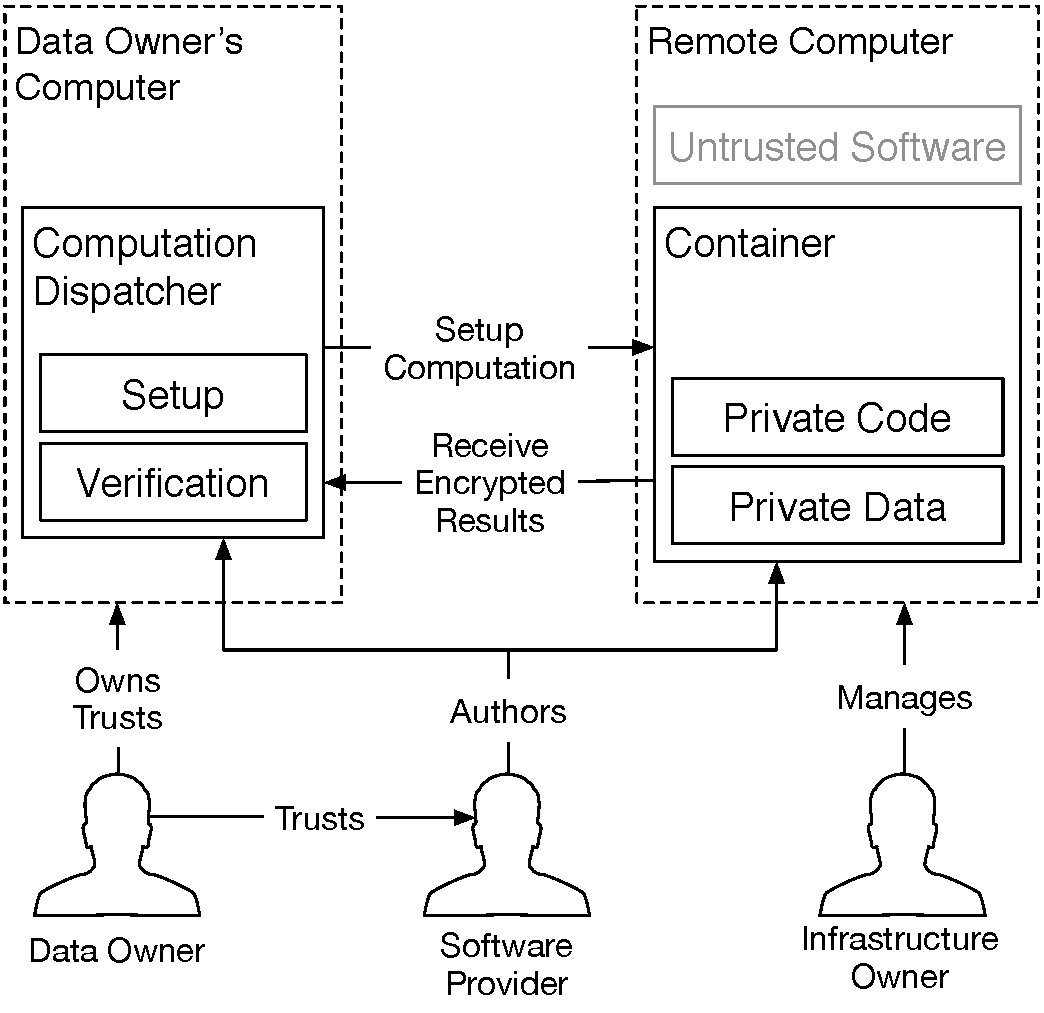
\includegraphics[width=75mm]{figures/remote_computation.pdf}}
  \caption{
    Secure remote computation. A user relies on a remote computer, owned by an
    untrusted party, to perform some computation on her data. The user has some
    assurance of the computation's integrity and privacy.
  }
  \label{fig:remote_computation}
\end{figure}

Intel's Software Guard Extensions (SGX) is the latest iteration in a long line
of trusted computing (Figure~\ref{fig:trusted_computing}) designs, which aim to
solve the secure remote computation problem by leveraging trusted hardware in
the remote computer. The trusted hardware establishes a secure container, and
the remote computation service user uploads the desired computation and data
into the secure container. The trusted hardware protects the data's privacy
and integrity while the computation is being performed on it.

\begin{figure}[hbt]
  \center{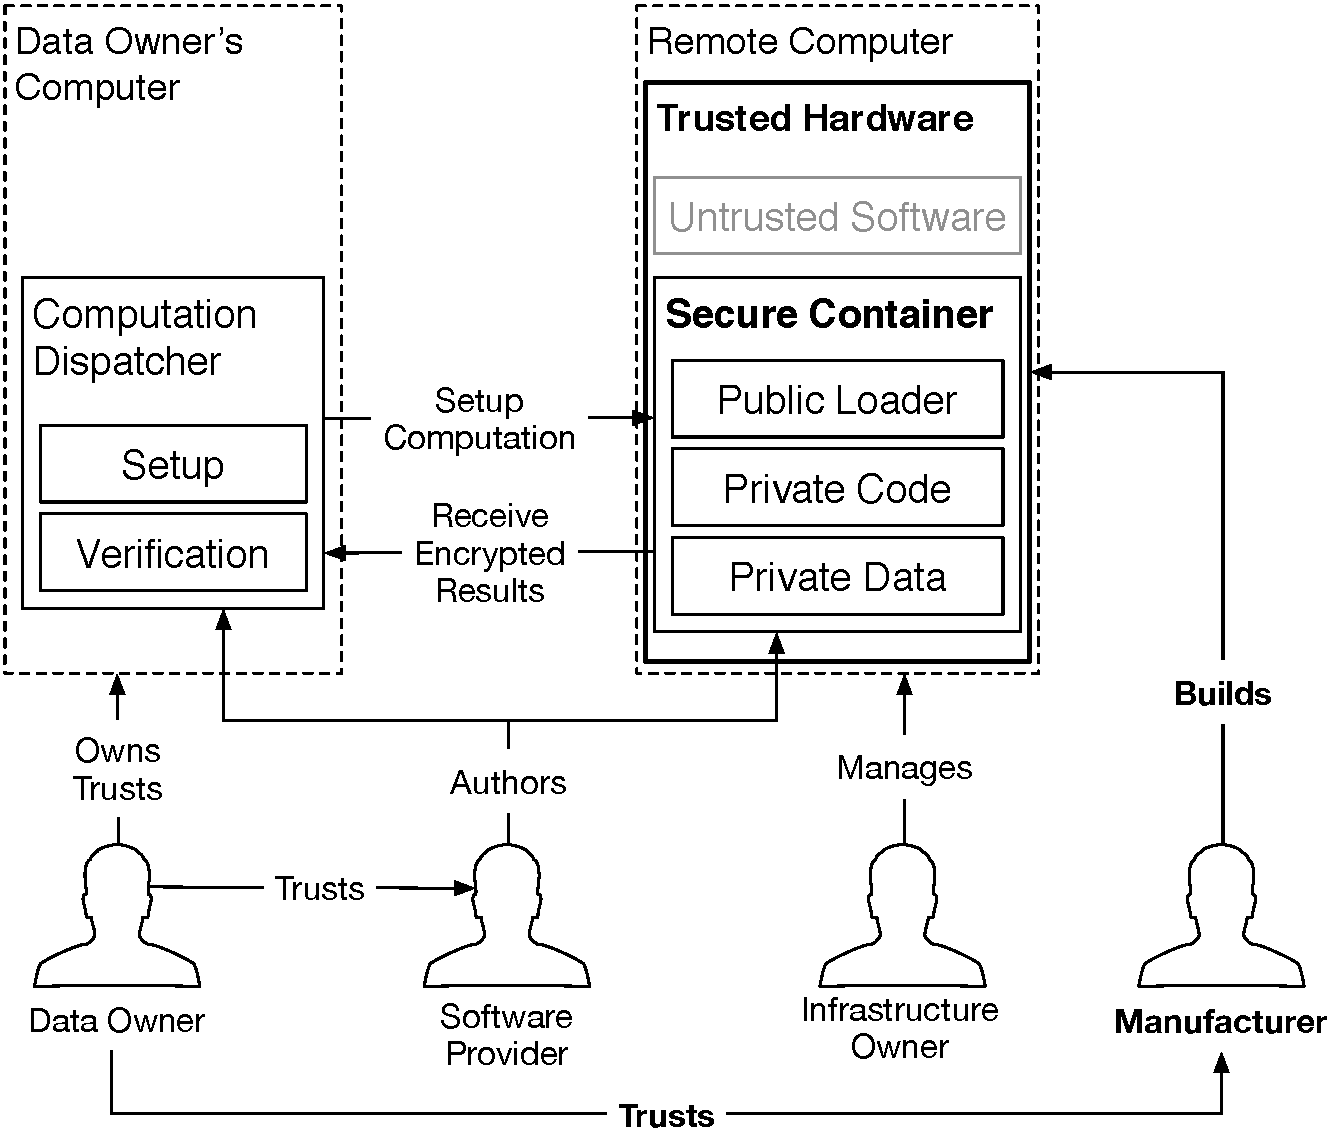
\includegraphics[width=85mm]{figures/trusted_computing.pdf}}
  \caption{
    Trusted computing. The user trusts the manufacturer of a piece of hardware
    in the remote computer, and entrusts her data to a secure container hosted
    by the secure hardware.
  }
  \label{fig:trusted_computing}
\end{figure}

SGX relies on \textit{software attestation}, like its predecessors, the
TPM~\cite{grawrock2003tpm} and TXT~\cite{grawrock2009txt}. Attestation
(Figure~\ref{fig:generic_attestation}) proves to a user that she is
communicating with a specific piece of software running in a secure container
hosted by the trusted hardware. The proof is a cryptographic signature that
certifies the hash of the secure container's contents. It follows that the
remote computer's owner can load any software in a secure container, but the
remote computation service user will refuse to load her data into a secure
container whose contents hash that does not match the expected value.

\begin{figure}[hbt]
  \center{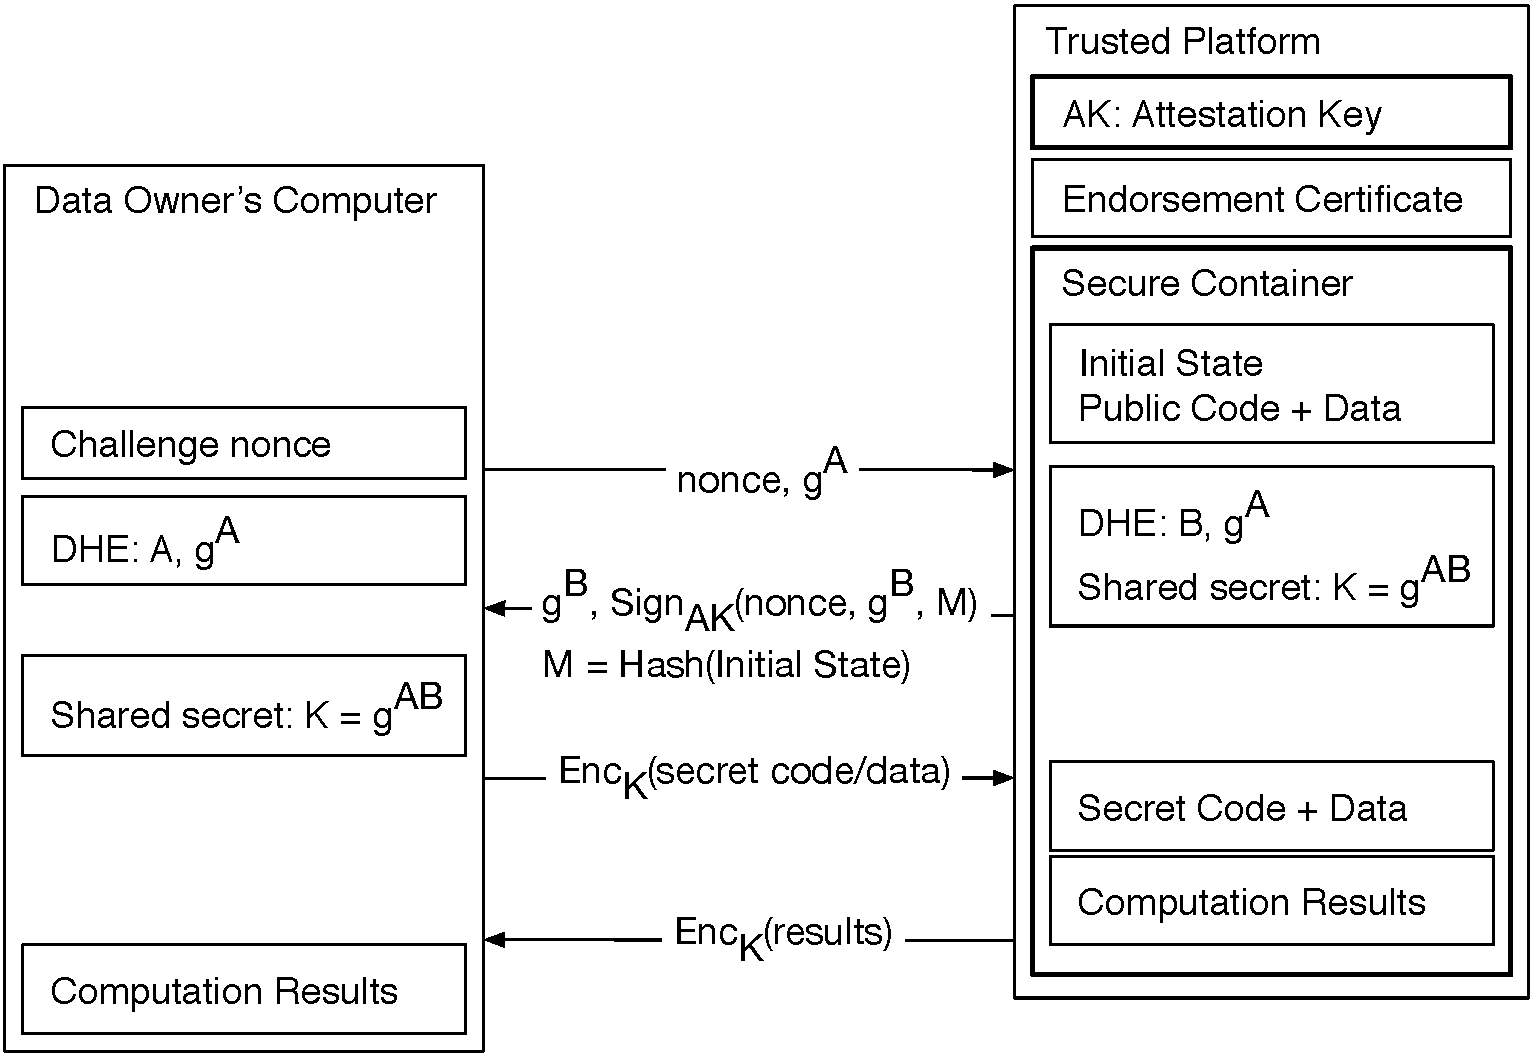
\includegraphics[width=85mm]{figures/generic_attestation.pdf}}
  \caption{
    Software attestation proves to a remote computer that it is communicating
    with a specific secure container hosted by a trusted platform. The proof is
    an attestation signature produced by the platform's secret attestation key.
    The signature covers the container's initial state, a challenge nonce
    produced by the remote computer, and a message produced by the container.
  }
  \label{fig:generic_attestation}
\end{figure}

The remote computation service user verifies the \textit{attestation key} used
to produce the signature against an \textit{endorsement certificate} created by
the trusted hardware's manufacturer. The certificate states that the
attestation key is only known to the trusted hardware, and only used for the
purpose of attestation.

SGX stands out from its predecessors by the amount of code covered by the
attestation, which is in the Trusted Computing Base (TCB) for the system using
hardware protection. The attestations produced by the original TPM design
covered all the software running on a computer, and TXT attestations covered
the code inside a VMX \cite{uhlig2005vmx} virtual machine. In SGX, an
\textit{enclave} (secure container) only contains the private data in a
computation, and the code that operates on it.

For example, a cloud service that performs image processing on confidential
medical images could be implemented by having users upload encrypted images.
The users would send the encryption keys to software running inside an enclave.
The enclave would contain the code for decrypting images, the image processing
algorithm, and the code for encrypting the results. The code that receives the
uploaded encrypted images and stores them would be left outside the enclave.

An SGX-enabled processor protects the integrity and privacy of the computation
inside an enclave by isolating the enclave's code and data from the outside
environment, including the operating system and hypervisor, and hardware
devices attached to the system bus. At the same time, the SGX model remains
compatible with the traditional software layering in the Intel architecture,
where the OS kernel and hypervisor manage the computer's resources.


\subsection{SGX Lightning Tour}
\label{sec:intro_sgx}

SGX sets aside a memory region, called the \textit{Processor Reserved Memory}
(PRM, \S~\ref{sec:prm}). The CPU protects the PRM from all non-enclave memory
accesses, including kernel, hypervisor and SMM (\S~\ref{sec:rings}) accesses,
and DMA accesses (\S~\ref{sec:motherboard}) from peripherals.

The PRM holds the \textit{Enclave Page Cache} (EPC, \S~\ref{sec:epc}), which
consists of 4KB pages that store enclave code and data. The system software,
which is untrusted, is in charge of assigning EPC pages to enclaves. The CPU
tracks each EPC page's state in the \textit{Enclave Page Cache Metadata} (EPCM,
\S~\ref{sec:epcm}), to ensure that each EPC page belongs to exactly one
enclave.

The initial code and data in an enclave is loaded by untrusted system software.
During the setup stage (\S~\ref{sec:lifecycle}), the system software asks the
CPU to copy data from unprotected memory (outside PRM) into EPC pages, and
assigns the pages to the enclave being setup (\S~\ref{sec:epcm}). This
means that the initial enclave state is known to the system software.

After all the enclave's pages are loaded into EPC, the system software asks the
CPU to mark the enclave as initialized, at which point application software can
run the code inside the enclave. After an enclave is initialized, the loading
method described above is disabled.

While an enclave is loaded, its contents is cryptographically hashed by the
CPU. When the enclave is initialized, the hash is finalized, and becomes the
enclave's \textit{measurement hash}.

A remote party can undergo an \textit{attestation} process to convince itself
that it is communicating with a specific enclave running in a secure
environment. The remote party generates a random challenge and sends it to the
enclave. After an intricate sequence of steps, the remote party receives an
\textit{attestation signature} that covers the challenge, the enclave's
measurement hash, and a message generated by the enclave. The attestation
signature is created by a secret CPU attestation key, which is covered by an
\textit{attestation certificate} rooted at Intel's manufacturer key.

Provided that the remote party trusts Intel's root key, attestation convinces
it that the message in the attestation was generated by a specific enclave
running in an SGX environment. If the message is a step in a Diffie-Hellman key
exchange, the remote party can be assured that the resulting symmetric key is
only shared between it and the attested enclave.

\section{Computer Architecture Background}
\label{sec:architecture_background}

This section attempts to summarize the general architectural principles behind
Intel's most popular computer processors, as well as the peculiarities needed
to reason about the security properties of a system running on these
processors. Unless specified otherwise, the information here is summarized from
Intel's \textit{Software Development Manual}~(SDM)~\cite{intel2015sdm}.

Analyzing the security of a software system requires understanding the
interactions between all the parts of the software's execution environment, so
this section is quite long. We do refrain from introducing any security
concepts here, so readers familiar with x86's intricacies can safely skip this
section and refer back to it when necessary.

We use the terms \textit{Intel processor} or \textit{Intel CPU} to refer to the
server and desktop versions of Intel's Core line-up. In the interest of space
and mental sanity, we ignore Intel's other processors, such as the embedded
line of Atom CPUs, or the failed Itanium line. Consequently, the terms
\textit{Intel computers} and \textit{Intel systems} refers to computer systems
built around Intel's Core processors.

In this paper, the term \textit{Intel architecture} refers to the x86
architecture described in Intel's SDM. The x86 architecture is overly complex,
mostly due to the need to support executing legacy software dating back to 1990
directly on the CPU, without the overhead of software interpretation. We only
cover the parts of the architecture visible to modern 64-bit software, also
in the interest of space and mental sanity.

The 64-bit version of the x86 archicture, covered in this section, was actually
invented by Advanced Micro Devices (AMD), and is also known as AMD64,
\texttt{x86\_64}, and x64. The term ``Intel architecture'' highlights our
interest in the architecture's implementation in Intel's chips, and our desire
to understand the mindsets of Intel SGX's designers.


\subsection{Overview}
\label{sec:background_overview}

A computer's main resources~(\S~\ref{sec:resources}) are \textit{memory} and
\textit{processors}. On Intel computers, \textit{Dynamic Random-Access
Memory}~(DRAM) chips~(\S~\ref{sec:motherboard}) provide the memory, and one or
more CPU chips expose \textit{logical processors}~(\S~\ref{sec:cpu_core}).
These resources are managed by \textit{system software}. An Intel computer
typically runs two kinds of system software, namely operating systems and
hypervisors.

The Intel architecture was designed to support runsning multiple application
software instances, called \textit{processes}. An
\textit{operating system}~(\S~\ref{sec:rings}), allocates the computer's
resources to the running processes. Server computers, especially in cloud
environments, may run multiple operating system instances at the same time.
This is accomplished by having a \textit{hypervisor}~(\S~\ref{sec:rings})
partition the computer's resources between the operating system instances
running on the computer.

System software uses virtualization techniques to isolate each piece of
software that it manages (process or operating system) from the rest of the
software running on the computer. This isolation is a key tool for keeping
software complexity at manageable levels, as it allows application and OS
developers to focus on their software, and ignore the interactions with other
software that may run on the computer.

A key component of virtualization is address translation (\S~\ref{sec:paging}),
which is used to give software the impression that it owns all the memory on
the computer. Address translation provides isolation that prevents a piece of
buggy or malicious software from directly damaging other software, by modifying
its memory contents.

The other key component of virtualization is the software privilege levels
(\S~\ref{sec:rings}) enforced by the CPU. Hardware privilege separation ensures
that a piece of buggy or malicious software cannot damage other software
indirectly, by interfering with the system software managing it.

Processes express their computing power requirements by creating execution
\textit{threads}, which are assigned by the operating system to the computer's
logical processors. A thread contains an execution
context~(\S~\ref{sec:registers}), which is the information necessary to
perform a computation. For example, an execution context stores the address of
the next instruction that will be executed by the processor.

Operating systems give each process the illusion that it has an infinite amount
of logical processors at its disposal, and multiplex the available logical
processors between the threads created by each process. Modern operating
systems implement \textit{preemptive multithreading}, where the logical
processors are rotated between all the threads on a system every few
milliseconds. Changing the thread assigned to a logical processor is
accomplished by an execution context switch (\S~\ref{sec:registers}).

Hypervisors expose a fixed number of virtual processors (vCPUs) to each
operating system, and also use context switching to multiplex the logical CPUs
on a computer between the vCPUs presented to the guest operating systems.

The execution core in a logical processor can execute instructions and consume
data at a much faster rate than DRAM can supply them. Many of the complexities
in modern computer architectures stem from the need to cover this speed gap.
Recent Intel CPUs rely on hyper-threading~(\S~\ref{sec:cpu_core}),
out-of-order execution~(\S~\ref{sec:out_of_order}), and
caching~(\S~\ref{sec:caching}), all of which have security implications.

An Intel processor contains many levels of intermediate memories that are much
faster than DRAM, but also orders of magnitude smaller.  The fastest
intermediate memory is the logical processor's register
file~(\S~\ref{sec:resources}, \S~\ref{sec:address_spaces},
\S~\ref{sec:registers}). The other intermediate memories are called
caches~(\S~\ref{sec:caching}). The Intel architecture requires application
software to explicitly manage the register file, which serves as a high-speed
scratch space. At the same time, caches transparently accelerate DRAM requests,
and are mostly invisible to software.

Intel computers have multiple logical processors. As a consequence, they also
have multiple caches distributed across the CPU chip. On multi-socket systems,
the caches are distributed across multiple CPU chips. Therefore, Intel systems
use a cache coherence mechanism~(\S~\ref{sec:cache_coherence}), ensuring that
all the caches have the same view of DRAM. Thanks to cache coherence,
programmers can build software that is unaware of caching, and still runs
correctly in the presence of distributed caches. However, cache coherence does
not cover the dedicated caches used by address translation~(\S~\ref{sec:tlbs}),
and system software must take special measures to keep these caches consistent.

CPUs communicate with the outside world via I/O devices (also known as
peripherals), such as network interface cards and display
adapters~(\S~\ref{sec:computer_map}). Conceptually, the CPU communicates with
the DRAM chips and the I/O devices via a \textit{system bus} that connects all
these components.

Software written for the Intel architecture communicates with I/O devices via
the I/O address space~(\S~\ref{sec:address_spaces}) and via the memory address
space, which is primarily used to access DRAM. System software must configure
the CPU's caches~(\S~\ref{sec:memory_io}) to recognize the memory address
ranges used by I/O devices. Devices can notify the CPU of the occurrence of
events by dispatching interrupts~(\S~\ref{sec:interrupts}), which cause a
logical processor to stop executing its current thread, and invoke a special
handler in the system software~(\S~\ref{sec:faults}).

Intel systems have a highly complex computer initialization
sequence~(\S~\ref{sec:booting}), due to the need to support a large variety of
peripherals, as well as a multitude of operating systems targeting different
versions of the architecture. The initialization sequence is a challenge to any
attempt to secure an Intel computer, and has facilitated many security
compromises~(\S~\ref{sec:rings}).

Intel's engineers use the processor's microcode
facility~(\S~\ref{sec:microcode}) to implement the more complicated aspects of
the Intel architecture, which greatly helps manage the hardware's complexity.
The microcode is completely invisible to software developers, and its design is
mostly undocumented. However, in order to evaluate the feasibility of any
architectural change proposals, one must be able to distinguish changes that
can be implemented in microcode from changes that can only be accomplished by
modifying the hardware.

\subsection{Computational Model}
\label{sec:resources}

This section pieces together a highly simplified model for a computer that
implements the Intel architecture, illustrated in
Figure~\ref{fig:computer_model}. The simplified model is intended to help the
reader's intuition process the fundamental concepts used by the rest of the
paper. The following sections gradually replace the simplified model with a
more accurate description of the Intel architecture.

\begin{figure}[hbt]
  \centering
  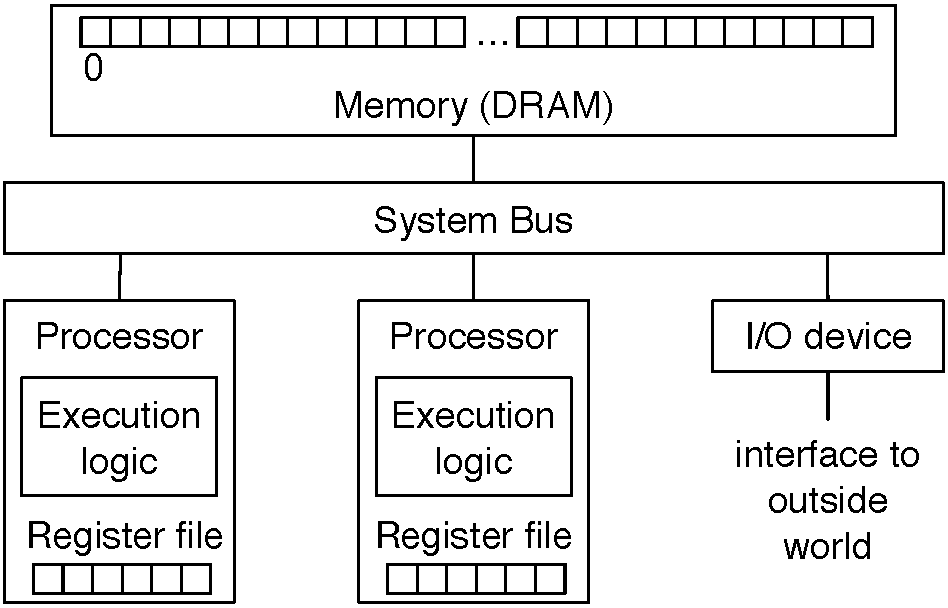
\includegraphics[width=65mm]{figures/computer_model.pdf}
  \caption{
    A computer's core is its processors and memory, which are connected by a
    system bus. Computers also have I/O devices, such as keyboards, which are
    also connected to the processor via the system bus.
  }
  \label{fig:computer_model}
\end{figure}


The building blocks for the model presented here come from
\cite{saltzer2009systemdesign}, which introduces the key abstractions in a
computer system, and  then focuses on the techniques used to build software
systems on top of these abstractions.

The memory is an array of storage cells, addressed using natural numbers
starting from 0, and implements the abstraction depicted in
Figure~\ref{fig:memory_abstraction}. Its salient feature is that the result of
reading a memory cell at an address must equal the most value written to that
memory cell.

\begin{figure}[hbt]
  \centering
  \begin{tabularx}{\columnwidth}{| X |}
  \hline
  \textsc{write}(\textit{addr}, \textit{value}) $ \rightarrow \varnothing $ \\
  Store \textit{value} in the storage cell identified by \textit{addr}. \\
  \hline
  \textsc{read}(\textit{addr}) $ \rightarrow $ \textit{value} \\
  Return the \textit{value} argument to the most recent \textsc{write} call
  referencing \textit{addr}. \\
  \hline
  \end{tabularx}
  \caption{The memory abstraction}
  \label{fig:memory_abstraction}
\end{figure}

A logical processor repeatedly reads \textit{instructions} from the
computer's memory and executes them, according to the flowchart in
Figure~\ref{fig:processor_execution}.

\begin{figure}[hbt]
  \centering
  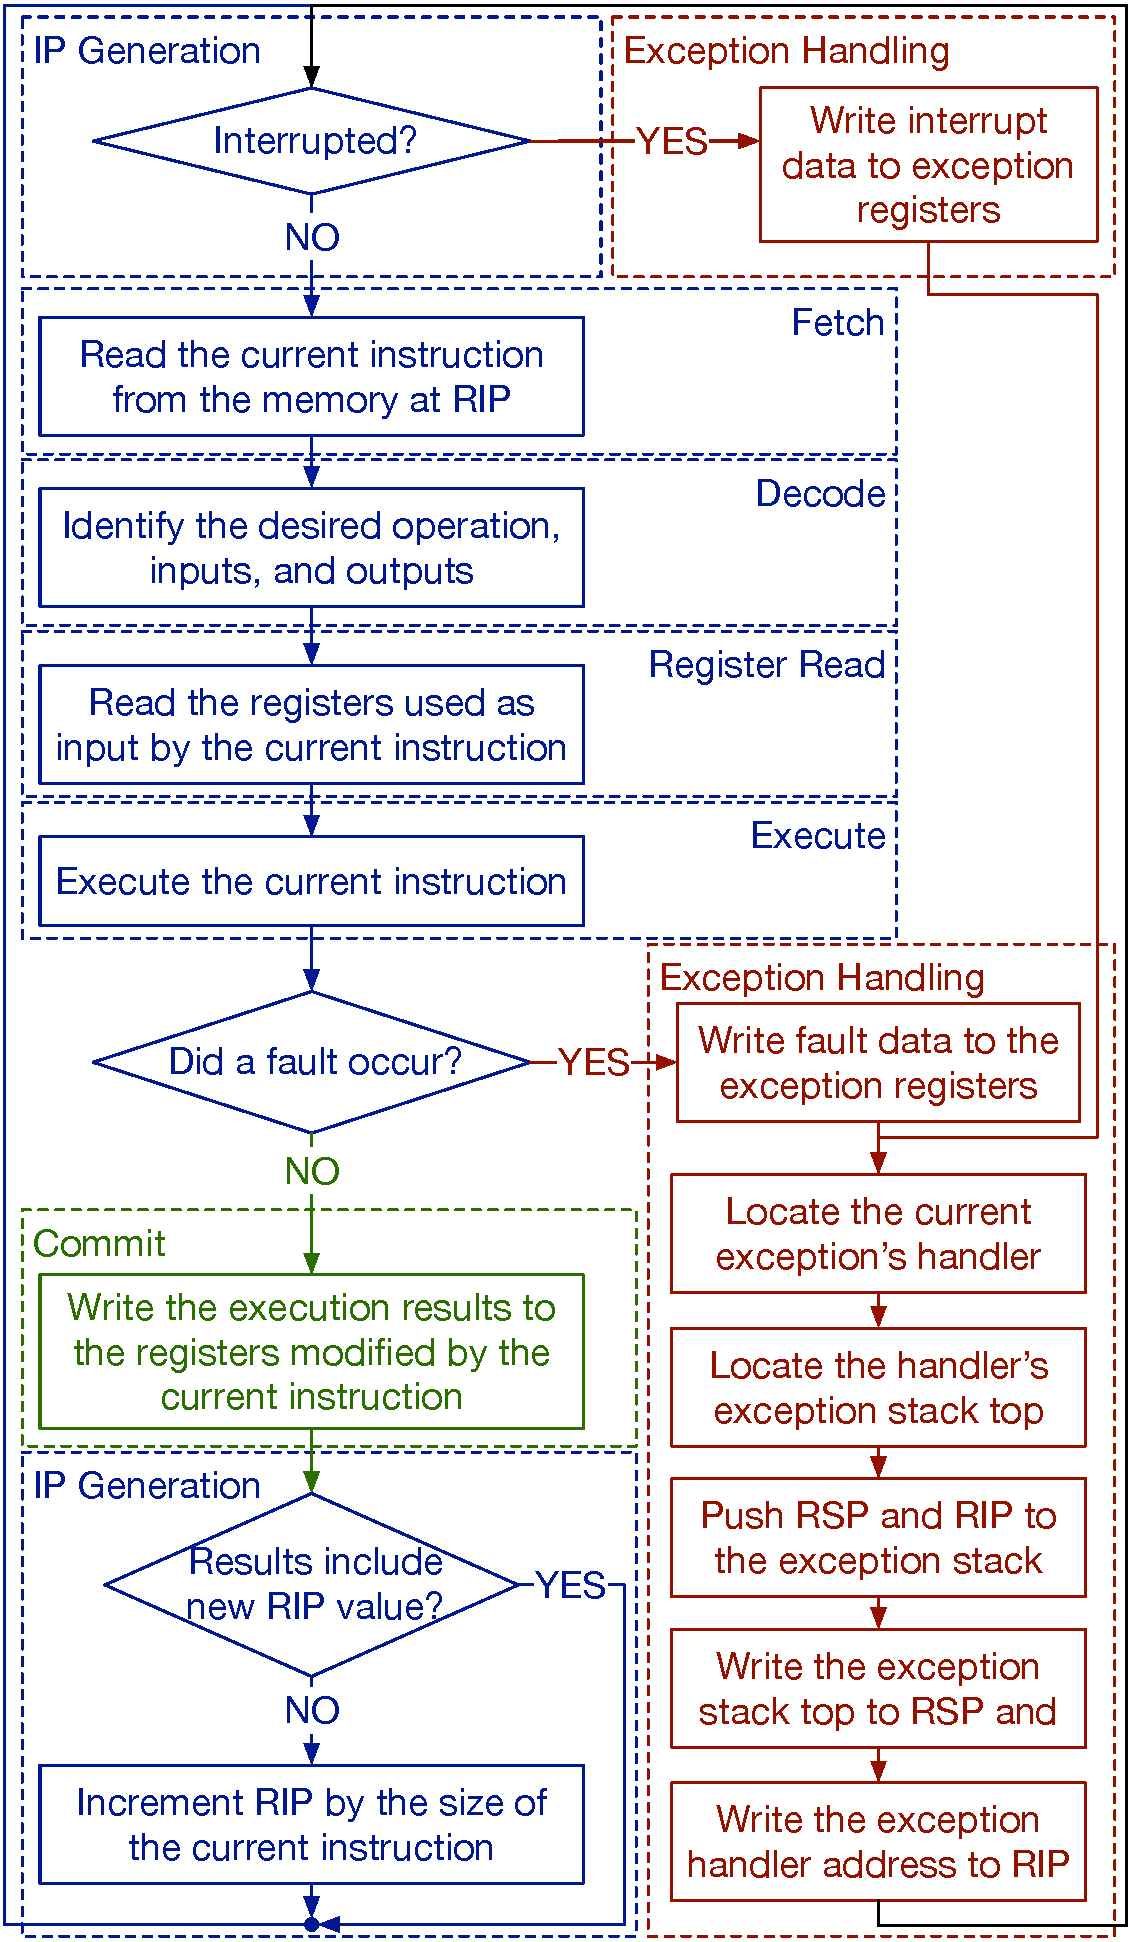
\includegraphics[width=85mm]{figures/processor_execution.pdf}
  \caption{
    A processor fetches instructions from the memory and executes them. The RIP
    register holds the address of the instruction to be executed.
  }
  \label{fig:processor_execution}
\end{figure}

The processor has an internal memory, referred to as the
\textit{register file}. The register file's memory cells, generally known as
\textit{registers}, make up the \textit{execution context} used to execute
instructions.

An instruction performs a simple computation on its inputs and stores the
result in an output location. For example, \texttt{ADD RDX, RAX, RBX} performs
an integer addition, where the inputs are the registers RAX and RBX, and the
result is stored in the output register RDX.

The registers mentioned in Figure~\ref{fig:processor_execution} are the
\textit{instruction pointer}~(RIP), which stores the memory  address of the
next instruction to be executed by the processor, and the
\textit{stack pointer}~(RSP), which stores the memory address of the topmost
element in the call stack used by the processor's procedural programming
support. The other execution context registers are described in
\S~\ref{sec:address_spaces} and \S~\ref{sec:registers}.

Under normal circumstances, the processor repeatedly reads an instruction from
the memory address stored in RIP, executes the instruction, and updates RIP to
point to the following instruction. Unlike many RISC architectures, the Intel
architecture uses a variable-size instruction encoding, so the size of an
instruction is not known until the instruction has been read from memory.

While executing an instruction, the processor may encounter a \textit{fault},
which is a situation where the instruction's preconditions are not met. When
a fault occurs, the instruction does not store a result in the output location.
Instead, the instruction's result is considered to be the fault that occurred.
For example, an integer division instruction \texttt{DIV} where the divisor is
zero results in a Division Fault (\#DIV).

When an instruction results in a fault, the processor stops its normal
execution flow, and performs the fault handler process documented in
\S~\ref{sec:faults}. In a nutshell, the processor first looks up the address of
the code that will handle the fault, based on the fault's nature, and sets up
the execution environment in preparation to execute the fault handler.

The processors are connected to each other and to the memory via a
\textit{system bus}, which is a broadcast network that implements the
abstraction in Figure~\ref{fig:bus_abstraction}.

\begin{figure}[hbt]
  \centering
  \begin{tabularx}{\columnwidth}{| X |}
  \hline
  \textsc{send}(\textit{op}, \textit{addr}, \textit{data})
  $ \rightarrow \varnothing $ \\
  Place a message containing the operation code \textit{op}, the bus address
  \textit{addr}, and the value \textit{data} on the bus. \\
  \hline
  \textsc{read}() $ \rightarrow $ (\textit{op}, \textit{addr},
  \textit{value}) \\
  Return the message that was written on the bus at the beginning of this
  clock cycle. \\
  \hline
  \end{tabularx}
  \caption{The system bus abstraction}
  \label{fig:bus_abstraction}
\end{figure}

During each clock cycle, at most one of the devices connected to the system bus
can send a message, which is received by all the other devices connected to the
bus. Each device attached to the bus decodes the operation codes and addresses
of all the messages sent on the bus and ignores the messages that do not
require its involvement.

For example, when the processor wishes to read a memory location, it sends a
message with the operation code \textsc{read-request} and the bus address
corresponding to the desired memory location. The memory sees the message on
the bus and performs the \textsc{read} operation. At a later time, the memory
responds by sending a message with the operation code \textsc{read-response},
the same address as the request, and the data value set to the result of the
\textsc{read} operation.

The computer communicates with the outside world via I/O devices, such as
keyboards, displays, and network cards, which are connected to the system bus.
Devices mostly respond to requests issued by the processor. However, devices
also have the ability to issue \textit{interrupt requests} that notify the
processor of outside events, such as the user pressing a key on a keyboard.

Interrupt triggering is discussed in \S~\ref{sec:interrupts}. On modern
systems, devices send interrupt requests by issuing writes to special bus
addresses. Interrupts are considered to be \textit{hardware exceptions}, just
like faults, and are handled in a similar manner.

\subsection{Software Privilege Levels}
\label{sec:rings}

In an Infrastructure-as-a-Service (IaaS) cloud environment, such as Amazon EC2,
commodity CPUs run software at four different privilege levels. The rest of the
section describes the privilege levels. We also point to successful exploits
that execute at each privilege level, motivating the SGX design decision to
assume that the host computer has malicious software running at all privilege
levels.

Figure~\ref{fig:cpu_rings} shows the privilege levels in the Intel
architecture. Software running at each level is strictly more powerful than
software running at less privileged levels. It follows that software running at
a level can access the code and data at less privileged levels, and compromise
the software running at these levels. Thus, software at each level must trust
all the software running at more privileged levels.

\begin{figure}[hbtp]
  \centering
  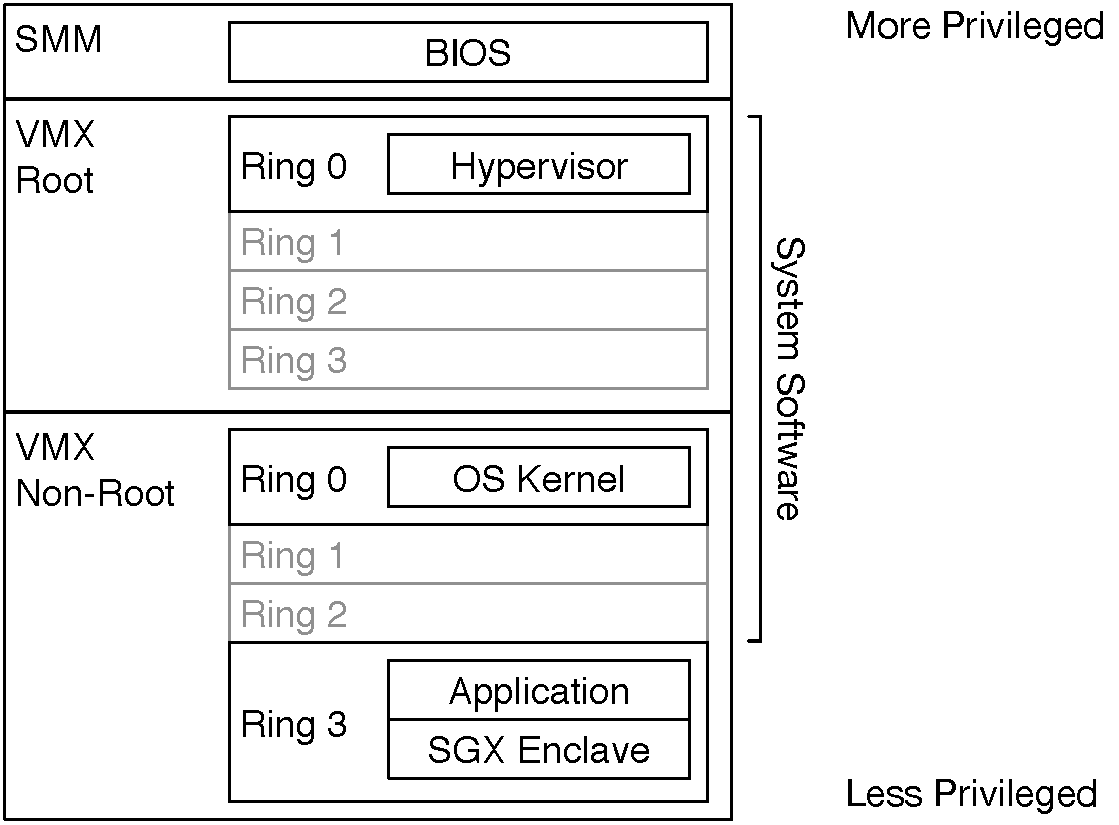
\includegraphics[width=85mm]{figures/cpu_rings.pdf}
  \caption{
    The privilege levels in the x86 architecture, and the software that
    typically runs at each security level.
  }
  \label{fig:cpu_rings}
\end{figure}

% System Management Mode: SDM S 34

\textit{System Management Mode} (SMM) is intended for use by the motherboard
manufacturers to implement features such as fan control and deep sleep, and/or
to emulate missing hardware. SMM mode is entered by sending the CPU an SMI
signal, which was initially designed exclusively for hardware use, and only
produced when the SMI\# pin was asserted on the CPU's chip package. However, in
modern systems, system software can generate an SMI, using the methods in
\S~\ref{sec:interrupts}. This opens up the avenue for SMM-based software
exploits.

The SMM code and data are stored in a contiguous subset of DRAM called
\textit{System Management RAM} (SMRAM) which, in theory, is not readable or
writable when the processor isn't running in SMM. However, its protection
mechanisms were bypassed multiple times~\cite{duflot2006smm,
rutkowska2008remap, wojtczuk2009smm, kallenberg2014smm}, and SMM-based
rootkits~\cite{wecherowski2009smm, embleton2010smm} have been demonstrated.

IaaS cloud providers allow their customers to run their operating system of
choice in a virtualized environment. Hardware
virtualization~\cite{uhlig2005vmx}, called \textit{Virtual Machine Extensions}
(VMX) by Intel, adds support for a \textit{hypervisor}, also called a
Virtual Machine Monitor (VMM) in the Intel documentation. The hypervisor runs
at a higher privilege level (VMX root mode) than the operating system, and is
responsible for allocating hardware resources across multiple operating systems
that share the same physical machine. The hypervisor uses the CPU's hardware
virtualization features to make each operating system believe it is running in
its own computer, called a \textit{virtual machine} (VM). Hypervisor code
generally runs at ring 0 in VMX root mode.

The popular Xen hypervisor uses VMX root mode to obtain better peformance and a
smaller codebase \cite{zhang2008xen} than virtualization software based on
binary translation \cite{rosenblum2005virtualization}. Despite its relatively
small codebase, Xen has had over 40 security vulnerabilities patched in
\textbf{each} of the last three years (2012-2014) \cite{cvedetails2014xen}.

\cite{mccune2010trustvisor} proposes using a very small hypervisor together
with Intel TXT's dynamic root of trust for measurement (DRTM) to implement
trusted execution. \cite{vasudevan2010requirements} argues that a dynamic root
of trust mechanism, like Intel TXT, is necessary to ensure a hypervisor's
integrity.  Unfortunately, the TXT design requires an implementation complex
enough that security vulnerabilities have been found \cite{wojtczuk2009txt2}
\cite{wojtczuk2011txt}. Furthermore, any SMM attack can be used to compromise
TXT \cite{wojtczuk2009txt}.

The systems research literature recommends breaking up an operating system into
a small \textit{kernel}, which runs at a high privilege level, known as the
\textit{kernel mode} or \textit{supervisor mode} and, in the Intel
architecture, as \textit{ring 0}. The kernel allocates the computer's resources
to the other system components, such as device drivers and services, which run
at lower privilege levels. However, for performance reasons\footnote{Switching
between rings is much slower than a normal procedure call.}, mainstream
operating systems have large amounts of code running at ring 0. Their
\textit{monolithic kernels} include device drivers, filesystem code, networking
stacks, and video rendering functionality.

The monolithic kernel design leads to many opportunities for security
vulnerabilities in kernel code. For example the Linux kernel has had over 100
security vulnerabilities patched in \textbf{each} of the last three years
(2012-2014) \cite{cvedetails2014linux} \cite{chen2011linux}. Also, a successful
attack on SMM or the hypervisor trivially translates into a compromised kernel.

Application code, such as a Web server or a game client, runs at the lowest
privilege level, referred to as \textit{user mode} (\textit{ring 3} in the
Intel architecture). In IaaS cloud environments, the virtual machine images
provided by customers run in VMX non-root mode, so the kernel runs in VMX
non-root ring 0, and the application code runs in VMX non-root ring 3.

\subsection{Address Spaces}
\label{sec:address_spaces}

While performing computation, a commodity Intel CPU moves data between four
distinct physical address spaces, shown in Figure~\ref{fig:address_spaces}. The
address spaces overlap partially, in both purpose and contents, which can lead
to confusion. This section gives a high-level overview of the physical address
spaces defined by the Intel architecture, with an emphasis on their purpose and
the methods used to manage them.

\begin{figure}[hbtp]
  \center{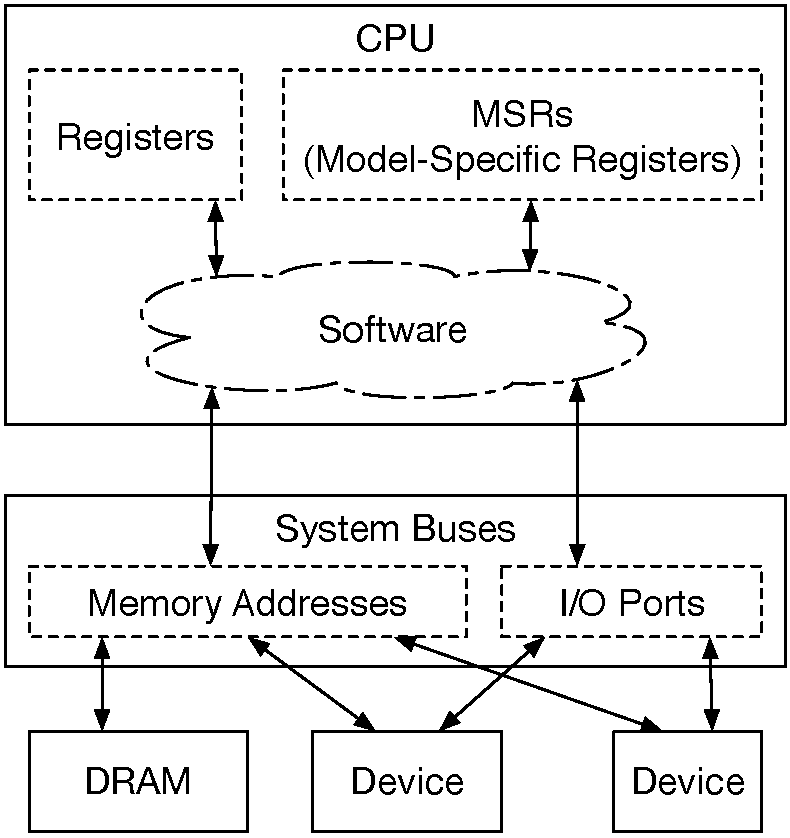
\includegraphics[width=55mm]{figures/address_spaces.pdf}}
  \caption{
    The four physical address spaces used by an Intel CPU. The registers and
    MSRs are internal to the CPU, while the memory and I/O address spaces are
    used to communicate with DRAM and other devices via system buses.
  }
  \label{fig:address_spaces}
\end{figure}

The \textit{register} space consists of names that are used to access the CPU's
register file, which is the only memory that operates at the CPU's clock
frequency and can be used without any latency penalty. The register space is
defined by the CPU's architecture, and documented in the SDM.

Some registers, such as the \textit{Control Registers} (CRs) play specific
roles in configuring the CPU's operation. For example, CR3 plays a central role
in address translation (\S~\ref{sec:paging}). These registers can only be
accessed by system software. The rest of the registers make up an application's
\textit{execution context} (\S~\ref{sec:registers}), which is essentially a
high-speed scratch space. These registers can by accessed at all privilege
levels, and their allocation is managed by the software's compiler. Many CPU
instructions only operate on data in registers, and only place their results in
registers.

The \textit{memory} space, generally referred to as \textit{the address space}
\textit{the physical address space}, consists of $2^{36}$ (64 GB) - $2^{40}$
(1 TB) addresses. The memory space is primarily used to access
\textit{Dynamic Random-Access Memory} (DRAM), the computer's main memory, but
it is also used to communicate with \textit{memory-mapped devices} that read
memory requests off a system bus and write replies for the CPU. Some CPU
instructions can read their inputs from the memory space, or store the results
using the memory space.

A better-known example of memory mapping is that at computer startup, memory
addresses 0xFFFFF000 - 0xFFFFFFFF (the 64 KB of memory right below the 4 GB
mark) are mapped to a flash memory device that holds the code for booting the
computer.

This memory space is partitioned between devices and DRAM by the computer's
firmware during the boot stage. Sometimes, system software includes
motherboard-specific code that modifies the memory space partitioning. The OS
kernel relies on address translation, described in \S~\ref{sec:paging}, to
control the applications' access to the memory space. The hypervisor relies on
the same mechanism to control the guest OSes.

% I/O Address Space: SDM vol1 S 16.3

The \textit{input/output} (I/O) space consists of $2^{16}$ I/O addresses,
usually called \textit{ports}. The I/O ports are used exclusively to
communicate with devices. The CPU provides specific instructions for reading
from and writing to the I/O space. I/O ports are allocated to devices by formal
or de-facto standards. For example, ports 0xCF8 and 0xCFC are always used to
access the PCI express (\S~\ref{sec:motherboard}) configuration space.

The CPU implements a mechanism for system software to provide fine-grained I/O
access to applications. However, all modern kernels restrict application
software from accessing the I/O space directly, in order to limit the damage
potential of application bugs.

% Architectural MSRs: SDM S 35.1
% Time-Stamp Counter: SDM S 17.13

The \textit{Model-Specific Register} (MSR) space consists of $2^{32}$ MSRs,
which are used to configure the CPU's operation. The MSR space was initially
intended for the use of CPU model-specific firmware, but some MSRs have been
promoted to \textit{architectural MSR} status, making their semantics a part of
the Intel architecture. For example, architectural MSR 0x10 holds a
high-resolution monotonically increasing time-stamp counter.

The CPU provides instructions for reading from and writing to the MSR space.
The instructions can only be used by system software. Some MSRs are also
exposed by instructions accessible to applications. For example, applications
can read the time-stamp counter with the \texttt{RDTSC} and \texttt{RDTSCP},
which are very useful for benchmarking and optimizing software, but also for
mounting timing attacks.

\HeadingLevelB{Address Translation}
\label{sec:paging}

% Outcome: understanding the isolation provided by address translation

System software relies on the CPU's address translation mechanism for
implementing isolation among less privileged pieces of software (applications
or operating systems). Virtually all secure architecture designs bring changes
to address translation. We summarize the Intel architecture's address
translation features that are most relevant when establishing a system's
security properties, and refer the reader to \cite{jacob1998virtual} for a more
general presentation of address translation concepts and its other uses.


\HeadingLevelC{Address Translation Concepts}
\label{sec:paging_concepts}
\label{sec:paging_vpn}
\label{sec:paging_ppn}

From a systems perspective, address translation is a layer of indirection
(shown in Figure~\ref{fig:address_translation}) between the
\textit{virtual addresses}, which are used by a program's memory load and store
instructions, and the \textit{physical addresses}, which reference the physical
address space (\S~\ref{sec:address_spaces}). The mapping between virtual and
physical addresses is defined by \textit{page tables}, which are managed by the
system software.

\begin{figure}[hbt]
  \centering
  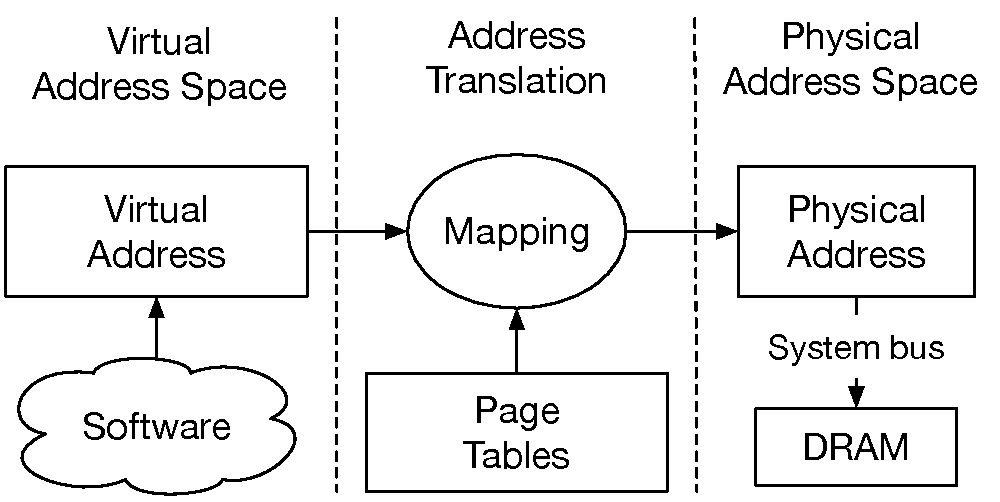
\includegraphics[width=75mm]{figures/address_translation.pdf}
  \caption{
    Virtual addresses used by software are translated into physical memory
    addresses using a mapping defined by the page tables.
  }
  \label{fig:address_translation}
\end{figure}

Operating systems use address translation to implement the \textit{virtual
memory abstraction}, illustrated by Figure~\ref{fig:virtual_memory}. The
virtual memory abstraction exposes the same interface as the memory abstraction
in \S~\ref{sec:resources}, but each process uses a separate virtual address
space that only references the memory allocated to that process. From an
application developer standpoint, virtual memory can be modeled by pretending
that each process runs on a separate computer and has its own DRAM.

\begin{figure}[hbt]
  \centering
  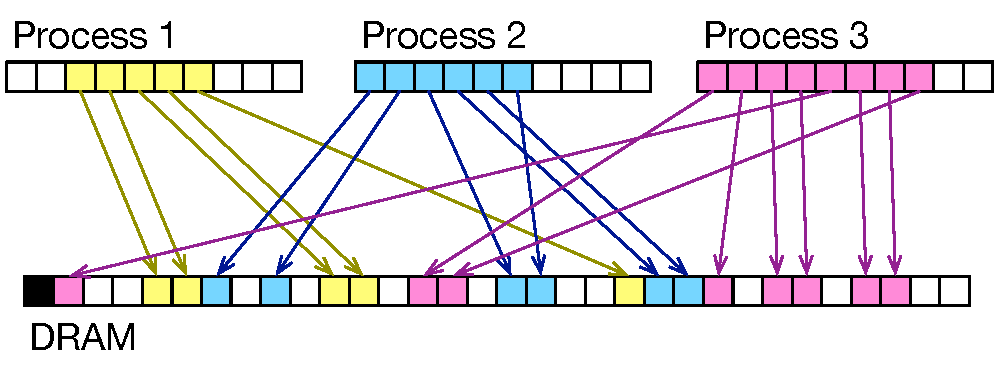
\includegraphics[width=80mm]{figures/virtual_memory.pdf}
  \caption{
    The virtual memory abstraction gives each process its own virtual address
    space. The operating system multiplexes the computer's DRAM between the
    processes, while application developers build software as if it owns the
    entire computer's memory.
  }
  \label{fig:virtual_memory}
\end{figure}

Address translation is used by the operating system to multiplex DRAM among
multiple application processes, isolate the processes from each other, and
prevent application code from accessing memory-mapped devices directly. The
latter two protection measures prevent an application's bugs from impacting
other applications or the OS kernel itself. Hypervisors also use address
translation, to divide the DRAM among operating systems that run concurrently,
and to virtualize memory-mapped devices.

% Canonical Addressing: SDM vol1 S 3.3.7.1
% IA-32e Paging: SDM S 4.5

The address translation mode used by 64-bit operating systems, called
IA-32e by Intel's documentation, maps 48-bit \textit{virtual addresses} to
\textit{physical addresses} of at most 52 bits\footnote{The size of a
physical address is CPU-dependent, and is 40 bits for recent desktop CPUs and
44 bits for recent high-end server CPUs.}. The translation process, illustrated
in Figure~\ref{fig:os_paging}, is carried out by dedicated hardware in the CPU,
which is referred to as the \textit{address translation unit} or the
\textit{memory management unit} (MMU).

\begin{figure}[hbt]
  \centering
  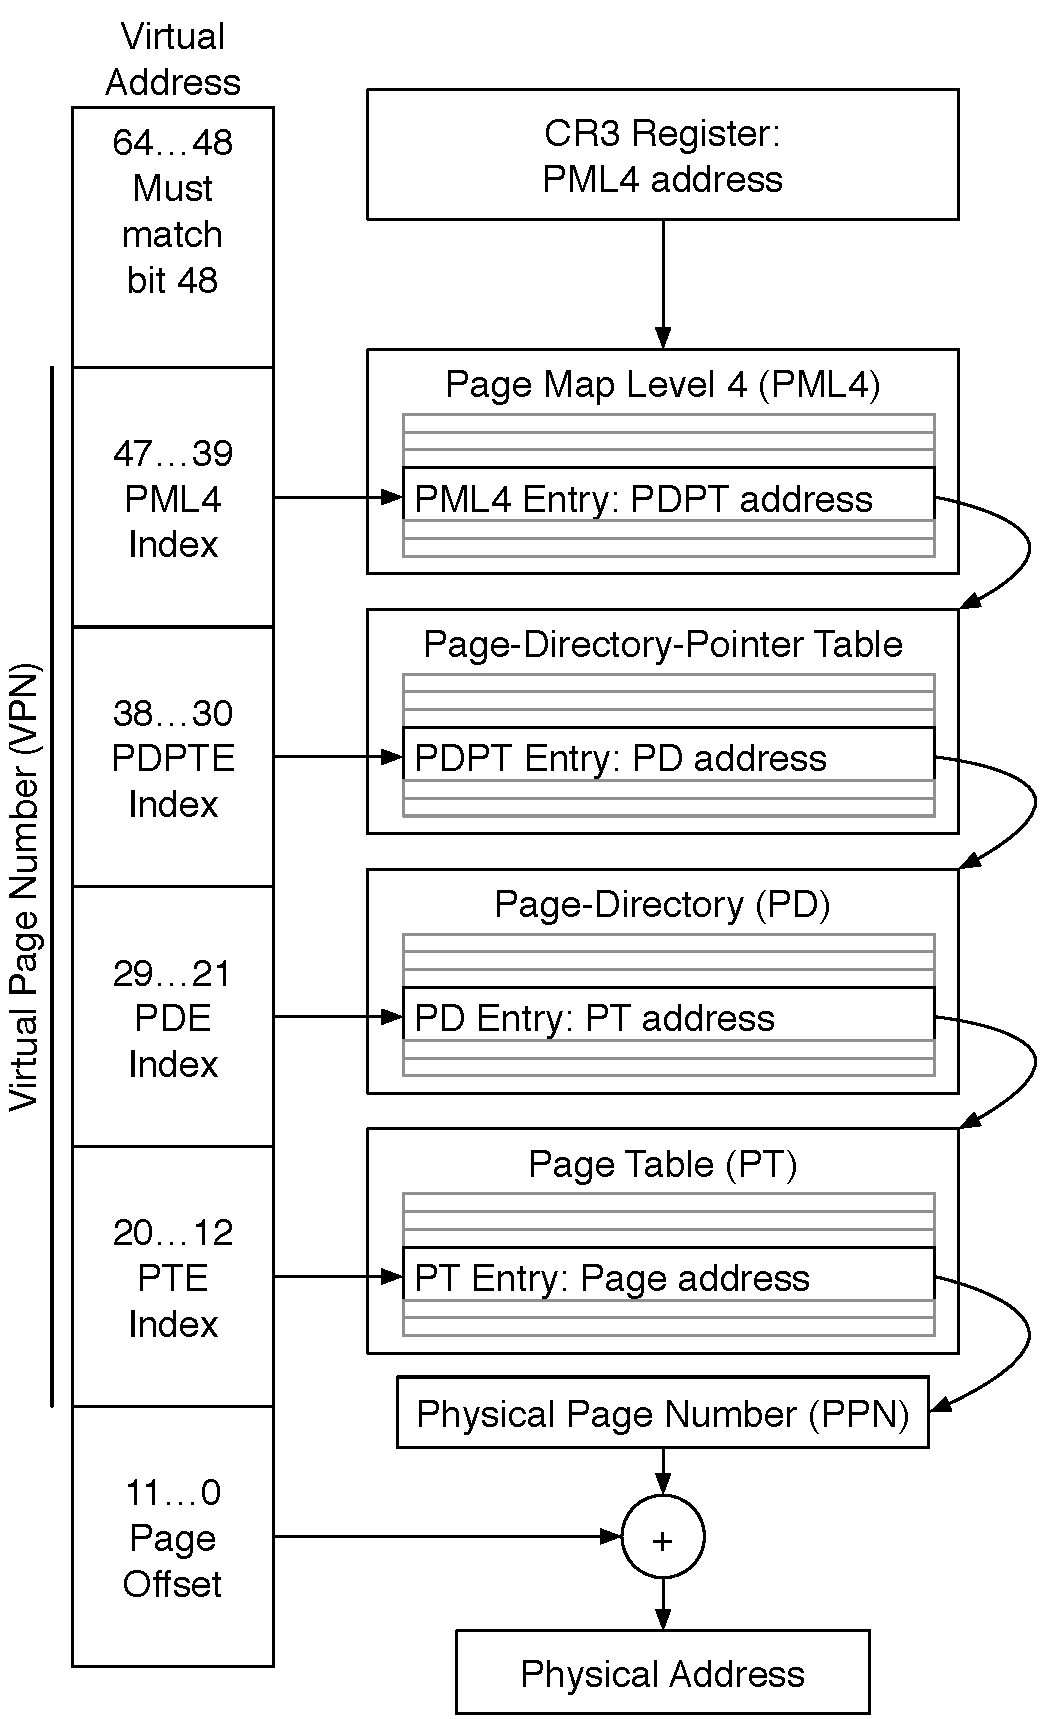
\includegraphics[width=80mm]{figures/os_paging.pdf}
  \caption{
    IA-32e address translation takes in a 48-bit virtual address and outputs
    a 52-bit physical address.
  }
  \label{fig:os_paging}
\end{figure}

The bottom 12 bits of a virtual address are not changed by the translation. The
top 36 bits are grouped into four 9-bit indexes, which are used to index into
the page tables. Despite its name, the page tables data structure closely
resembles a full 512-ary search tree where nodes have fixed keys. Each
node is represented in DRAM as an array of 512 8-byte entries that contain the
physical addresses of the next-level children as well as some flags. The
physical address of the root node is stored in the CR3 register. The arrays in
the last-level nodes contain the physical addresses that are the result of the
address translation.

The address translation function, which does not change the bottom bits of
addresses, partitions the memory address space into \textit{pages}. A page is
the set of all memory locations that only differ in the bottom bits which are
not impacted by address translation, so all the memory addresses in a virtual
page translate to corresponding addresses in the same physical page. From this
perspective, the address translation function can be seen as a mapping between
\textit{Virtual Page Numbers} (VPN) and \textit{Physical Page Numbers} (PPN),
as shown in Figure~\ref{fig:address_translation_bits}.

\begin{figure}[hbt]
  \centering
  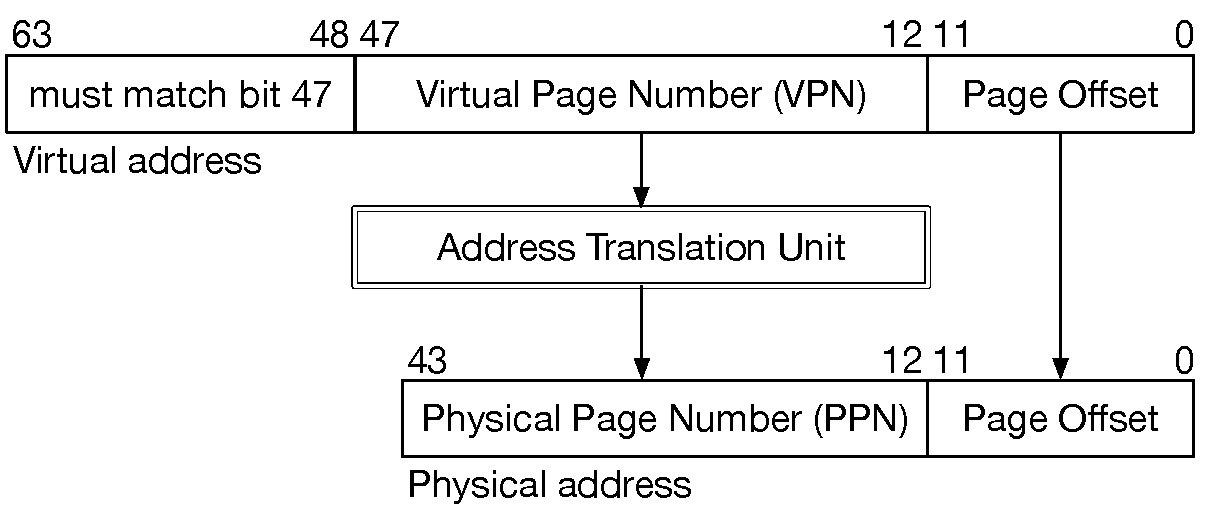
\includegraphics[width=85mm]{figures/address_translation_bits.pdf}
  \caption{
    Address translation can be seen as a mapping between virtual page numbers
    and physical page numbers.
  }
  \label{fig:address_translation_bits}
\end{figure}

In addition to isolating application processes, operating systems also use the
address translation feature to run applications whose collective memory
demands exceed the amount of DRAM installed in the computer. The OS evicts
infrequently used memory pages from DRAM to a larger (but slower) memory, such
as a hard disk drive (HDD) or solid-state drive (SSD). For historical reason,
this slower memory is referred to as the \textit{disk}.

The OS ability to over-commit DRAM is often called \textit{page swapping}, for
the following reason. When an application process attempts to access a page
that has been evicted, the OS ``steps in'' and reads the missing page back into
DRAM. In order to do this, the OS might have to evict a different page from
DRAM, effectively swapping the contents of a DRAM page with a disk page. The
details behind this high-level description are covered in the following
sections.

The CPU's address translation is also referred to as ``paging'', which is a
shorthand for ``page swapping''.


\HeadingLevelC{Address Translation and Virtualization}
\label{sec:vmx_paging}

% VMX Support for Address Translation: SDM S 4.11

Computers that take advantage of hardware virtualization use a hypervisor to
run multiple operating systems at the same time. This creates some tension,
because each operating system was written under the assumption that it owns the
entire computer's DRAM. The tension is solved by a second layer of address
translation, illustrated in Figure~\ref{fig:vmx_address_translation}.

\begin{figure}[hbt]
  \centering
  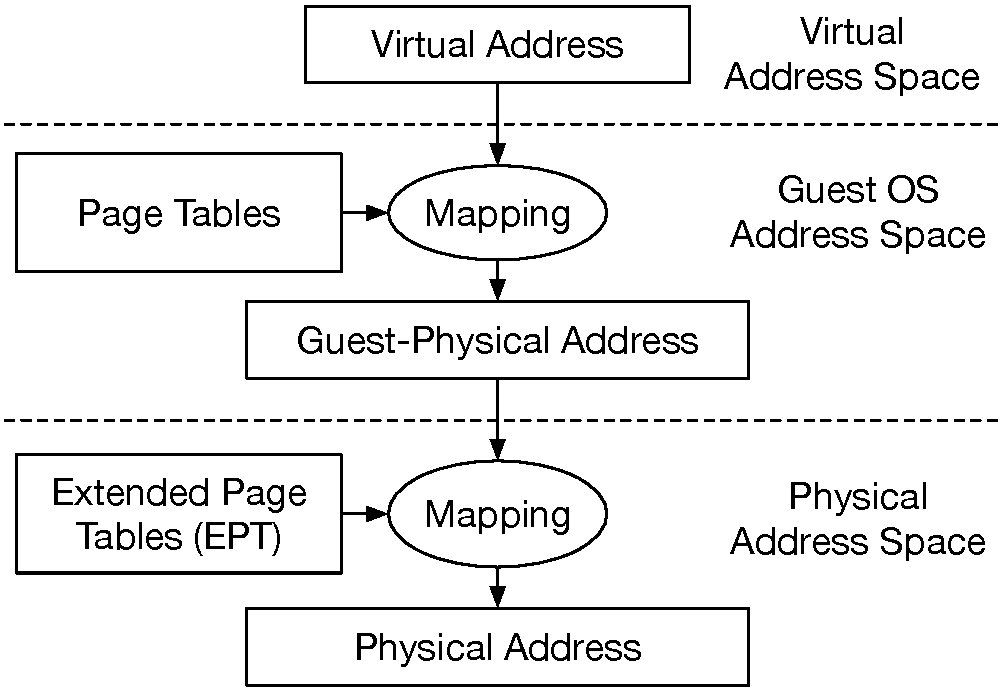
\includegraphics[width=70mm]{figures/vmx_address_translation.pdf}
  \caption{
    Virtual addresses used by software are translated into physical memory
    addresses using a mapping defined by the page tables.
  }
  \label{fig:vmx_address_translation}
\end{figure}


When a hypervisor is active, the page tables set up by an operating system map
between virtual addresses and \textit{guest-physical addresses} in a
\textit{guest-physical address space}. The hypervisor multiplexes the
computer's DRAM between the operating systems' guest-physical address spaces
via the second layer of address translations, which uses \textit{extended page
tables}~(EPT) to map guest-physical addresses to physical addresses.

The EPT uses the same data structure as the page tables, so the process of
translating guest-physical addresses to physical addresses follows the same
steps as IA-32e address translation. The main difference is that the physical
address of the data structure's root node is stored in the extended page table
pointer~(EPTP) field in the \textit{Virtual Machine Control Structure}~(VMCS)
for the guest OS. Figure~\ref{fig:vmx_paging} illustrates the address
translation process in the presence of hardware virtualization.

\begin{figure}[hbt]
  \centering
  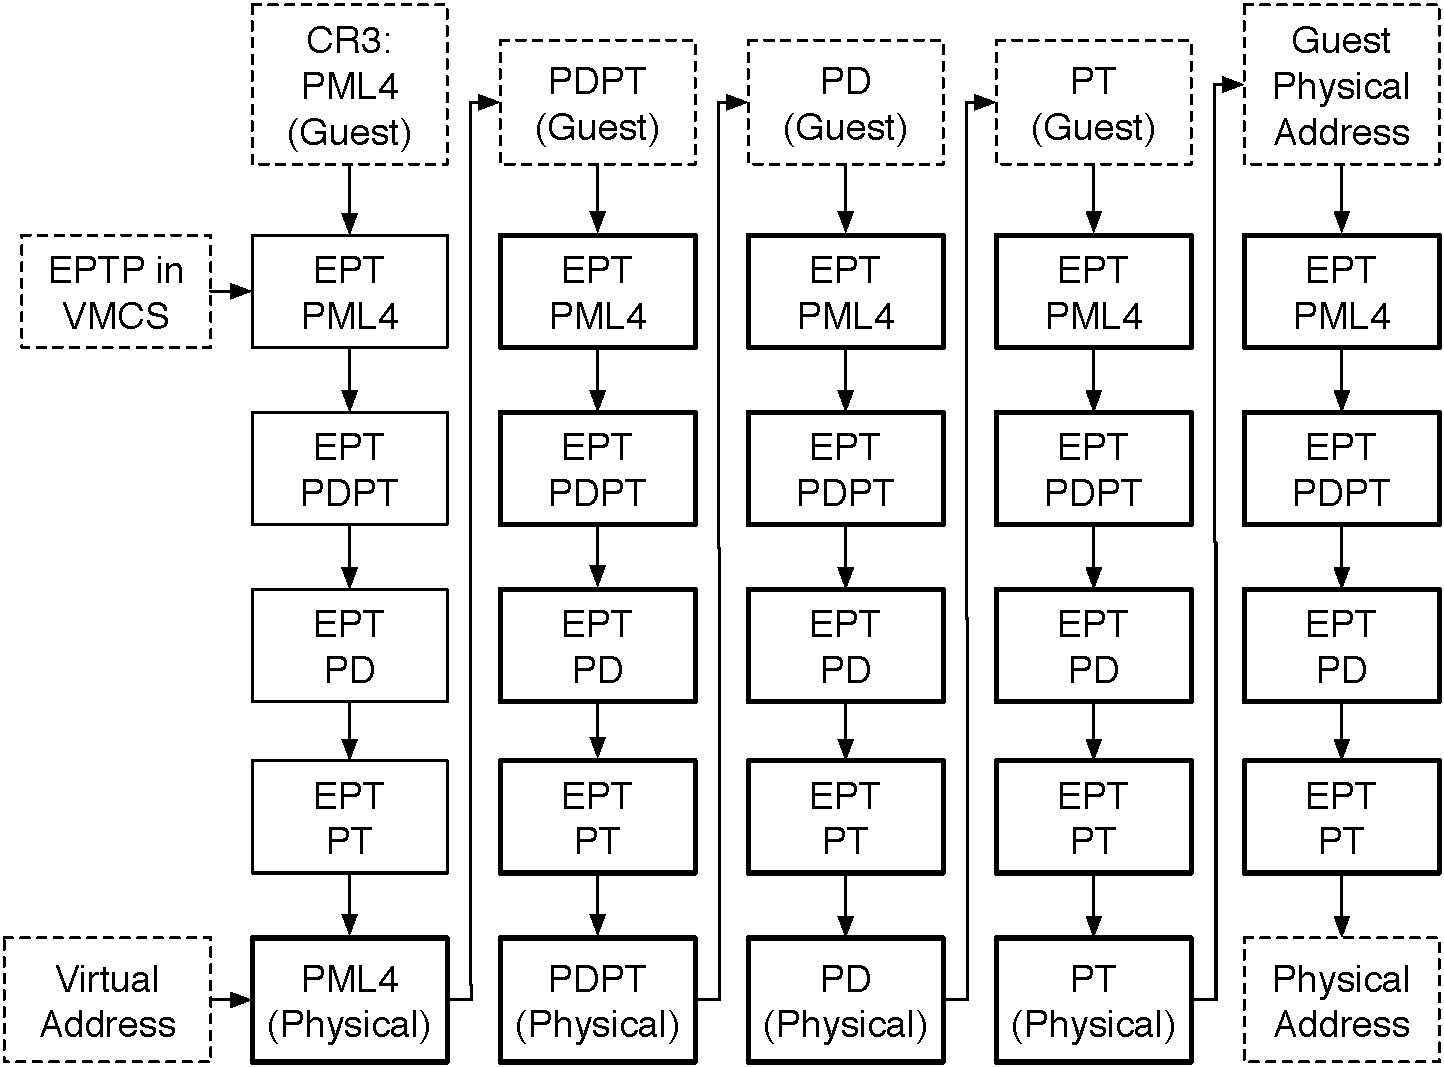
\includegraphics[width=85mm]{figures/vmx_paging.pdf}
  \caption{
    Address translation when hardware virtualization is enabled. The
    kernel-managed page tables contain guest-physical addresses, so each level
    in the kernel's page table requires a full walk of the hypervisor's
    extended page table~(EPT).  A translation requires up to 20 memory accesses
    (the bold boxes), assuming the physical address of the kernel's PML4 is
    cached.
  }
  \label{fig:vmx_paging}
\end{figure}


\HeadingLevelC{Page Table Attributes}
\label{sec:page_table_attributes}

Each page table entry contains a physical address, as shown in
Figure~\ref{fig:os_paging}, and some Boolean values that are referred to as
\textit{flags} or \textit{attributes}. The following attributes are used to
implement page swapping and software isolation.

The \textit{present}~(P) flag is set to 0 to indicate unused parts
of the address space, which do not have physical memory associated with them.
The system software also sets the P flag to 0 for pages that are evicted from
DRAM. When the address translation unit encounters a zero P flag, it aborts the
translation process and issues a hardware exception, as described in
\S~\ref{sec:faults}. This hardware exception gives system software an
opportunity to step in and bring an evicted page back into DRAM.

The \textit{accessed}~(A) flag is set to 1 by the CPU whenever the address
translation machinery reads a page table entry, and the \textit{dirty}~(D) flag
is set to 1 by the CPU when an entry is accessed by a memory write operation.
The A and D flags give the hypervisor and kernel insight into application
memory access patterns and inform the algorithms that select the pages that get
evicted from RAM.

% Page-Level Protection: SDM S 5.11, S 5.11.{1,2,3,4}

The main attributes supporting software isolation are the
\textit{writable}~(W) flag, which can be set to 0 to
prohibit\footnote{Writes to non-writable pages result in \#GP exceptions
(\S~\ref{sec:faults}).} writes to any memory location inside a page, the
\textit{disable execution}~(XD) flag, which can be set to 1 to prevent
instruction fetches from a page, and the \textit{supervisor}~(S) flag, which
can be set to 1 to prohibit any accesses from application software running at
ring 3.

\HeadingLevelB{Execution Contexts}
\label{sec:registers}

Application software targeting the 64-bit Intel architecture uses a variety of
CPU registers to interact with the processor's features, shown in
Figure~\ref{fig:cpu_registers} and Table~\ref{fig:xsave_state}. The values in
these registers make up an application thread's state, or \textit{execution
context}.

OS kernels multiplex each logical processor (\S~\ref{sec:cpu_core}) between
multiple software threads by \textit{context switching}, namely saving the
values of the registers that make up a thread's execution context, and
replacing them with another thread's previously saved context. Context
switching also plays a part in executing code inside secure containers, so its
design has security implications.

% 64-Bit Mode Execution Environment: SDM vol1 S 3.2.1
% Basic Program Execution Registers: SDM vol1 S 3.4

\begin{figure}[hbt]
  \centering
  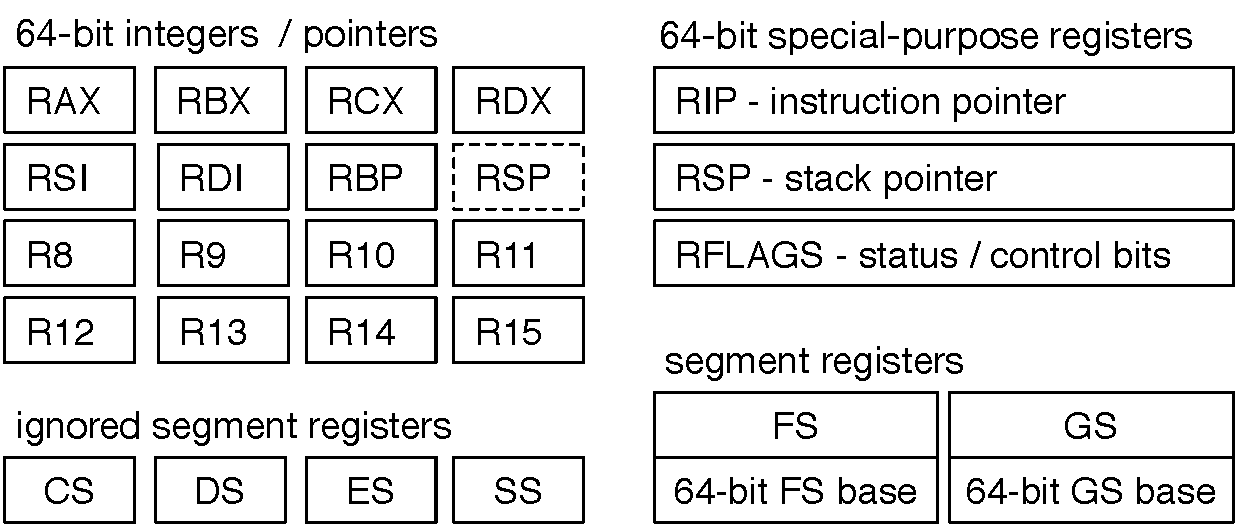
\includegraphics[width=85mm]{figures/cpu_registers.pdf}
  \caption{
    CPU registers in the 64-bit Intel architecture. RSP can be used as a
    general-purpose register (GPR), e.g., in pointer arithmetic, but it always
    points to the top of the program's stack. Segment registers are covered in
    \S~\ref{sec:segments}.
  }
  \label{fig:cpu_registers}
\end{figure}

Integers and memory addresses are stored in 16 \textit{general-purpose
registers} (GPRs). The first 8 GPRs have historical names: RAX, RBX, RCX,
RDX, RSI, RDI, RSP, and RBP, because they are extended versions of the 32-bit
Intel architecture's GPRs. The other 8 GPRs are simply known as R9-R16. RSP is
designated for pointing to the top of the procedure call stack, which is simply
referred to as \textit{the stack}. RSP and the stack that it refers to are
automatically read and modified by the CPU instructions that implement
procedure calls, such as \texttt{CALL} and \texttt{RET} (return), and by
specialized stack handling instructions such as \texttt{PUSH} and \texttt{POP}.

All applications also use the RIP register, which contains the address of the
currently executing instruction, and the RFLAGS register, whose bits (e.g.,
the carry flag - CF) are individually used to store comparison results and
control various instructions.

% XSAVE-Supported Features and State-Component Bitmaps: SDM vol1 S 13.1
% Enabling the XSAVE Feature Set and XSAVE-Enabled Features: SDM vol1 S13.3
% XSAVE-managed State: SDM vol1 S 13.5

Software might use other registers to interact with specific processor
features, some of which are shown in Table~\ref{fig:xsave_state}.

\begin{table}[hbt]
  \centering
  \begin{tabularx}{\columnwidth}{| l | X | l |}
  \hline
  \textbf{Feature} & \textbf{Registers} & \textbf{XCR0 bit}\\
  \hline
  FPU & FP0 - FP7, FSW, FTW & 0 \\
  \hline
  SSE & MM0 - MM7, XMM0 - XMM15, XMCSR & 1 \\
  \hline
  AVX & YMM0 - YMM15 & 2 \\
  \hline
  MPX & BND0 - BND 3 & 3 \\
  \hline
  MPX & BNDCFGU, BNDSTATUS & 4 \\
  \hline
  AVX-512 & K0 - K7 & 5 \\
  \hline
  AVX-512 & ZMM0\_H  - ZMM15\_H & 6 \\
  \hline
  AVX-512 & ZMM16 - ZMM31 & 7 \\
  \hline
  PK & PKRU & 9 \\
  \hline
  \end{tabularx}
  \caption{Sample feature-specific Intel architecture registers.}
  \label{fig:xsave_state}
\end{table}

The Intel architecture provides a future-proof method for an OS kernel to save
the values of feature-specific registers used by an application. The
\texttt{XSAVE} instruction takes in a \textit{requested-feature bitmap}~(RFBM),
and writes the registers used by the features whose RFBM bits are set to 1 in a
memory area. The memory area written by \texttt{XSAVE} can later be used by the
\texttt{XRSTOR} instruction to load the saved values back into feature-specific
registers. The memory area includes the RFBM given to \texttt{XSAVE}, so
\texttt{XRSTOR} does not require an RFBM input.

Application software declares the features that it plans to use to the kernel,
so the kernel knows what XSAVE bitmap to use when context-switching. When
receiving the system call, the kernel sets the XCR0 register to the feature
bitmap declared by the application. The CPU generates a fault if application
software attempts to use features that are not enabled by XCR0, so applications
cannot modify feature-specific registers that the kernel wouldn't take into
account when context-switching. The kernel can use the \texttt{CPUID}
instruction to learn the size of the \texttt{XSAVE} memory area for a given
feature bitmap, and compute how much memory it needs to allocate for the
context of each of the application's threads.

\subsection{Segment Registers}
\label{sec:segments}

The price of the Intel 64-bit architecture's widespread adoption was the
ability to run software targeting the older 32-bit architecture side-by-side
with 64-bit software \cite{cnet2005itanium}, which resulted in some warts in
the 64-bit architecture. While most warts are not material to the understanding
and operation of SGX, the 64-bit architecture's segment registers and vestigial
segmentation model must be understood. Therefore, this section covers the
segmentation concepts needed to understand SGX.

The semantics of the Intel architecture's instructions include the implicit use
of a few segments which are loaded into the processor's
\textit{segment registers} shown in Figure~\ref{fig:cpu_registers}. Code
fetches use the \textit{code segment} (CS).  Instructions that reference the
stack implicitly use the \textit{stack segment} (SS). Memory references
implicitly use the \textit{data segment} (DS) or the \textit{destination
segment} (ES). Via segment override prefixes, instructions can be modified to
use the unnamed segments FS and GS for memory references.

Modern operating systems effectively disable segmentation by covering the
entire addressable space with one segment, which is loaded in CS, and one data
segment, which is loaded in SS, DS and ES. The FS and GS registers store
segments covering \textit{thread-local storage} (TLS).

% Segment Selectors: SDM S 3.4.2
% Segment Registers: SDM S 3.4.3

Due to the Intel architecture's 16-bit origins, segment registers are exposed
as 16-bit values, called \textit{segment selectors}. The top 13 bits in a
selector are an index in a \textit{descriptor table}, and the bottom 2 bits are
the selector's ring number, which is also called requested privilege level
(RPL) in the Intel documentation. Also, modern system software only uses rings
0 and 3 (see \S~\ref{sec:rings}).

% Segment Loading Instructions in IA-32e Mode: SDM S 3.4.4
% Limit Checking in 64-bit Mode: SDM S 5.3.1
% Privilege Levels: SDM S 5.5

Each segment register has a hidden \textit{segment descriptor}, which consists
of a \textit{base address}, \textit{limit}, and type information, such as
whether the descriptor should be used for executable code or data.
Figure~\ref{fig:cpu_segment} shows the effect of loading a 16-bit selector into
a segment register. The selector's index is used to read a descriptor from the
descriptor table and copy it into the segment register's hidden descriptor.

\begin{figure}[hbt]
  \center{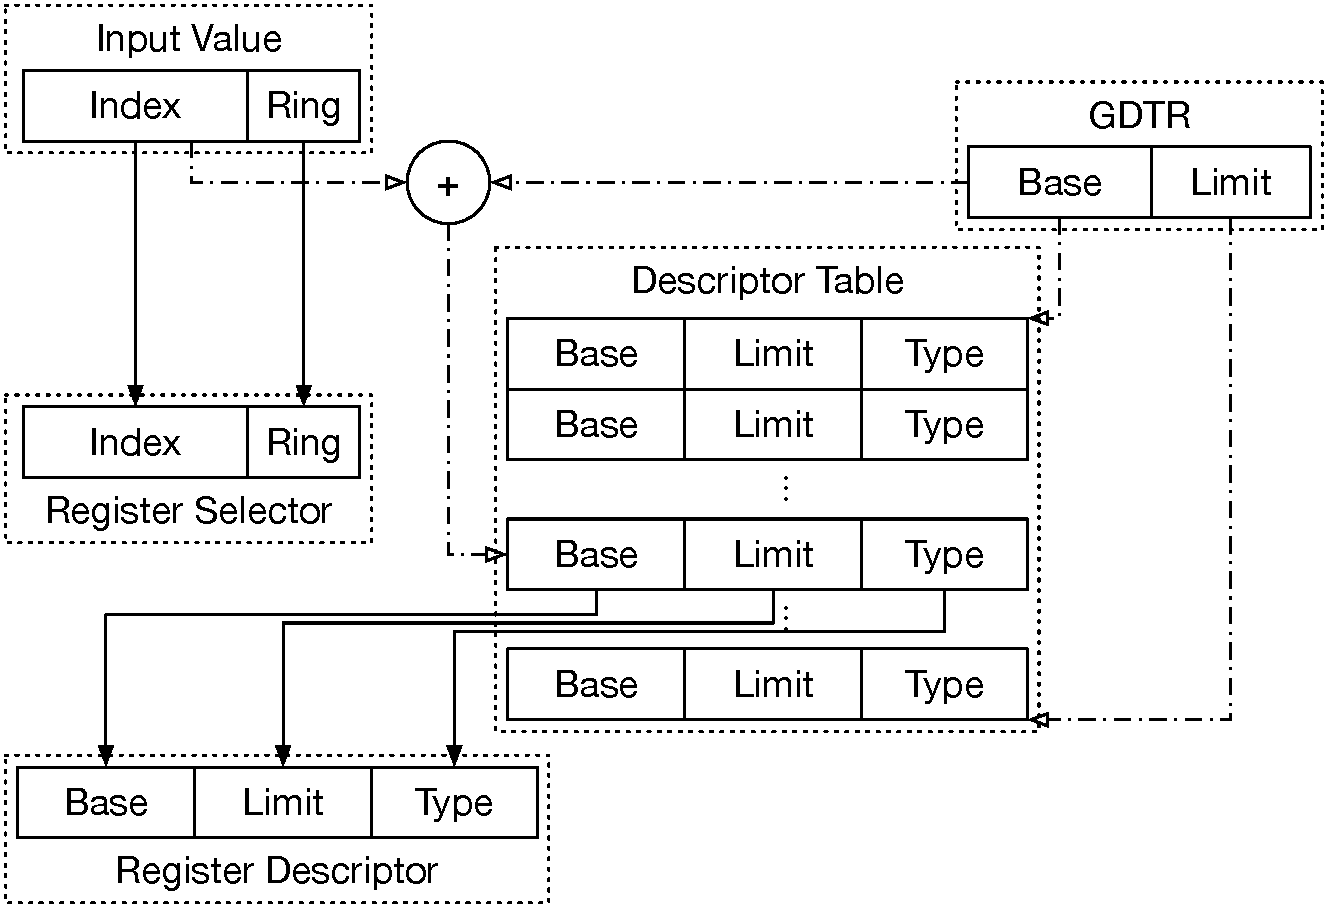
\includegraphics[width=85mm]{figures/cpu_segment.pdf}}
  \caption{
    Loading a segment register. The 16-bit value loaded by software is a
    selector consisting of an index and a ring number. The index selects a GDT
    entry, which is loaded into the descriptor part of the segment register.
  }
  \label{fig:cpu_segment}
\end{figure}

In 64-bit mode, all segment limits are ignored. The base addresses in most
segment registers (CS, DS, ES, SS) are ignored. The base addresses in FS and GS
are used, in order to support thread-local storage.
Figure~\ref{fig:cpu_segmentation} outlines the address computation in this
case. The instruction's address, named \textit{logical address} in the Intel
documentation, is added to the base address in the segment register's
descriptor, yielding the virtual address, also named \textit{linear address}.
The virtual address is then translated (\S~\ref{sec:paging}) to a physical
address.

\begin{figure}[hbt]
  \center{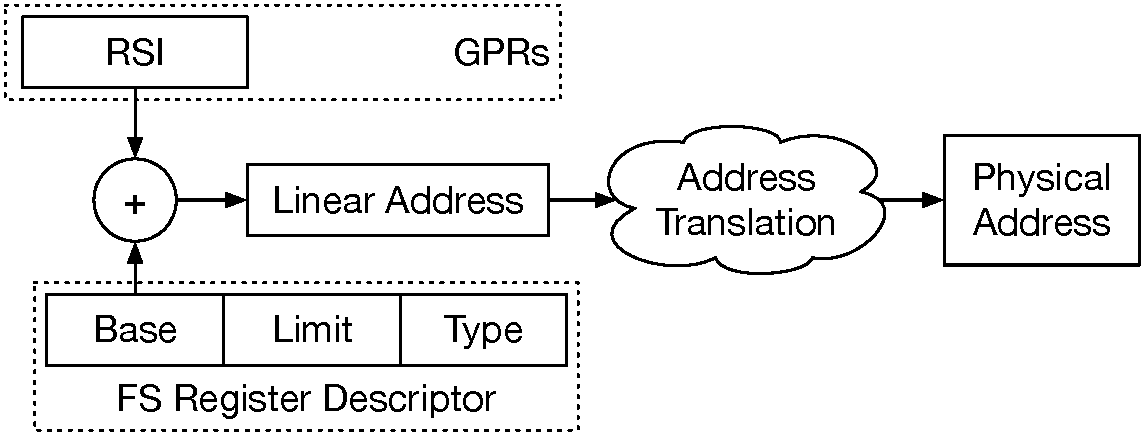
\includegraphics[width=80mm]{figures/cpu_segmentation.pdf}}
  \caption{
    Example address computation process for \texttt{MOV FS:[RDX], 0}.  The
    segment's base address is added to the address in RDX before address
    translation (\S~\ref{sec:paging}) takes place.
  }
  \label{fig:cpu_segmentation}
\end{figure}

Outside the special case of using FS or GS to reference thread-local storage,
the logical and virtual (linear) addresses match, so most of this paper uses
the term ``virtual address'' and ignores segmentation.

Even though CS is not used for segmentation, 64-bit system software needs to
load a valid selector into it. The CPU uses the ring number in the CS selector
to track the current privilege level, and uses one of the type bits to know
whether it's running 64-bit code, or 32-bit code in compatibility mode.

% Null Segment Selector Checking: SDM S 5.4.1, S 5.4.1.1

The DS and ES segment registers are completely ignored, and can have null
selectors loaded in them. The CPU loads a null selector in SS when switching
privilege levels, discussed in \S~\ref{sec:faults}.

% Segment Loading Instructions in IA-32e Mode: SDM S 3.4.4
% Segmentation in IA-32e Mode: SDM S 3.2.4

Modern kernels only use one descriptor table, the \textit{Global Descriptor
Table} (GDT), whose virtual address is stored in the GDTR register. Table~
\ref{fig:gdt_layout} shows a typical GDT layout that can be used by 64-bit
kernels to run both 32-bit and 64-bit applications.

\begin{table}[hbt]
  \center{\begin{tabular}{| l | l |}
  \hline
  \textbf{Descriptor} & \textbf{Selector}\\
  \hline
  Null (must be unused) & 0 \\
  \hline
  Kernel code & 0x08 (index 1, ring 0) \\
  \hline
  Kernel data & 0x10 (index 2, ring 0) \\
  \hline
  User code & 0x1B (index 3, ring 3) \\
  \hline
  User data & 0x1F (index 4, ring 3) \\
  \hline
  TSS & 0x20 (index 5, ring 0) \\
  \hline
  \end{tabular}}
  \caption{
    A typical GDT layout in the 64-bit Intel Architecture.
  }
  \label{fig:gdt_layout}
\end{table}

% TSS Descriptor: SDM S 7.2.2
% TSS Descriptor in 64-bit mode: SDM S 7.2.3
% Task Register: SDM S 7.2.4
% Task Management in 64-bit Mode: SDM S 7.7

The last entry in Table~\ref{fig:gdt_layout} is a descriptor for the
\textit{Task State Segment} (TSS), which was designed to implement hardware
context switching, named \textit{task switching} in the Intel documentation.
The descriptor is stored in the \textit{Task Register} (TR), which behaves like
the other segment registers described above.

Task switching was removed from the 64-bit architecture, but the TR segment
register was preserved, and it points to a repurposed TSS data structure. The
64-bit TSS contains an \textit{I/O map}, which indicates what parts of the I/O
address space can be accessed directly from ring 3, and the
\textit{Interrupt Stack Table} (IST), which is used for privilege level
switching (\S~\ref{sec:faults}).

Modern operating systems do not allow application software any direct access to
the I/O address space, so the kernel sets up a single TSS that is loaded into
TR during early initialization, and used to represent all applications running
under the OS.

\subsection{Privilege Level Switching}
\label{sec:privilege_switches}

Applications software needs a method to invoke the kernel, because it cannot
directly perform privileged operations, such as network or disk I/O. At the
same time, ring 3 software cannot be offered the ability to jump arbitrarily
into kernel code, as that would compromise the kernel's ability to isolate
applications and enforce security invariants.\footnote{For example, when an
application wishes to write a file to the disk, the kernel must check if the
application's user has access to that file. If the ring 3 code could perform
an arbitrary jump in kernel space, it would be able to skip the access check.}
Therefore, the processor has designated methods for switching privilege levels,
which protect the integrity of the privileged software.

This section describes the privilege switching mechanisms that impact the SGX
design, summarized in Figure~\ref{fig:cpu_ring_switch}. Also, understanding the
considerations behind privilege switching is useful when analyzing SGX, because
the process of calling code inside an enclave is similar to switching privilege
levels, as an enclave's code must be able to enforce its own security
invariants, just like an OS kernel.


\subsubsection{System Calls}
\label{sec:syscalls}

% Fast System Calls in 64-Bit Mode: SDM S 5.8.8

\begin{figure}[hbt]
  \center{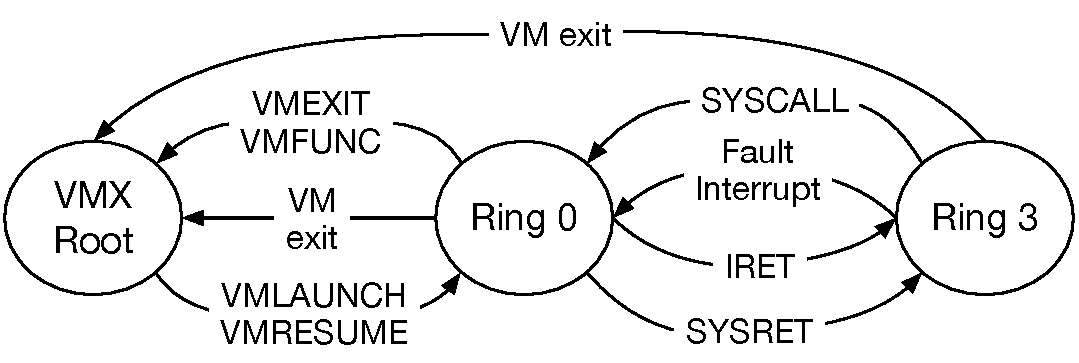
\includegraphics[width=85mm]{figures/cpu_ring_switch.pdf}}
  \caption{
    Modern privilege switching methods in the 64-bit Intel architecture.
  }
  \label{fig:cpu_ring_switch}
\end{figure}

On modern processors, application software uses the SYSCALL instruction to
invoke ring 0 code, and the kernel uses SYSRET to switch the privilege level
back to ring 3. SYSCALL jumps into a predefined kernel location, which is
specified by writing to a pair of architectural MSRs
(\S~\ref{sec:address_spaces}).  MSRs can only be read or written by ring 0
code, so application software cannot modify SYSCALL's MSRs and abuse the
SYSCALL instruction to execute arbitrary kernel code. The SYSRET instruction
switches back to ring 3 and jumps to the address in RCX, which is set by the
SYSCALL instruction. The SYSCALL / SYSRET pair is optimized for speed by
avoiding memory accesses. The design can get away without referencing a stack
because kernel calls are not recursive.


\subsubsection{Faults}
\label{sec:faults}

% Interrupt and Exception Handling: SDM S 6.1, S 6.2
% Access Rights: SDM S 4.6
% Page-Fault Exceptions: SDM S 4.7

The processor also performs a switch from ring 3 to ring 0 when a \textit{
hardware exception} occurs while executing application code. Some exceptions
indicate bugs in the application, whereas other exceptions require kernel
action. A \textit{general protection fault} (\#GP) occurs when software
attempts to perform a disallowed action, such as setting the CR3 register from
ring 3. A \textit{page fault} (\#PF) occurs when address translation encounters
a page table entry whose P flag is 0, or attempting to use a page in a way
inconsistent with the access bits in its page table entry, for example
accessing a page whose S bit is set from ring 3.

% Interrupt Descriptor Table (IDT): SDM S 6.10

When a hardware exception occurs in application code, the CPU performs a ring
switch, and calls the corresponding \textit{exception handler}. For example,
the \#GP handler typically terminates the application's process, while the \#PF
handler reads the swapped out page back into RAM and resumes the application's
execution.

The exception handlers are a part of the OS kernel, and their locations are
specified in the first 32 entries of the Interrupt Descriptor Table (IDT),
whose structure is shown in Table~\ref{fig:idt_entry}. The IDT's physical
address is stored in the IDTR register, which can only be accessed by ring 0
code. Kernels protect the IDT memory using page tables, so that ring 3 software
cannot access it.

\begin{table}[hbt]
  \center{\begin{tabular}{| l | r |}
  \hline
  \textbf{Field} & \textbf{Bits} \\
  \hline
  Handler RIP & 64 \\
  \hline
  Handler CS & 16 \\
  \hline
  Interrupt Stack Table (IST) index & 3 \\
  \hline
  \end{tabular}}
  \caption{
    The essential fields of an IDT entry in 64-bit mode. Each entry points to a
    hardware exception or interrupt handler.
  }
  \label{fig:idt_entry}
\end{table}

Each IDT entry has a 3-bit index pointing into the Interrupt Stack Table (IST),
which is an array of 8 stack pointers stored in the TSS described in
\S~\ref{sec:segments}.

% 64-Bit Mode Stack Frame: SDM S 6.14.2
% IRET in IA-32e Mode: SDM S 6.14.3
% Stack Switching in IA-32e Mode: SDM S 6.14.4
% Interrupt Stack Table: SDM S 6.14.5

When a hardware exception occurs, the execution state may be corrupted, and the
current stack cannot be relied on. Therefore, the CPU first uses the handler's
IDT entry to set up a known good stack. SS is loaded with a null descriptor,
and RSP is set to the IST value pointed by the IDT entry. After switching to a
reliable stack, the CPU pushes the snapshot in Table~\ref{fig:fault_stack} on
the stack, then loads the IDT entry's values into the CS and RIP registers,
which trigger the execution of the exception handler.

\begin{table}[hbt]
  \center{\begin{tabular}{| l | r |}
  \hline
  \textbf{Field} & \textbf{Bits} \\
  \hline
  Exception SS & 64 \\
  \hline
  Exception RSP & 64 \\
  \hline
  RFLAGS & 64 \\
  \hline
  Exception CS & 64 \\
  \hline
  Exception RIP & 64 \\
  \hline
  Exception code & 64 \\
  \hline
  \end{tabular}}
  \caption{
    The snapshot pushed on the handler's stack when a hardware exception
    occurs. IRET restores registers from this snapshot.
  }
  \label{fig:fault_stack}
\end{table}

After the exception handler completes, it uses the \texttt{IRET} (interrupt
return) instruction to load the registers from the on-stack snapshot and switch
back to ring 3.

The Intel architecture gives the fault handler complete control over the parts
of the execution context not listed in Table~\ref{fig:fault_stack}. This
privilege is used by some handlers (e.g., \#GP) to perform context switches
(\S~\ref{sec:registers}) after a process is terminated due to a bug. However,
in the SGX threat model, system software is not trusted, and giving it access
to an enclave's execution context would expose potentially sensitive
information, and present an opportunity to compromise the enclave's integrity.
Therefore, SGX cannot use the current fault handling process, and must modify
it.


\subsubsection{VM Exits}
\label{sec:vm_exits}

If an EPT entry has the P flag set to 0, the CPU performs a VM exit, and the
hypervisor has an opportunity to bring the page into RAM.






\subsection{A Computer Map}

This section maps out a computer using the Intel architecture at three zoom
levels: the motherboard, the CPU, and the execution core, focusing on the
concepts needed to understand SGX and analyze its security properties. Most
details in here are documented in Intel's
\textit{Optimization Reference Manual} \cite{intel2014optimization}.


\subsubsection{The Motherboard}
\label{sec:motherboard}

A computer's components are connected by a printed circuit board called a
\textit{motherboard}, which consists of \textit{sockets} connected by
\textit{buses}. Sockets connect chip-carrying \textit{packages} to the board.
The Intel documentation uses the term ``package'' to specifically refer to a
CPU.

The buses most relevant to SGX (see Figure~\ref{fig:motherboard}) are the
\textit{Quick-Path Interconnect} (QPI) \cite{intel2009qpi}, a network of
point-to-point links that connect processors, the \textit{double data rate}
(DDR) bus that connects a CPU to DRAM, and the \textit{Peripheral Component
Interconnect Express} (PCIe) bus that connects a CPU to peripherals such as a
\textit{Network Interface Card} (NIC).

\begin{figure}[hbt]
  \center{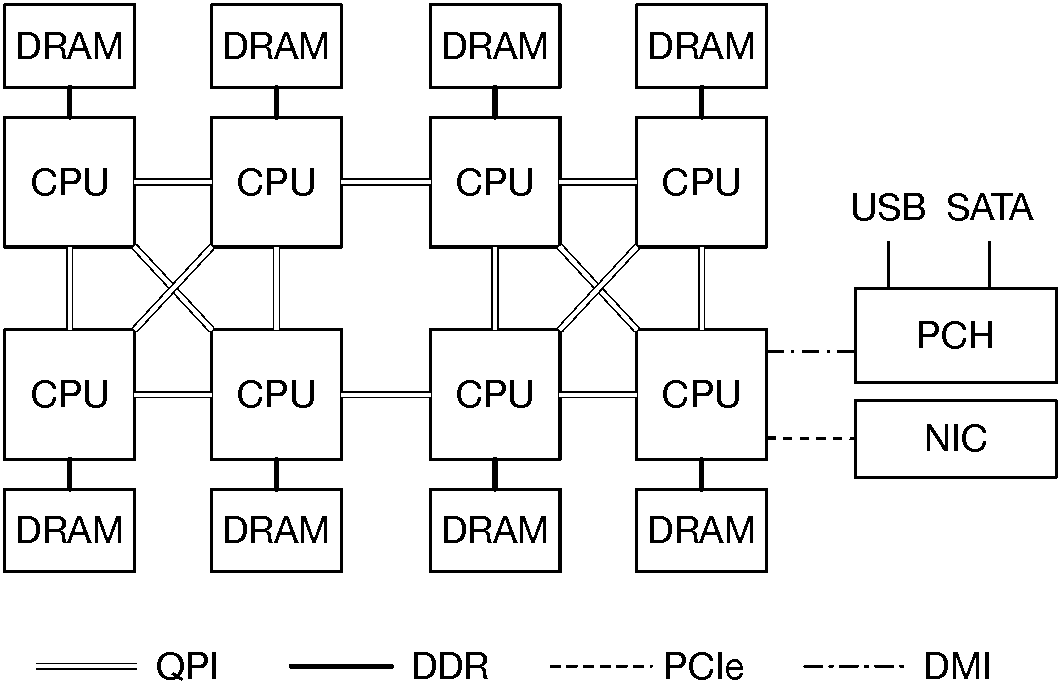
\includegraphics[width=85mm]{figures/motherboard.pdf}}
  \caption{
    The motherboard structures that are most relevant to SGX.
  }
  \label{fig:motherboard}
\end{figure}

The SGX trusted computing base includes the processor package, and excludes the
other hardware in the computer. It follows that SGX must be able to fend off
attacks from rogue devices, such as the PCIe NIC used to compromise Intel TXT
\cite{wojtczuk2011txt}, as well as passive or active bus-tapping attacks, such
as the memory bus tap used to hack the Xbox \cite{huang2003xbox} and the
memory glitching attack that subverted the PlayStation 3 hypervisor
\cite{hotz2010ps3}.


\subsubsection{The Processor}
\label{sec:cpu_die}

An Intel processor's die, illustrated in Figure~\ref{fig:cpu_die}, is divided
into two broad areas: the \textit{core area} implements the instruction
execution pipeline typically associated with CPUs, while the \textit{uncore}
provides functions that were traditionally hosted on separate chips, but are
currently integrated on the CPU die to save power and improve latency.

\begin{figure}[hbt]
  \center{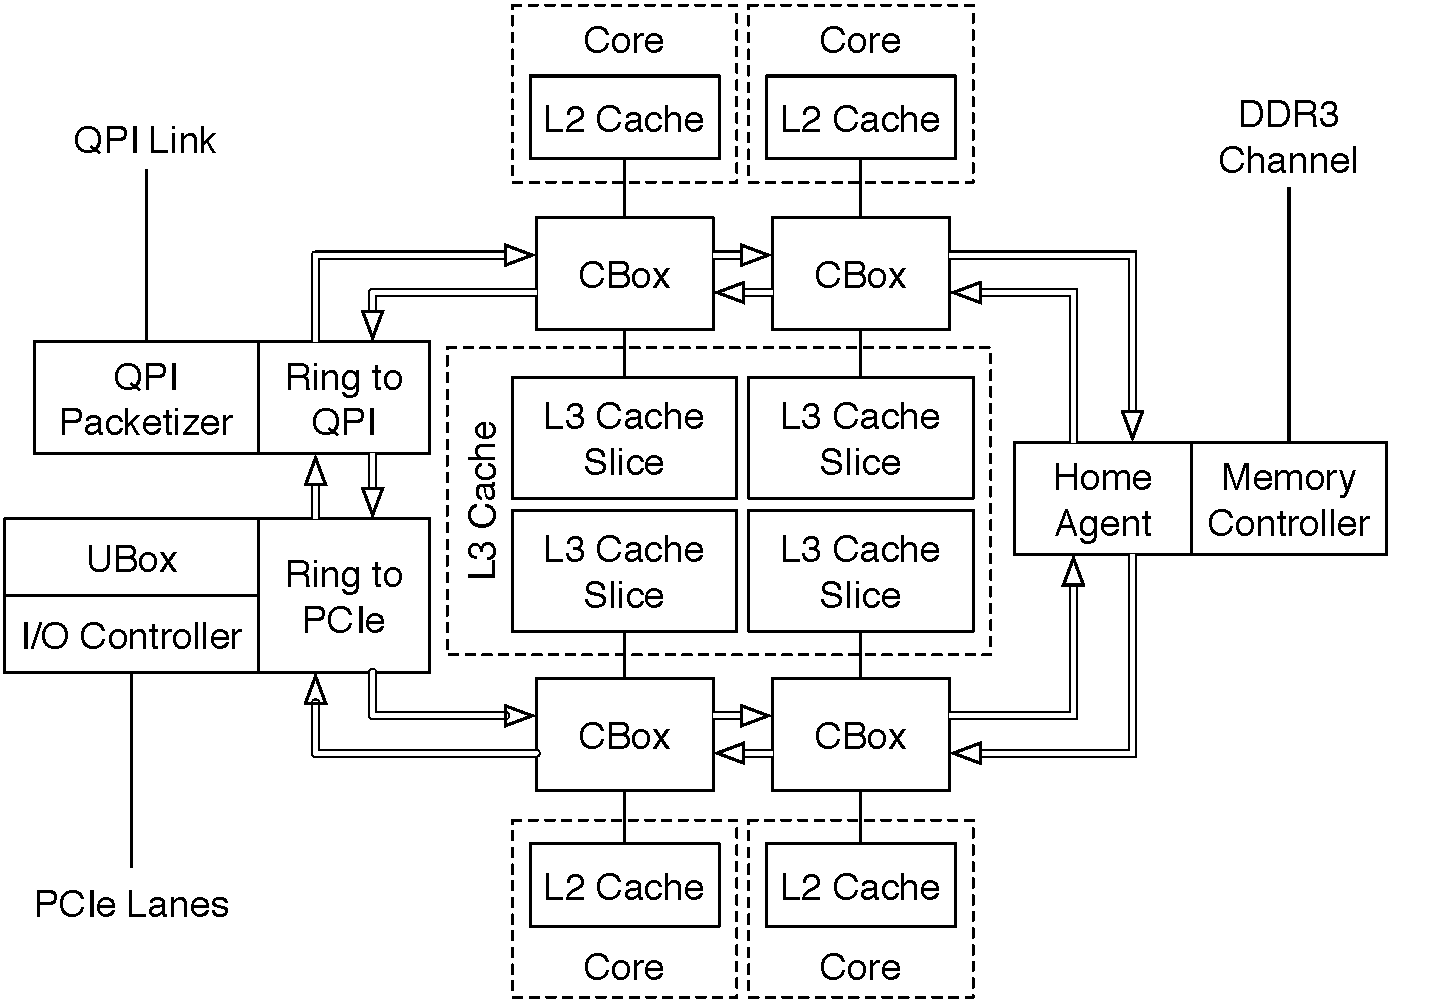
\includegraphics[width=85mm]{figures/cpu_die.pdf}}
  \caption{
    The major components in a modern CPU package. \S~\ref{sec:cpu_die} gives
    an uncore overview. \S~\ref{sec:cpu_core} describes execution cores.
    \S~\ref{sec:cache_coherence} takes a deeper look at the uncore.
  }
  \label{fig:cpu_die}
\end{figure}

% Ring Interconnect and Last Level Cache: Optimization S 2.2.5.3
% System Agent: Optimization S 2.2.6

At a conceptual level, the uncore of modern processors includes a memory
controller that interfaces with the DDR bus, an I/O controller that can
arbitrate the PCIe bus, and a growing number of integrated controllers for
peripherals, such as a NIC and a GPU. The uncore structure is described in some
processor family datasheets \cite{intel2014datasheet, intel2010datasheet}, and
in the overview sections in Intel's uncore performance monitoring documentation
\cite{intel2014uncore, intel2012uncore, intel2010uncore}.

The SGX design relies on the fact that the processor die includes the memory
and I/O controller, and thus can prevent any device from accessing protected
memory areas via \textit{Direct Memory Access} (DMA) transfers.
\S~\ref{sec:cache_coherence} takes a deeper look at the uncore organization and
at the mechanism used by the SGX implementation to protect sensitive memory.


\subsubsection{The Core}
\label{sec:cpu_core}

Virtually all modern Intel processors have core areas consisting of multiple
copies of the execution core circuitry, each of which is called a
\textit{core}.  At the time of this writing, desktop-class Intel CPUs have 4
cores, and server-class CPUs have as many as 18 cores.

Most Intel CPUs feature \textit{hyper-threading}, which means that a core
(shown in Figure~\ref{fig:cpu_core}) has two copies of the register files
backing the execution context described in \S~\ref{sec:registers}, and can
execute two separate streams of instructions simultaneously. Hyper-threading
increases the utilization of the shared fetch, decode and execution units, in
the presence of memory stalls.

\begin{figure}[hbt]
  \center{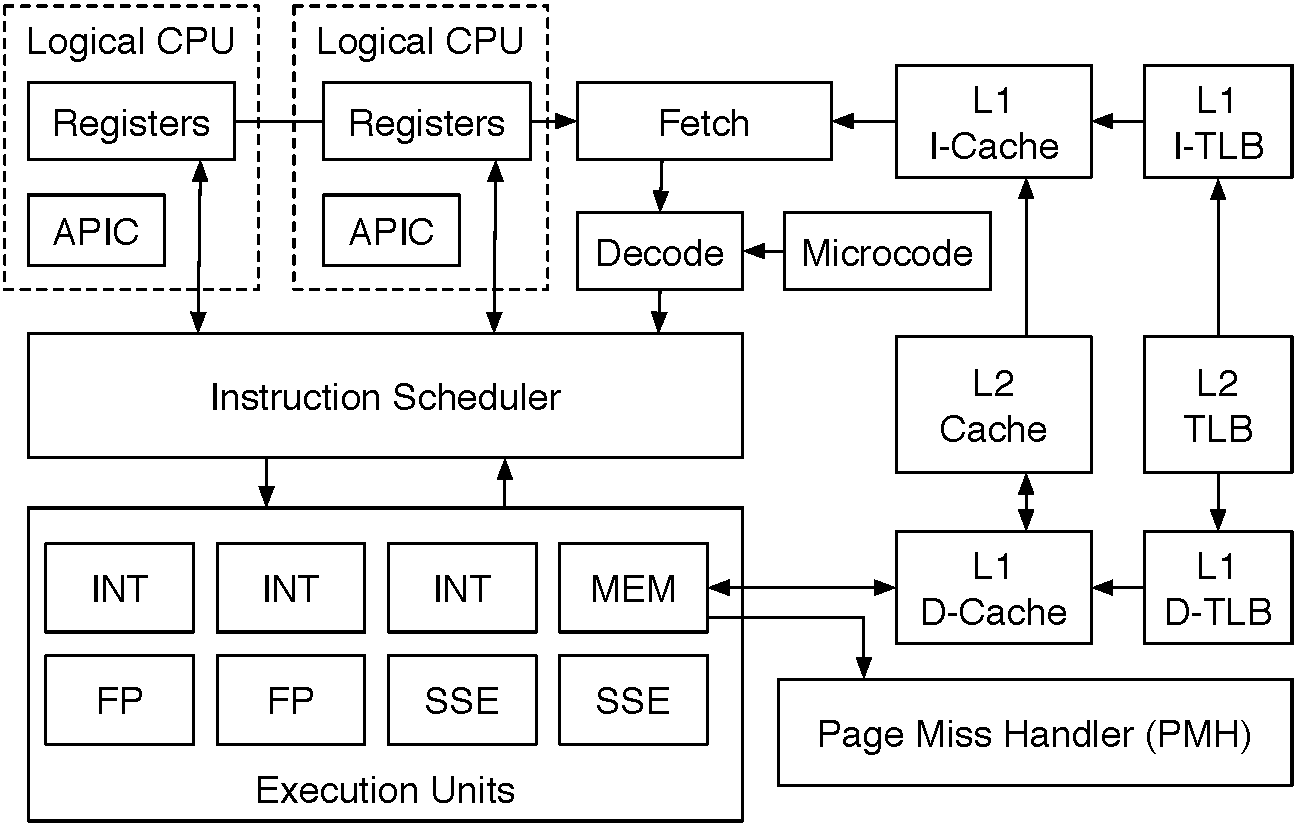
\includegraphics[width=85mm]{figures/cpu_core.pdf}}
  \caption{
    CPU core with two logical processors. Each logical processor has its own
    execution context and local APIC, and they share all the other core
    resources.
  }
  \label{fig:cpu_core}
\end{figure}

A hyper-threaded core is exposed to system software as two \textit{logical
processors}, also named \textit{hardware threads} in the Intel documentation.
The logical processor abstraction allows the code used to distribute work
across processors in a multi-processor system to function without any change on
multi-core hyper-threaded processors.

The high level of resource sharing introduced by hyper-threading introduces a
security vulnerability. Software running on one logical processor can use the
high-performance counter \cite{petters1999making} to get information about the
instructions and memory access patterns of another piece of software that is
executed on the other logical processor in the same core.

\subsection{Out-of-Order and Speculative Execution}
\label{sec:out_of_order}

% Outcome: distinguish observed execution order from program order

CPU cores can execute instructions orders of magnitude faster than DRAM can
read data. Computer architects attempt to bridge this gap by using
hyper-threading (\S~\ref{sec:cpu_die}), out-of-order and speculative execution,
and caching, which is described in \S~\ref{sec:caching}. In CPUs that use
out-of-order execution, the order in which the CPU carries out a program's
instructions (\textit{execution order}) is not necessarily the same as the
order in which the instructions would be executed by a sequential evaluation
system (\textit{program order}).

An analysis of a system's information leakage must take out-of-order execution
into consideration. Any CPU actions observed by an attacker match the execution
order, so the attacker may learn some information by comparing the observed
execution order with a known program order. At the same time, attacks that try
to infer a victim's program order based on actions taken by the CPU must
account for out-of-order execution as a source of noise.

This section summarizes the out-of-order and speculative execution concepts
used when reasoning about a system's security properties.
\cite{patterson2013architecture} and \cite{hennessy2012architecture} cover the
concepts in great depth, while Intel's optimization manual
\cite{intel2014optimization} provides details specific to Intel CPUs.

% The Haswell Microarchitecture: Optimization S 2.1

Figure~\ref{fig:cpu_out_of_order} provides a more detailed view of the CPU core
components involved in out-of-order execution, and omits some less relevant
details from Figure~\ref{fig:cpu_core}.

\begin{figure}[hbt]
  \centering
  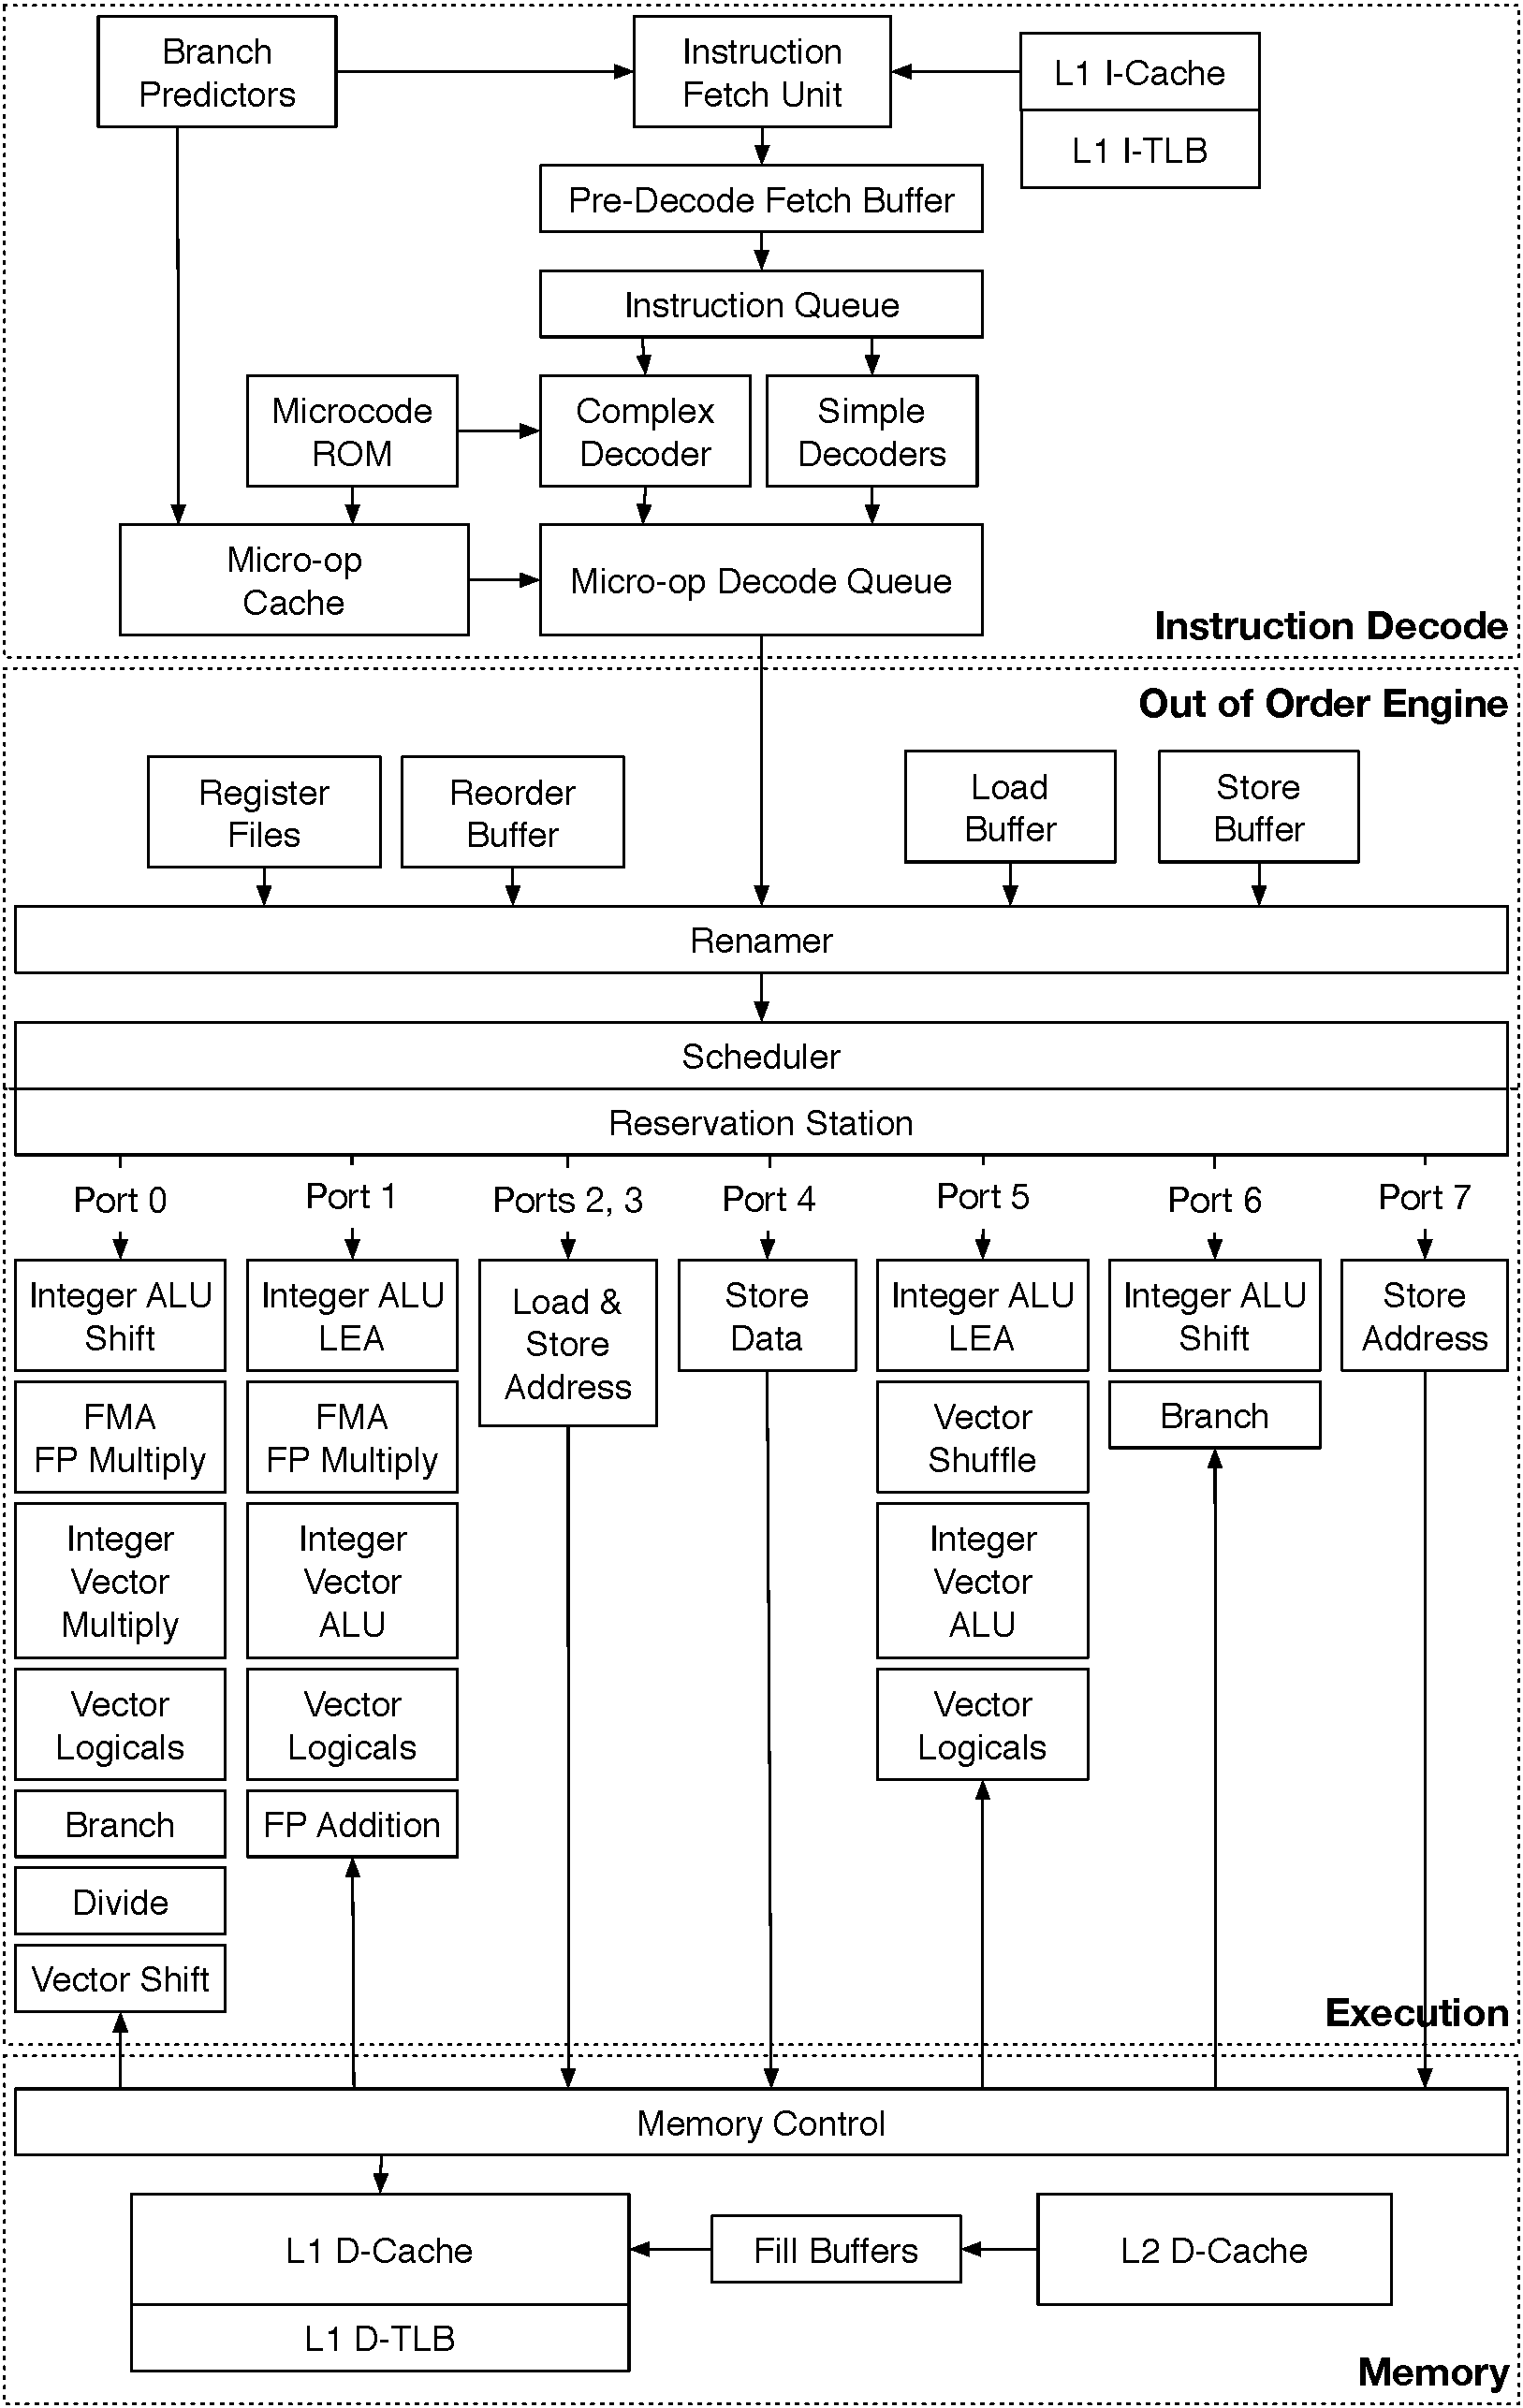
\includegraphics[width=87mm]{figures/cpu_out_of_order.pdf}
  \caption{
    The structures in a CPU core that are relevant to out-of-order and
    speculative execution. Instructions are decoded into micro-ops, which are
    scheduled on one of the execution unit's ports. The branch predictor
    enables speculative execution when a branch is encountered.
  }
  \label{fig:cpu_out_of_order}
\end{figure}

% Intel Microarchitecture Code Name Sandy Bridge Pipeline Overview:
%     Optimization S 2.2.1
% The Front End: Optimization S 2.2.2

The Intel architecture defines a \textit{complex instruction set} (CISC).
However, virtually all modern CPUs are architected following \textit{reduced
instruction set} (RISC) principles. This is accomplished by having the
instruction decode stages break down each instruction into \textit{micro-ops},
which resemble RISC instructions. The other stages of the execution pipeline
work exclusively with micro-ops.


\subsubsection{Out-of-Order Execution}

% Out of Order Engine: Optimization S 2.2.23
% The Execution Core: S 2.2.4

Different types of instructions require different logic circuits, called
\textit{functional units}. For example, the arithmetic logic unit (ALU), which
performs arithmetic operations, is completely different from the load store
unit, which peforms memory operations. Different circuits can be used at the
same time, so each CPU core can execute multiple micro-ops in parallel.

The core's out-of-order engine receives decoded micro-ops, identifies the
micro-ops that can execute in parallel, assigns them to functional units, and
combines the outputs of the units so that the results are equivalent to having
the micro-ops executed sequentially in the order in which they come from the
decode stages.

For example, consider the sequence of pseudo micro-ops\footnote{The set of
micro-ops used by Intel CPUs is not publicly documented. The fictional examples
in this section suffice for illustration purposes.} in
Table~\ref{fig:out_of_order_micro_ops} below. The \texttt{OR} uses the result
of the \texttt{LOAD}, but the \texttt{ADD} does not. Therefore, a good
scheduler can have the load store unit execute the \texttt{LOAD} and the ALU
execute the \texttt{ADD}, all in the same clock cycle.

\begin{table}[hbt]
  \centering
  \begin{tabular}{| l | l | l |}
  \hline
  \textbf{\#} & \textbf{Micro-op} & \textbf{Meaning}\\
  \hline
  1 & \texttt{LOAD RAX, RSI} & RAX $\leftarrow$ DRAM[RSI]\\
  \hline
  2 & \texttt{OR RDI, RDI, RAX} & RDI $\leftarrow$ RDI $\lor$ RAX\\
  \hline
  3 & \texttt{ADD RSI, RSI, RCX} & RSI $\leftarrow$ RSI + RCX\\
  \hline
  4 & \texttt{SUB RBX, RSI, RDX} & RBX $\leftarrow$ RSI - RDX\\
  \hline
  \end{tabular}
  \caption{
    Pseudo micro-ops for the out-of-order execution example.
  }
  \label{fig:out_of_order_micro_ops}
\end{table}

% Renamer: Optimization S 2.2.3.1

The out-of-order engine in recent Intel CPUs works roughly as follows.
Micro-ops received from the decode queue are written into a \textit{reorder
buffer} (ROB) while they are \textit{in-flight} in the execution unit. The
\textit{register allocation table} (RAT) matches each register with the last
reorder buffer entry that updates it. The \textit{renamer} uses the RAT to
rewrite the source and destination fields of micro-ops when they are written in
the ROB, as illustrated in Tables \ref{fig:out_of_order_rob} and
\ref{fig:out_of_order_rat}. Note that the ROB representation makes it easy to
determine the dependencies between micro-ops.

\begin{table}[hbt]
  \centering
  \begin{tabular}{| l | l | l | l | l |}
  \hline
  \textbf{\#} & \textbf{Op} & \textbf{Source 1} & \textbf{Source 2} &
  \textbf{Destination}\\
  \hline
  1 & LOAD & RSI & $\emptyset$ & RAX \\
  \hline
  2 & OR & RDI & ROB \#1 & RSI \\
  \hline
  3 & ADD & RSI & RCX & RSI \\
  \hline
  4 & SUB & ROB \# 3 & RDX & RBX \\
  \hline
  \end{tabular}
  \caption{
    Data written by the renamer into the reorder buffer (ROB), for the
    micro-ops in Table~\ref{fig:out_of_order_micro_ops}.
  }
  \label{fig:out_of_order_rob}
\end{table}

\begin{table}[hbt]
  \centering
  \begin{tabular}{| l | r | r | r | r | r | r |}
  \hline
  \textbf{Register} & RAX & RBX & RCX & RDX & RSI & RDI \\
  \hline
  \textbf{ROB \#} & \#1 & \#4 & $\emptyset$ & $\emptyset$ & \#3 & \#2 \\
  \hline
  \end{tabular}
  \caption{
    Relevant entries of the register allocation table after the micro-ops in
    Table~\ref{fig:out_of_order_micro_ops} are inserted into the ROB.
  }
  \label{fig:out_of_order_rat}
\end{table}

% Scheduler: Optimization S 2.2.3.2

The scheduler decides which micro-ops in the ROB get executed, and places them
in the \textit{reservation station}. The reservation station has one port
for each functional unit that can execute micro-ops independently. Each
reservation station port port holds one micro-op from the ROB. The reservation
station port waits until the micro-op's dependencies are satisfied and forwards
the micro-op to the functional unit. When the functional unit completes
executing the micro-op, its result is \textit{written back} to the ROB, and
forwarded to any other reservation station port that depends on it.

The ROB stores the results of completed micro-ops until they are
\textit{retired}, meaning that the results are \textit{committed} to the
register file and the micro-ops are removed from the ROB. Although micro-ops
can be executed out-of-order, they must be retired in program order, in order
to handle exceptions correctly. When a micro-op causes a hardware exception
(\S~\ref{sec:faults}), all the following micro-ops in the ROB are
\textit{squashed}, and their results are discarded.

In the example above, the \texttt{ADD} can complete before the \texttt{LOAD},
because it does not require a memory access. However, the \textit{ADD}'s result
cannot be committed before \texttt{LOAD} completes. Otherwise, if the
\textit{ADD} is committed and the \textit{LOAD} causes a page fault, software
will observe an incorrect value for the  RSI register.

% Load and Store Operation Overview: Optimization S 2.2.5

The ROB is tailored for discovering register dependencies between micro-ops.
However, micro-ops that execute out-of-order can also have memory dependencies.
For this reason, out-of-order engines have a \textit{load buffer} and a
\textit{store buffer} that keep track of in-flight memory operations and are
used to resolve memory dependencies.


\subsubsection{Speculative Execution}

% Branch Prediction: Optimization S 2.2.2.3

Branch instructions, also called \textit{branches}, change the instruction
pointer (RIP, \S~\ref{sec:registers}), if a condition is met (\textit{the
branch is taken}). They implement conditional statements (\texttt{if}) and
looping statements, such as \texttt{while} and \texttt{for}. The most
well-known branching instructions in the Intel architecture are in the
\texttt{j\textit{cc}} family, such as \texttt{je} (jump if equal).

Branches pose a challenge to the decode stage, because the instruction that
should be fetched after a branch is not known until the branching condition is
evaluated. In order to avoid stalling the decode stage, modern CPU designs
include \textit{branch predictors} that use historical information to guess
whether a branch will be taken or not.

When the decode stage encounters a branch instruction, it asks the branch
predictor for a guess as to whether the branch will be taken or not. The
decode stage bundles the branch condition and the predictor's guess into a
branch check micro-op, and then continues decoding on the path indicated by the
predictor. The micro-ops following the branch check are marked as
\textit{speculative}.

When the branch check micro-op is executed, the branch unit checks whether the
branch predictor's guess was correct. If that is the case, the branch check is
retired successfully. The scheduler handles \textit{mispredictions} by
squashing all the micro-ops following the branch check, and by signaling the
instruction decoder to flush the micro-op decode queue and start fetching the
instructions that follow the correct branch.

% Data Prefetching: Optimization S 2.2.5.4

Modern CPUs also attempt to predict memory read patterns, so they can
\textit{prefetch} the memory locations that are about to be read into the
cache. Prefetching minimizes the latency of successfully predicted read
operations, as their data will already be cached. This is accomplished by
exposing circuits called prefetchers to memory accesses and cache misses. Each
prefetcher can recognize a particular access pattern, such as squentially
reading an array's elements. When memory accesses match the pattern that a
prefetcher was built to recognize, the prefetcher loads the cache line
corresponding to the next memory access in its pattern.

\subsection{Cache Memories}
\label{sec:caching}

At the time of this writing, CPU cores can process data $\approx 200\times$
faster than DRAM can supply it. This gap is bridged by an hierarchy of cache
memories, which are orders of magnitude smaller and an order of magnitude
faster than DRAM. This section reviews the key concepts needed to understand
\textit{cache timing attacks} \cite{banescu2011cache}, which can be used to
learn about an application's memory access patterns. \cite{smith1982cache},
\cite{patterson2013architecture} and \cite{hennessy2012architecture} all
provide good backgrounds on low-level cache implementation concepts.

At a high level, caches exploit the high locality in the memory access patterns
of most applications to hide the main memory's (relatively) high latency. By
\textit{caching} (storing a copy of) the most recently accessed code and data,
caches can be used to satisfy 90\%-99\% of an application's memory accesses.

In an Intel processor, the \textit{first-level} (L1) cache consists of a
separate data cache (D-cache) and an instruction cache (I-cache). The
instruction fetch and decode stage is directly connected to the L1 I-cache, and
uses it to read the streams of instructions for the core's logical processors.
Micro-ops that read from or write to memory are executed by the memory unit
(MEM in Figure~\ref{fig:cpu_core}), which is connected to the L1 D-cache and
forwards memory accesses to it.

Figure \ref{fig:cache_lookup} illustrates the steps taken by a cache when it
receives a memory access. First, a \textit{cache lookup} uses the memory
address to determine if the corresponding data exists in the cache. A
\textit{cache hit} occurs when the address is found, and the cache can resolve
the memory access quickly. Conversely, if the address is not found, a
\textit{cache miss} occurs, and a \textit{cache fill} is required to resolve
the memory access. When doing a fill, the cache forwards the memory access to
the next level of the memory hierarchy and caches the response. Under most
circumstances, a cache fill also triggers a \textit{cache eviction}, in which
some data is removed from the cache to make room for the data coming from the
fill. If the data that is evicted has been modified since it was loaded in the
cache, it must be \textit{written back} to the next level of the memory
hierarchy.

\begin{figure}[hbt]
  \centering
  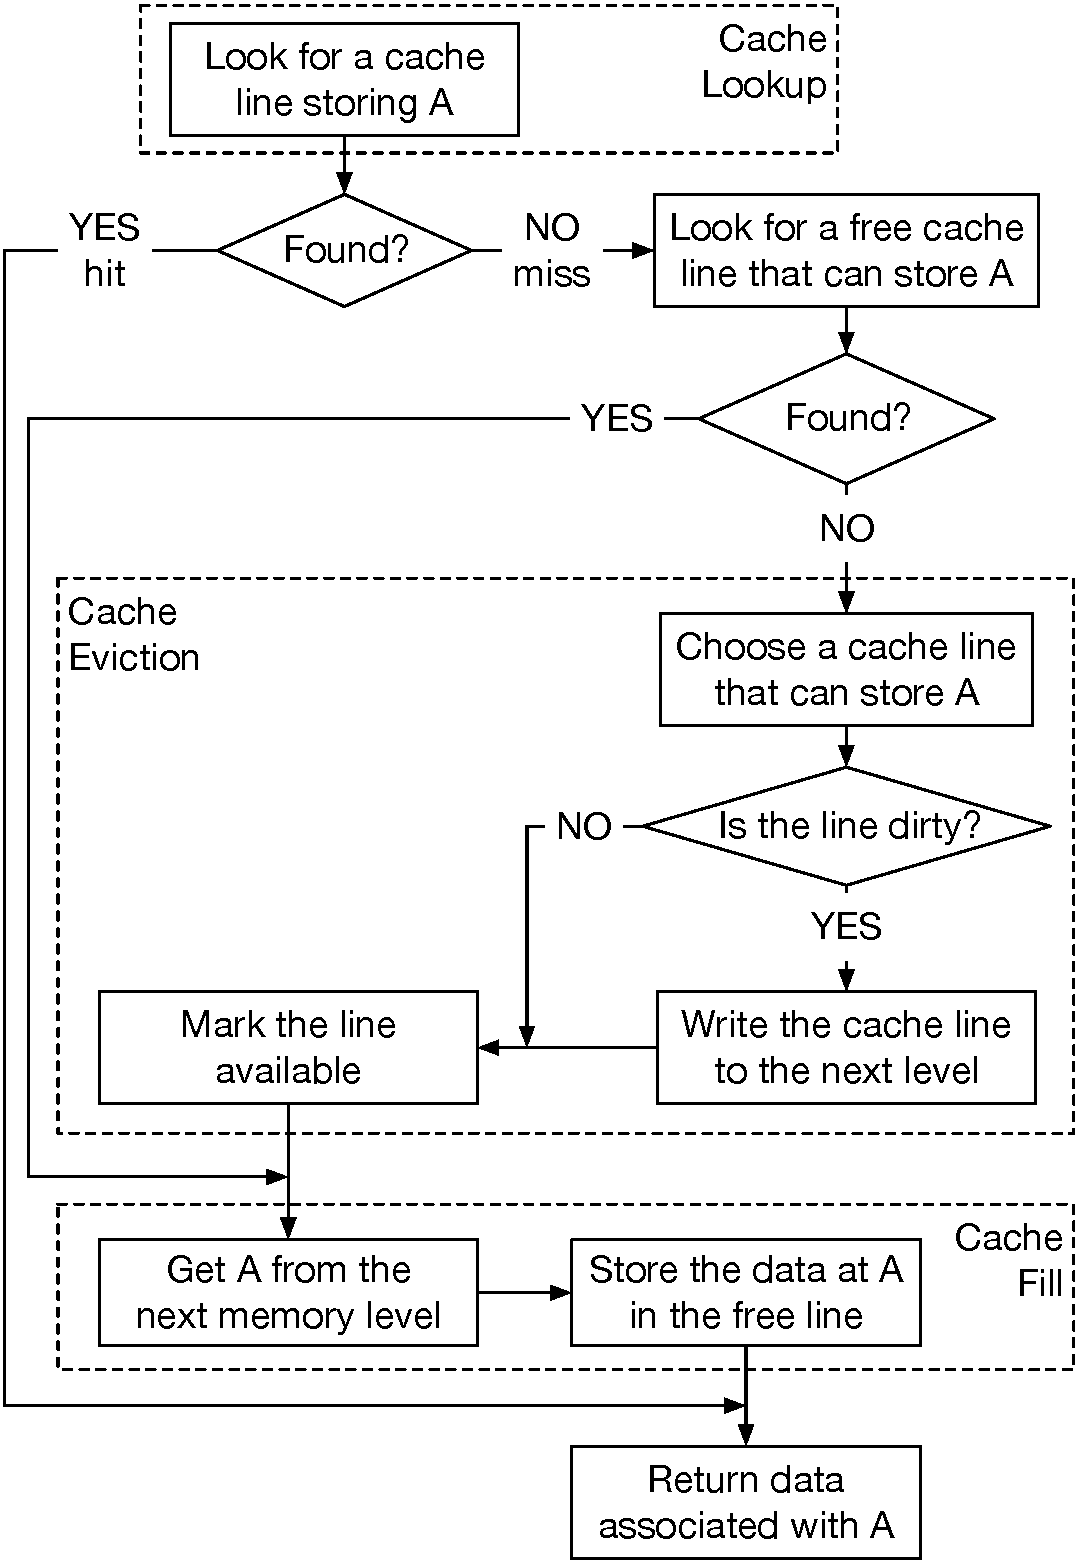
\includegraphics[width=80mm]{figures/cache_lookup.pdf}
  \caption{
    The steps taken by a cache memory to resolve an access to a memory address
    A. A normal memory access (to cacheable DRAM) always triggers a cache
    lookup. If the access misses the cache, a fill is required, and a
    write-back might be required.
  }
  \label{fig:cache_lookup}
\end{figure}

Unfortunately, caches create a dependency between the location of a memory
access and the time it takes to perform the access. A cache miss requires
at least one memory access to the next level cache, and might require a second
memory access if a write-back occurs. The related work presented in
\cite{banescu2011cache} shows that it is practical to use the timing
differences between hits and misses to learn the memory access patterns of a
target thread, as long as an attacker thread shares a cache with the target
thread. The target's memory access patterns, in turn, can reveal private
information, such as whether certain bits in an encryption key are set or not.

Table~\ref{fig:cache_timings} shows the key characteristics of the memory
hierarchy implemented by modern Intel CPUs. Each core has its own L1 and L2
cache (see Figure~\ref{fig:cpu_core}), while the L3 cache is in the CPU's
uncore (see Figure~\ref{fig:cpu_die}), and is shared by all the cores in the
package.

% Cache and Memory Subsystem: Optimization S 2.1.4
% Cache Hierarchy: Optimization S 2.2.5

\begin{table}[hbt]
  \centering
  \begin{tabular}{| l | r | r |}
  \hline
  \textbf{Memory} & \textbf{Size} & \textbf{Access Time}\\
  \hline
  Core Registers & 1~KB & no latency \\
  \hline
  L1 D-Cache & 32~KB & 4 cycles \\
  \hline
  L2 Cache & 256~KB & 10 cycles \\
  \hline
  L3 Cache & 8~MB & 40-75 cycles \\
  \hline
  DRAM & 16~GB & 60 ns \\
  \hline
  \end{tabular}
  \caption{
    Approximate sizes and access times for each level in the memory
    hierarchy of an Intel processor, from \cite{intel2010perfanalysis}. Memory
    sizes and access times differ by orders of magnitude across the different
    levels of the hierarchy. This table does not cover multi-processor systems.
  }
  \label{fig:cache_timings}
\end{table}

A cache timing attack that aims at the L2 cache would have to rely on the
system software to schedule a software thread on a logical processor in the
same core as the target software, whereas an attack on the L3 cache can be
performed using any logical processor on the same CPU. This implies that L3
cache attacks are feasible in an IaaS environment, whereas L2 cache attacks
become a possibility when running sensitive software on a user's desktop.

Our analysis of SGX concludes that it is vulnerable to cache timing attacks,
which can be used to obtain high-resolution memory access patterns for the
software running inside an SGX enclave.

\subsection{Interrupts}
\label{sec:interrupts}

Peripherals use \textit{interrupts} to signal the occurrence of an event that
must be handled by system software. For example, a keyboard issues interrupts
when a key is pressed or depressed. System software also relies on interrupts
to implement preemptive multi-threading. This section presents the details
needed to understand the concerns and tools that interrupts bring to the SGX
implementation.

% Advanced Programmable Interrupt Controller (APIC): SDM S 10
% Message Signalled Interrupts (MSI): SDM S 10.11

Peripherals use bus-specific protocols to signal interrupts. For example, PCIe
relies on \textit{Message Signaled Interrupts} (MSI), which are memory writes
issued to specially designed memory addresses. The bus-specific interrupt
signals are received by the \textit{I/O Advanced Programmable Interrupt
Controller} (IOAPIC) in the PCH, shown in Figure~\ref{fig:motherboard}.

% Local APIC ID: SDM S 10.4.6
% Extended xAPIC (x2APIC): SDM S 10.12

The IOAPIC routes interrupt signals to one or more \textit{Local Advanced
Programmable Interrupt Controllers} (LAPICs). As shown in
Figure~\ref{fig:cpu_die}, each logical CPU has a LAPIC that can receive
interrupt signals from the IOAPIC. The IOAPIC routing process assigns each
interrupt to an 8-bit \textit{interrupt vector}, used to identify the interrupt
sources, and a 32-bit \textit{APIC ID} used to identify the LAPIC that receives
the interrupt.

% Handling Interrupts: SDM S 10.8

Each LAPIC uses a 256-bit \textit{Interrupt Request Register} (IRR) to track
the un-serviced interrupts that it has received, based on the interrupt vector
number. When the corresponding logical processor is available, the LAPIC copies
the highest-priority un-serviced interrupt vector to the
\textit{In-Service Register} (ISR), and invokes the logical processor's
interrupt handling process.

% Issuing Interprocessor Interrupts: SDM S 10.6
% Interrupt Command Register (ICR): SDM S 10.6.1

At the architectural level, interrupt handling reuses many of the mechanisms in
fault handling (\S~\ref{sec:faults}). The interrupt vector number in the
LAPIC's ISR is used to locate an interrupt handler in the IDT, and the handler
is invoked, possibly after a privilege switch is performed. The interrupt
handler does the processing that the device requires, and then writes the
LAPIC's \textit{End Of Interrupt} (EOI) register to signal the fact that it has
completed handling the interrupt.

Interrupts are treated like faults, so interrupt handlers have full control
over the execution environment of the application being interrupted. This is
used to implement pre-emptive multi-threading, which relies on a clock device
that generates interrupts periodically, and on an interrupt handler that
performs context switches. While useful for multi-threading, this aspect of the
architecture also implies SGX design must include changes to the interrupt
handling process, in order to protect an enclave's execution state from an
interrupt handler that is invoked while an enclave's code is executing.

System software can cause an interrupt on any logical processor by writing the
target processor's APIC ID into the \textit{Interrupt Command Register} (ICR)
of the LAPIC associated with the logical processor that the software is runing
on. These interrupts, called \textit{Inter-Processor Interrupts} (IPI), are
needed to implement TLB shoot-downs (\S~\ref{sec:tlbs}). The IPI mechanism can
also be used to send SMI interrupts, which opens up an avenue for a malicious
kernel or hypervisor to mount a SMM mode (\S~\ref{sec:rings}) attack.

\subsection{The Boot Process}
\label{sec:booting}

When a computer is powered up, it undergoes a \textit{bootstrapping} process,
also called \textit{booting}, for simplicity. Although many steps in the boot
process depend on the motherboard and components in a computer, the process
does follow a high-level structure that is prescribed in the SDM. This section
provides the details needed to analyze SGX's security properties.
\cite{intel2010booting} provides a good reference on the entire booting
process.

% Initialization Overview: SDM S 9.1

Right after a computer is powered up, all the logical processors (LPs) on the
motherboard undergo \textit{hardware initialization}, which invalidates the
caches (\S~\ref{sec:caching}) and TLBs (\S~\ref{sec:tlbs}), performs a
\textit{Built-In Self Test} (BIST), and sets all the registers
(\S~\ref{sec:registers}) to pre-specified values.

% Multiple-Processor Initialization: SDM S 8.4
% BSP and AP Processors: SDM S 8.4.1
% MP Initialization Protocol Algorithms for MP Systems: SDM S 8.4.3
% An ivy bridge CPUID: family 06h, extended model 3, model 58, stepping 9

After hardware initialization, the LPs perform the Multi-Processor (MP)
initialization algorithm, which results in one LP being selected as the
\textit{bootstrap processor} (BSP), and all the other LPs being classified as
\textit{application processors} (APs).

According to the SDM, the details of the MP initialization algorithm for recent
CPUs depend on the motherboard and firmware. In principle, after completing
hardware initialization, all LPs attempt to issue a special no-op transaction
on the QPI bus. A single LP will suceed in issuing the no-op, thanks to
the QPI arbitration mechanism, and to the UBox (\S~\ref{sec:cache_coherence})
in each CPU package, which also serves as a ring arbiter. The arbitration
priority of each LP is based on its APIC ID APIC ID (\S~\ref{sec:interrupts}),
which is provided by the motherboard when the system powers up. The LP that
issues the no-op becomes the BSP. Upon failing to issue the no-op, the other
LPs become APs, and enter the \textit{wait-for-SIPI} state.

% Typical BSP Initialization Sequence: SDM S 8.4.4.1

The BSP sets its RIP register to point to the firmware reset code, which must
be present at 0xFFFFFFF0 (16 bytes below the 4 GB mark). This is accomplished
by having the initial SAD (\S~\ref{sec:cache_coherence}) and PCH
(\S~\ref{sec:motherboard}) configurations map the 4 KB below the 4 GB mark of
the memory address space (\S~\ref{sec:address_spaces}) to the SPI flash chip
that stores the motherboard's firmware.

\cite{intel2010booting} and \cite{coreboot2015manual} describe the
initialization steps performed by the firmware, from an implementor's
perspective. A few steps are interesting from the perspective of SGX and
caching attacks.

% Preventing Caching: SDM S 11.5.3

When the BSP starts executing firmware code, DRAM is not available. The
firmware places the BSP in \textit{Cache-as-RAM} (CAR) mode to be able to use a
call stack and other high-level constructs. Ater CAR is enabled, the memory
initialization code, which is typically Intel's \textit{Memory Reference Code}
(MRC), is loaded into the cache. When executed, the memory initialization code
discovers the DRAM chips connected to the motherboard and sets them up, and
enables and configures the memory controllers.

% Typical AP Initialization Sequence: SDM S 8.4.4.2


\subsection{CPU Microcode}
\label{sec:microcode}

% Outcome: evaluating the cost of architectural modifications

The Intel architecture features a large instruction set. Some instructions are
used infrequently, and some instructions are very complex, which makes it
impractical for an execution core to handle all the instructions in hardware.
Intel CPUs use a \textit{microcode} table to break down rare and complex
instructions into sequences of simpler instructions. Architectural extensions
that only require microcode changes are siginificantly cheaper to implement
and validate than extensions that require changes in the CPU's circuitry.

It follows that a good understanding of what can be done in microcode is
crucial to evaluating the cost of security features that rely on architecture
extensions. Furthermore, the limitations of microcode are sometimes the
reasoning behind seemingly arbitrary architecture design decisions.

The first sub-section below presents the relevant facts pertaining to microcode
in Intel's optimization reference \cite{intel2014optimization} and SDM. The
following subsections summarize information gleaned from Intel's patents and
other researchers' findings.


\subsubsection{The Role of Microcode}
\label{sec:microcode_role}

% Legacy Decode Pipeline (Instruction Decode): Optimization S 2.2.2.1
% Instruction Decode: Optimization S 2.3.2.4
% Front End Overview: Optimization S 2.4.2
% Understanding the Sources of the Micro-Op Queue: SDM S B.3.7.2

The frequently used instructions in the Intel architecture are handled by the
core's fast path, which consists of simple decoders (\S~\ref{sec:out_of_order})
that can emit at most 4 micro-ops per instruction. Infrequently used
instructions and instructions that require more than 4 micro-ops use a slower
decoding path that relies on a sequencer to read micro-ops from a
\textit{microcode store ROM} (MSROM).

The 4 micro-ops limitation can be used to guess intelligently whether an
architectural feature is implemented in microcode. For example, it is safe to
assume that \texttt{XSAVE} (\S~\ref{sec:registers}), which was takes over 200
micro-ops on recent CPUs \cite{fog2014microops}, is most likely performed in
microcode, whereas simple arithmetic and memory accesses are handled directly
by hardware.

% Assists: Optimization S B.3.5.2

The core's execution units handle common cases in fast paths implemented in
hardware. When an input cannot be handled by the fast paths, the execution
unit issues a \textit{microcode assist}, which points the microcode sequencer
to a routine in microcode that handles the edge cases. The most common cited
example in Intel's documentation is floating point instructions, which issue
assists to handle denormalized inputs.

The \texttt{REP MOVS} family of instructions, also known as \textit{string
instructions} because of their use in \texttt{strcpy}-like functions, operate
on variable-sized arrays. These instructions can handle small arrays in
hardware, and issue microcode assists for larger arrays.

% Microcode Update Facilities: SDM S 9.11
% Responsibilities of the BIOS: SDM 9.11.8.1

Modern Intel processors implement a microcode update facility. The SDM
describes microcode updates from the perspective of an OS kernel and
hypervisor. Each core can be updated independently, and the updates must be
reapplied on each boot cycle. A core can be updated multiple times, but each
update must have a bigger version than the core's current version. The latest
SDM at the time of this writing states that a microcode update is up to 16 KB
in size.

Processor engineers prefer to build new architectural features as microcode
extensions, because microcode can be iterated on much faster than hardware,
which reduces development cost \cite{intel2008genetic, intel2012clusters}. The
update facility further increases the appeal of microcode, as some classes of
bugs can be fixed after a CPU has been released.

Intel patents \cite{intel2013patent1, intel2013patent2} describing Software
Guard Extensions (SGX) disclose that SGX is entirely implemented in microcode,
except for the memory encryption engine. A description of SGX's implementation
could provide great insights into Intel's microcode, but, unfortunately, the
SDM chapters covering SGX do not include such a description. We therefore rely
on other public information sources about the role of microcode in the
security-sensitive areas covered by previous sections, namely memory
management~(\S~\ref{sec:paging}, \S~\ref{sec:tlbs}), the handling of hardware
exceptions~(\S~\ref{sec:faults}) and interrupts~(\S~\ref{sec:interrupts}), and
platform initialization~(\S~\ref{sec:booting}).

% Precise Event Based Sampling (PEBS): SDM S 18.7.1.1
% At-Retirement Counting: SDM S 18.13.6
% Performance Monitoring Events for the 4th Generation Intel Core Processors:
%     SDM S 19.3

The use of microcode assists can be measured using the
\textit{Precise Event Based Sampling} (PEBS) feature in recent Intel
processors. PEBS provides counters for the number of micro-ops coming from
MSROM, including complex instructions and assists, counters for the numbers of
assists associated with some micro-op classes (SSE and AVX stores and
transitions), and a counter for assists generated by all other micro-ops.

The PEBS feature itself is implemented using microcode assists (this is implied
in the SDM and confirmed by \cite{intel2014pebs}) when it needs to write the
execution context into a PEBS record. Given the wide range of features
monitored by PEBS counters, we assume that all execution units in the core can
issue microcode assists, which are performed at micro-op retirement (confirmed
by \cite{intel1997events}).

% Conditional SIMD Packed Loads and Stores: Optimization S 11.9

Intel's optimization manual describes one more interesting assist, from a
memory system perspective. SIMD masked loads (using \texttt{VMASKMOV}) read a
series of data elements from memory into a vector register. A mask register
decides whether elements are moved or ignored. If the memory address overlaps
an invalid page (e.g., the P flag is 0, \S~\ref{sec:paging}), a microcode
assist is issued, even if the mask indicates that no element from the invalid
page should be read. The microcode checks whether the elements in the invalid
page have the corresponding mask bits set, and either performs the load or
issues a page fault.

% IA32_MCG Extended Machine Check State MSRs: SDM S 15.3.2.6

The description of machine checks in the SDM mentions page assists and page
faults in the same context. We assume that the page assists are issued in some
cases when a TLB miss occurs (\S~\ref{sec:tlbs}) and the PMH has to walk the
page table. The following section develops this assumption and provides
supporting evidence from Intel's assigned patents and published patent
applications.


\subsubsection{Microcode Structure}
\label{sec:microcode_structure}

% Arch feature implementation strategy
%   US 8,447,962 - 11:39-43, 12:8-13

According to a 2013 Intel patent \cite{intel2013scattergather}, the avenues
considered for implementing new architectural features are a completely
microcode-based implementation, using existing micro-ops, a microcode
implementation with hardware support, which would use new micro-ops, and a
complete hardware implementation, using finite state machines (FSMs).

% Micro-ops table
%   US 7,451,121 - 1:23-25, 1:34-35, 2:64-65
%   US 8,099,587 - 3:1
% Microcode compression
%   US 7,451,121 - Abstract 1 and 10
%   US 8,099,587 - Abstract 1-3 and 7-10, 8:36-49, 11:10-17

The main component of the MSROM is a table of micro-ops \cite{intel2008genetic,
intel2012clusters}. According to an example in a 2012 Intel patent
\cite{intel2012clusters}, the table contains on the order of 20,000 micro-ops,
and a micro-op has about 70 bits. On embedded processors, like the Atom,
microcode may be partially compressed
\cite{intel2008genetic, intel2012clusters}.

% Event ROM
%   US 5,889,982 - 16:57-63, 16:66-17:3
% Microcode handles exceptions:
%   US 5,987,600 - 2:39-57, 4:13-27, 4:39-53, 4:65-5:6, 8:42-58, 10:54-60,
%                  11:18-42, 12:11-17, 12:54-58, 15:46-48, 15:59-62
%   US 5,889,982 - 11:40-42, 11:44-46
%   US 7,213,511 - 8:45-46, 8:49-51,
% Microcode handles traps:
%   US 5,987,600 - 15:16-18, 15:36-40
% Microcode handles interrupts:
%   US 5,987,600 - 16:2-5, 16:18-21
% Microcode handles events (exceptions and assists):
%   US 5,889,982 - 9:23-25, 9:34-42, 15:7-11, 15:27-55, 16:34-38, 16:57-17:3
%   US 5,625,788 - 1:10-12, 1:64-2:133:2-7, 6:31-38, 6:53-7:2, 8:27-47, 9:2-18,
%                  11:60-12:1, 12:4-8, 12:10-15, 12:19-12:22, 12:25-42,
%                  14:12-32

The MSROM also contains an event ROM, which is an array of pointers to event
handling code in the micro-ops table \cite{intel1999events}. Microcode events
are hardware exceptions, assists, and interrupts \cite{intel1997events,
intel1999exceptions, intel2007microstack}. The processor described in a 1999
patent \cite{intel1999events} has a 64-entry event table, where the first 16
entries point to hardware exception handlers and the other entries are used by
assists.

% Microcode implementation details:
%   US 5,987,600 - 5:39-49, 5:53-6:32, 5:35-39, 5:42-53, 11:53-60, 11:64-67,
%                  12:6-10, 12:41-45, 14:15-19
%   US 5,680,565 - 2:53-56
%   US 5,889,982 - 6:49-65, 7:8-12, 10:11-14, 13:16-20,
%   US 7,231,511 - 1:49-60, 2:1-8, 2:34-42, 3:2-5, 3:22-40, 5:26-67, 6:1-20
%   US 5,636,374 - 2:47-52, 2:63-3:10, 4:39-45

The execution units can issue an assist or signal a fault by associating an
event code with the result of a micro-op. When the micro-op is committed
(\S~\ref{sec:out_of_order}), the event code causes the out-of-order scheduler
to squash all the micro-ops that are in-flight in the ROB. The event code is
forwarded to the microcode sequencer, which reads the micro-ops in the
corresponding event handler \cite{intel1997events, intel1999exceptions}.

The hardware exception handling logic (\S~\ref{sec:faults}) and interrupt
handling logic (\S~\ref{sec:interrupts}) is implemented entirely in microcode
\cite{intel1999exceptions}. Therefore, changes to this logic are relatively
inexpensive to implement on Intel processors. This is rather fortunate, as the
Intel architecture's standard hardware exception handling process requires that
the fault handler is trusted by the code that encounters the exception
(\S~\ref{sec:faults}), and this assumption cannot be satisfied by a design
where the software executing inside a secure container must be isolated from
the system software managing the computer's resources.

% Microcode has microinstruction pointer stack
%   US 7,231,511 - Abstract 1-6, 2:44-45, 2:53-55, 3:9-16, 6:1-3, 12:2-9

The execution units in modern Intel processors support microcode procedures,
via dedicated microcode call and return micro-ops \cite{intel2007microstack}.
The micro-ops manage a hardware data structure that conceptually stores a stack
of microcode instruction pointers, and is integrated with out-of-order
execution and hardware exceptions, interrupts and assists.

% Microcode uses special loads / stores
%   US 5,636,374 - 2:31-36, 2:39-46, 6:10-19, 6:22-25, 6:53-57, 6:62-67,
%                  7:59-60, 8:13-24, 10:61-62, 10:65-12:64

Asides from special micro-ops, microcode also employs special load and store
instructions, which turn into special bus cycles, to issue commands to other
functional units \cite{intel1997microspace}. The memory addresses in the
special loads and stores encode commands and input parameters. For example,
stores to a certain range of addresses flush specific TLB sets.


\subsubsection{Microcode and Address Translation}
\label{sec:microcode_pmh}

% Microcode gets executed on CR3 write.
%   US 7,552,255 - 8:43-46

Address translation (\S~\ref{sec:paging}) is configured by CR3, which stores
the physical address of the top-level page table, and by various bits in CR0
and CR4, all of which are described in the SDM. Writes to these control
registers are implemented in microcode, which stores extra information in
microcode-visible registers \cite{intel2009pipeline}.

% DLB misses -> PMH, PMH uses a FSM.
%   US 13/730,563 - 0065, 0066, 0067
%   US 13/730,411 - 0064
%   US 5,564,111 - 1:26-29, 1:36-38, 3:7-21, 3:58-60, 5:36-41, 5:48-57,
%                  6:51-52, 6:55-7:7, 7:16-18, 7:23-24, 8:3-8, 8:39-40,
%                  9:66-10:4, 10:16-23
% PMH implementation (stuffed loads)
%   US 5,680,565 - 2:60-3:3, 3:25-28, 3:33-52, 3:56, 3:58-4:4, 11:17-21,
%                  11:45-48, 11:50-52, 12:30-34, 12:20-22, 12:40-43, 13:20-22,
%                  14:42-58, 15:54-57
%   US 5,636,374 - 5:59-64, 6:5-8
%   US 13/730,563 - 0072, 0073, 0074, Fig. 10

When a TLB miss (\S~\ref{sec:tlbs}) occurs, the memory execution unit forwards
the virtual address to the \textit{Page Miss Handler} (PMH), which performs the
page walk needed to obtain a physical address. In order to minimize the latency
of a page walk, the PMH is implemented as a finite-state machine (FSM)
\cite{hildesheim2014ptm, raikin2014tlb}. Furthermore, the PMH fetches the
page table entries from memory by issuing ``stuffed loads'', which are special
micro-ops that bypass the reorder buffer (ROB) and go straight to the memory
execution units (\S~\ref{sec:out_of_order}), thus avoiding the overhead
associated with out-of-order scheduling
\cite{intel1997pmh, intel1997microspace, hildesheim2014ptm}.

% Microcode handles memory exceptions (#PF):
%   US 5,987,600 - 14:26-49, 14:55-61, 14:66-15:3
%   US 5,680,565 - 11:29-37,
%   US 5,889,982 - 14:41-43, 15:47-51,
%   US 5,564,111 - 3:7-21, 3:58-60, 5:36-41, 5:48-57,
%                  6:51-52, 6:55-7:7, 7:16-18, 7:23-24, 8:3-8, 8:39-40,
%                  9:66-10:4, 10:16-23
% Microcode handles DTLB and PMH exceptions:
%   US 5,564,111 - Abstract 15-21, 1:46-59, 3:25-45, 7:47-53, 9:33-51,
%                  10:45-54, 10:57-63
% Microcode performs assisted PMH walk
%   US 5,680,565 - Abstract 1-2 and last 3 lines, 4:9-19, 4:22-28, 12:24-25,
%                  13:42-44, 13:48-54, 13:59-64, 14:12-21, 14:23-29, 14:61-66,
%                  15:1-12, 15:16-39

The FSM in the PMH handles the fast path of the entire address translation
process, which assumes no address translation fault (\S~\ref{sec:faults})
occurs
\cite{intel1996dtlb, intel1997pmh, intel1999exceptions, intel1999events}, and
no page table entry needs to be modified \cite{intel1997pmh}.

When the PMH FSM detects the conditions that trigger a Page Fault or a General
Protection Fault, it communicates a microcode event code, corresponding to the
detected fault condition, to the execution unit (\S~\ref{sec:out_of_order})
responsible for memory operations \cite{intel1996dtlb, intel1997pmh,
intel1999exceptions, intel1999events}. In turn, the execution unit triggers the
fault by associating the event code with the micro-op that caused the address
translation, as described in the previous section.

The PMH FSM does not set the accessed or dirty bits in page table entries. When
it detects that a page table entry must be modified, the FSM issues a microcode
event code for a page walk assist \cite{intel1997pmh}. The microcode handler
performs the page walk again, setting accessed and dirty bits on page table
entries when necessary \cite{intel1997pmh}.

The patents at the core of our descriptions above \cite{intel1996dtlb,
intel1997events, intel1997pmh, intel1999exceptions, intel1999events} were all
issued between 1996 and 1999, which raises the concern of obsolescence. As
Intel would not be able to file new patents for the same specifications, we
cannot present newer patents with the information above. Fortunately, we were
able to find newer patents that mention the techniques described above,
proving their relevance to newer CPU models.

% Microcode can prevent PMH writes
%   US 7,552,255 - 7:52-55

Two 2014 patents \cite{hildesheim2014ptm, raikin2014tlb} mention that the PMH
is executing a FSM which issues stuffing loads to obtain page table entries.
A 2009 patent \cite{intel2009pipeline} mentions that microcode is invoked after
a PMH walk, and that the microcode can prevent the translation result produced
by the PMH from being written to the TLB.

% VGATHER* / VSCATTER* - SDM instruction reference
% Microcode assists used for difficult cases in gather
%   US 8,688,962 - 5:26-30
% Scatter / gather implemented in microcode and hardware
%   US 8,447,962 - 11:28-30, 12:15-17, 12:20-23, 12:25-28

A 2013 patent \cite{intel2013scattergather} and a 2014 patent
\cite{intel2014gather} on scatter / gather instructions disclose that the newly
introduced instructions use a combination of hardware in the execution units
that perform memory operations, which include the PMH. The hardware issues
microcode assists for slow paths, such as gathering vector elements stored in
un-cacheable memory (\S~\ref{sec:memory_io}), and operations that cause Page
Faults.

% Microcode used when vAPIC memory checks fail
%   US 8,806,104 - 2:38-55, 3:12-17, 3:21-35, 3:39-43, 4:6-10, 4:29-42,
%                  4:55-57, 5:6-7, 5:10-17, 5:37-53, 5:58-60, 6:16-19,
%                  7:45-47, 8:30-36, 9:12-15

A 2014 patent on APIC (\S~\ref{sec:interrupts}) virtualization
\cite{intel2014vapic} describes a memory execution unit modification that
invokes a microcode assist for certain memory accesses, based on the contents
of some range registers. The patent also mentions that the range registers are
checked when the TLB miss occurs and the PMH is invoked, in order to decide
whether a fast hardware path can be used for APIC virtualization, or a
microcode assist must be issued.

The recent patents mentioned above allow us to conclude that the PMH in recent
processors still relies on an FSM and stuffed loads, and still uses microcode
assists to handle infrequent and complex operations. This assumption plays a
key role in estimating the implementation complexity of architectural
modifications targeting the processor's address translation mechanism.


\subsubsection{Microcode and Booting}
\label{sec:microcode_sec}

The SDM states that microcode performs the Built-In Self Test (BIST,
\S~\ref{sec:uefi_sec_details}), but does not provide any details on the
rest of the CPU's hardware initialization.

% Microcode initializes the CPU
%   US 8,806,104 - 4:36-41

% ACM is signed with a key in the CPU, verified by microcode
%   US 7,752,428 - 5:1-21
% EFI SEC and PEI core run in Cache-as-RAM mode, SEC loaded by microcode
%   US 7,752,428 - 5:22-28, 5:41-49, 5:56-5:67, 6:1-3, 6:9-13 6:44-6:58,
%                  7:11-45, Fig 4
%   US 8,296,528 - 7:39-50

% Microcode in ROM reads an ACM that measures firmware
%   US 8,429,418 - 2:14-28, 3:52-61, 4:2-8, Fig 1, Fig 2
% Microcode loads the ACM in Cache-as-RAM, authenticates using microcode crypto
%   US 8,429,418 - 4:13-20, 4:22-28
% Microcode runs at CPU reset and hashes an ACM in the firmware
%   US 8,321,931 - 6:47-52, 11:39-43, 11:45-47, 11:52-57, 12:6-11
%   US 8,301,907 - 4:8-10, 5:4-11, 5:16-17

In fact, the entire SEC implementation on Intel platforms is contained in the
processor microcode \cite{datta2010trustedboot, datta2013acm, intel2014vapic}.
This is a security measure, because  it is significantly more expensive for an
attacker to tamper with the MSROM circuitry (\S~\ref{sec:microcode_structure})
than it is to modify the contents of the flash memory chip that stores the
firmware (\S~\ref{sec:motherboard}).

The microcode that implements SEC performs MP initialization
(\S~\ref{sec:uefi_sec_details}), as suggested in the SDM. The microcode then
places the BSP into Cache-as-RAM (CAR) mode, looks up the PEI
\textit{Authenticated Code Module}~(ACM) in the Firmware Interface Table (FIT),
loads the PEI ACM into the cache, and verifies its signature
(\S~\ref{sec:uefi_sec_details}) \cite{datta2010trustedboot, intel2012patching,
intel2012uefihypervisor, intel2012ltsx, datta2013acm}. Given the structure of
ACM signatures, we can conclude that Intel's microcode contains implementations
of RSA decryption and of a variant of SHA hashing.

The PEI ACM is executed from the CPU's cache, after it is loaded by the
microcode \cite{datta2010trustedboot, intel2012patching, datta2013acm}. This
removes the possibility for an attacker with physical access to the SPI flash
chip to change the firmware's contents after the microcode computes its
cryptographic hash, but before it is executed.

% Microcode handles SIPI
%   US 8,301,907 - 4:31-33, Fig 2

On motherboards compatible with LaGrande Server Extensions (LT-SX, also known
as Intel TXT for servers), the firmware implementing PEI verifies that each CPU
connected to motherboard supports LT-SX, and powers off the CPU sockets that
don't have processors with LT-SX in them \cite{intel2012ltsx}. This prevents an
attacker from tampering with a TXT-protected VM by hot-plugging a CPU in a
running computer that is inside TXT mode. When a hot-plugged CPU passes
security tests, a hypervisor is notified that a new CPU is available. The
hypervisor updates its internal state, and sends the new CPU a SIPI. The new
CPU executes a SIPI handler, inside microcode, that configures the CPU's state
to match the state expected by the TXT hypervisor \cite{intel2012ltsx}. This
implies that the AP initialization described in \S~\ref{sec:uefi_sec_details}
is implemented in microcode.


\subsubsection{Microcode Updates}
\label{microcode:updates}

The SDM explains that the microcode on Intel CPUs can be updated, and describes
the process for applying an update. However, no detail about the contents of an
update is provided. Analyzing Intel's microcode updates seems like a promising
avenue towards discovering the microcode's structure. Unfortunately, the
updates have so far proven to be inscrutable \cite{chen2014microcode}.

% Microcode encryption
%   US 8,296,528 - 5:12-19

The microcode updates cannot be easily analyzed because they are encrypted,
hashed with a cryptographic hash function like SHA-256, and signed using RSA or
elliptic curve cryptography \cite{intel2012patching}. The update facility is
implemented entirely in microcode, including the decryption and signature
verification \cite{intel2012patching}.

\cite{hawkes2012microcode} independently used fault injection and timing
analysis to conclude that each recent Intel microcode update is signed with a
2048-bit RSA key and a (possibly non-standard) 256-bit hash algorithm, which
agrees with the findings above.

% Microcode sequesters cache ways
%   US 8,296,528 - 6:28-46, 7:9-34 7:48-51, 7:61-8:10, 8:12-57

The microcode update implementation places the core's cache into No-Evict Mode
(NEM, documented by the SDM) and copies the microcode update into the cache
before verifying its signature \cite{intel2012patching}. The update facility
also sets up an MTRR entry to protect the update's contents from modifications
via DMA transfers \cite{intel2012patching} as it is verified and applied.

While Intel publishes the most recent microcode updates for each of its CPU
models, the release notes associated with the updates are not publicly
available. This is unfortunate, as the release notes could be used to confirm
guesses that certain features are implemented in microcode.

However, some information can be inferred by reading through the Errata section
in Intel's Specification Updates
\cite{intel2010errata, intel2015errata, intel2015errata2}. The phrase ``it is
possible for BIOS\footnote{Basic Input/Output System (BIOS) is the predecessor
of UEFI-based firmware. Most Intel documentation, including the SDM, still uses
the term BIOS to refer to firmware.} to contain a workaround for this erratum''
generally means that a microcode update was issued. For example, Errata AH in
\cite{intel2010errata} implies that string instructions (\texttt{REP MOV}) are
implemented in microcode, which was confirmed by Intel
\cite{abraham2006repmov}.

% Microcode used for VMX instructions
%   US 8,806,104 - 2:61-66

Errata AH43 and AH91 in \cite{intel2010errata}, and AAK73 in
\cite{intel2015errata} imply that address translation (\S~\ref{sec:paging}) is
at least partially implemented in microcode. Errata AAK53, AAK63, and AAK70,
AAK178 in \cite{intel2015errata}, and BT138, BT210,  in \cite{intel2015errata2}
imply that VM entries and exits (\S~\ref{sec:faults}) are implemented in
microcode, which is confirmed by the APIC virtualization patent
\cite{intel2014vapic}.


\HeadingLevelB{SGX Security Properties}
\label{sec:sgx_security_analysis}

We have summarized SGX's programming model and the implementation details
that are publicly documented in Intel's official documentation and published
patents. We are now ready to bring this the information together in an analysis
of SGX's security properties. We start the analysis by restating SGX's
security guarantees, and spend the bulk of this section discussing how SGX
fares when pitted against the attacks described in
\S~\ref{sec:security_background}.


\HeadingLevelC{Overview}

Intel's Software Guard Extensions (SGX) is Intel's latest iteration of a
trusted hardware solution to the secure remote computation problem. The SGX
design is centered around the ability to create an isolated container whose
contents receives special hardware protections that are intended to translate
into privacy, integrity, and freshness guarantees.

% ISCA 2015 SGX: Slide 93

An enclave's initial contents is loaded by the system software on the computer,
and therefore cannot contain secrets in plain text. Once initialized, an
enclave is expected to participate in a software attestation process, where it
authenticates itself to a remote server. Upon successful authentication, the
remote server is expected to disclose some secrets to an enclave over a
secure communication channel. The SGX design attempts to guarantee that the
measurement presented during software attestation accurately represents the
contents loaded into the enclave.

SGX also offers a certificate-based identity system that can be used to migrate
secrets between enclaves that have certificates issued by the same authority.
The migration process involves securing the secrets via authenticated
encryption before handing them off to the untrusted system software, which
passes them to another enclave that can decrypt them.

The same mechanism used for secret migration can also be used to cache the
secrets obtained via software attestation in an untrusted storage medium
managed by system software. This caching can reduce the number of times that
the software attestation process needs to be performed in a distributed system.
In fact, SGX's software attestation process is implemented by enclaves with
special privileges that use the certificate-based identity system to securely
store the CPU's attestation key in untrusted memory.


\HeadingLevelC{Physical Attacks}
\label{sec:sgx_vs_physical_attacks}

We begin by discussing SGX's resilience to the physical attacks described in
\S~\ref{sec:physical_attacks}. Unfortunately, this section is set to disappoint
readers expecting definitive statements. The lack of publicly available details
around the hardware implementation aspects of SGX precludes any rigorous
analysis. However, we do know enough about SGX's implementation to point out a
few avenues for future exploration.

Due to insufficient documentation, one can only hope that the SGX security
model is not trivially circumvented by a port
attack~(\S~\ref{sec:physical_port_attacks}). We are particularly concerned
about the Generic Debug eXternal
Connection~(GDXC)~\cite{yuffe2011sandybridge, intel2011gdxc}, which collects
and filters the data transferred by the uncore's ring bus
(\S~\ref{sec:cache_coherence}), and reports it to an external debugger.

The SGX memory protection measures are implemented at the core level, in the
Page Miss Handler~(PMH,~\S~\ref{sec:tlbs}) (\S~\ref{sec:sgx_access_protection})
and at the chip die level, in the memory controller
(\S~\ref{sec:sgx_uncore_modifications}). Therefore, the code and data inside
enclaves is stored in plaintext in on-chip caches~(\S~\ref{sec:caching}), which
entails that the enclave contents travels without any cryptographic protection
on the uncore's ring bus (\S~\ref{sec:cache_coherence}).

Fortunately, a recent Intel patent~\cite{shanbhogue2015gdxcsgx} indicates that
Intel engineers are tackling at least some classes of attacks targeting
debugging ports.

The SDM and SGX papers discuss the most obvious class of bus tapping
attacks~(\S~\ref{sec:physical_bus_attacks}), which is the DRAM bus tapping
attack. SGX's threat model considers DRAM and the bus connecting it to the CPU
chip to be untrusted. Therefore, SGX's Memory Encryption
Engine~(MEE,~\S~\ref{sec:sgx_uncore_modifications}) provides privacy, integrity
and freshness guarantees to the Enclave Page Cache~(EPC,~\S~\ref{sec:sgx_epc})
data while it is stored in DRAM.

However, both the SGX papers and the ISCA 2015 tutorial on SGX admit that the
MEE does not protect the addresses of the DRAM locations accessed when cache
lines holding EPC data are evicted or loaded. This provides an opportunity for
a malicious computer owner to observe an enclave's memory access patterns by
combining a DRAM address line bus tap with carefully crafted system software
that creates artificial pressure on the last-level
cache~(LLC~,\S~\ref{sec:caching}) lines that hold the enclave's EPC pages.

On a brighter note, as mentioned in \S~\ref{sec:physical_bus_attacks}, we are
not aware of any successful DRAM address line bus tapping attack. Furthermore,
SGX is vulnerable to cache timing attacks that can be carried out completely in
software, so malicious computer owners do not need to bother setting up a
physical attack to obtain an enclave's memory access patterns.

While the SGX documentation addresses DRAM bus tapping attacks, it makes no
mention of the System Management bus~(SMBus,~\S~\ref{sec:intel_me}) that
connects the Intel Management Engine~(ME,~\S~\ref{sec:intel_me}) to various
components on the computer's motherboard.

In \S~\ref{sec:sgx_vs_device_attacks}, we will explain that the ME might play a
role in SGX's software attestation process. This makes us concerned about the
possibility of an attack that taps the SMBus to reach into the Intel ME. The
SMBus is much more accessible than the DRAM bus, as it has fewer wires that
operate at a significantly lower speed. Unfortunately, without more information
about the role that the Intel ME plays in a computer, we cannot move beyond
speculation on this topic.

The threat model stated by the SGX design excludes physical attacks targeting
the CPU chip~(\S~\ref{sec:physical_chip_attacks}). Fortunately, Intel's patents
disclose an array of countermeasures aimed at increasing the cost of chip
attacks.

For example, the original SGX patents~\cite{intel2013patent1, intel2013patent2}
disclose that the Fused Seal Key and the Provisioning Key, which are stored in
e-fuses (\S~\ref{sec:sgx_quoting_enclave}), are encrypted with a \textit{global
wrapping logic key}~(GWK). The GWK is a 128-bit AES key that is hard-coded in
the processor's circuitry, and serves to increase the cost of extracting the
keys from an SGX-enabled processor.

As explained in \S~\ref{sec:physical_chip_attacks}, e-fuses have a large
feature size, which makes them relatively easy to ``read'' using a
high-resolution microscope. In comparison, the circuitry on the latest Intel
processors has a significantly smaller feature size, and is more difficult to
reverse engineer. Unfortunately, the GWK is shared among all the chip dies
created from the same mask, so it has all the drawbacks of global secrets
explained in \S~\ref{sec:physical_chip_attacks}.

Newer Intel patents~\cite{gotze2014provisioning, gotze2014provisioning2}
describe SGX-enabled processors that employ a \textit{Physical Unclonable
Function}~(PUF), e.g., \cite{suh2007puf}, \cite{maes2009puf}, which generates a
symmetric key that is used during the provisioning process.

Specifically, at an early provisioning stage, the PUF key is encrypted with the
GWK and transmitted to the key generation server. At a later stage, the key
generation server encrypts the key material that will be burned into the
processor chip's e-fuses with the PUF key, and transmits the encrypted material
to the chip. The PUF key increases the cost of obtaining a chip's fuse key
material, as an attacker must compromise both provisioning stages in order to
be able to decrypt the fuse key material.

As mentioned in previous sections, patents reveal design possibilities
considered by the SGX engineers. However, due to the length of timelines involved
in patent applications, patents necessarily describe earlier versions of the
SGX implementation plans, which might not match the shipping implementation. We
expect this might be the case with the PUF provisioning patents, as it makes
little sense to include a PUF in a chip die and rely on e-fuses and a GWK to
store SGX's root keys. Deriving the root keys from the PUF would be more
resilient to chip imaging attacks.

SGX's threat model excludes power analysis
attacks~(\S~\ref{sec:power_analysis_attacks}) and other side-channel attacks.
This is understandable, as power attacks cannot be addressed at the
architectural level. Defending against power attacks requires expensive
countermeasures at the lowest levels of hardware implementation, which can only
be designed by engineers who have deep expertise in both system security and
Intel's manufacturing process. It follows that defending against power analysis
attacks has a very high cost-to-benefit ratio.


\HeadingLevelC{Privileged Software Attacks}
\label{sec:sgx_vs_privileged_sw_attacks}

The SGX threat model considers system software to be untrusted. This is a
prerequisite for SGX to qualify as a solution to the secure remote computation
problem encountered by software developers who wish to take advantage of
Infrastructure-as-a-Service (IaaS) cloud computing.

SGX's approach is also an acknowledgement of the realities of today's software
landscape, where the system software that runs at high privilege
levels~(\S~\ref{sec:rings}) is so complex that security researchers constantly
find vulnerabilities in it (\S~\ref{sec:system_software_attacks}).

The SGX design prevents malicious software from directly reading or from
modifying the EPC pages that store an enclave's code and data. This security
property relies on two pillars in the SGX design.

First, the SGX implementation~(\S~\ref{sec:sgx_implementation_overview}) runs
in the processor's microcode~(\S~\ref{sec:microcode}), which is effectively a
higher privilege level that system software does not have access to.
Along the same lines, SGX's security
checks~(\S~\ref{sec:sgx_access_protection}) are the last step performed by the
PMH, so they cannot be bypassed by any other architectural feature.

This implementation detail is only briefly mentioned in SGX's official
documentation, but has a large impact on security. For context, Intel's Trusted
Execution Technology~(TXT,~\cite{grawrock2009txt}), which is the predecessor of
SGX, relied on Intel's Virtual Machine Extensions (VMX) for isolation. The
approach was unsound, because software running in System Management
Mode~(SMM,~\S~\ref{sec:rings}) could bypass the restrictions used by VMX to
provide isolation.

The security properties of SGX's memory protection mechanisms are discussed
in detail in \S~\ref{sec:sgx_vs_memory_mapping_attacks}.

Second, SGX's microcode is always involved when a CPU transitions between
enclave code and non-enclave code~(\S~\ref{sec:sgx_threads}), and therefore
regulates all interactions between system software and an enclave's
environment.

On enclave entry~(\S~\ref{sec:sgx_eenter}), the SGX implementation sets up the
registers~(\S~\ref{sec:resources}) that make up the execution
state~(\S~\ref{sec:registers}) of the logical
processor~(LP~\S~\ref{sec:cpu_core}), so a malicious OS or hypervisor cannot
induce faults in the enclave's software by tampering with its execution
environment.

When an LP transitions away from an enclave's code due to a
hardware exception~(\S~\ref{sec:faults}), the SGX implementation stashes the
LP's execution state into a State Save Area~(SSA,~\S~\ref{sec:sgx_ssa}) area
inside the enclave and scrubs it, so the system software's exception handler
cannot access any enclave secrets that may be stored in the execution state.

The protections described above apply to the all the levels of privileged
software. SGX's transitions between an enclave's code and non-enclave code
place SMM software on the same footing as the system software at lower
privilege levels. System Management Interrupts~(SMI,~\S~\ref{sec:interrupts},
\S~\ref{sec:system_software_attacks}), which cause the processor to execute
SMM code, are handled using the same Asynchronous Enclave
Exit~(AEX,~\S~\ref{sec:sgx_aex}) process as all other hardware exceptions.

Unfortunately, the following sections will reveal that while SGX offers rather
thorough against straightforward attacks on enclaves, its guarantees are almost
non-existent when it comes to more sophisticated attacks, such as side-channel
attacks. This section concludes by describing what might be the most egregious
side-channel vulnerability in SGX.

Most modern Intel processors feature hyper-threading. On these CPUs, the
execution units~(\S~\ref{sec:out_of_order}) and caches~(\S~\ref{sec:caching})
on a core~(\S~\ref{sec:cpu_core}) are shared by two LPs, each of which has its
own execution state. SGX does not prevent hyper-threading, so malicious system
software can schedule a thread executing the code of a victim enclave on an
LP that shares the core with an LP executing a snooping thread. This snooping
thread can use the processor's high-resolution performance counter
\cite{petters1999making}, in conjunction with microarchitectural knowledge of
the CPU's execution units and out-of-order scheduler, to learn the instructions
executed by the victim enclave, as well as its memory access patterns.

This vulnerability can be fixed using two approaches. The straightforward
solution is to require cloud computing providers to disable hyper-threading
when offering SGX. The SGX enclave measurement would have to be extended to
include the computer's hyper-threading configuration, so the remote parties in
the software attestation process can be assured that their enclaves are hosted
by a secure environment.

A more complex approach to fixing the hyper-threading vulnerability would
entail having the SGX implementation guarantee that when an LP is executing an
enclave's code, the other LP sharing its core is either inactive, or is
executing the same enclave's code. While this approach is possible, its design
would likely be quite cumbersome.


\HeadingLevelC{Memory Mapping Attacks}
\label{sec:sgx_vs_memory_mapping_attacks}

\S~\ref{sec:sgx_threads} explained that the code running inside an enclave uses
the same address translation process~(\S~\ref{sec:paging}) and page tables as
its host application. While this design approach makes it easy to retrofit SGX
support into existing codebases, it also enables the address translation
attacks described in \S~\ref{sec:address_translation_attacks}.

The SGX design protects the code inside enclaves against the active attacks
described in \S~\ref{sec:address_translation_attacks}. These protections have
been extensively discussed in prior sections, so we limit ourselves to
pointing out SGX's answer to each active attack. We also explain the lack of
protections against passive attacks, which can be used to learn an enclave's
memory access pattern at 4KB page granularity.

SGX uses the Enclave Page Cache Map~(EPCM,~\S~\ref{sec:sgx_epcm}) to store each
EPC page's position in its enclave's virtual address space. The EPCM is
consulted by SGX's extensions to the Page Miss
Handler~(PMH,~\S~\ref{sec:sgx_access_concepts}), which prevent straightforward
active address translation attacks~(\S~\ref{sec:memory_mapping_attacks}) by
rejecting undesirable address translations before they reach the
TLB~(\S~\ref{sec:tlbs}).

SGX allows system software to evict~(\S~\ref{sec:sgx_epc_eviction}) EPC pages
into untrusted DRAM, so that the EPC can be over-subscribed. The contents of
the evicted pages and the associated EPCM metadata are protected by
cryptographic primitives that offer privacy, integrity and freshness
guarantees. This protects against the active attacks using page swapping
described in \S~\ref{sec:page_swapping_attacks}.

When system software wishes to evict EPC pages, it must follow the process
described in \S~\ref{sec:sgx_eblock}, which guarantees to the SGX
implementation that all the LPs have invalidated any TLB entry associated with
pages that will be evicted. This defeats the active attacks based on stale TLB
entries described in \S~\ref{sec:tlb_mapping_attacks}.

\S~\ref{sec:sgx_access_correctness} outlines a correctness proof for all the
protection measures described above.

Unfortunately, SGX does not protect against passive address translation
attacks~(\S~\ref{sec:fault_tracking_attacks}), which can be used to learn an
enclave's memory access pattern at page granularity. While this appears
benign, recent work \cite{xu2015pagefaults} demonstrates the use of these
passive attacks in a few practical settings, which are immediately concerning
for image processing applications.

The rest of this section describes the theory behind planning a passive attack
against an SGX enclave. The reader is directed to \cite{xu2015pagefaults} for
a fully working system.

Passive address translation attacks rely on the fact that memory accesses
issued by SGX enclaves go through the Intel architecture's address translation
process~(\S~\ref{sec:paging}), including delivering page
faults~(\S~\ref{sec:faults}) and setting the accessed (A) and dirty (D)
attributes~(\S~\ref{sec:page_table_attributes}) on page table entries.

A malicious OS kernel or hypervisor can obtain the page-level trace of an
application executing inside an enclave by setting the present (P) attribute to
0 on all the enclave's pages before starting enclave execution. While an
enclave executes, the malicious system software maintains exactly one
instruction page and one data page present in the enclave's address space.

When a page fault is generated, CR2 contains the virtual address of a page
accessed by enclave, and the error code indicates whether the memory access was
a read or a write (bit 1) and whether the memory access is a data access or
an instruction fetch access (bit 4). On a data access, the kernel tracing the
enclave code's memory access pattern would set the P flag of the desired page
to 1, and set the P flag of the previously accessed data page to 0. Instruction
accesses can be handled in a similar manner.

For a slightly more detailed trace, the kernel can set a desired page's
writable (W) attribute to 0 if the page fault's error code indicates a read
access, and only set it to 1 for write accesses. Also, applications that use a
page as both code and data (self-modifying code and just-in-time compiling VMs)
can be handled by setting a page's disable execution (XD) flag to 0 for a data
access, and by carefully accounting for the case where the last accessed data
page is the same as the last accessed code page.

Leaving an enclave via an Asynchronous Enclave Exit~(AEX,~\S~\ref{sec:sgx_aex})
and re-entering the enclave via \texttt{ERESUME}~(\S~\ref{sec:sgx_eresume})
causes the CPU to flush TLB entries that contain enclave addresses, so a
tracing kernel would not need to worry about flushing the TLB. The tracing
kernel does not need to flush the caches either, because the CPU needs to
perform address translation even for cached data.

A straightforward way to reduce this attack's power is to increase the page
size, so the trace contains less information. However, the attack cannot be
completely prevented without removing the kernel's ability to oversubscribe the
EPC, which is a major benefit of paging.


\HeadingLevelC{Software Attacks on Peripherals}
\label{sec:sgx_vs_device_attacks}

Since the SGX design does not trust the system software, it must be prepared to
withstand the attacks described in \S~\ref{sec:device_attacks}, which can be
carried out by the system software thanks to its ability to control peripheral
devices on the computer's motherboard~(\S~\ref{sec:motherboard}). This section
summarizes the security properties of SGX when faced with these attacks, based
on publicly available information.

When SGX is enabled on an LP, it configures the memory
controller~(MC,~\S~\ref{sec:cache_coherence}) integrated on the CPU chip die to
reject any DMA transfer that falls within the Processor Reserved
Memory~(PRM,~\S~\ref{sec:sgx_prm}) range. The PRM includes the EPC, so the
enclaves' contents is protected from the PCI Express attacks described in
\S~\ref{sec:pcie_attacks}. This protection guarantee relies on the fact that
the MC is integrated on the processor's chip die, so the MC configuration
commands issued by SGX's microcode
implementation~(\S~\ref{sec:sgx_microcode_modifications}) are transmitted over
a communication path that never leaves the CPU die, and therefore can be
trusted.

SGX regards DRAM as an untrusted storage medium, and uses cryptographic
primitives implemented in the MEE to guarantee the privacy, integrity and
freshness of the EPC contents that is stored into DRAM. This protects against
software attacks on DRAM's integrity, like the rowhammer attack described in
\S~\ref{sec:rowhammer_attack}.

% Interaction with Performance Monitoring: SDM S 43.6

The SDM describes an array of measures that SGX takes to disable processor
features intended for debugging when a LP starts executing an enclave's code.
For example, enclave entry~(\S~\ref{sec:sgx_eenter}) disables Precise Event
Based Sampling (PEBS) for the LP, as well as any hardware breakpoints placed
inside the enclave's virtual address range~(ELRANGE,~\S~\ref{sec:sgx_elrange}).
This addresses some of the attacks described in \S~\ref{sec:perfmon_attacks},
which take advantage of performance monitoring features to get information that
typically requires access to hardware probes.

% ISCA 2015 SGX Slide 115:
%   "Software Side-Channel Adversary"

At the same time, the SDM does not mention anything about uncore PEBS counters,
which can be used to learn about an enclave's LLC activity. Furthermore, the
ISCA 2015 tutorial slides mention that \textbf{SGX does not protect against
software side-channel attacks} that rely on performance counters.

This limitation in SGX's threat model leaves security-conscious enclave authors
in a rather terrible situation. These authors know that SGX does not protect
their enclaves against a class of software attacks. At the same time, they
cannot even contemplate attempting to defeat these attacks on their own, due to
lack of information. Specifically, the documentation that is publicly available
from Intel does not provide enough information to model the information leakage
due to performance counters.

For example, Intel does not document the mapping implemented in
CBoxes~(\S~\ref{sec:cache_coherence}) between physical DRAM addresses and the
LLC slices used to cache the addresses. This mapping impacts several uncore
performance counters, and the impact is strong enough to allow security
researches to reverse-engineer the mapping \cite{inci2015rsachannel,
maurice2015intelhash, yarom2015intelhash}. Therefore, it is safe to assume that
a malicious computer owner who knows the CBox mapping can use the uncore
performance counters to learn about an enclave's memory access patterns.

The SGX papers mention that SGX's threat model includes attacks that overwrite
the flash memory chip that stores the computer's firmware, which result in
malicious code running in SMM.  However, all the official SGX documentation is
silent about the implications of an attack that compromises the firmware
executed by the Intel ME.

\S~\ref{sec:firmware_attacks} states that the ME's firmware is stored in the
same flash memory as the boot firmware, and enumerates some of ME's special
privileges that enable it to help system administrators remotely diagnose and
fix hardware and software issues. Given that the SGX design is concerned about
the possibility of malicious computer firmware, it is reasonable to be
concerned about malicious ME firmware.

\S~\ref{sec:firmware_attacks} argues that an attacker who compromises the ME
can carry out actions that are usually classified as physical attacks.
Fortunately, the most scary attack vector afforded by an ME takeover appears to
be direct DRAM access, and SGX already assumes that the DRAM is untrusted.
Therefore, an ME compromise would be equivalent to the DRAM attacks analyzed in
\S~\ref{sec:sgx_vs_physical_attacks}.


\HeadingLevelC{Cache Timing Attacks}
\label{sec:sgx_vs_cache_timing_attacks}

The SGX threat model excludes the cache timing attacks described in
\S~\ref{sec:cache_timing}. The SGX documentation bundles these attacks together
with other side-channel attacks and summarily dismisses them as complex physical
attacks. However, cache timing attacks can be mounted entirely by unprivileged
software running at ring 3. This section describes the implications of SGX's
environment and threat model on cache timing attacks.

The main difference between SGX and a standard architecture is that SGX's
threat model considers the system software to be untrusted. As explained
earlier, this accurately captures the situation in remote computation
scenarios, such as cloud computing. SGX's threat model implies that the system
software can be carrying out a cache timing attack on the software inside an
enclave.

A malicious system software translates into significantly more powerful cache
timing attacks, compared to those described in \S~\ref{sec:cache_timing}. The
system software is in charge of scheduling threads on LPs, and also in charge
of setting up the page tables used by address
translation~(\S~\ref{sec:paging}), which control cache
placement~(\S~\ref{sec:tlbs}).

For example, the malicious kernel set out to trace an enclave's memory access
patterns described in \S~\ref{sec:sgx_vs_memory_mapping_attacks} can improve
the accuracy of a cache timing attack by using page
coloring~\cite{kessler1992coloring} principles to
partition~\cite{lin2008coloring} the cache targeted by the attack. In a
nutshell, the kernel divides the cache's sets~(\S~\ref{sec:cache_org}) into
two regions, as shown in Figure~\ref{fig:cache_partitions}.

\begin{figure}[hbt]
  \centering
  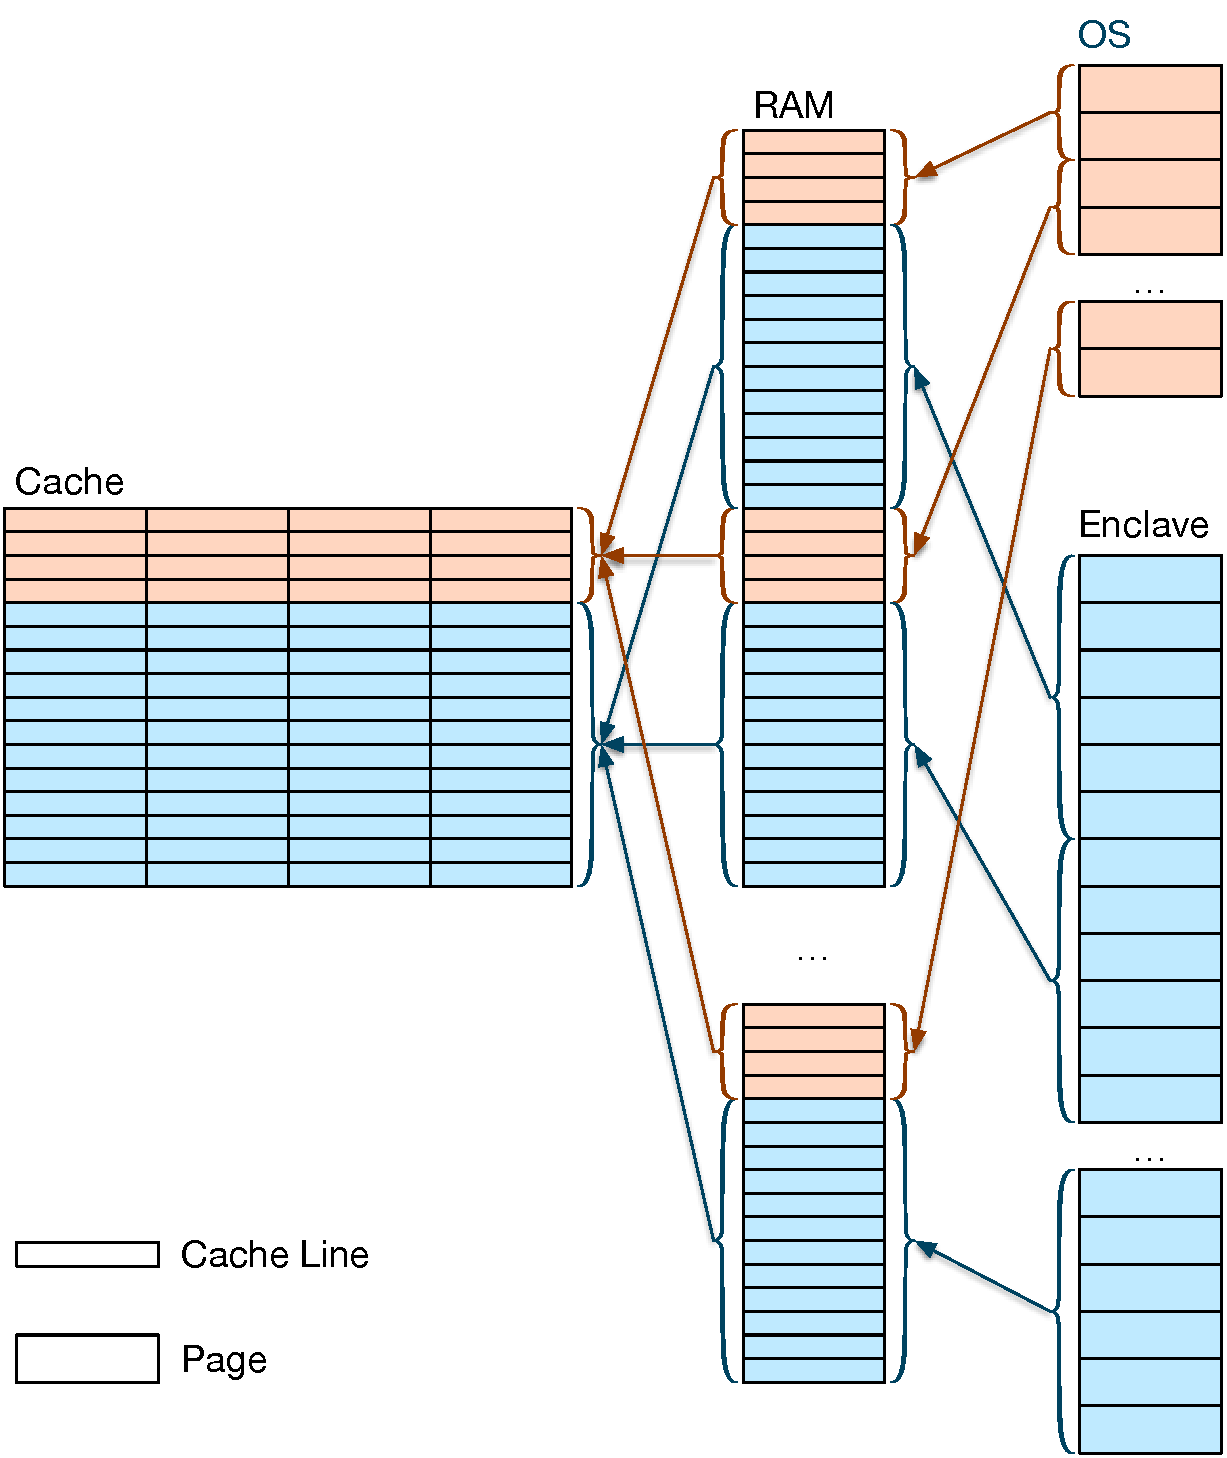
\includegraphics[width=85mm]{figures/cache_partitions.pdf}
  \caption{
    A malicious OS can partition a cache between the software running inside an
    enclave and its own malicious code. Both the OS and the enclave software
    have cache sets dedicated to them. When allocating DRAM to itself and to
    the enclave software, the malicious OS is careful to only use DRAM regions
    that map to the appropriate cache sets. On a system with an Intel CPU, the
    the OS can partition the L2 cache by manipulating the page tables in a way
    that is completely oblivious to the enclave's software.
  }
  \label{fig:cache_partitions}
\end{figure}

The system software stores all the victim enclave's code and data in DRAM
addresses that map to the cache sets in one of the regions, and stores its own
code and data in DRAM addresses that map to the other region's cache sets.  The
snooping thread's code is assumed to be a part of the OS. For example, in a
typical 256~KB (per-core) L2 cache organized as 512 8-way sets of 64-byte
lines, the tracing kernel could allocate lines 0-63 for the enclave's code
page, lines 64-127 for the enclave's data page, and use lines 128-511 for its
own pages.

To the best of our knowledge, there is no minor modification to SGX that would
provably defend against cache timing attacks. However, the SGX design could
take a few steps to increase the cost of cache timing attacks. For example,
SGX's enclave entry implementation could flush the core's private caches, which
would prevent cache timing attacks from targeting them. This measure would
defeat the cache timing attacks described below, and would only be vulnerable
to more sophisticated attacks that target the shared LLC, such as
\cite{yarom2013llctiming, liu2015llctiming}. The description above assumes that
multi-threading has been disabled, for the reasons explained in
\S~\ref{sec:sgx_vs_privileged_sw_attacks}.

Barring the additional protection measures described above, a tracing kernel
can extend the attack described in \S~\ref{sec:sgx_vs_memory_mapping_attacks}
with the steps outlined below to take advantage of cache timing and narrow down the
addresses in an application's memory access trace to cache line granularity.

Right before entering an enclave via \texttt{EENTER} or \texttt{ERESUME}, the
kernel would issue \texttt{CLFLUSH} instructions to flush the enclave's code
page and data page from the cache. The enclave could have accessed a single
code page and a single data page, so flushing the cache should be reasonably
efficient. The tracing kernel then uses 16 bogus pages (8 for the enclave's
code page, and 8 for the enclave's data page) to load all the 8 ways in the 128
cache sets allocated by enclave pages. After an AEX gives control back to the
tracing kernel, it can read the 16 bogus pages, and exploit the time difference
between an L2 cache hit and a miss to see which cache lines were evicted and
replaced by the enclave's memory accesses.

% PRMRR documented in HASP papers and both SGX manuals, completely removed from
% SDM. It still exists in Coreboot. Couldn't find other Skywell code.

An extreme approach that can provably defeat cache timing attacks is disabling
caching for the PRM range, which contains the EPC. The SDM is almost completely
silent about the PRM, but the SGX manuals that it is based on state that
the allowable caching behaviors~(\S~\ref{sec:cacheability_config}) for the EPC
are uncacheable (UC) and write-back (WB). This could become useful if the SGX
implementation would make sure that the PRM's caching behavior cannot be
changed while SGX is enabled, and if the selected behavior would be captured by
the enclave's measurement~(\S~\ref{sec:sgx_measurement}).

\section{Related Work}
\label{sec:related}

This section describes the broader picture of trusted hardware projects that
SGX belongs to. Table~\ref{fig:secure_processors} summarizes the security
properties of SGX and the other trusted hardware presented here.

\begin{table*}
  \centering
  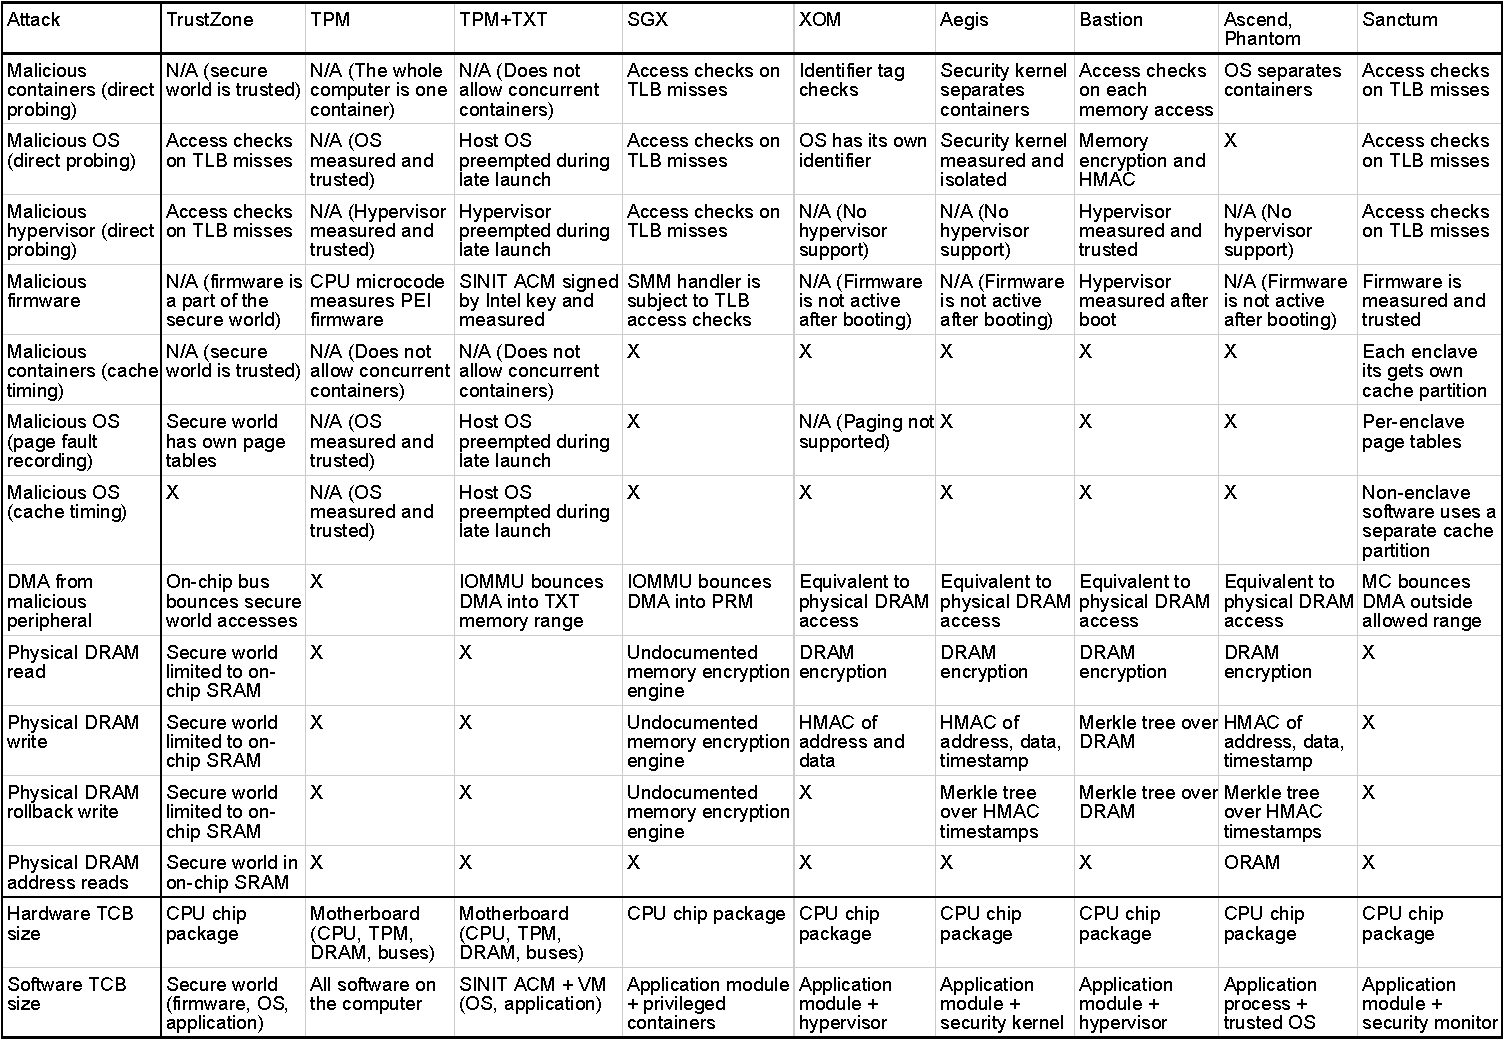
\includegraphics[angle=90,width=170mm]{figures/secure_processors_table.pdf}
  \caption{
    Security features overview for the trusted hardware projects related to
    Intel's SGX
  }
  \label{fig:secure_processors}
\end{table*}


\subsection{The IBM 4765 Secure Coprocessor}

Secure coprocessors~\cite{yee1994coprocessors} encapsulate an entire computer
system, including a CPU, a cryptographic accelerator, caches, DRAM, and an I/O
controller within a tamper-resistant environment. The enclosure includes
hardware that deters attacks, such as a Faraday cage, as well as an array of
sensors that can detect tampering attempts. The secure coprocessor destroys the
secrets that it stores when an attack is detected. This approach has good
security properties against physical attacks, but tamper-resistant enclosures
are very expensive~\cite{anderson2001security}, relatively to the cost of a
computer system.

The IBM 4758~\cite{smith1999ibm4758}, and its most current-day successor, the
IBM 4765~\cite{nist2015ibm4765} (shown in Figure~\ref{fig:ibm_4765}) are
representative examples of secure coprocessors. The 4758 was certified to
withstand physical attacks to FIPS 140-1 Level 4~\cite{smith1999validating},
and the 4765 meets the rigors of FIPS 140-2 Level 4~\cite{nist2011fipscert}.

\begin{figure}[hbt]
  \centering
  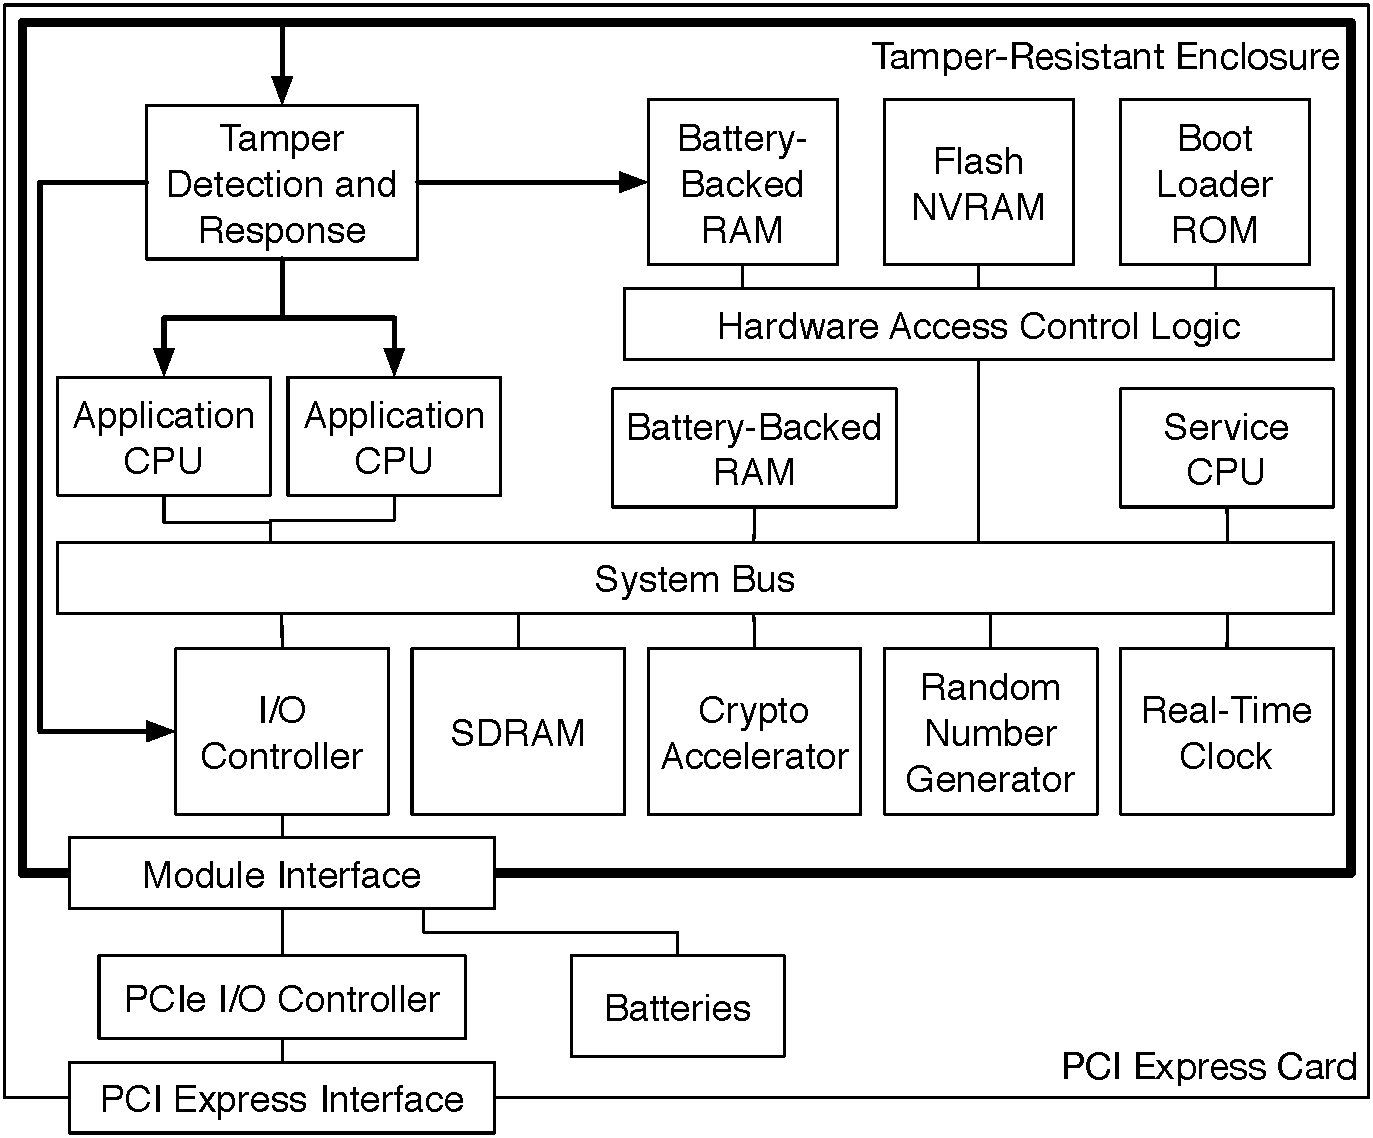
\includegraphics[width=85mm]{figures/ibm_4765.pdf}
  \caption{
    The IBM 4765 secure coprocessor consists of an entire computer system
    placed inside an enclosure that can deter and detect physical attacks.
    The application and the system use separate processors. Sensitive memory
    can only be accessed by the system code, thanks to access control checks
    implemented in the system bus' hardware. Dedicated hardware is used to clear
    the platform's secrets and shut down the system when a physical attack is
    detected.
  }
  \label{fig:ibm_4765}
\end{figure}

The 4765 relies heavily on physical isolation for its security properties. Its
system software is protected from attacks by the application software by
virtue of using a dedicated service processor that is completely separate from
the application processor. Special-purpose bus logic prevents the application
processor from accessing privileged resources, such as the battery-backed
memory that stores the system software's secrets.

The 4765 implements software attestation. The coprocessor's attestation key is
stored in battery-backed memory that is only accessible by the service
processor. Upon reset, the service processor executes a first-stage bootloader
stored in ROM, which measures and loads the system software. In turn, the
system software measures the application code stored in NVRAM and loads it into
the DRAM chip accessible to the application processor. The system software
provides attestation services to the application loaded inside the coprocessor.

\subsection{ARM TrustZone}

ARM's TrustZone~\cite{alves2004trustzone} is a collection of hardware modules
that can be used to conceptually partition a system's resources between a
\textit{secure world}, which hosts a secure container, and a \textit{normal
world}, which runs an untrusted software stack. The TrustZone
documentation~\cite{arm2009trustzone} describes semiconductor intellectual
property cores (IP blocks) and ways in which they can be combined to achieve
certain security properties, reflecting the fact that ARM is an IP core
provider, not a chip manufacturer. Therefore, the mere presence of TrustZone IP
blocks in a system is not sufficient to determine whether the system is secure
under a specific threat model. Figure~\ref{fig:trustzone} illustrates a design
for a smartphone \textit{System-on-Chip} (SoC) design that uses TrustZone IP
blocks.

\begin{figure}[hbt]
  \centering
  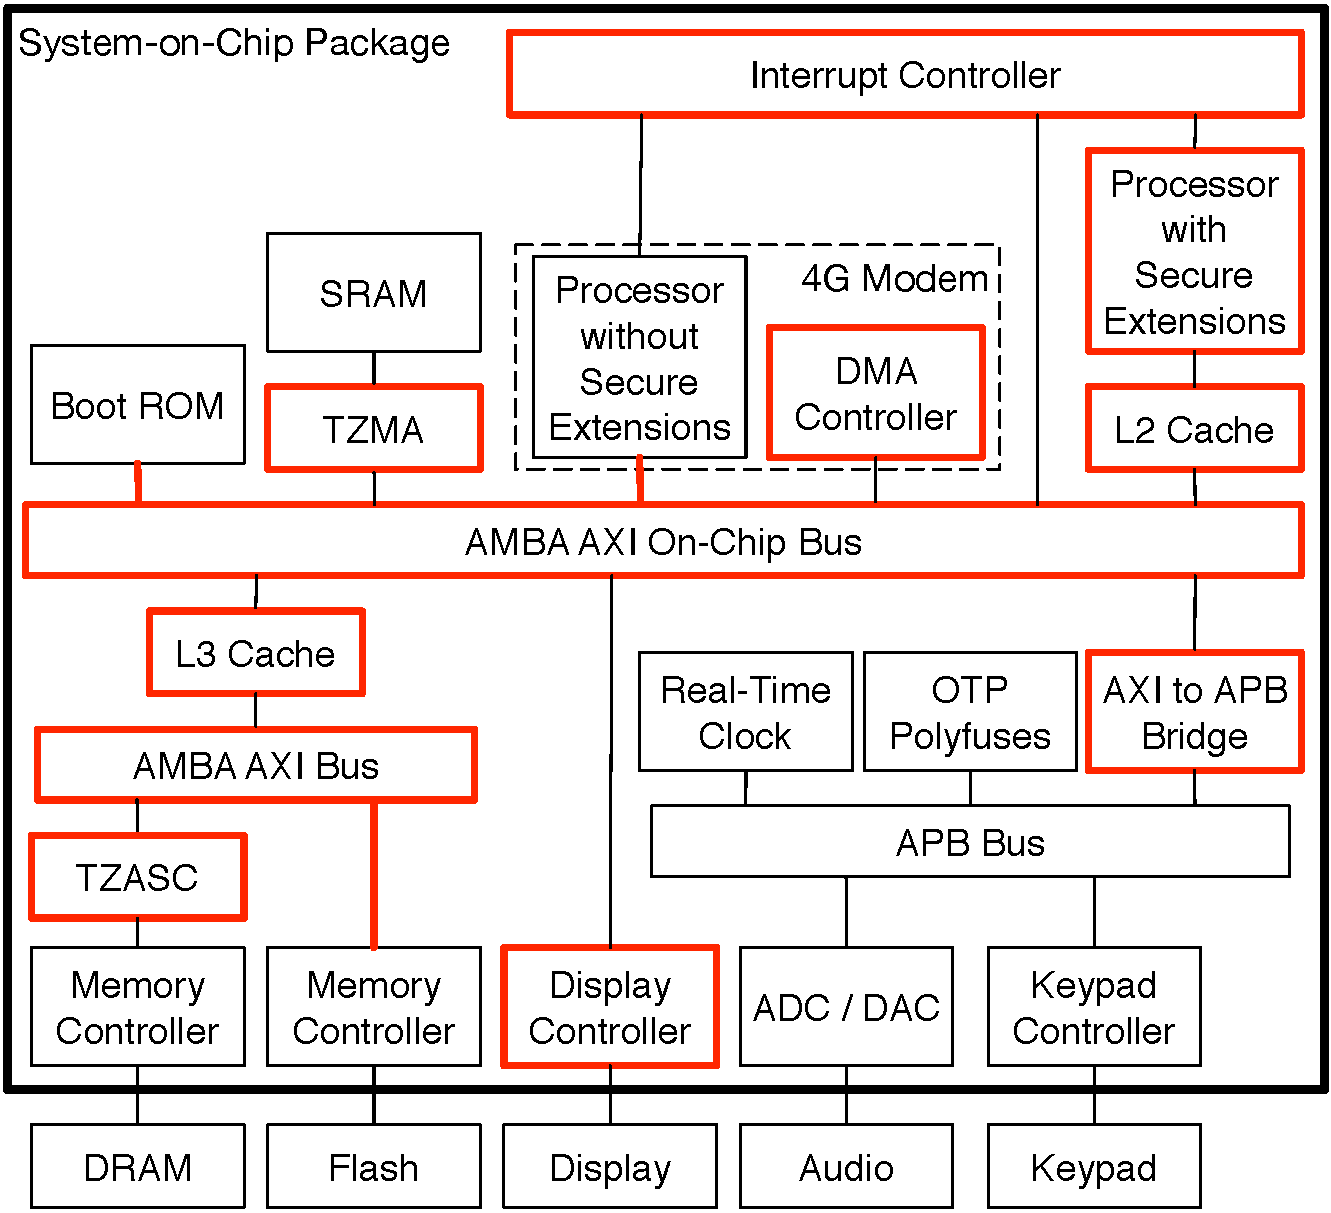
\includegraphics[width=85mm]{figures/trustzone.pdf}
  \caption{
    Smart SoC design based on TrustZone. The red IP blocks are TrustZone-aware.
    The red connections ignore the TrustZone secure bit in the bus address.
    Defining the system's security properties requires a complete understanding
    of all the red elements in this figure.
  }
  \label{fig:trustzone}
\end{figure}

TrustZone extends the address lines in the AMBA AXI system
bus~\cite{arm2004ambaxi} with one signal that indicates whether an access
belongs to the secure or normal (non-secure) world. ARM processor cores that
include TrustZone's ``Security Extensions'' can switch between executing code
in the normal world and code in the secure world. The address in each bus
access executed by a core reflects the world that the core is currently
executed.

The reset circuitry in a TrustZone processor places it in secure mode, and
points it to the first-stage bootloader stored in on-chip ROM. TrustZone's TCB
includes this bootloader, which initializes the platform, sets up the TrustZone
hardware to protect the secure container from untrusted software, and loads the
normal world's bootloader. The secure container must also implement a monitor
that performs the context switches needed to transition an execution core
between the two worlds. The monitor must also handle hardware exceptions, such
as interrupts, and route them to the appropriate world.

The TrustZone design gives the secure world's monitor unrestricted acces to the
normal world, so the monitor can implement inter-process communication (IPC)
between the software in the two worlds. Specifically, the monitor can issue
bus accesses using both secure and non-secure addresses. In general, the secure
world's software can compromise any level in the normal world's software stack.
For example, the secure container's software can jump into arbitrary locations
in the normal world by flipping a bit in a register. The untrusted software in
the normal world can only access the secure world via an instruction that jumps
into a well-defined location inside the monitor.

Conceptually, each TrustZone CPU core provides separate address translation
units for the secure and normal worlds. This is implemented by two page table
base registers, and by having the page walker use the page table base
corresponding to the core's current world. The physical addresses in the page
table entries are extended to include the values of the secure bit to be issued
on the AXI bus. The secure world is protected from untrusted software by having
the CPU core force the secure bit in the address translation result to zero for
normal world address translations. As the secure container manages its own page
tables, its memory accesses cannot be directly observed by the untrusted OS's
page fault handler.

TrustZone-aware hardware modules, such as caches, are trusted to use the secure
address bit in each bus access enforce the isolation between worlds. For
example, TrustZone's caches store the secure bit in the address tag for each
cache line, which effectively provides completely different views of the memory
space to the software running in different worlds. This design assumes that
memory space is partitioned between the two worlds, so no aliasing can occur.

The hardware modules that do not consume TrustZone's address bit are expected
to be connected to the AXI bus via IP cores that implement simple
partitioning techniques. For example, the TrustZone Memory Adapter (TZMA) can
be used to partition an on-chip ROM or SRAM into a secure region and a normal
region, and the TrustZone Address Space Controller (TZASC) partitions the
memory space provided by a DRAM controller into secure and normal regions. A
TrustZone-aware DMA controller rejects DMA transfers from the normal world that
reference secure world addresses.

It follows that analyzing the security properties of a TrustZone system
requires a precise understanding of the behavior and configuration of all the
hardware modules that are attached to the AXI bus. For example, the caches
described in TrustZone's documentation do not enforce a complete separation
between worlds, as they allow a world's memory accesses to evict the other
world's cache lines. This exposes the secure container software to cache timing
attacks from the untrusted software in the normal world. Unfortunately,
hardware manufacturers that license the TrustZone IP cores are reluctant to
disclose all the details of their designs, making it impossible for security
researchers to reason about TrustZone-based hardware.

The TrustZone components do not have any counter-measures for physical attacks.
However, a system that follows the recommendations in the TrustZone
documentation will not be exposed to physical attacks, under a threat model
that trusts the processor chip package. The AXI bus is designed to connect
components in a SoC design, so it cannot be tapped by an attacker. The
TrustZone documentation recommends having all the code and data in the secure
world stored in on-chip SRAM, which is not subjected to physical attacks.
However, this approach places significant limits on the secure container's
functionality, because on-chip SRAM is many orders of magnitude more expensive
than a DRAM chip of the same capacity.

TrustZone's documentation does not describe any software attestation
implementation. However, it does outline a method for implementing secure boot,
which comes down to having the first-stage bootloader verify a signature in the
second-stage bootloader against a public key whose cryptographic hash is burned
into on-chip \textit{One-Time Programmable} (OTP) polysilicon fuses. A hardware
measurement root can be built on top of the same components, by storing a
per-chip attestation key in the polyfuses, and having the first-stage
bootloader measure the second-stage bootloader and store its hash in an on-chip
SRAM region allocated to the secure world. The polyfuses would be gated by a
TZMA IP block that only makes them accessible to the secure world.

\HeadingLevelB{The XOM Architecture}

The execute-only memory (XOM) architecture \cite{lie2000xom} introduced the
approach of executing sensitive code and data in isolated containers managed by
untrusted host software. XOM outlined the mechanisms needed to isolate a
container's data from its untrusted software environment, such as saving the
register state to a protected memory area before servicing an interrupt.

XOM supports multiple containers by tagging every cache line with the
identifier of the container owning it, and ensures isolation by disallowing
memory accesses to cache lines that don't match the current container's
identifier. The operating system and the untrusted applications are considered
to belong to a container with a null identifier.

XOM also introduced the integration of encryption and HMAC functionality in
the processor's memory controller to protect container memory from physical
attacks on DRAM. The encryption and HMAC functionality is used for all cache
line evictions and fetches, and the ECC bits in DRAM chips are repurposed to
store HMAC values.

XOM's design cannot guarantee DRAM freshness, so the software in its containers
is vulnerable to physical replay attacks. Furthermore, XOM does not protect a
container's memory access patterns, meaning that any piece of malicious
software can perform cache timing attacks against the software in a container.
Last, XOM containers are destroyed when they encounter hardware exceptions,
such as page faults, so XOM does not support paging.

XOM predates the attestation scheme described above, and relies on a modified
software distribution scheme instead. Each container's contents are encrypted
with a symmetric key, which also serves as the container's identity. The
symmetric key, in turn, is encrypted with the public key of each CPU that is
trusted to run the container. A container's author can be assured that the
container is running on trusted software by embedding a secret into the
encrypted container data, and using it to authenticate the container. While
conceptually simpler than software attestation, this scheme does not allow the
container author to vet the container's software environment.

\HeadingLevelB{The Trusted Platform Module (TPM)}
\label{sec:sgx_related_tpm}

The Trusted Platform Module (TPM) \cite{grawrock2003tpm} introduced the
software attestation model described at the beginning of this section. The TPM
design does not require any hardware modifications to the CPU, and instead
relies on an auxiliary tamper-resistant chip. The TPM chip is only used to
store the attestation key and to perform software attestation. The TPM was
widely deployed on commodity computers, because it does not rely on CPU
modifications. Unfortunately, the cost of this approach is that the TPM has
very weak security guarantees, as explained below.

The TPM design provides one isolation container, covering all the software
running on the computer that has the TPM chip. It follows that the measurement
included in an attestation signature covers the entire OS kernel and all the
kernel modules, such as device drivers. However, commercial computers use a
wide diversity of devices, and their system software is updated at an
ever-increasing pace, so it is impossible to maintain a list of acceptable
measurement hashes corresponding to a piece of trusted software. Due to this
issue, the TPM's software attestation is not used in many security systems,
despite its wide deployment.

The TPM design is technically not vulnerable to any software attacks, because
it trusts all the software on the computer. However, a TPM-based system is
vulnerable to an attacker who has physical access to the machine, as the TPM
chip does not provide any isolation for the software on the computer.
Furthermore, the TPM chip receives the software measurements from the CPU,
so TPM-based systems are vulnerable to attackers who can tap the communication
bus between the CPU and the TPM.

Last, the TPM's design relies on the software running on the CPU to report its
own cryptographic hash. The TPM chip resets the measurements stored in Platform
Configuration Registers (PCRs) when the computer is rebooted. Then, the TPM
expects the software at each boot stage to cryptographically hash the software
at the next stage, and send the hash to the TPM. The TPM updates the PCRs to
incorporate the new hashes it receives, as shown in
Figure~\ref{fig:tpm_measurement}. Most importantly, the PCR value at any point
reflects all the software hashes received by the TPM up to that point. This
makes it impossible for software that has been measured to ``remove'' itself
from the measurement.

\begin{figure}[hbt]
  \centering
  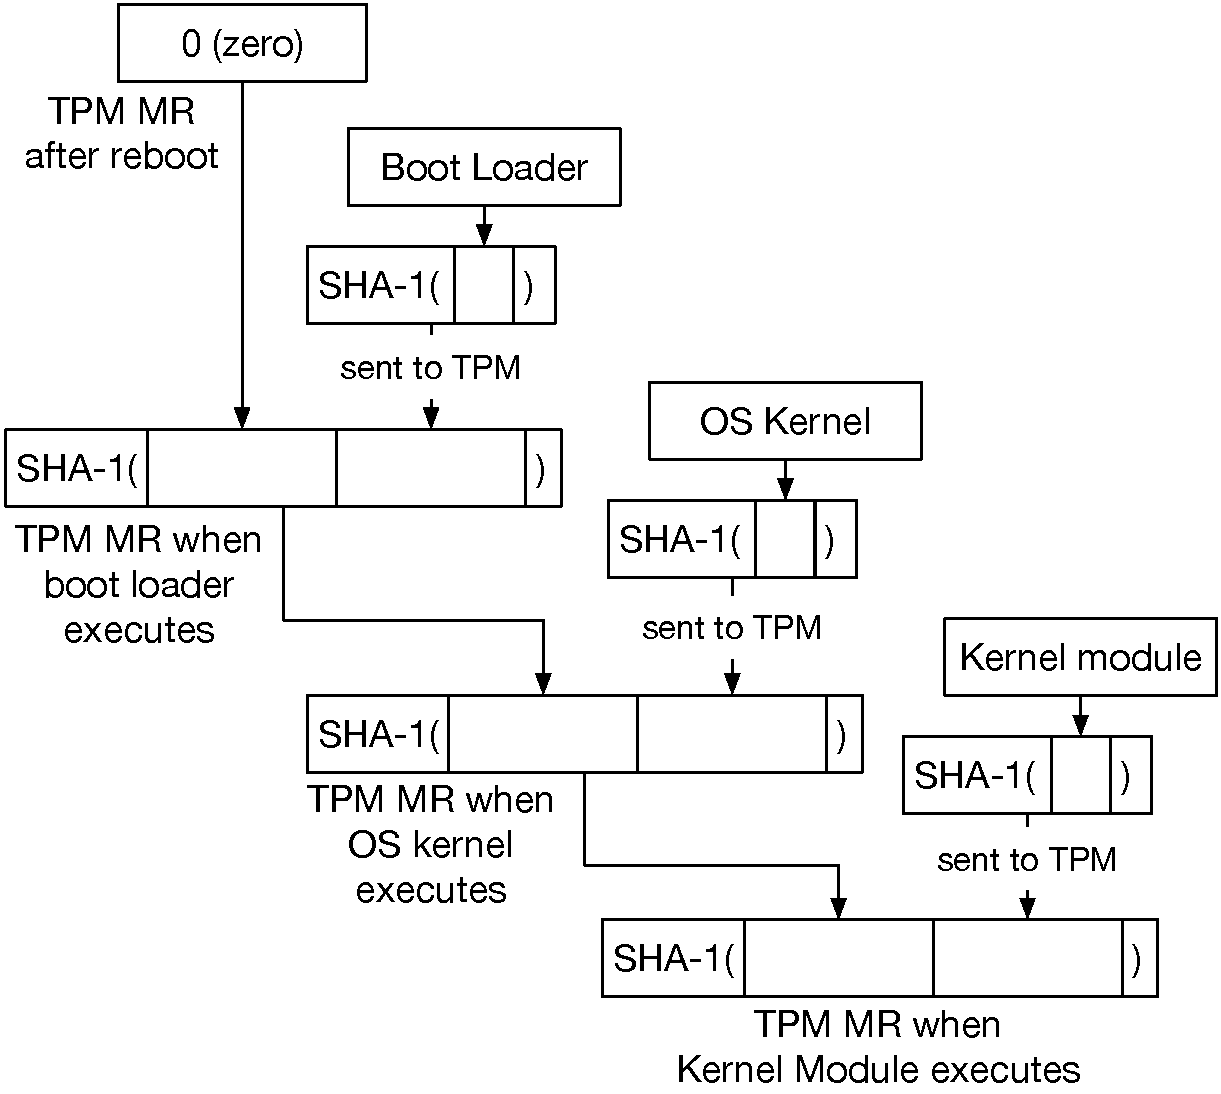
\includegraphics[width=85mm]{figures/tpm_measurement.pdf}
  \caption{
    The measurement stored in a TPM platform configuration register (PCR). The
    PCR is reset when the system reboots. The software at every boot stage
    hashes the next boot stage, and sends the hash to the TPM. The PCR's new
    value incorporates both the old PCR value, and the new software hash.
  }
  \label{fig:tpm_measurement}
\end{figure}

For example, the firmware on most modern computers implements the platform
initialization process in the Unified Extensible Firmware Interface (UEFI)
specification~\cite{forum2015uefi}. Each platform initialization phase is
responsible for verifying or measuring the firmware that implements the next
phase. The SEC firmware initializes the TPM PCR, and then stores the PEI's
measurement into a measurement register. In turn, the PEI implementation
measures the DXE firmware and updates the measurement register that stores the
PEI hash to account for the DXE hash. When the OS is booted, the hash in the
measurement register accounts for all the firmware that was used to boot the
computer.

Unfortunately, the security of the whole measurement scheme hinges on the
requirement that the first hash sent to the TPM must reflect the software that
runs in the first boot stage. The TPM threat model explicitly acknowledges this
issue, and assumes that the firmware responsible for loading the first stage
bootloader is securely embedded in the motherboard. However, virtually every
TPM-enabled computer stores its firmware in a flash memory chip that can be
re-programmed in software (\S~\ref{sec:motherboard}), so the TPM's measurement
can be subverted by an attacker who can reflash the computer's firmware
\cite{butterworth2013bios}.

On very recent Intel processors, the attack described above can be defeated by
having the initialization microcode (\S~\ref{sec:microcode_sec}) hash the
computer's firmware (specifically, the PEI code in UEFI \cite{forum2015uefi}
firwmare) and communicate the hash to the TPM chip. This is marketed as the
Measured Boot feature of Intel's Boot Guard \cite{ruan2014intelme}.

Sadly, most computer manufacturers use Verified Boot (also known as ``secure
boot'') instead of Measured Boot (also known as ``trusted boot''). Verified
Boot means that the processor's microcode only boots into PEI firmware that
contains a signature produced by a key burned into the chip's e-fuses. Verified
Boot does not impact the measurements stored on the TPM, so it does not improve
the security of software attestation.

\subsection{Intel's Trusted Execution Technology (TXT)}

Intel's Trusted Execution Technology (TXT) \cite{grawrock2009txt} uses the
TPM's software attestation model and auxilliary tamper-resistant chip, but
reduces the software inside the secure container to a virtual machine (guest
operating system and application) hosted by the CPU's hardware virtualization
features (VMX \cite{uhlig2005vmx}).

TXT isolates the software inside the container from untrusted software by
ensuring that the container has exclusive control over the entire computer
while it is active. This is accomplished by a secure initialization
authenticated code module (SINIT ACM) that effectively performs a warm system
reset before starting the container's VM.

TXT does not implement DRAM encryption or HMACs, and therefore is vulnerable to
physical DRAM attacks, just like TPM-based designs. Furthermore, early TXT
implementations were vulnerable to attacks where a malicious operating system
would program a device, such as a network card, to perform DMA transfers
to the DRAM region used by a TXT container \cite{wojtczuk2009txt,
wojtczuk2009txt2}. In recent Intel CPUs, the memory controller is integrated on
the CPU die, so the SINIT ACM
can securely set up the memory controller to reject DMA transfers targeting TXT
memory.

Early TXT implementations did not measure the SINIT ACM. Instead, the microcode
implementing the TXT launch instruction verified that the code module contained
an RSA signature by a hard-coded Intel key. SINIT ACM signatures cannot be
revoked if vulnerabilities are found, so TXT's software attestation had to be
revised when SINIT ACM exploits \cite{wojtczuk2011txt} surfaced. Currently, the
SINIT ACM's cryptographic hash is included in the attestation measurement.

Last, the warm reset performed by the SINIT ACM does not include the software
running in System Management Mode (SMM). SMM was designed
solely for the use of firmware, and is stored in a protected memory area
(SMRAM) which should not be accessible to non-SMM software. However, the SMM
handler was compromised on multiple occasions \cite{duflot2006smm,
rutkowska2008remap, wojtczuk2009smm, wecherowski2009smm, embleton2010smm}, and
an attacker that obtains SMM execution can access the memory used by TXT's
container.

\subsection{The Aegis Secure Processor}

The Aegis secure processor \cite{suh2003aegis} argued that Physically
Uncloneable Functions (PUFs) \cite{gassend2002puf} can be used to endow a
secure processor with a tamper-resistant private key, which is required for
software attestation. PUFs do not have the fabrication process drawbacks of
EEPROM, and are significantly more resilient to physical attacks than e-fuses.
Aegis relies on a security kernel in the operating system to isolate
containers, and includes the kernel's cryptographic hash in the measurement
reported by the software attestation signature.

Aegis relies on a trusted security kernel to isolate each container from the
other software on the computer by configuring the page tables used in address
translation. The security kernel is a subset of a typical OS kernel, and
handles virtual memory management, processes, and hardware exceptions. As the
security kernel is a part of the \textit{trusted code base} (TCB), its
cryptographic hash is included in the software attestation measurement. The
security kernel uses processor features to isolate itself from the untrusted
part of the operatings system, such as device drivers.

The Aegis memory controller encrypts the cache lines in one memory range, and
HMACs the cache lines in one other memory range. The two memory ranges can
overlap, and are configurable by the security kernel. Thanks to the two ranges,
the memory controller can avoid the latency overhead of cryptographic
operations for the DRAM outside containers. Aegis is not vulnerable to physical
replay attacks, as it uses a Merkle tree construction \cite{gassend2003merkle}
to guarantee DRAM freshness. The latency overhead of the Merkle tree is greatly
reduced by augmenting the L2 cache with the tree nodes for the cache lines.

Aegis' security kernel allows the OS to page out container memory, but verifies
the correctness of the paging operations. The security kernel uses the same
encryption and Merkle tree algorithms as the memory controller to guarantee the
privacy and integrity of the container pages that are swapped out from DRAM.
As the OS is free to page out container memory, it can learn a containter's
memory access patterns, at page granularity. Aegis containers are also
vulnerable to cache timing attacks.

\HeadingLevelB{The Bastion Architecture}
\label{sec:sgx_related_bastion}

The Bastion architecture \cite{champagne2010bastion} introduced the use of a
trusted hypervisor to provide secure containers to applications running inside
unmodified, untrusted operating systems. Bastion's hypervisor ensures that the
operating system does not interfere with the secure containers. We only
describe Bastion's virtualization extensions to architectures that use nested
page tables, like Intel's VMX \cite{uhlig2005vmx}.

The hypervisor enforces the containers' desired memory mappings in the OS page
tables, as follows. Each Bastion container has a Security Segment that lists
the virtual addresses and permissions of all the container's pages, and the
hypervisor maintains a Module State Table that stores an inverted page map,
associating each physical memory page to its container and virtual address. The
processor's hardware page walker is modified to invoke the hypervisor on every
TLB miss, before updating the TLB with the address translation result. The
hypervisor checks that the virtual address used by the translation matches the
expected virtual address associated with the physical address in the Module
State Table.

Bastion's cache lines are not tagged with container identifiers. Instead, only
TLB entries are tagged. The hypervisor's TLB miss handler sets the container
identifier for each TLB entry as it is created. Similarly to XOM and Aegis, the
secure processor checks the TLB tag against the current container's identifier
on every memory access.

Bastion offers the same protection against physical DRAM attacks as Aegis does,
without the restriction that a container's data must be stored inside a
continuous DRAM range. This is accomplished by extending cache lines and TLB
entries with flags that enable memory encryption and HMACing. The hypervisor's
TLB miss handler sets the flags on TLB entries, and the flags are propagated to
cache lines on memory writes.

The Bastion hypervisor allows the untrusted operating system to evict secure
container pages. The evicted pages are encrypted, HMACed, and covered by a
Merkle tree maintained by the hypervisor. Thus, the hypervisor ensures the
privacy, authenticity, and freshness of the swapped pages. However, the ability
to freely evict container pages allows a malicious OS to learn a container's
memory accesses with page granularity. Furthermore, Bastion's threat model
excludes cache timing attacks.

Bastion does not trust the platform's firmware, and computes the cryptographic
hash of the hypervisor after the firmware finishes playing its part in the
booting process. The hypervisor's hash is included in the measurement reported
by software attestation.

Intel's Software Guard Extensions (SGX)~\cite{mckeen2013sgx, anati2013sgx,
hoekstra2013sgx} implements secure containers for applications without making
any modifications to the processor's critical execution path. SGX does not
trust any layer in the computer's software stack (firmware, hypervisor, OS).
Instead, SGX's TCB consists of the CPU's microcode and a few privileged
containers. SGX introduces an approach to solving some of the issues raised by
multi-core processors with a shared, coherent last-level cache.

SGX does not extend caches or TLBs with container identity bits, and does not
require any security checks during normal memory accesses. As suggested in the
TrustZone documentation, SGX always ensures that a core's TLBs only contain
entries for the container that it is executing, which requires flushing the CPU
core's TLBs when context-switching between containers and untrusted software.

SGX follows Bastion's approach of having the untrusted OS manage the page
tables used by secure containers. The containers' security is preserved by a
TLB miss handler that relies on an inverted page map (the EPCM) to reject
address translations for memory that does not belong to the current container.

Like Bastion, SGX allows the untrusted operating system to evict secure
container pages, in a controlled fashion. After the OS initiates a container
page eviction, it must prove to the SGX implementation that it also switched
the container out of all cores that were executing its code, effectively
performing a very coarse-grained TLB shootdown.

SGX's microcode ensures the confidentiality, authenticity, and freshness of
each container's evicted pages, like Bastion's hypervisor. However, SGX relies
on a version-based Merkle tree, inspired by Aegis \cite{suh2003aegis}, and adds
an innovative twist that allows the operating system to dynamically shape the
Merkle tree. SGX also shares Bastion's and Aegis' vulnerability to memory
access pattern leaks, namely a malicious OS can directly learn a container's
memory accesses at page granularity, and any piece of software can perform
cache timing attacks.

SGX's software attestation is implemented using Intel's Enhanced Privacy ID
(EPID) group signature scheme \cite{brickell2009epid}, which is too complex for
a microcode implementation. Therefore, SGX relies on an assortment of
privileged containers that receive direct access to the SGX processor's
hardware keys. The privileged containers are signed using an Intel private key
whose corresponding public key is hard-coded into the SGX microcode, similarly
to TXT's SINIT ACM.

As SGX does not protect against cache timing attacks, the privileged enclave's
authors cannot use data-dependent memory accesses. For example, cache attacks
on the Quoting Enclave, which computes attestation signatures, would provide
an attack with a processor's EPID signing key and completely compromise SGX.

Intel's documentation states that SGX guarantees DRAM confidentiality,
authentication, and freshness by virtue of a Memory Encryption Engine (MEE).
The MEE is informally described in an ISCA 2015
tutorial~\cite{intel2015iscasgx}, and appears to lack a formal specification.
In the absence of further information, we assume that SGX provides the same
protection against physical DRAM attacks that Aegis and Bastion provide.

\HeadingLevelB{Sanctum}
\label{sec:related_sanctum}

Sanctum~\cite{costan2015sanctum} introduced a straightforward software/hardware
co-design that yields the same resilience against software attacks as SGX, and
adds protection against memory access pattern leaks, such as page fault
monitoring attacks and cache timing attacks.

Sanctum uses a conceptually simple cache partitioning scheme, where a
computer's DRAM is split into equally-sized continuous DRAM regions, and each
DRAM region uses distinct sets in the shared last-level cache (LLC). Each DRAM
region is allocated to exactly one container, so containers are isolated in
both DRAM and the LLC. Containers are isolated in the other caches by flushing
on context switches.

Like XOM, Aegis, and Bastion, Sanctum also considers the hypervisor, OS, and the
application software to conceptually belong to a separate container. Containers
are protected from the untrusted outside software by the same measures that
isolate containers from each other.

Sanctum relies on a trusted security monitor, which is the first piece of
firmware executed by the processor, and has the same security properties as
those of Aegis' security kernel. The monitor is measured by bootstrap code in
the processor's ROM, and its cryptographic hash is included in the software
attestation measurement. The monitor verifies the operating system's resource
allocation decisions. For example, it ensures that no DRAM region is ever
accessible to two different containers.

Each Sanctum container manages its own page tables mapping its DRAM regions,
and handles its own page faults. It follows that a malicious OS cannot learn the
virtual addresses that would cause a page fault in the container. Sanctum's
hardware modifications work in conjunction with the security monitor to make
sure that a container's page tables only reference memory inside the container's
DRAM regions.

The Sanctum design focuses completely on software attacks, and does not offer
protection from any physical attack. The authors expect Sanctum's hardware
modifications to be combined with the physical attack protections in Aegis or
Ascend.

\HeadingLevelB{Ascend and Phantom}

The Ascend \cite{fletcher2012ascend} and Phantom \cite{maas2013phantom} secure
processors introduced practical implementations of Oblivious RAM
\cite{goldreich1987oram} techniques in the CPU's memory controller. These
processors are resilient to attackers who can probe the DRAM address bus and
attempt to learn a container's private information from its DRAM memory access
pattern.

Implementing an ORAM scheme in a memory controller is largely orthogonal to the
other secure architectures described above. It follows, for example, that
Ascend's ORAM implementation can be combined with Aegis' memory encryption and
authentication, and with Sanctum's hardware extensions and security monitor,
yielding a secure processor that can withstand both software attacks and
physical DRAM attacks.


\section{SGX Programming Model}

The central concept of SGX is the \textit{enclave}, a protected environment
that contains the code and data pertaining to a security-sensitive computation.
SGX-enabled processors provide trusted computing by isolating each enclave's
environment from the untrusted software outside the enclave, and by
implementing a software attestation scheme that allows a remote party to
authenticate the software running inside an enclave. SGX's isolation mechanisms
are intended to protect the privacy and integrity of the computation performed
inside an enclave from attacks coming from malicious software executing on the
same computer, as well as from a limited set of physical attacks.

This section summarizes the SGX concepts that make up a mental model which is
sufficient for programmers to author SGX enclaves and to add SGX support to
existing system software. All the information in this section is backed up by
Intel's Software Developer Manual (SDM). Future sections use the model created
here to fill in some the missing pieces in the manual, namely a description of
the SGX implementation and an anlysis of SGX's security properties.


\HeadingLevelB{SGX Physical Memory Organization}
\label{sec:sgx_prm}

% Intel SGX Resource Enumeration Leaves: SDM S 37.7.2
% Interactions with DMA: SDM S 42.10, SGX2 S 6.10

The enclaves' code and data is stored in \textit{Processor Reserved Memory}
(PRM), which is a subset of DRAM that cannot be directly accessed by other
software, including system software and SMM code. The CPU's integrated memory
controllers (\S~\ref{sec:cpu_die}) also reject DMA transfers targeting the PRM,
thus protecting it from access by other peripherals.

% EPC and Management of EPC Pages: SGX2 S 3.5
% Interactions with Memory Configuration: SGX2 S 6.11
% Memory Type Considerations for PRMRR: SGX2 S 6.11.1
% Interactions of PRMRR with Physical Memory Accesses: SGX2 S 6.11.3.1

The PRM is a continuous range of memory whose bounds are configured using a
base and a mask register with the same semantics as a variable memory type
range~(\S~\ref{sec:cacheability_config}). Therefore, the PRM's size must be an
integer power of two, and its start address must be aligned to the same power
of two. Due to these restrictions, checking if an address belongs to the PRM
can be done very cheaply in hardware, using the circuit outlined in
\S~\ref{sec:cacheability_config}.

The SDM does not describe the PRM and the PRM range registers (PRMRR). These
concepts are documented in the SGX
manuals~\cite{intel2013sgxmanual, intel2014sgx2manual} and in one of the SGX
papers~\cite{mckeen2013sgx}. Therefore, the PRM is a micro-architectural detail
that might change in future implementations of SGX. Our security analysis of
SGX relies on implementation details surrounding the PRM, and will have to be
re-evaluated for SGX future implementations.


\HeadingLevelC{The Enclave Page Cache (EPC)}
\label{sec:sgx_epc}

% Enclave Page Cache: SDM S 37.5
% EPC and Management of EPC Pages: SDM S 39.5, S 39.5.1

The contents of enclaves and the associated data structures are stored in the
\textit{Enclave Page Cache} (EPC), which is a subset of the PRM, as shown in
Figure~\ref{fig:sgx_epc}.

\begin{figure}[hbt]
  \centering
  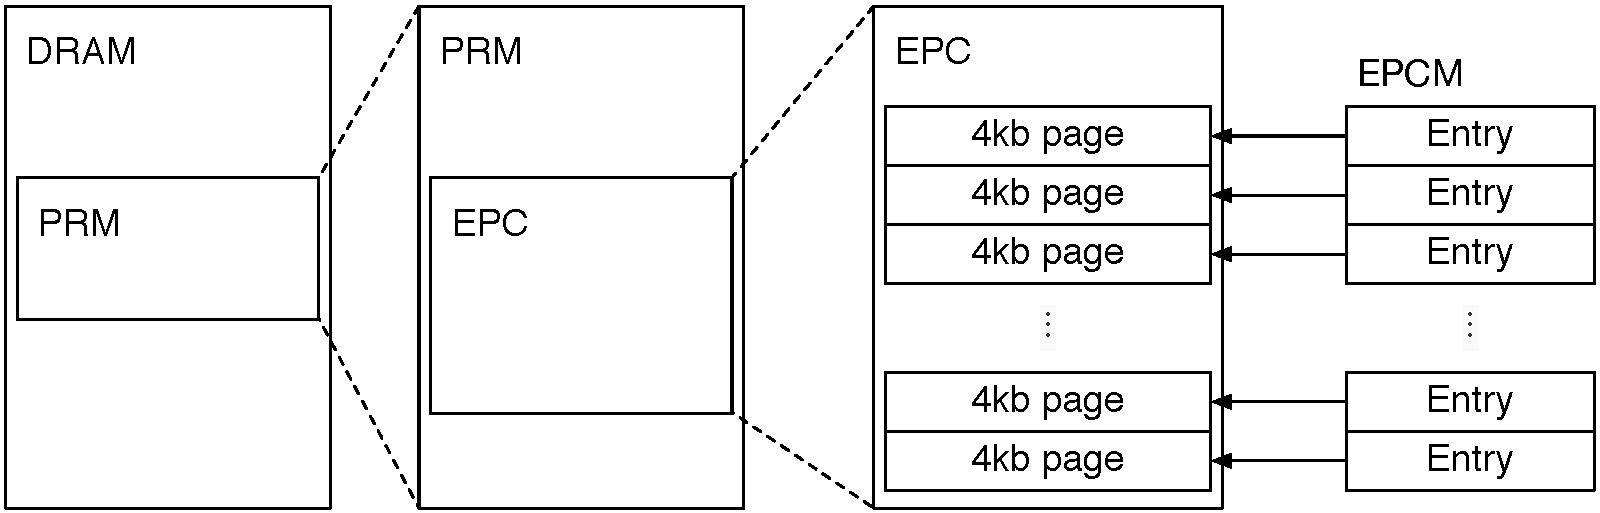
\includegraphics[width=87mm]{figures/sgx_epc.pdf}
  \caption{
    Enclave data is stored into the EPC, which is a subset of the PRM. The
    PRM is a contiguous range of DRAM that cannot be accessed by system
    software or peripherals.
  }
  \label{fig:sgx_epc}
\end{figure}

The SGX design supports having multiple enclaves on a system at the same time,
which is a necessity in multi-process environments. This is achieved by having
the EPC split into 4~KB pages that can be assigned to different enclaves. The
EPC uses the same page size as the architecture's address translation feature
(\S~\ref{sec:paging}). This is not a coincidence, as future sections will
reveal that the SGX implementation is tightly coupled with the address
translation implementation.

The EPC is managed by the same system software that manages the rest of the
computer's physical memory. The system software, which can be a hypervisor or
an OS kernel, uses SGX instructions to allocate unused pages to enclaves, and
to free previously allocated EPC pages. The system software is expected to
expose enclave creation and management services to application software.

Non-enclave software cannot directly access the EPC, as it is contained in the
PRM. This restriction plays a key role in SGX's enclave isolation guarantees,
but creates an obstacle when the system software needs to load the initial code
and data into a newly created enclave. The SGX design solves this problem by
having the instructions that allocate an EPC page to an enclave also initialize
the page. Most EPC pages are initialized by copying data from a non-PRM memory
page.


\HeadingLevelC{The Enclave Page Cache Map (EPCM)}
\label{sec:sgx_epcm}

% Enclave Page Cache Map (EPCM): SDM S 37.5.1, SDM S 38.19
% SECINFO.FLAGS: SDM S 38.11.1
% PAGE_TYPE Field Definition: SDM S 38.11.2

The SGX design expects the system software to allocate the EPC pages to
enclaves. However, as the system software is not trusted, SGX processors check
the correctness of the system software's allocation decisions, and refuse to
perform any action that would compromise SGX's security guarantees. For
example, if the system software attempts to allocate the same EPC page to two
enclaves, the SGX instruction used to perform the allocation will fail.

In order to perform its security checks, SGX records some information about the
system software's allocation decisions for each EPC page in the
\textit{Enclave Page Cache Map}~(EPCM). The EPCM is an array with one entry
per EPC page, so computing the address of a page's EPCM entry only requires a
bitwise shift operation and an addition.

The EPCM's contents is only used by SGX's security checks. Under normal
operation, the EPCM does not generate any software-visible behavior, and
enclave authors and system software developers can mostly ignore it.
Therefore, the SDM only describes the EPCM at a very high level, listing the
information contained within and noting that the EPCM is ``trusted memory''.
The SDM does not disclose the storage medium or memory layout used by the EPCM.

The EPCM uses the information in Table~\ref{fig:sgx_epcm_ownership_fields} to
track the ownership of each EPC page. We defer a full discussion of the EPCM to
a later section, because its contents is intimately coupled with all of SGX's
features, which will be described over the next few sections.

\begin{table}[hbt]
  \centering
  \begin{tabularx}{\columnwidth}{| l | r | X |}
  \hline
  \textbf{Field} & \textbf{Bits} & \textbf{Description}\\
  \hline
  VALID & 1 & 0 for un-allocated EPC pages \\
  \hline
  PT & 8 & page type \\
  \hline
  ENCLAVESECS &  & identifies the enclave owning the page \\
  \hline
  \end{tabularx}
  \caption{
    The fields in an EPCM entry that track the ownership of pages.
  }
  \label{fig:sgx_epcm_ownership_fields}
\end{table}

The SGX instructions that allocate an EPC page set the VALID bit of the
corresponding EPCM entry to 1, and refuse to operate on EPC pages whose VALID
bit is already set.

The instruction used to allocate an EPC page also determines the page's
intended usage, which is recorded in the \textit{page type} (PT) field of the
corresponding EPCM entry. The pages that store an enclave's code and data are
considered to have a \textit{regular} type (PT\_REG in the SDM). The pages
dedicated to the storage of SGX's supporting data structures are tagged with
special types. For example, the PT\_SECS type identifies pages that hold SGX
Enclave Control Structures, which will be described in the following section.
The other EPC page types will be described in future sections.

Last, a page's EPCM entry also identifies the enclave that owns the EPC page.
This information is used by the mechanisms that enforce SGX's isolation
guarantees to prevent an enclave from accessing another enclave's private
information. As the EPCM identifies a single owning enclave for each EPC page,
it is impossible for enclaves to communicate via shared memory using EPC pages.
Fortunately, enclaves can share untrusted non-EPC memory, as will be discussed
in \S~\ref{sec:sgx_paging}.


\HeadingLevelC{The SGX Enclave Control Structure (SECS)}
\label{sec:sgx_secs}

% Data Structures and Enclave Operation: SDM S 37.4
% SGX Enclave Control Structure (SECS): SDM S 38.7, S 38.7.1

SGX stores per-enclave metadata in a
\textit{SGX Enclave Control Structure}~(SECS) associated with each enclave.
Each SECS is stored in a dedicated EPC page with the page type PT\_SECS. These
pages are not intended to be mapped into any enclave's address space, and are
exclusively used by the CPU's SGX implementation.

% Constructing an Enclave: SDM S 39.1
% ECREATE: SDM S 39.1.1, S 41.3
% Implicit vs. Explicit accesses: SDM S 38.5.3
% Implicit accesses: SDM S 38.5.3.2

An enclave's identity is almost synonymous to its SECS. The first step in
bringing an enclave to life allocates an EPC page to serve as the enclave's
SECS, and the last step in destroying an enclave deallocates the page holding
its SECS. The EPCM entry field identifying the enclave that owns an EPC page
points to the enclave's SECS. The system software uses the virtual address of
an enclave's SECS to identify the enclave when invoking SGX instructions.

% Access Control Requirements: SDM S 38.3

All SGX instructions take virtual addresses as their inputs. Given that SGX
instructions use SECS addresses to identify enclaves, the system software must
create entries in its page tables pointing to the SECS of the enclaves it
manages. However, the system software cannot access any SECS page, as these
pages are stored in the PRM. SECS pages are not intended to be mapped inside
their enclaves' virtual address spaces, and SGX-enabled processors explicitly
prevent enclave code from accessing SECS pages.

% SGX Enclave Control Structure (SECS): SDM S 38.7, S 38.7.1

This seemingly arbitrary limitation is in place so that the SGX implementation
can store sensitive information in the SECS, and be able to assume that no
potentially malicious software will access that information. For example, the
SDM states that each enclave's measurement is stored in its SECS. If software
would be able to modify an enclave's measurement, SGX's software attestation
scheme would provide no security assurances.

The SECS is strongly coupled with many of SGX's features. Therefore, the pieces
of information that make up the SECS will be gradually introduced as the
different aspects of SGX are described.

\subsection{The Memory Layout of an SGX Enclave}
\label{sec:sgx_enclave_layout}

SGX was designed to minimize the effort required to convert application code to
take advantage of enclaves. History suggests this is a wise decision, as a
large factor in the continued dominance of the Intel architecture is its
ability to maintain backward compatibility. To this end, SGX enclaves were
designed to be conceptually similar to the leading software modularization
construct, dynamically loaded libraries, which are packaged as \texttt{.so}
files on Unix, and \texttt{.dll} files on Windows.

For simplicity, we describe the interaction between enclaves and non-enclave
software assuming that each enclave is used by exactly one application process,
which we shall refer to as the enclave's \textit{host process}. We do note,
however, that the SGX design does not explicitly prohibit multiple application
processes from sharing an enclave.


\subsubsection{The Enclave Linear Address Range (ELRANGE)}
\label{sec:sgx_elrange}

% SGX Enclave Control Structure (SECS): SDM S 38.7

Each enclave designates an area in its virtual address space, called the
\textit{enclave linear address range} (ELRANGE), which is used to map the code
and the sensitive data stored in the enclave's EPC pages. The virtual address
space outside ELRANGE is mapped to access non-EPC memory via the same virtual
addresses as the enclave's host process, as shown in
Figure~\ref{fig:sgx_elrange}.

\begin{figure}[hbt]
  \centering
  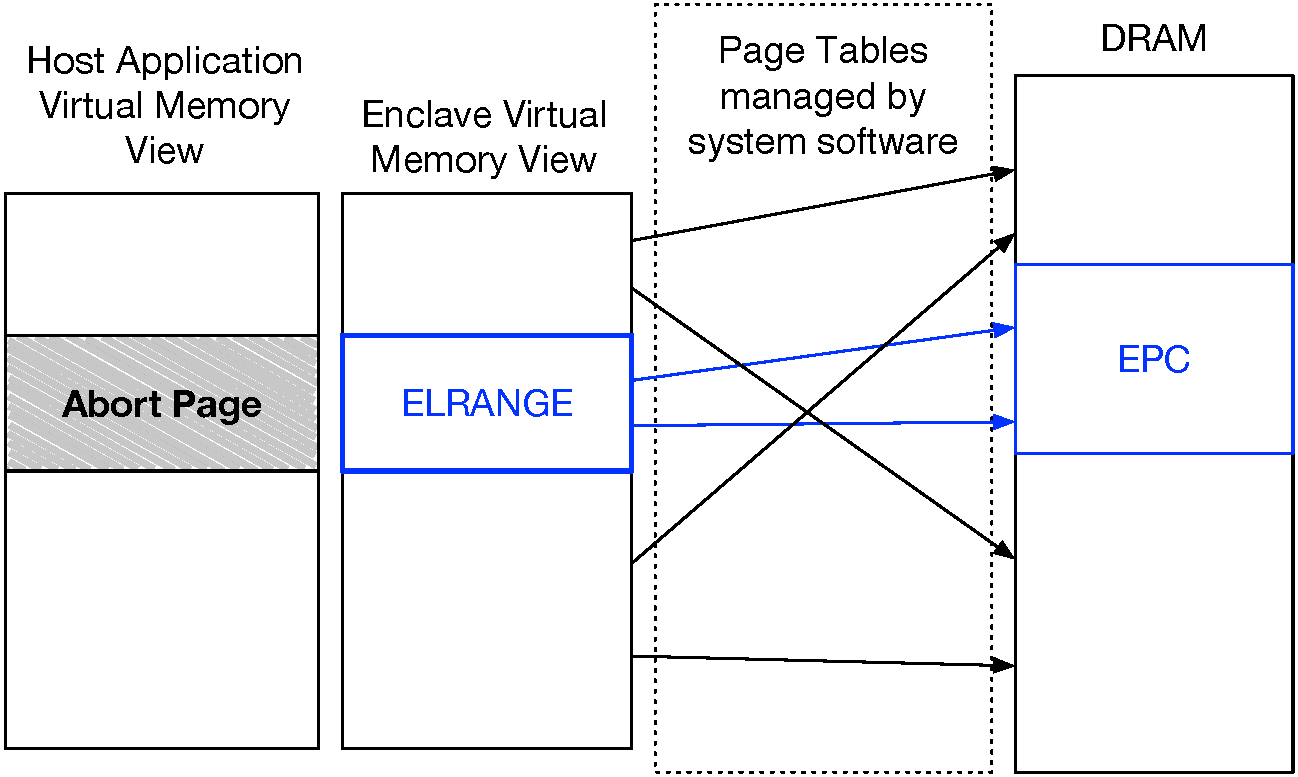
\includegraphics[width=85mm]{figures/sgx_elrange.pdf}
  \caption{
    An enclave's EPC pages are accessed using a dedicated region in the
    enclave's virtual address space, called ELRANGE. The rest of the virtual
    address space is used to access the memory of the host process. The memory
    mappings are established using the page tables managed by system software.
  }
  \label{fig:sgx_elrange}
\end{figure}

The SGX design guarantees that the enclave's memory accesses inside ELRANGE
obey the virtual memory abstraction~(\S~\ref{sec:paging_concepts}), while
memory accesses outside ELRANGE receive no guarantees. Therefore, enclaves must
store all their code and private data inside ELRANGE, and must consider the
memory outside ELRANGE to be an untrusted interface to the outside world.

The word ``linear'' in ELRANGE references the linear addresses produced by the
vestigial segmentation feature~(\S~\ref{sec:segments}) in the 64-bit Intel
architecture. For most purposes, ``linear'' can be treated as a synonym for
``virtual''.

ELRANGE is specified using a base (the BASEADDR field) and a size (the SIZE)
in the enclave's SECS~(\S~\ref{sec:sgx_secs}). ELRANGE must meet the same
constraints as a variable memory type range (\S~\ref{sec:cacheability_config})
and as the PRM range~(\S~\ref{sec:sgx_prm}), namely the size must be a power of
2, and the base must be aligned to the size. These restrictions are in place so
that the SGX implementation can inexpensively check whether an address belongs
to an enclave's ELRANGE, in either hardware~(\S~\ref{sec:cacheability_config})
or software.

When an enclave represents a dynamic library, it is natural to set ELRANGE to
the memory range reserved for the library by the loader. The ability to access
non-enclave memory from enclave code makes it easy to reuse existing library
code that expects to work with pointers to memory buffers managed by code in the
host process.


\subsubsection{SGX Enclave Attributes}
\label{sec:sgx_secs_attributes}

The execution environment of an enclave is heavily influenced by the value of
the ATTRIBUTES field in the enclave's SECS~(\S~\ref{sec:sgx_secs}). The rest of
this work will refer to the field's sub-fields, shown in
Table~\ref{fig:sgx_secs_attributes}, as \textit{enclave attributes}.

% ATTRIBUTES: SDM S 37.8.1

\begin{table}[hbt]
  \centering
  \begin{tabularx}{\columnwidth}{| l | r | X |}
  \hline
  \textbf{Field} & \textbf{Bits} & \textbf{Description} \\
  \hline
  DEBUG & 1 & Opts into enclave debugging features. \\
  \hline
  XFRM & 64 & The value of XCR0~(\S~\ref{sec:registers}) while this enclave's
              code is executed. \\
  \hline
  MODE64BIT & 1 & Set for 64-bit enclaves. \\
  \hline
  \end{tabularx}
  \caption{
    An enclave's attributes are the sub-fields in the ATTRIBUTES field of the
    enclave's SECS. This table shows a subset of the attributes defined in the
    SGX documentation.
  }
  \label{fig:sgx_secs_attributes}
\end{table}

The most important attribute, from a security perspective, is the DEBUG flag.
When this flag is set, it enables the use of SGX's debugging features for this
enclave. These debugging features include the ability to read and modify most
of the enclave's memory. Therefore, DEBUG should only be set in a development
environment, as it causes the enclave to lose all the SGX security guarantees.

SGX guarantees that enclave code will always run with the XCR0
register~(\S~\ref{sec:registers}) set to the value indicated by
\textit{extended features request mask}~(XFRM). Enclave authors are expected to
use XFRM to specify the set of architectural extensions enabled by the compiler
used to produce the enclave's code. Having XFRM be explicitly specified allows
Intel to design new architectural extensions that change the semantics of
existing instructions, such as Memory Protection Extensions (MPX), without
having to worry about the security implications on enclave code that was
developed without an awareness of the new features.

The MODE64BIT flag is set to true for enclaves that use the 64-bit Intel
architecture. From a security standpoint, this flag should not even exist, as
supporting a secondary architecture adds unnecessary complexity to the SGX
implementation, and increases the probability that security vulnerabilities
will creep in. In the interest of mental sanity, this work does not analyze the
behavior of SGX for enclaves whose MODE64BIT flag is cleared. However, a
security researcher who wishes to find vulnerabilities in SGX might study this
area.

Last, the INIT flag is always false when the enclave's SECS is created. The
flag is set to true at a certain point in the enclave lifecycle, which will be
summarized in \S~\ref{sec:sgx_enclave_lifecycle}.


\subsubsection{Address Translation for SGX Enclaves}
\label{sec:sgx_paging}

% Access Control Requirements: SDM S 38.3
% Interactions with VMX: SDM S 42.5, S 42.5.{1,2,3,4,5}

Under SGX, the operating system and hypervisor are still in full control of the
page tables and EPTs, and each enclave's code uses the same address translation
process and page tables~(\S~\ref{sec:paging}) as its host application. This
minimizes the amount of changes required to add SGX support to existing system
software. At the same time, having the page tables managed by untrusted system
software opens SGX up to the address translation attacks described in
\S~\ref{sec:address_translation_attacks}. As future sections will reveal, a
good amount of the complexity in SGX's design can be attributed to the need to
prevent these attacks.

SGX's active memory mapping attacks defense mechanisms revolve around ensuring
that each EPC page can only be mapped at a specific virtual
address~(\S~\ref{sec:segments}). When an EPC page is allocated, its intended
virtual address is recorded in the EPCM entry for the page, in the ADDRESS
field.

When an address translation (\S~\ref{sec:paging}) result is the physical
address of an EPC page, the CPU ensures\footnote{A mismatch triggers a general
protection fault (\#GP, \S~\ref{sec:faults}).} that the virtual address given
to the address translation process matches the expected virtual address
recorded in the page's EPCM entry.

SGX also protects against some passive memory mapping attacks and fault
injection attacks by ensuring that the access permissions of each EPC page
always match the enclave author's intentions. The access permissions for each
EPC page are specified when the page is allocated, and recorded in the
\textit{readable}~(R), \textit{writable}~(W), and \textit{executable}~(X)
fields in the page's EPCM entry, shown in
Table~\ref{fig:sgx_epcm_access_fields}.

\begin{table}[hbt]
  \centering
  \begin{tabularx}{\columnwidth}{| l | r | X |}
  \hline
  \textbf{Field} & \textbf{Bits} & \textbf{Description}\\
  \hline
  ADDRESS & 48 & the virtual address used to access this page\\
  \hline
  R & 1 & allow reads by enclave code\\
  \hline
  W & 1 & allow writes by enclave code\\
  \hline
  X & 1 & allow execution of code inside the page, inside enclave\\
  \hline
  \end{tabularx}
  \caption{
    The fields in an EPCM entry that indicate the enclave's intended virtual
    memory layout.
  }
  \label{fig:sgx_epcm_access_fields}
\end{table}

When an address translation (\S~\ref{sec:paging}) resolves into an EPC page,
the corresponding EPCM entry's fields override the access permission attributes
(\S~\ref{sec:page_table_attributes}) specified in the page tables. For example,
the W field in the EPCM entry overrides the writable (W) attribute, and the X
field overrides the disable execution (XD) attribute.

It follows that an enclave author must include memory layout information along
with the enclave, in such a way that the system software loading the enclave
will know the expected virtual memory address and access permissions for each
enclave page. In return, the SGX design guarantees to the enclave authors that
the system software, which manages the page tables and EPT, will not be able to
set up an enclave's virtual address space in a manner that is inconsistent with
the author's expectations.

The \texttt{.so} and \texttt{.dll} file formats, which are SGX's intended
enclave delivery vehicles, already have provisions for specifying the virtual
addresses that a software module was designed to use, as well as the desired
access permissions for each of the module's memory areas.

Last, a SGX-enabled CPU will ensure that the virtual memory inside
ELRANGE~(\S~\ref{sec:sgx_elrange}) is mapped to EPC pages. This prevents the
system software from carrying out an address translation attack where it maps
the enclave's entire virtual address space to DRAM pages outside the PRM, which
do not trigger any of the checks above, and can be directly accessed by the
system software.


\subsubsection{The Thread Control Structure (TCS)}
\label{sec:sgx_tcs}

% Thread Control Structure (TCS): SDM S 38.8, S 38.8.{1,2,3,4}

The SGX design fully embraces multi-core processors. It is possible for
multiple logical processors~(\S~\ref{sec:cpu_die}) to concurrently execute the
same enclave's code at the same time, via different threads.

The SGX implementation uses a \textit{Thread Control Structure}~(TCS) for each
logical processor that executes an enclave's code. It follows that an enclave's
author must provision at least as many TCS instances as the maximum number of
concurrent threads that the enclave is intended to support.

Each TCS is stored in a dedicated EPC page whose EPCM entry type is PT\_TCS.
The SDM describes the first few fields in the TCS. These fields are considered
to belong to the architectural part of the structure, and therefore are
guaranteed to have the same semantics on all the processors that support SGX.
The rest of the TCS is not documented.

% Access Control Requirements: SDM S 38.3
% EDBGRD, EDBGWR: SDM S 41.3

The contents of an EPC page that holds a TCS cannot be directly accessed, even
by the code of the enclave that owns the TCS. This restriction is similar to the
restriction on accessing EPC pages holding SECS instances. However, the
architectural fields in a TCS can be read by enclave debugging instructions.

The architectural fields in the TCS lay out the context
switches~(\S~\ref{sec:registers}) performed by a logical processor when it
transitions between executing non-enclave and enclave code.

For example, the OENTRY field specifies the value loaded in the instruction
pointer (RIP) when the TCS is used to start executing enclave code, so the
enclave author has strict control over the entry points available to enclave's
host application. Furthermore, the OFSBASGX and OFSBASGX fields specify the
base addresses loaded in the FS and GS segment
registers~(\S~\ref{sec:segments}), which typically point to Thread Local
Storage (TLS).


\subsubsection{The State Save Area (SSA)}
\label{sec:sgx_ssa}

% Interactions with the Processor Extended State and Miscellaneous State:
%     SDM S 42.7
% Requirements and Architecture Overview: SDM S 42.7.1

% State Save Area (SSA) Frame: SDM S 38.9

When the processor encounters a hardware exception~(\S~\ref{sec:faults}), such
as an interrupt~(\S~\ref{sec:interrupts}), while executing the code inside an
enclave, it performs a privilege level switch (\S~\ref{sec:faults}) and invokes
a hardware exception handler provided by the system software. Before executing
the exception handler, however, the processor needs a secure area to store the
enclave code's execution context~(\S~\ref{sec:registers}), so that the
information in the execution context is not revealed to the untrusted system
software.

% Relevant Fields in Various Data Structures: SDM S 42.7.2
% SECS.SSAFRAMESIZE: SDM S 42.7.2.2

In the SGX design, the area used to store an enclave thread's execution context
while a hardware exception is handled is called a \texttt{State Save
Area}~(SSA), illustrated in Figure~\ref{fig:sgx_enclave_layout}. Each TCS
references a contiguous sequence of SSAs. The \textit{offset of the SSA
array}~(OSSA) field specifies the location of the first SSA in the enclave's
virtual address space. The \textit{number of SSAs}~(NSSA) field indicates the
number of available SSAs.

\begin{figure}[hbt]
  \centering
  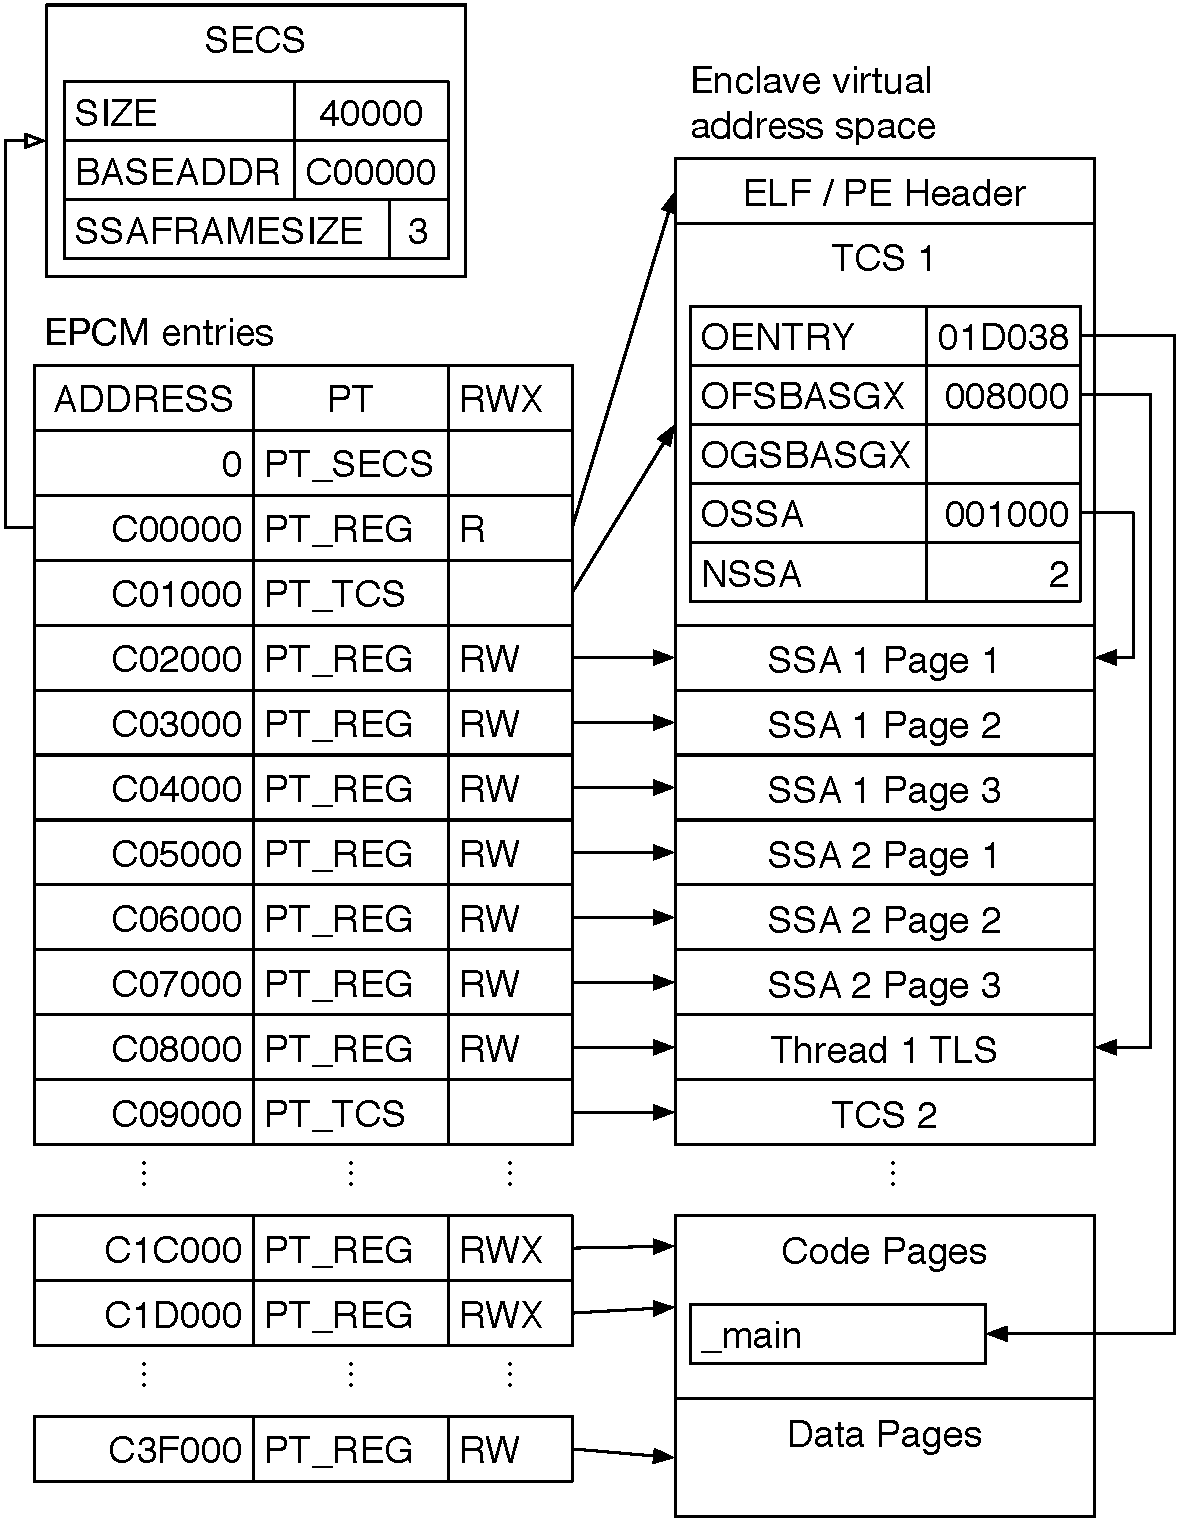
\includegraphics[width=85mm]{figures/sgx_enclave_layout.pdf}
  \caption{
    A possible layout of an enclave's virtual address space. Each enclave has a
    SECS, and one TCS per supported concurrent thread. Each TCS points to a
    sequence of SSAs, and specifies initial values for RIP and for the base
    addresses of FS and GS.
  }
  \label{fig:sgx_enclave_layout}
\end{figure}

Each SSA starts at the beginning of an EPC page, and uses up the number of EPC
pages that is specified in the SSAFRAMESIZE field of the enclave's SECS. These
alignment and size restrictions most likely simplify the SGX implementation by
reducing the number of special cases that it needs to handle.

% Relevant Fields in Various Data Structures: SDM S 42.7.2
% SECS.ATTRIBUTES.XFRM: SDM S 42.7.2.1

An enclave thread's execution context consists of the general-purpose registers
(GPRs) and the result of the XSAVE instruction~(\S~\ref{sec:registers}).
Therefore, the size of the execution context depends on the requested-feature
bitmap~(RFBM) used by to XSAVE. All the code in an enclave uses the same RFBM,
which is declared in the XFRM enclave
attribute~(\S~\ref{sec:sgx_secs_attributes}). The number of EPC pages reserved
for each SSA, specified in SSAFRAMESIZE,
must\footnote{\texttt{ECREATE}~(\S~\ref{sec:sgx_ecreate}) fails if SSAFRAMESIZE
is too small.} be large enough to fit the XSAVE output for the feature bitmap
specified by XFRM.

SSAs are stored in regular EPC pages, whose EPCM page type is PT\_REG.
Therefore, the SSA contents is accessible to enclave software. The SSA layout
is architectural, and is completely documented in the SDM. This opens up
possibilities for an enclave exception handler that is invoked by the host
application after a hardware exception occurs, and acts upon the information in
a SSA.

\subsection{The Life Cycle of an SGX Enclave}
\label{sec:sgx_enclave_lifecycle}

An enclave's life cycle is deeply intertwined with resource management,
specifically the allocation of EPC pages. Therefore, the instructions that
transition between different life cycle states can only be executed by the
system software. The system software is expected to expose the SGX instructions
described below as enclave loading and teardown services.

The following subsections describe the major steps in an enclave's lifecycle,
which is illustrated by Figure~\ref{fig:sgx_enclave_lifecycle}.

\begin{figure}[hbt]
  \centering
  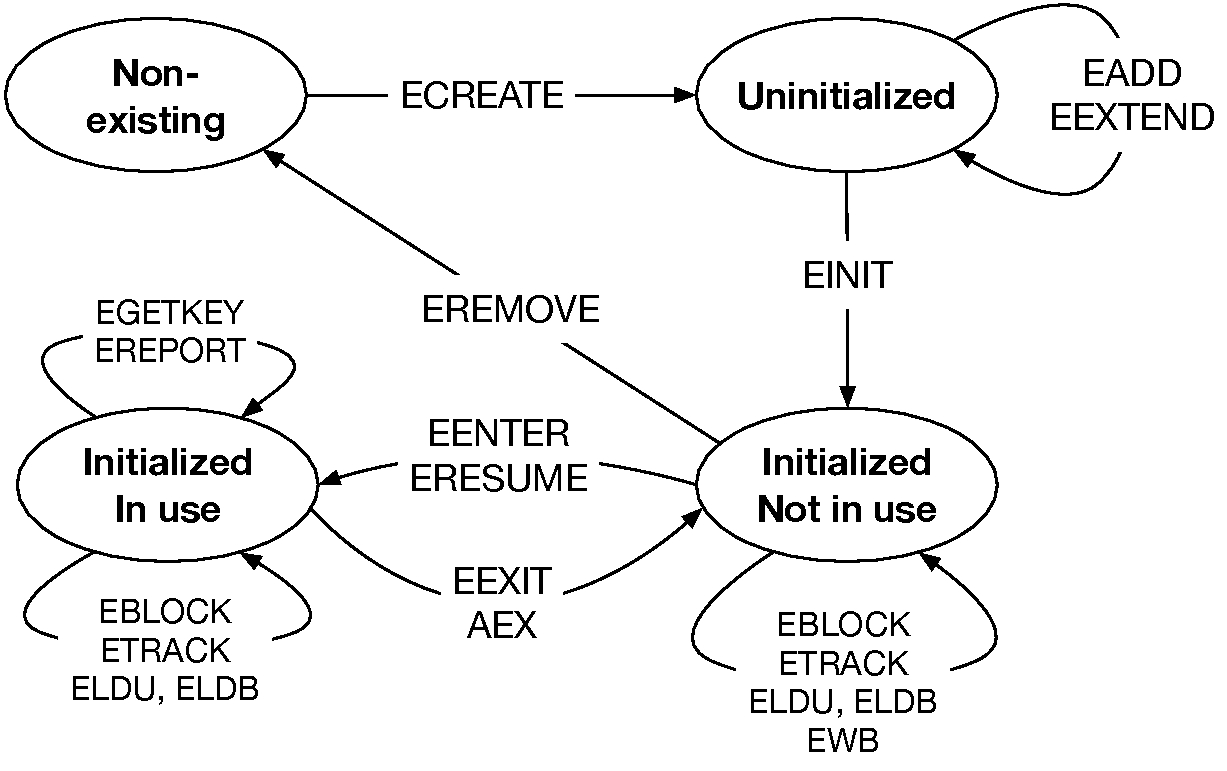
\includegraphics[width=85mm]{figures/sgx_enclave_lifecycle.pdf}
  \caption{
    The SGX enclave life cycle management instructions and state transition
    diagram
  }
  \label{fig:sgx_enclave_lifecycle}
\end{figure}


% Enclave Entry and Exiting : SDM S 39.2, S 39.2.1
% ECREATE, EADD, EREMOVE: SDM S 41.3

\subsubsection{Creation}
\label{sec:sgx_ecreate}

An enclave is born when the system software issues the \texttt{ECREATE}
instruction, which turns a free EPC page into the SECS~(\S~\ref{sec:sgx_secs})
for the new enclave.

\texttt{ECREATE} initializes the newly created SECS using the information in a
non-EPC page owned by the system software. This page specifies the values for
all the SECS fields defined in the SDM, such as BASEADDR and SIZE, using an
architectural layout that is guaranteed to be preserved by future
implementations.

While is very likely that the actual SECS layout used by initial SGX
implementations matches the architectural layout quite closely, future
implementations are free to deviate from this layout, as long as they maintain
the ability to initialize the SECS using the architectural layout.
Software cannot access an EPC page that holds a SECS, so it cannot become
dependent on an internal SECS layout. This is a stronger version of the
encapsulation used in the Virtual Machine Constrol
Structure~(VMCS,~\S~\ref{sec:vmx}).

\texttt{ECREATE} validates the information used to initialize the SECS, and
results in a page fault~(\#PF,~\S~\ref{sec:faults}) or general protection
fault~(\#GP,~\S~\ref{sec:faults}) if the information is not valid. For example,
if the SIZE field is not a power of two, \texttt{ECREATE} results in \#GP. This
validation, combined with the fact that the SECS is not accessible by software,
simplifies the implementation of the other SGX instructions, which can assume
that the information inside the SECS is valid.

Last, \texttt{ECREATE} initializes the enclave's INIT attribute (sub-field of
the ATTRIBUTES field in the enclave's SECS, \S~\ref{sec:sgx_secs_attributes})
to the false value. The enclave's code cannot be executed until the INIT
attribute is set to true, which happens in the initialization stage that will
be described in \S~\ref{sec:sgx_einit_overview}.


\subsubsection{Loading}
\label{sec:sgx_eadd}

\texttt{ECREATE} marks the newly created SECS as \textit{uninitialized}. While
an enclave's SECS is in this state, the system software can use \texttt{EADD}
instructions to load the initial code and data into the enclave. \texttt{EADD}
is used to create both TCS pages (\S~\ref{sec:sgx_tcs}) and regular pages.

% Page Information (PAGEINFO): SDM S 38.10
% Security Information (SECINFO): SDM S 38.11

\texttt{EADD} reads its input data from a \textit{Page Information}~(PAGEINFO)
structure, illustrated in Figure~\ref{fig:sgx_pageinfo}. The structure's
contents are only used to communicate information to the SGX implementation, so
it is entirely architectural and documented in the SDM.

\begin{figure}[hbt]
  \centering
  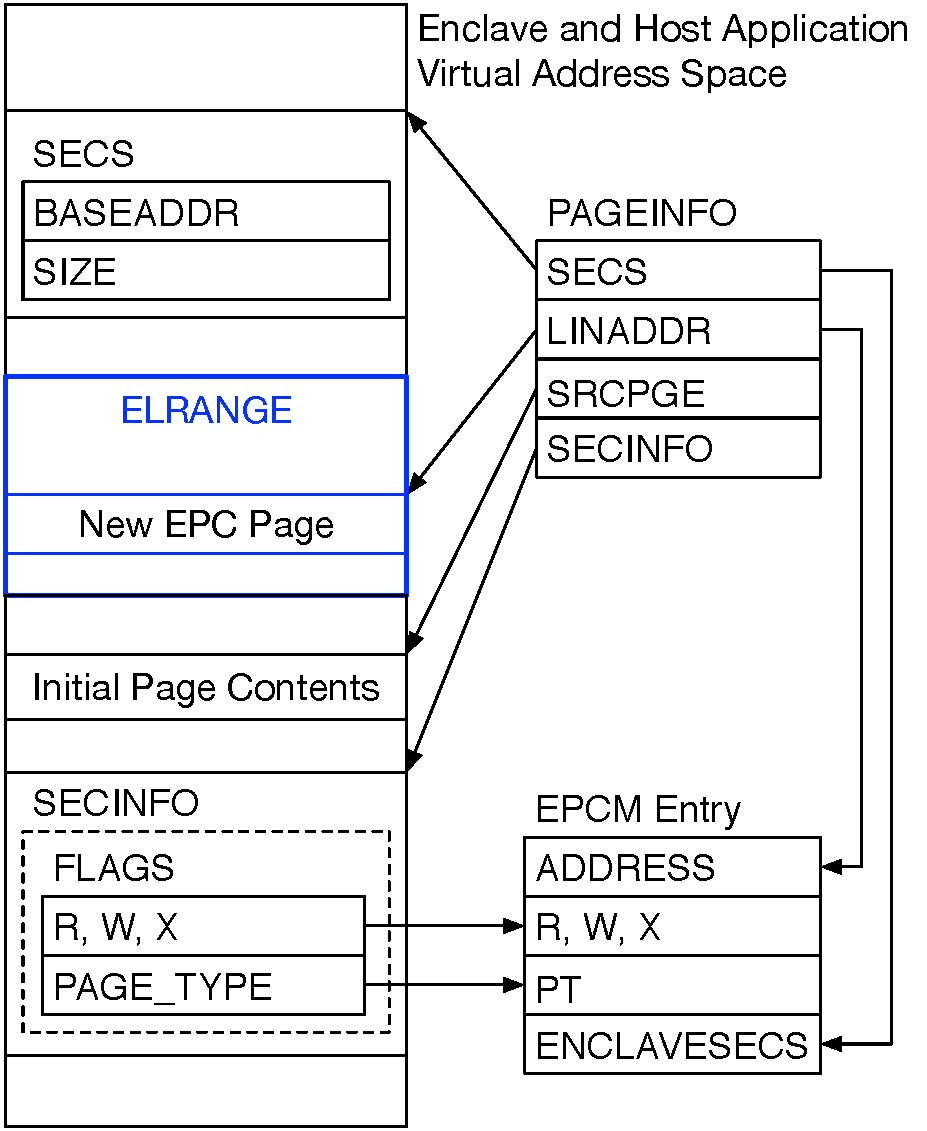
\includegraphics[width=65mm]{figures/sgx_pageinfo.pdf}
  \caption{
    The PAGEINFO structure supplies input data to SGX instructions such as
    \texttt{EADD}.
  }
  \label{fig:sgx_pageinfo}
\end{figure}

Currently, the PAGEINFO structure contains the virtual address of the EPC page
that will be allocated (LINADDR), the virtual address of the non-EPC page whose
contents will be copied into the newly allocated EPC page (SRCPGE), a virtual
address that resolves to the SECS of the enclave that will own the page (SECS),
and values for some of the fields of the EPCM entry associated with the newly
allocated EPC page (SECINFO).

The SECINFO field in the PAGEINFO structure is actually a virtual memory
address, and points to a \textit{Security Information}~(SECINFO) structure,
some of which is also illustrated in Figure~\ref{fig:sgx_pageinfo}. The SECINFO
structure contains the newly allocated EPC page's access permissions (R, W, X)
and its EPCM page type (PT\_REG or PT\_TCS). Like PAGEINFO, the SECINFO
structure is solely used to communicate data to the SGX implementation, so its
contents are also entirely architectural. However, most of the structure's
64 bytes are reserved for future use.

Both the PAGEINFO and the SECINFO structures are prepared by the system
software that invokes the \texttt{EADD} instruction, and therefore must be
contained in non-EPC pages. Both structures must be aligned to their sizes --
PAGEINFO is 32 bytes long, so each PAGEINFO instance must be 32-byte aligned,
while SECINFO has 64 bytes, and therefore each SECINFO instance must be
64-byte aligned. The alignment requirements likely simplify the SGX
implementation by reducing the number of special cases that must be handled.

\texttt{EADD} validates its inputs before modifying the newly allocated EPC
page or its EPCM entry. Most importantly, attempting to \texttt{EADD} a page to
an enclave whose SECS is in the initialized state will result in a \#GP.
Furthermore, attempting to \texttt{EADD} an EPC page that is already allocated
(the VALID field in its EPCM entry is 1) results in a \#PF. \texttt{EADD} also
ensures that the page's virtual address falls within the enclave's ELRANGE, and
that all the reserved fields in SECINFO are set to zero.

While loading an enclave, the system software will also use the
\texttt{EEXTEND} instruction, which updates the enclave's measurement used in
the software attestation process. Software attestation is discussed in
\S~\ref{sec:sgx_attestation}.


\subsubsection{Initialization}
\label{sec:sgx_einit_overview}

% EINIT Token Structure (EINITTOKEN): SDM S 38.14

After loading the initial code and data pages into the enclave, the system
software must use a \textit{Launch Enclave}~(LE) to obtain an EINIT Token
Structure, via an under-documented process that will be described in more
detail in \S~\ref{sec:sgx_launch_enclave}. The token is then provided to the
\texttt{EINIT} instruction, which marks the enclave's SECS as
\textit{initialized}.

The LE is a privileged enclave provided by Intel, and \textbf{is a prerequisite
for the use of enclaves authored by parties other than Intel}. The LE is an
SGX enclave, so it must be created, loaded and initialized using the processes
described in this section. However, the LE is cryptographically
signed~(\S~\ref{sec:integrity_crypto}) with a special Intel key that is
hard-coded into the SGX implementation, and that causes \texttt{EINIT} to
initialize the LE  without checking for a valid EINIT Token Structure.

When \texttt{EINIT} completes successfully, it sets the enclave's INIT
attribute to true. This opens the way for ring 3~(\S~\ref{sec:rings})
application software to execute the enclave's code, using the SGX instructions
described in \S~\ref{sec:sgx_threads}. On the other hand, once INIT is set to
true, \texttt{EADD} cannot be invoked on that enclave anymore, so the system
software must load all the pages that make up the enclave's initial state
before executing the \texttt{EINIT} instruction.


\subsubsection{Teardown}
\label{sec:sgx_eremove}

After the enclave has done the computation it was designed to perform, the
system software executes the \texttt{EREMOVE} instruction to deallocate the
EPC pages used by the enclave.

\texttt{EREMOVE} marks an EPC page as available by setting the VALID field of
the page's EPCM entry to 0 (zero). Before freeing up the page, \texttt{EREMOVE}
makes sure that there is no logical processor executing code inside the enclave
that owns the page to be removed.

An enclave is completely destroyed when the EPC page holding its SECS is freed.
\texttt{EREMOVE} refuses to deallocate a SECS page if it is referenced by any
other EPCM entry's ENCLAVESECS field, so an enclave's SECS page can only be
deallocated after all the enclave's pages have been deallocated.

\HeadingLevelB{The Life Cycle of an SGX Thread}
\label{sec:sgx_threads}

Between the time when an enclave is
initialized~(\S~\ref{sec:sgx_einit_overview}) and the time when it is torn
down~(\S~\ref{sec:sgx_eremove}), the enclave's code can be executed by any
application process that has the enclave's EPC pages mapped into its virtual
address space.

% Internal CREGs: SDM S 41.1.4
% Access Control Requirements: SDM S 38.3

When executing the code inside an enclave, a logical processor is said to be
\textit{in enclave mode}, and the code that it executes can access the
regular~(PT\_REG,~\S~\ref{sec:sgx_epcm}) EPC pages that belong to the currently
executing enclave. When a logical process is outside enclave mode, it bounces
any memory accesses inside the Processor Reserved Memory
range~(PRM,~\S~\ref{sec:sgx_prm}), which includes the EPC.

Each logical processor that executes enclave code uses a Thread Control
Structure~(TCS,~\S~\ref{sec:sgx_tcs}). When a TCS is used by a logical
processor, it is said to be \textit{busy}, and it cannot be used by any other
logical processor.  Figure~\ref{fig:sgx_tcs_lifecycle} illustrates the
instructions used by a host process to execute enclave code and their
interactions with the TCS that they target.

\begin{figure}[hbt]
  \centering
  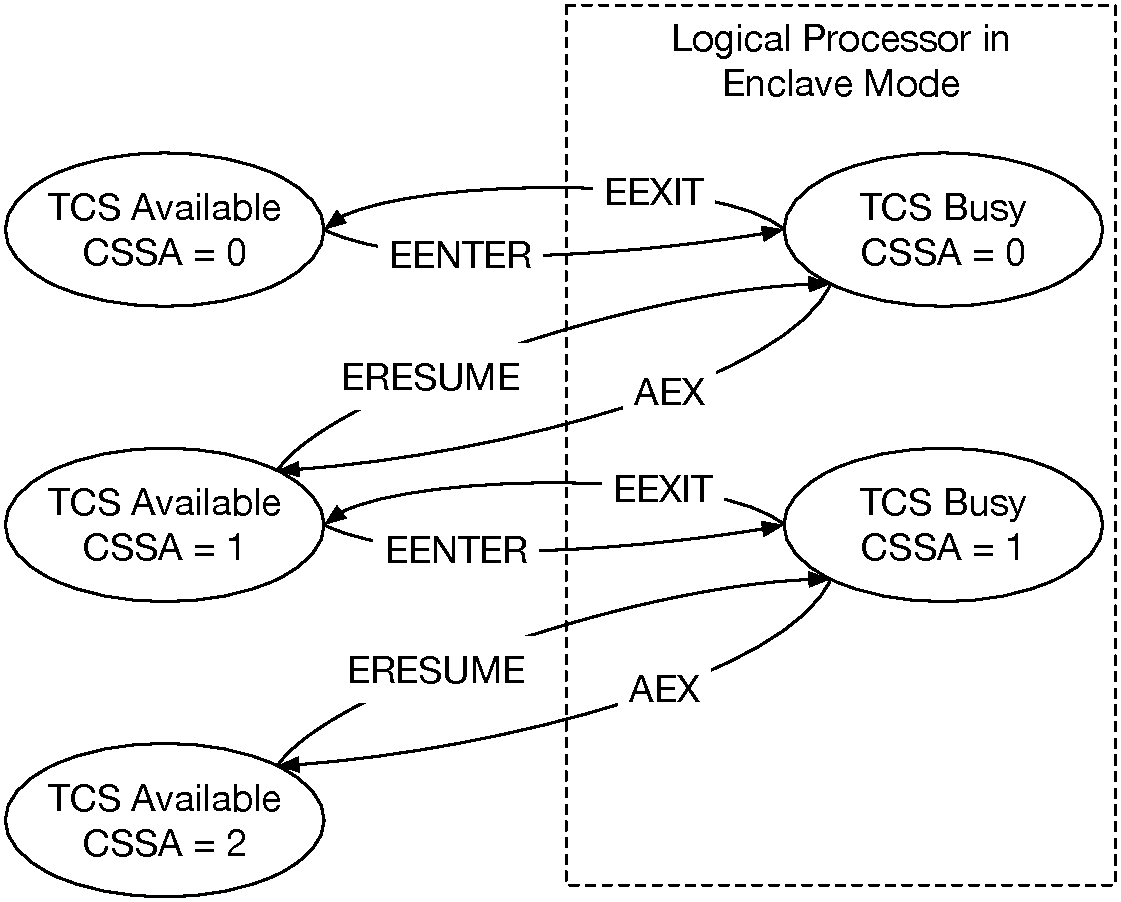
\includegraphics[width=75mm]{figures/sgx_tcs_lifecycle.pdf}
  \caption{
    The stages of the life cycle of an SGX Thread Control Structure (TCS) that
    has two State Save Areas (SSAs).
  }
  \label{fig:sgx_tcs_lifecycle}
\end{figure}

Assuming that no hardware exception occurs, an enclave's host process uses the
\texttt{EENTER} instruction, described in \S~\ref{sec:sgx_eenter}, to execute
enclave code. When the enclave code finishes performing its task, it uses the
\texttt{EEXIT} instruction, covered in \S~\ref{sec:sgx_eexit}, to return the
execution control to the host process that invoked the enclave.

If a hardware exception occurs while a logical processor is in enclave mode,
the processor is taken out of enclave mode using an
\textit{Asynchronous Enclave Exit}~(AEX), summarized in \S~\ref{sec:sgx_aex},
before the system software's exception handler is invoked. After the system
software's handler is invoked, the enclave's host process can use the
\texttt{ERESUME} instruction, described in \S~\ref{sec:sgx_eresume}, to
re-enter the enclave and resume the computation that it was performing.


\HeadingLevelC{Synchronous Enclave Entry}
\label{sec:sgx_enclave_mode}
\label{sec:sgx_eenter}

At a high level, \texttt{EENTER} performs a controlled jump into enclave code,
while performing the processor configuration that is needed by SGX's security
guarantees. Going through all the configuration steps is a tedious exercise,
but it a necessary prerequisite to understanding how all data structures used
by SGX work together. For this reason, \texttt{EENTER} and its siblings are
described in much more detail than the other SGX instructions.

% ENCLU - Execute an Enclave User Function of Specified Leaf Number: SDM S 41.2

\texttt{EENTER}, illustrated in Figure~\ref{fig:sgx_eenter} can only be
executed by unprivileged application software running at ring
3~(\S~\ref{sec:rings}), and results in an undefined instruction (\#UD) fault if
is executed by system software.

\begin{figure}[hbt]
  \centering
  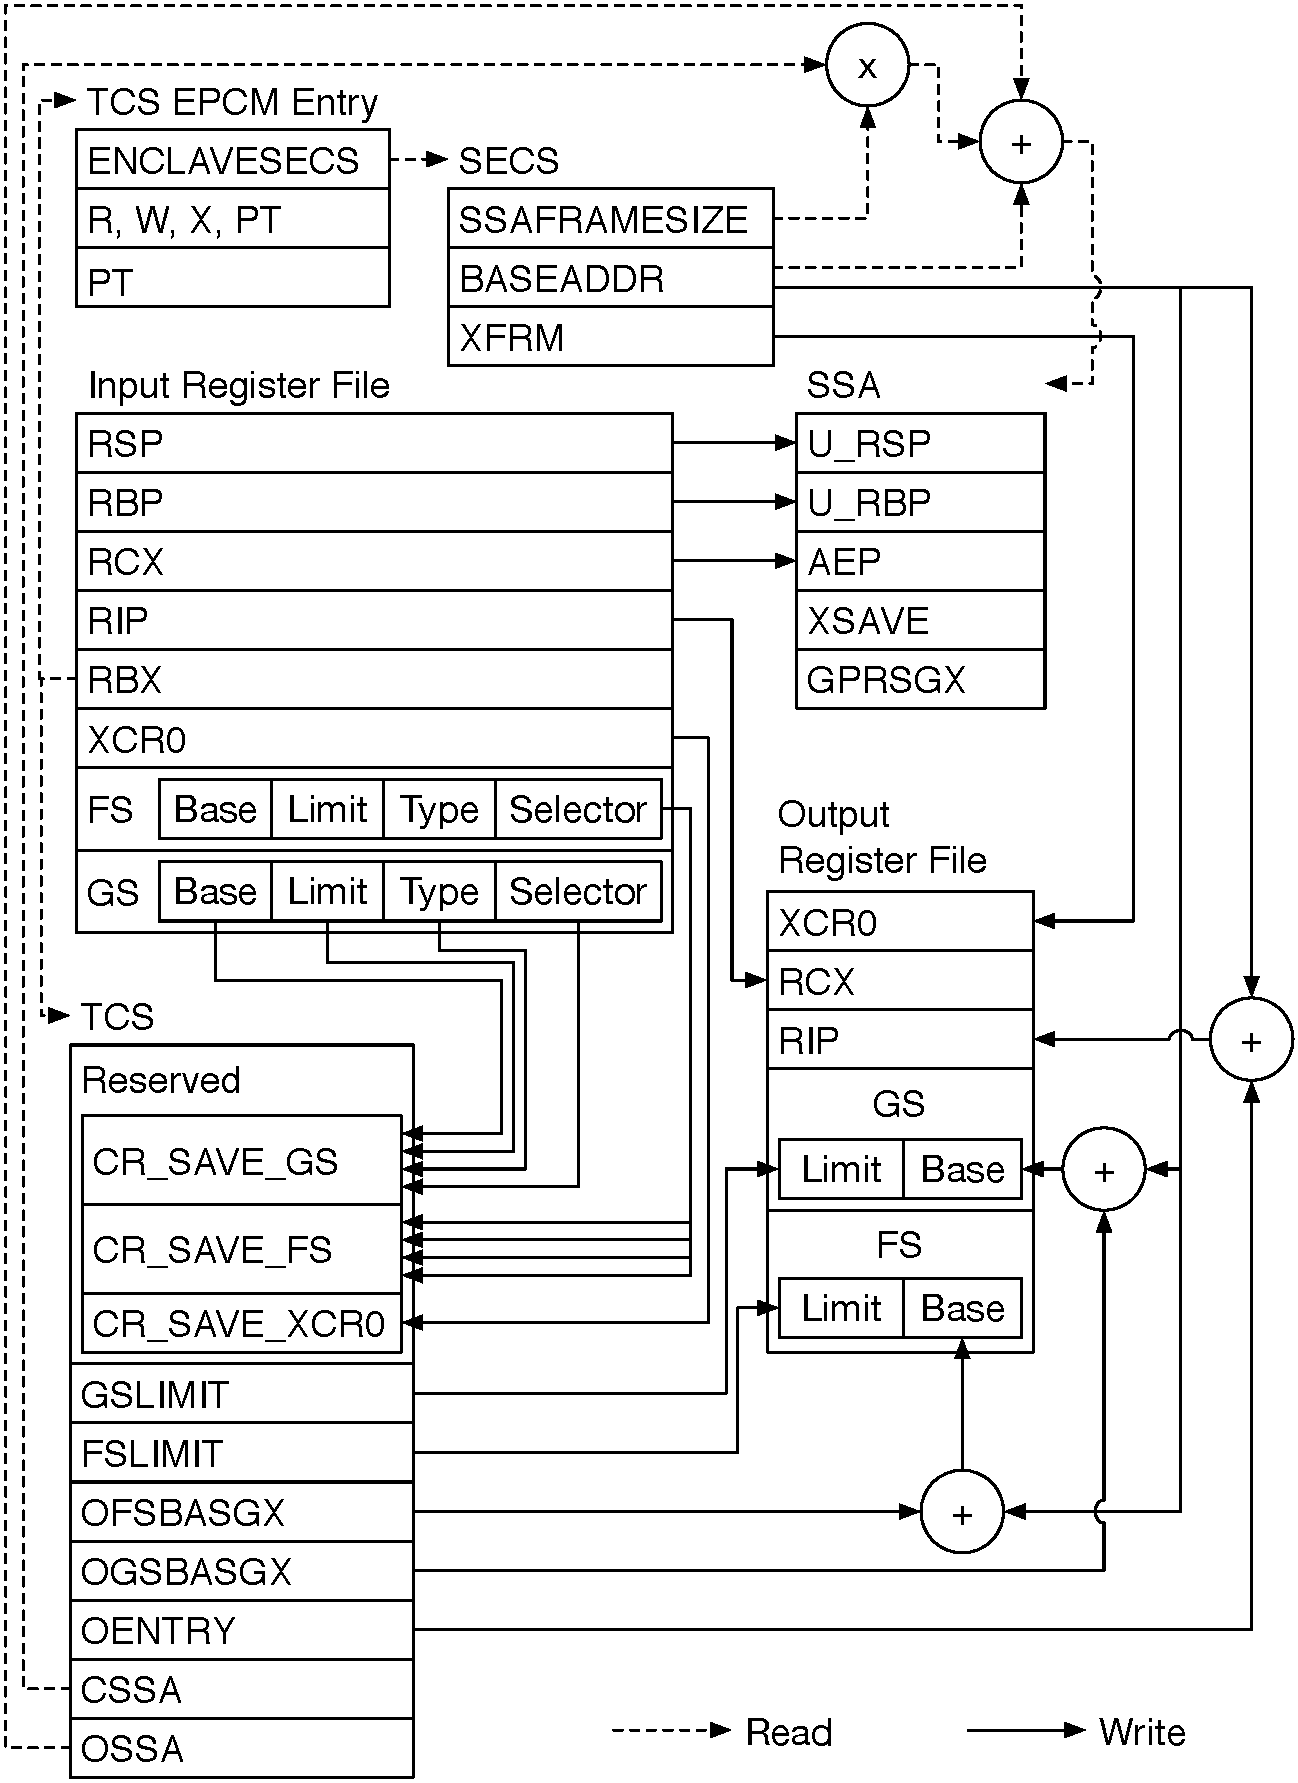
\includegraphics[width=87mm]{figures/sgx_eenter.pdf}
  \caption{
    Data flow diagram for a subset of the logic in \texttt{EENTER}. The figure
    omits the logic for disabling debugging features, such as hardware
    breakpoints and performance monitoring events.
  }
  \label{fig:sgx_eenter}
\end{figure}

\texttt{EENTER} switches the logical processor to enclave mode, but does not
perform a privilege level switch~(\S~\ref{sec:faults}). Therefore, enclave code
always executes at ring 3, with the same privileges as the application code
that calls it. This makes it possible for an infrastructure owner to allow
user-supplied software to create and use enclaves, while having the assurance
that the OS kernel and hypervisor can still protect the infrastructure from
buggy or malicious software.

% EENTER - Enters an Enclave: SDM S 41.4.1
% Current State Save Area Frame (CSSA): SDM S 38.8.3
% Number of State Save Area Frames (NSSA): SDM S 38.8.4

\texttt{EENTER} takes the virtual address of a TCS as its input, and requires
that the TCS is \textit{available} (not busy), and that at least one State Save
Area~(SSA,~\S~\ref{sec:sgx_ssa}) is available in the TCS. The latter check is
implemented by making sure that the \textit{current SSA index}~(CSSA) field in
the TCS is less than the number of SSAs (NSSA) field. The SSA indicated by the
CSSA, which shall be called the \textit{current SSA}, is used in the event that
a hardware exception occurs while enclave code is executed.

\texttt{EENTER} transitions the logical processor into enclave mode, and sets
the instruction pointer (RIP) to the value indicated by the \textit{entry point
offset}~(OENTRY) field in the TCS that it receives. \textit{EENTER} is used by
an untrusted caller to execute code in a protected environment, and therefore
has the same security considerations as
\texttt{SYSCALL}~(\S~\ref{sec:privilege_switches}), which is used to call into
system software. Setting RIP to the value indicated by OENTRY guarantees to the
enclave author that the enclave code will only be invoked at well defined
points, and prevents a malicious host application from bypassing any security
checks that the enclave author may perform.

% Interactions with the Processor Extended State and Misc State: SDM S 42.7
% SECS.ATTRIBUTES.XFRM: SDM S 42.7.2.1

\texttt{EENTER} also sets XCR0~(\S~\ref{sec:registers}), the register that
controls which extended architectural features are in use, to the value of the
XFRM enclave attribute~(\S~\ref{sec:sgx_secs_attributes}). Ensuring that XCR0 is
set according to the enclave author's intentions prevents a malicious operating
system from bypassing an enclave's security by enabling architectural features
that the enclave is not prepared to handle.

Furthermore, \texttt{EENTER} loads the bases of the segment
registers~(\S~\ref{sec:segments}) FS and GS using values specified in the TCS.
The segments' selectors and types are hard-coded to safe values for ring 3 data
segments. This aspect of the SGX design makes it easy to implement per-thread
Thread Local Storage (TLS). For 64-bit enclaves, this is a convenience feature
rather than a security measure, as enclave code can securely load new bases
into FS and GS using the \texttt{WRFSBASE} and \texttt{WRGSBASE} instructions.

The \texttt{EENTER} implementation backs up the old values of the registers
that it modifies, so they can be restored when the enclave finishes its
computation. Just like \texttt{SYSCALL}, \texttt{EEENTER} saves the address of
the following instruction in the RCX register.

Interestingly, the SDM states that the old values of the XCR0, FS, and GS
registers are saved in new registers dedicated to the SGX implementation.
However, given that they will only be used on an enclave exit, we expect that
the registers are saved in DRAM, in the reserved area in the TCS.

Like \texttt{SYSCALL}, \texttt{EENTER} does not modify the stack pointer
register (RSP). To avoid any security exploits, enclave code should set RSP to
point to a stack area that is entirely contained in EPC pages. Multi-threaded
enclaves can easily implement per-thread stack areas by setting up each
thread's TLS area to include a pointer to the thread's stack, and by setting
RSP to the value obtained by reading the TLS area at which the FS or GS segment
points.

Last, when \texttt{EENTER} enters enclave mode, it suspends some of the
processor's debugging features, such as hardware breakpoints and Precise Event
Based Sampling~(PEBS). Conceptually, a debugger attached to the host process
sees the enclave's execution as one single processor instruction.


\HeadingLevelC{Synchronous Enclave Exit}
\label{sec:sgx_eexit}

% EEXIT - Exits an Enclave: SDM S 41.4.1

\texttt{EEXIT} can only be executed while the logical processor is in enclave
mode, and results in a (\#UD) if executed in any other circumstances. In a
nutshell, the instruction returns the processor to ring 3 outside enclave mode
and restores the registers saved by \texttt{EENTER}, which were described above.

Unlike \texttt{SYSRET}, \texttt{EEXIT} sets RIP to the value read from RBX,
after exiting enclave mode. This is inconsistent with \texttt{EENTER}, which
saves the RIP value to RCX. Unless this inconsistency stems from an error in
the SDM, enclave code must be sure to note the difference.

The SDM explicitly states that \texttt{EEXIT} does not modify most registers,
so enclave authors must make sure to clear any secrets stored in the
processor's registers before returning control to the host process.
Furthermore, enclave software will most likely cause a fault in its caller if
it doesn't restore the stack pointer RSP and the stack frame base pointer RBP
to the values that they had when \texttt{EENTER} was called.

It may seem unfortunate that enclave code can induce faults in its caller.
For better or for worse, this perfectly matches the case where an application
calls into a dynamically loaded module. More specifically, the module's code is
also responsible for preserving stack-related registers, and a buggy module
might jump anywhere in the application code of the host process.

This section describes the \texttt{EENTER} behavior for 64-bit enclaves. The
\texttt{EENTER} implementation for 32-bit enclaves is significantly more
complex, due to the extra special cases introduced by the full-fledged
segmentation model that is still present in the 32-bit Intel architecture. As
stated in the introduction, we are not interested in such legacy aspects.


\HeadingLevelC{Asynchronous Enclave Exit (AEX)}
\label{sec:sgx_aex}

If a hardware exception, like a fault~(\S~\ref{sec:faults}) or an
interrupt~(\S~\ref{sec:interrupts}), occurs while a logical processor is
executing an enclave's code, the processor performs an
\textit{Asynchronous Enclave Exit}~(AEX) before invoking the system software's
exception handler, as shown in Figure~\ref{fig:sgx_aex_setup}.

\begin{figure}[hbt]
  \centering
  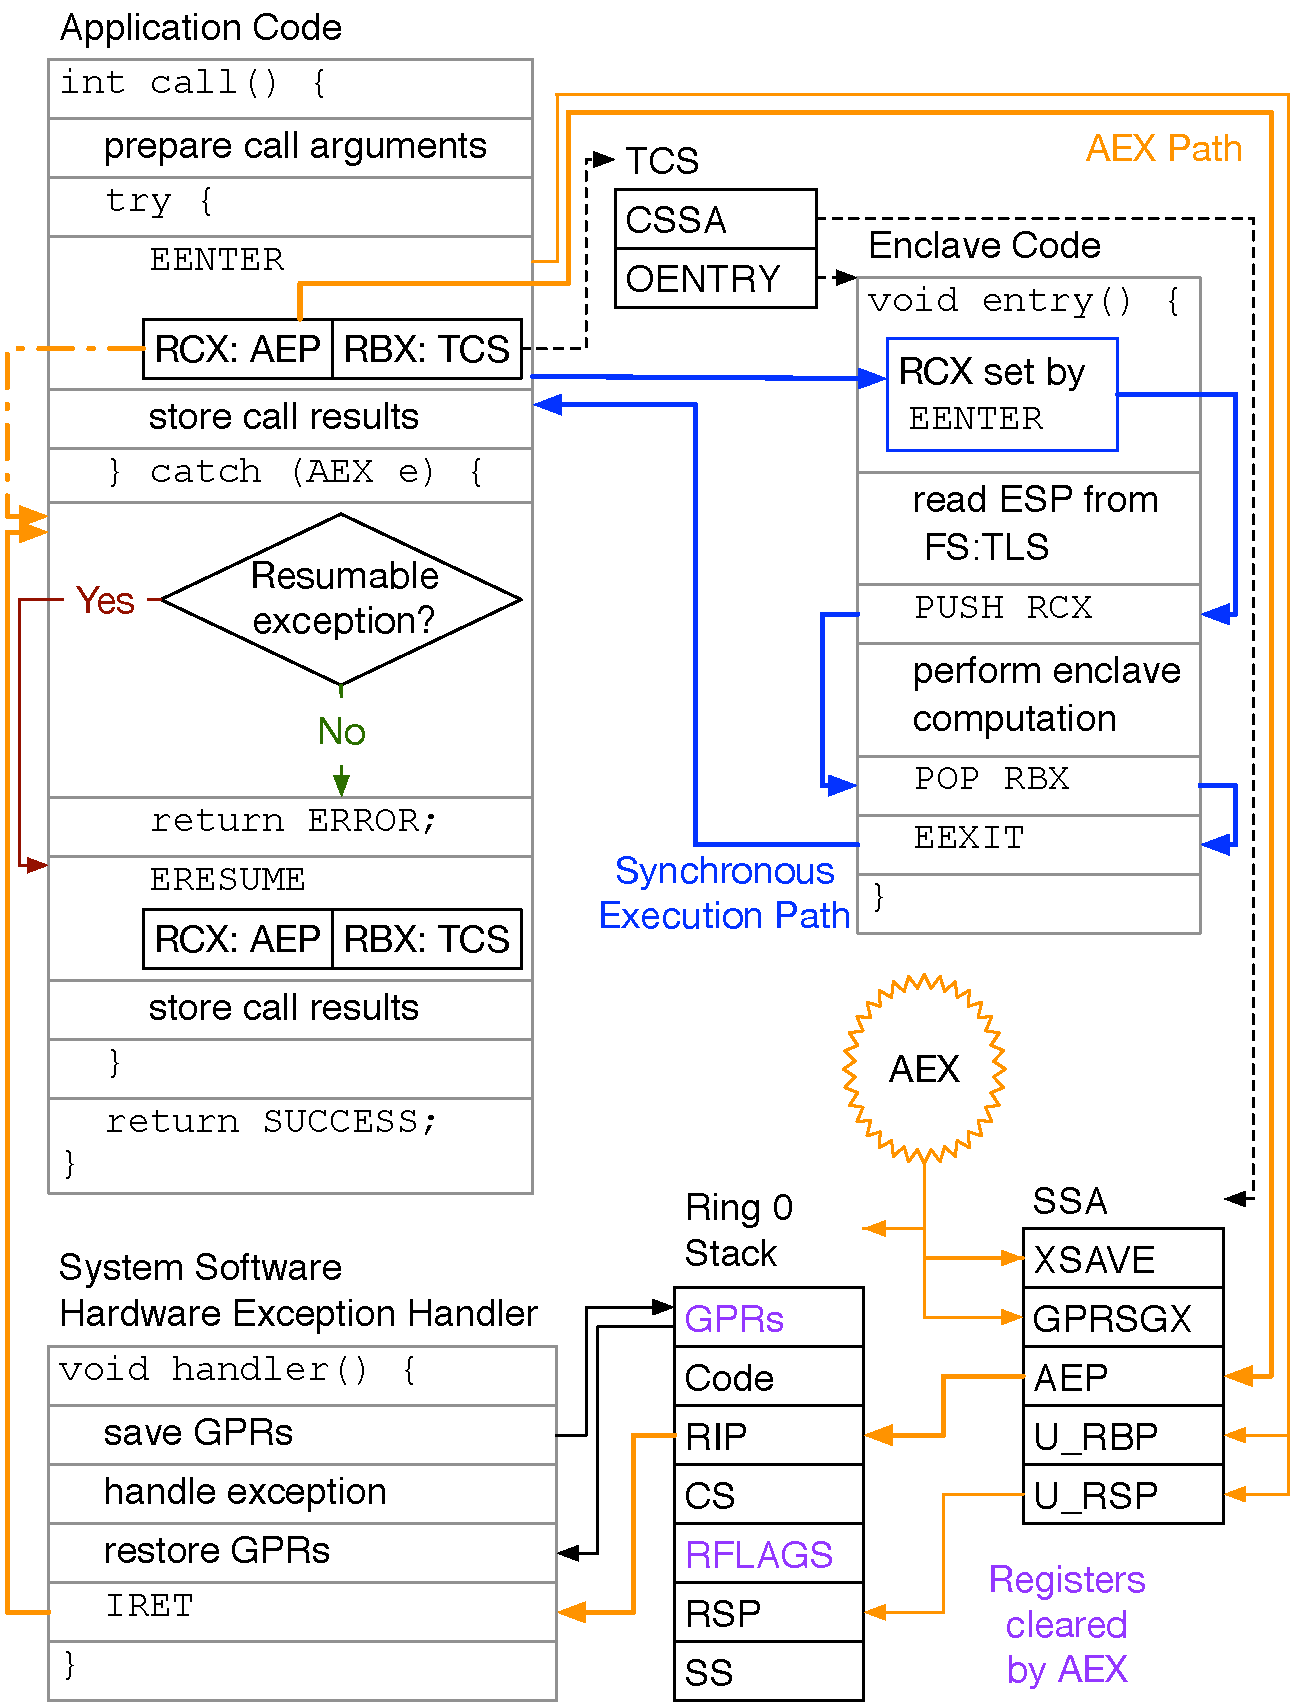
\includegraphics[width=87mm]{figures/sgx_aex_setup.pdf}
  \caption{
    If a hardware exception occurs during enclave execution, the synchronous
    execution path is aborted, and an Asynchronous Enclave Exit (AEX) occurs
    instead.
  }
  \label{fig:sgx_aex_setup}
\end{figure}

% AEX Flow: SDM S 40.4
% AEX Operational Detail: SDM S 40.4.1

The AEX saves the enclave code's execution context~(\S~\ref{sec:registers}),
restores the state saved by \texttt{EENTER}, and sets up the processor
registers so that the system software's hardware exception handler will return
to an \textit{asynchronous exit handler} in the enclave's host process. The
exit handler is expected to use the \texttt{ERESUME} instruction to resume the
enclave computation that was interrupted by the hardware exception.

Asides from the behavior described in \S~\ref{sec:sgx_eenter}, \texttt{EENTER}
also writes some information to the current SSA, which is only used if an AEX
occurs. As shown in Figure~\ref{fig:sgx_eenter}, \texttt{EENTER} stores the
stack pointer register RSP and the stack frame base pointer register RBP into
the U\_RSP and U\_RBP fields in the current SSA. Last, \texttt{EENTER} stores
the value in RCX in the \textit{Asynchronous Exit handler Pointer}~(AEP) field
in the current SSA.

When a hardware exception occurs in enclave mode, the SGX implementation
performs a sequence of steps that takes the logical processor out of enclave
mode and invokes the hardware exception handler in the system software.
Conceptually, the SGX implementation first performs an AEX to take the logical
processor out of enclave mode, and then the hardware exception is handled
using the standard Intel architecture's behavior described in
\S~\ref{sec:faults}. Actual Intel processors may interleave the AEX
implementation with the exception handling implementation. However, for
simplicity, this work describes AEX as a separate process that is performed
before any exception handling steps are taken.

In the Intel architecture, if a hardware exception occurs, the application
code's execution context can be read and modified by the system software's
exception handler (\S~\ref{sec:faults}). This is acceptable when the system
software is trusted by the application software. However, under SGX's threat
model, the system software is not trusted by enclaves. Therefore, the AEX step
erases any secrets that may exist in the execution state by resetting all its
registers to predefined values.

% State Saving by AEX: SDM S 40.2

Before the enclave's execution state is reset, it is backed up inside the
current SSA. Specifically, an AEX backs up the general purpose
registers~(GPRs,~\S~\ref{sec:registers}) in the GPRSGX area in the SSA, and
then performs an \texttt{XSAVE}~(\S~\ref{sec:registers}) using the
requested-feature bitmap (RFBM) specified in the XFRM field in the enclave's
SECS. As each SSA is entirely stored in EPC pages allocated to the enclave, the
system software cannot read or tamper with the backed up execution state. When
an SSA receives the enclave's execution state, it is marked as used by
incrementing the CSSA field in the current TCS.

% Compatible Switch to the Exiting Stack of AEX: SDM S 40.1

After clearing the execution context, the AEX process sets RSP and RBP to the
values saved by \texttt{EENTER} in the current SSA, and sets RIP to the value
in the current SSA's AEP field. This way, when the system software's hardware
exception handler completes, the processor will execute the asynchronous exit
handler code in the enclave's host process. The SGX design makes it easy to
set up the asynchronous handler code as an exception handler in the routine
that contains the \texttt{EENTER} instruction, because the RSP and RBP
registers will have the same values as they had when \texttt{EENTER} was
executed.

Many of the actions taken by AEX to get the logical processor outside of
enclave mode match \texttt{EEXIT}. The segment registers FS and GS are restored
to the values saved by \texttt{EENTER}, and all the debugging facilities that
were suppressed by \texttt{EENTER} are restored to their previous states.


\HeadingLevelC{Recovering from an Asynchronous Exit}
\label{sec:sgx_eresume}

When a hardware exception occurs inside enclave mode, the processor performs
an AEX before invoking the exception's handler set up by the system software.
The AEX sets up the execution context in such a way that when the system
software finishes processing the exception, it returns into an asynchronous
exit handler in the enclave's host process. The asynchronous exception handler
usually executes the \texttt{ERESUME} instruction, which causes the logical
processor to go back into enclave mode and continue the computation that was
interrupted by the hardware exception.

\texttt{ERESUME} shares much of its functionality with \texttt{EENTER}. This is
best illustrated by the similarity between Figures
\ref{fig:sgx_aex_eresume} and \ref{fig:sgx_aex_setup}.

\begin{figure}[hbt]
  \centering
  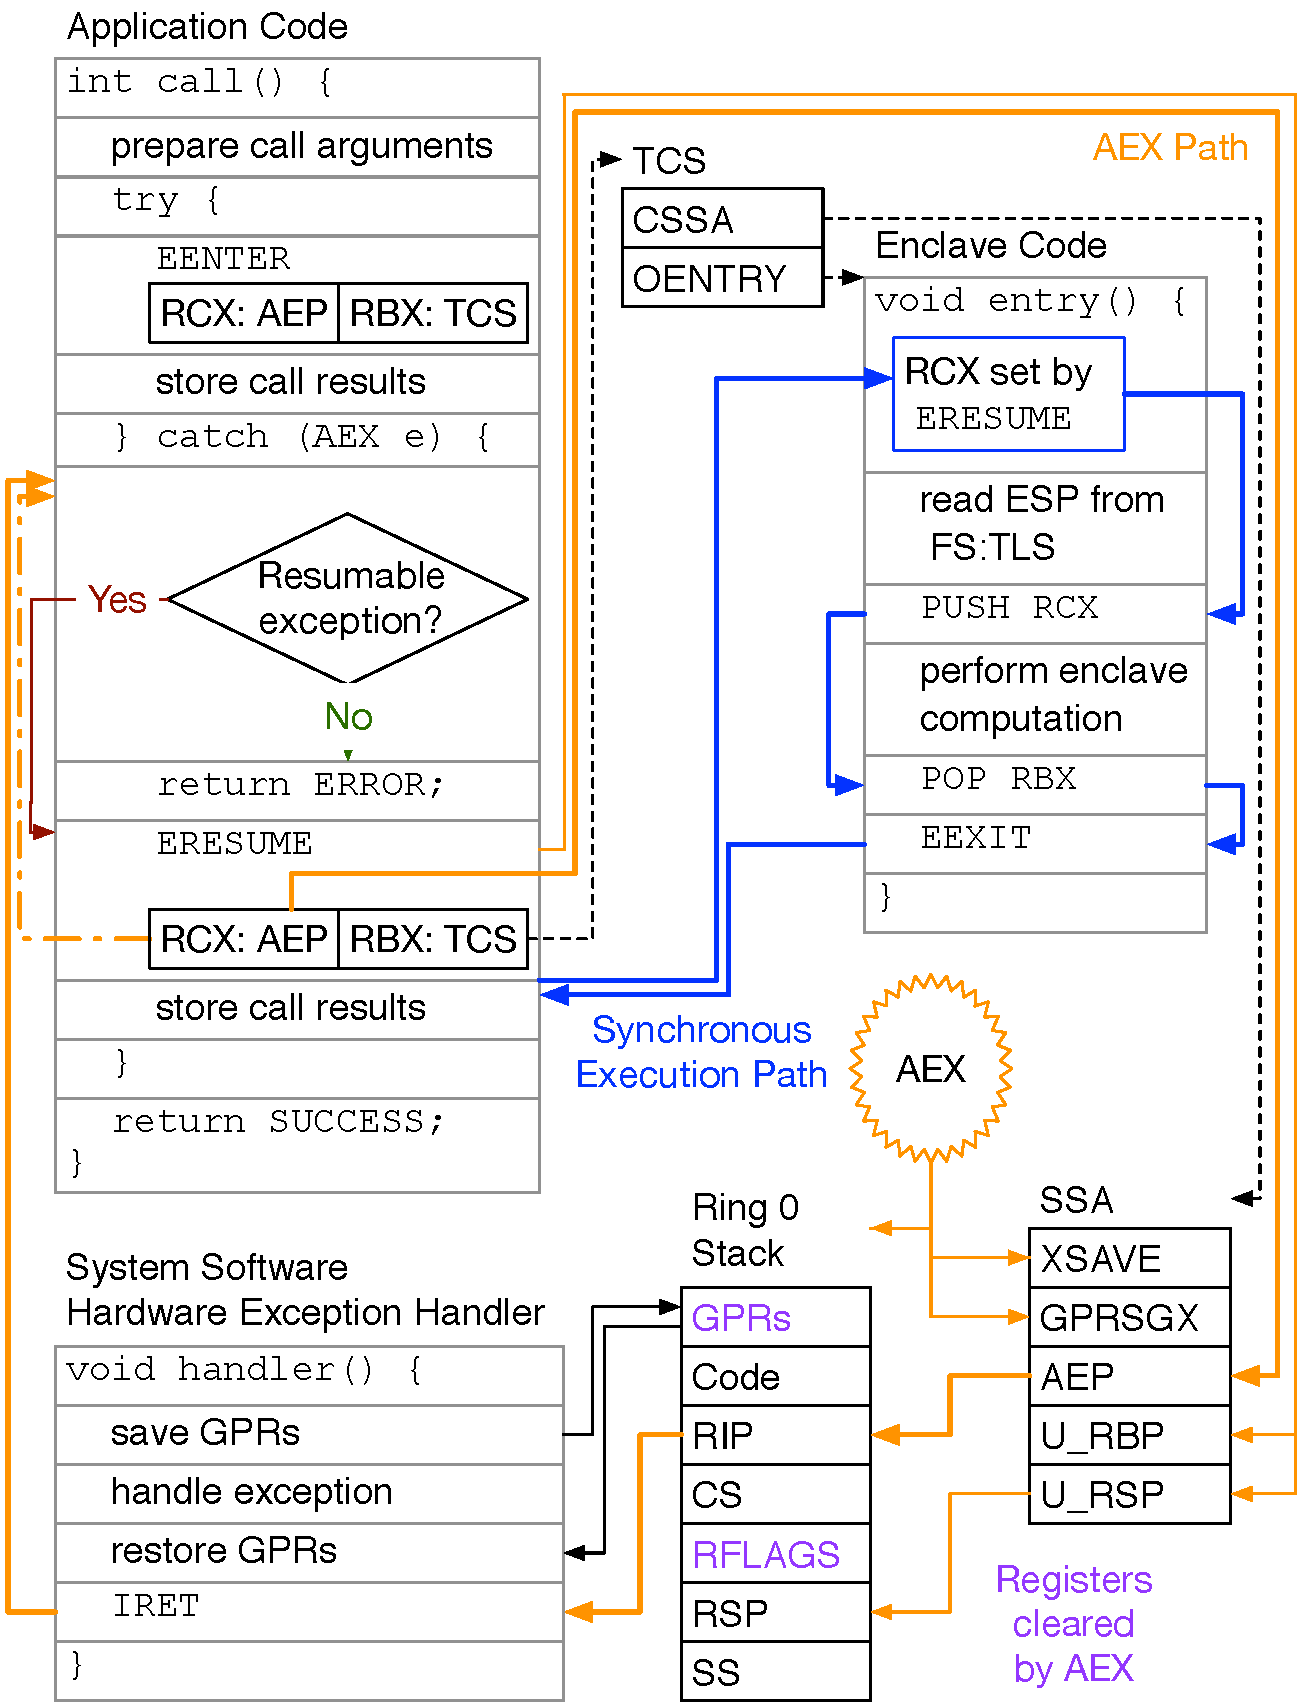
\includegraphics[width=87mm]{figures/sgx_aex_eresume.pdf}
  \caption{
    If a hardware exception occurs during enclave execution, the synchronous
    execution path is aborted, and an Asynchronous Enclave Exit (AEX) occurs
    instead.
  }
  \label{fig:sgx_aex_eresume}
\end{figure}

\texttt{EENTER} and \texttt{ERESUME} receive the same inputs, namely a pointer
to a TCS, described in \S~\ref{sec:sgx_eenter}, and an AEP, described in
\S~\ref{sec:sgx_aex}. The most common application design will pair each
\texttt{EENTER} instance with an asynchronous exit handler that invokes
\texttt{ERESUME} with exactly the same arguments.

The main difference between \texttt{ERESUME} and \texttt{EENTER} is that the
former uses an SSA that was ``filled out'' by an AEX~(\S~\ref{sec:sgx_aex}),
whereas the latter uses an empty SSA. Therefore, \texttt{ERESUME} results in a
\#GP fault if the CSSA field in the provided TCS is 0 (zero), whereas
\texttt{EENTER} fails if CSSA is greater than or equal to NSSA.

When successful, \texttt{ERESUME} decrements the CSSA field of the TCS, and
restores the execution context backed up in the SSA pointed to by the CSSA field
in the TCS. Specifically, the \texttt{ERESUME} implementation restores the
GPRs~(\S~\ref{sec:registers}) from the GPRSGX field in the SSA, and performs an
\texttt{XRSTOR}~(\S~\ref{sec:registers}) to load the execution state
associated with the extended architectural features used by the enclave.

\texttt{ERESUME} shares the following behavior with
\texttt{EENTER}~(\S~\ref{sec:sgx_eenter}). Both instructions write the U\_RSP,
U\_RBP, and AEP fields in the current SSA. Both instructions follow the same
process for backing up XCR0 and the FS and GS segment registers, and set them
to the same values, based on the current TCS and its enclave's SECS. Last, both
instructions disable the same subset of the logical processor's debugging
features.

An interesting edge case that \texttt{ERESUME} handles correctly is that it
sets XCR0 to the XFRM enclave attribute \textbf{before} performing an
\texttt{XRSTOR}. It follows that \texttt{ERESUME} fails if the requested
feature bitmap (RFBM) in the SSA is not a subset of XFRM. This matters because,
while an AEX will always use the XFRM value as the RFBM, enclave code executing
on another thread is free to modify the SSA contents before \texttt{ERESUME} is
called.

The correct sequencing of actions in the \texttt{ERESUME} implementation
prevents a malicious application from using an enclave to modify registers
associated with extended architectural features that are not declared in XFRM.
This would break the system software's ability to provide thread-level
execution context isolation.

\HeadingLevelB{EPC Page Eviction}
\label{sec:sgx_epc_eviction}

Modern OS kernels take advantage of address translation~(\S~\ref{sec:paging})
to implement page swapping, also referred to as paging~(\S~\ref{sec:paging}).
In a nutshell, paging allows the OS kernel to over-commit the computer's DRAM
by evicting rarely used memory pages to a slower storage medium called the disk.

Paging is a key contributor to utilizing a computer's resources effectively.
For example, a desktop system whose user runs multiple programs concurrently
can evict memory pages allocated to inactive applications without a significant
degradation in user experience.

Unfortunately, the OS cannot be allowed to evict an enclave's EPC pages via the
same methods that are used to implement page swapping for DRAM memory outside
the PRM range. In the SGX threat model, enclaves do not trust the system
software, so the SGX design offers an EPC page eviction method that can defend
against a malicious OS that attempts any of the active address translation
attacks described in \S~\ref{sec:address_translation_attacks}.

The price of the security afforded by SGX is that an OS kernel that supports
evicting EPC pages must use a modified page swapping implementation that
interacts with the SGX mechanisms. Enclave authors can mostly ignore EPC
evictions, similarly to how today's application developers can ignore the OS
kernel's paging implementation.

As illustrated in Figure~\ref{fig:sgx_page_eviction}, SGX supports evicting
EPC pages to DRAM pages outside the PRM range. The system software is expected
to use its existing page swapping implementation to evict the contents of these
pages out of DRAM and onto a disk.

\begin{figure}[hbt]
  \centering
  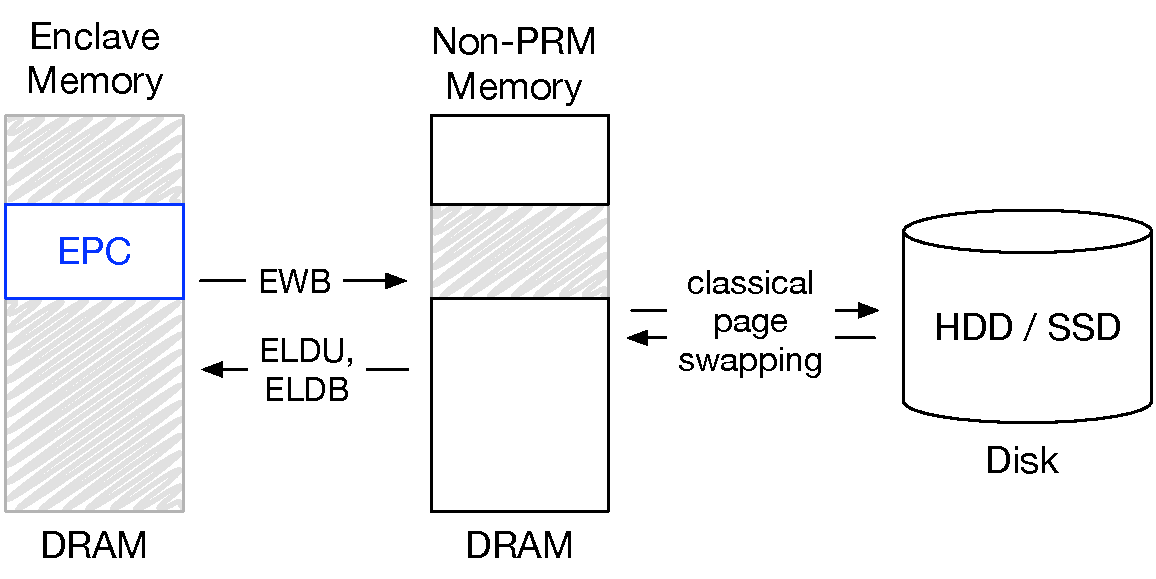
\includegraphics[width=85mm]{figures/sgx_page_eviction.pdf}
  \caption{
    SGX offers a method for the OS to evict EPC pages into non-PRM DRAM. The
    OS can then use its standard paging feature to evict the pages out of DRAM.
  }
  \label{fig:sgx_page_eviction}
\end{figure}

SGX's eviction feature revolves around the \texttt{EWB} instruction, described
in detail in \S~\ref{sec:sgx_ewb}. Essentially, \texttt{EWB} evicts an EPC page
into a DRAM page outside the EPC and marks the EPC page as available, by
zeroing the VALID field in the page's EPCM entry.

The SGX design relies on symmetric key cryptograpy~\ref{sec:crypto_keys} to
guarantee the privacy and integrity of the evicted EPC pages, and on
nonces~(\S~\ref{sec:freshness_crypto}) to guarantee the freshness of the pages
brought back into the EPC. These nonces are stored in Version Arrays~(VAs),
covered in \S~\ref{sec:sgx_va}, which are EPC pages dedicated to nonce storage.

Before an EPC page is evicted and freed up for use by other enclaves, the SGX
implementation must ensure that no TLB has address translations associated with
the evicted page, in order to avoid the TLB-based address translation attack
described in \S~\ref{sec:tlb_mapping_attacks}.

As explained in \S~\ref{sec:sgx_epc}, SGX leaves the system software in charge
of managing the EPC. It naturally follows that the SGX instructions described
in this section, which are used to implement EPC paging, are only available to
system software, which runs at ring 0~\S~\ref{sec:rings}.

In today's software stacks~(\S~\ref{sec:rings}), only the OS kernel implements
page swapping in order to support the over-committing of DRAM. The hypervisor
is only used to partition the computer's physical resources between operating
systems. Therefore, this section is written with the expectation that the OS
kernel will also take on the responsibility of EPC page swapping. For
simplicity, we often use the term ``OS kernel'' instead of ``system software''.
The reader should be aware that the SGX design does not preclude a system where
the hypervisor implements its own EPC page swapping. Therefore, ``OS kernel''
should really be read as ``the system software that performs EPC paging''.


\HeadingLevelC{Page Eviction and the TLBs}
\label{sec:sgx_eblock}

One of the least promoted accomplishments of SGX is that it does not add any
security checks to the memory execution units~(\S~\ref{sec:cpu_core},
\S~\ref{sec:out_of_order}). Instead, SGX's access control checks occur after an
address translation~(\S~\ref{sec:paging}) is performed, right before the
translation result is written into the TLBs~(\S~\ref{sec:tlbs}). This aspect
is generally downplayed throughout the SDM, but it becomes visible when
explaining SGX's EPC page eviction mechanism.

A full discussion of SGX's memory access protections checks merits its own
section, and is deferred to \S~\ref{sec:sgx_access_protection}. The EPC page
eviction mechanisms can be explained using only two requirements from SGX's
security model. First, when a logical processor exits an enclave, either via
\texttt{EEXIT}~(\S~\ref{sec:sgx_eexit}) or via an AEX~(\S~\ref{sec:sgx_aex}),
its TLBs are flushed. Second, when an EPC page is deallocated from an enclave,
all logical processors executing that enclave's code must be directed to exit
the enclave. This is sufficient to guarantee the removal of any TLB entry
targeting the deallocated EPC.

System software can cause a logical processor to exit an enclave by sending it
an Inter-Processor Interrupt (IPI,~\S~\ref{sec:interrupts}), which will trigger
an AEX when received. Essentially, this is a very coarse-grained TLB shootdown.

SGX does not trust system software. Therefore, before marking an EPC page's
EPCM entry as free, the SGX implementation must ensure that the OS kernel has
flushed all the TLBs that might contain translations for the page. Furthermore,
performing IPIs and TLB flushes for each page eviction would add a significant
overhead to a paging implementation, so the SGX design allows a batch of pages
to be evicted using a single IPI / TLB flush sequence.

% Enclave Page Cache Map (EPCM): SDM S 38.19

The TLB flush verification logic relies on a 1-bit EPCM entry field called
BLOCKED. As shown in Figure~\ref{fig:sgx_page_states}, the VALID and BLOCKED
fields yield three possible EPC page states. A page is \textit{free} when both
bits are zero, \textit{in use} when VALID is zero and BLOCKED is one, and
\textit{blocked} when both bits are one.

\begin{figure}[hbt]
  \centering
  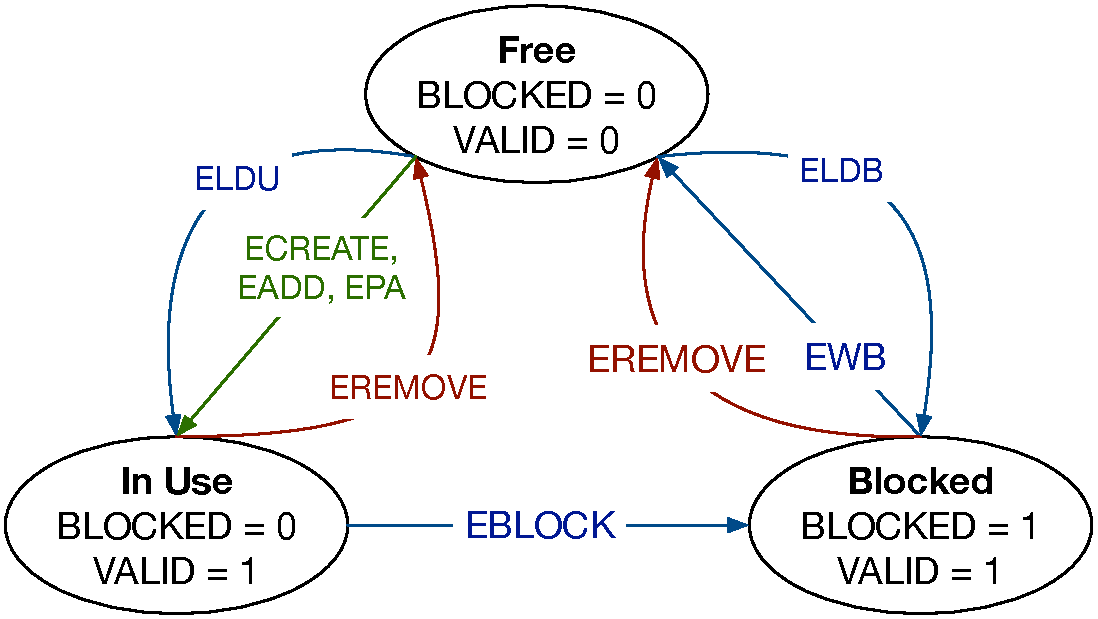
\includegraphics[width=80mm]{figures/sgx_page_states.pdf}
  \caption{
    The VALID and BLOCKED bits in an EPC page's EPCM entry can be in one of
    three states. \texttt{EADD} and its siblings allocate new EPC pages.
    \texttt{EREMOVE} permanently deallocates an EPC page. \texttt{EBLOCK}
    blocks an EPC page so it can be evicted using \texttt{EWB}. \texttt{ELDB}
    and \texttt{ELDU} load an evicted page back into the EPC.
  }
  \label{fig:sgx_page_states}
\end{figure}

Blocked pages are not considered accessible to enclaves. If an address
translation results in a blocked EPC page, the SGX implementation causes the
translation to result in a Page Fault~(\#PF,~\S~\ref{sec:faults}). This
guarantees that once a page is blocked, the CPU will not create any new TLB
entries pointing to it.

Furthermore, every SGX instruction makes sure that the EPC pages on which it
operates are not blocked. For example, \texttt{EENTER} ensures that the TCS
it is given is not blocked, that its enclave's SECS is not blocked, and that
every page in the current SSA is not blocked.

% Eviction of Enclave Pages: SDM S 39.5.3

In order to evict a batch of EPC pages, the OS kernel must first issue
\texttt{EBLOCK} instructions targeting them. The OS is also expected to remove
the EPC page's mapping from page tables, but is not trusted to do so.

After all the desired pages have been blocked, the OS kernel must execute an
\texttt{ETRACK} instruction, which directs the SGX implementation to keep track
of which logical processors have had their TLBs flushed. \texttt{ETRACK}
requires the virtual address of an enclave's SECS~(\S~\ref{sec:sgx_secs}). If
the OS wishes to evict a batch of EPC pages belonging to multiple enclaves, it
must issue an \texttt{ETRACK} for each enclave.

Following the \texttt{ETRACK} instructions, the OS kernel must induce enclave
exits on all the logical processors that are executing code inside the enclaves
that have been \texttt{ETRACK}ed. The SGX design expects that the OS will use
IPIs to cause AEXs in the logical processors whose TLBs must be flushed.

The EPC page eviction process is completed when the OS executes an \texttt{EWB}
instruction for each EPC page to be evicted. This instruction, which will be
fully described in \S~\ref{sec:sgx_ewb}, writes an encrypted version of the EPC
page to be evicted into DRAM, and then frees the page by clearing the VALID and
BLOCKED bits in its EPCM entry. Before carrying out its tasks, \texttt{EWB}
ensures that the EPC page that it targets has been blocked, and checks the
state set up by \texttt{ETRACK} to make sure that all the relevant TLBs have
been flushed.

An evicted page can be loaded back into the EPC via the \texttt{ELDU} and
\texttt{ELDB} instructions. Both instructions start up with a free EPC page and
a DRAM page that has the evicted contents of an EPC page, decrypt the DRAM
page's contents into the EPC page, and restore the corresponding EPCM entry.
The only difference between \texttt{ELDU} and \texttt{ELDB} is that the latter
sets the BLOCKED bit in the page's EPCM entry, whereas the former leaves it
cleared.

\texttt{ELDU} and \texttt{ELDB} resemble \texttt{ECREATE} and \texttt{EADD},
in the sense that they populate a free EPC page. Since the page that they
operate on was free, the SGX security model predicates that no TLB entries can
possibly target it. Therefore, these instructions do not require a mechanism
similar to \texttt{EBLOCK} or \texttt{ETRACK}.


\HeadingLevelC{The Version Array (VA)}
\label{sec:sgx_va}
\label{sec:sgx_epa}

% Version Array (VA): SDM S 38.18
% EPC and Management of EPC Pages: SDM S 39.5, 39.5.{2,3,4,5,6}

When \texttt{EWB} evicts the contents of an EPC, it creates an 8-byte
nonce~(\S~\ref{sec:freshness_crypto}) that Intel's documentation calls a
\textit{page version}. SGX's freshness guarantees are built on the assumption
that nonces are stored securely, so \texttt{EWB} stores the nonce that it
creates inside a \textit{Version Array}~(VA).

Version Arrays are EPC pages that are dedicated to storing nonces generated by
EWB. Each VA is divided into slots, and each slot is exactly large enough to
store one nonce. Given that the size of an EPC page is 4KB, and each nonce
occupies 8 bytes, it follows that each VA has 512 slots.

% EPA: SDM S 41.3

VA pages are allocated using the \texttt{EPA} instruction, which takes in the
virtual address of a free EPC page, and turns it into a Version Array with
empty slots. VA pages are identified by the PT\_VA type in their EPCM entries.
Like SECS pages, VA pages have the ENCLAVEADDRESS fields in their EPCM entries
set to zero, and cannot be accessed directly by any software, including
enclaves.

% EBLOCK, EREMOVE: SDM S 41.3

Unlike the other page types discussed so far, VA pages are not associated with
any enclave. This means they can be deallocated via \texttt{EREMOVE} without
any restriction. However, freeing up a VA page whose slots are in use
effectively discards the nonces in those slots, which results in losing the
ability to load the corresponding evicted pages back into the EPC. Therefore,
it is unlikely that a correct OS implementation will ever call \texttt{EREMOVE}
on a VA with non-free slots.

% EPA, EWB: SDM S 41.3

According to the pseudo-code for \texttt{EPA} and \texttt{EWB} in the SDM, SGX
uses the zero value to represent the free slots in a VA, implying that all the
generated nonces have to be non-zero. This also means that \texttt{EPA}
initializes a VA simply by zeroing the underlying EPC page. However, since
software cannot access a VA's contents, neither the use of a special value, nor
the value itself is architectural.


\HeadingLevelC{Enclave IDs}
\label{sec:sgx_eid}

The \texttt{EWB} and \texttt{ELDU} / \texttt{ELDB} instructions use an
\textit{enclave ID}~(EID) to identify the enclave that owns an evicted page.
The EID has the same purpose as the ENCLAVESECS~(\S~\ref{sec:sgx_epcm}) field
in an EPCM entry, which is also used to identify the enclave that owns an EPC
page. This section explains the need for having two values represent the same
concept by comparing the two values and their uses.

% Enclave Page Cache Map (EPCM): SDM S 37.5.1, SDM S 38.19

The SDM states that ENCLAVESECS field in an EPCM entry is used to identify the
SECS of the enclave owning the associated EPC page, but stops short of
describing its format. In theory, the ENCLAVESECS field can change its
representation between SGX implementations since SGX instructions never expose
its value to software.

% ENCLAVESECS compared with CR_ACTIVE_SECS
% EENTER: TMP_SECS <- address of SECS for TCS; CR_ACTIVE_SECS <- TMP_SECS

However, we will later argue that the most plausible representation of the
ENCLAVESECS field is the physical address of the enclave's SECS. Therefore, the
ENCLAVESECS value associated with a given enclave will change if the enclave's
SECS is evicted from the EPC and loaded back at a different location. It
follows that the ENCLAVESECS value is only suitable for identifying an enclave
while its SECS remains in the EPC.

% Internal CREGs: SDM S 41.1.4
% ECREATE: SDM S 41.3

According to the SDM, the EID field is a 64-bit field stored in an enclave's
SECS. \texttt{ECREATE}'s pseudocode in the SDM reveals that an enclave's ID is
generated when the SECS is allocated, by atomically incrementing a global
counter. Assuming that the counter does not roll over\footnote{A 64-bit counter
incremented at 4Ghz would roll over in slightly more than 136 years}, this
process guarantees that every enclave created during a power cycle has a unique
EID.

Although the SDM does not specifically guarantee this, the EID field in an
enclave's SECS does not appear to be modified by any instruction. This makes
the EID's value suitable for identifying an enclave throughout its lifetime,
even across evictions of its SECS page from the EPC.


\HeadingLevelC{Evicting an EPC Page}
\label{sec:sgx_ewb}

The system software evicts an EPC page using the \texttt{EWB} instruction,
which produces all the data needed to restore the evicted page at a later time
via the \texttt{ELDU} instruction, as shown in Figure~\ref{fig:sgx_eviction}.

\begin{figure}[hbt]
  \centering
  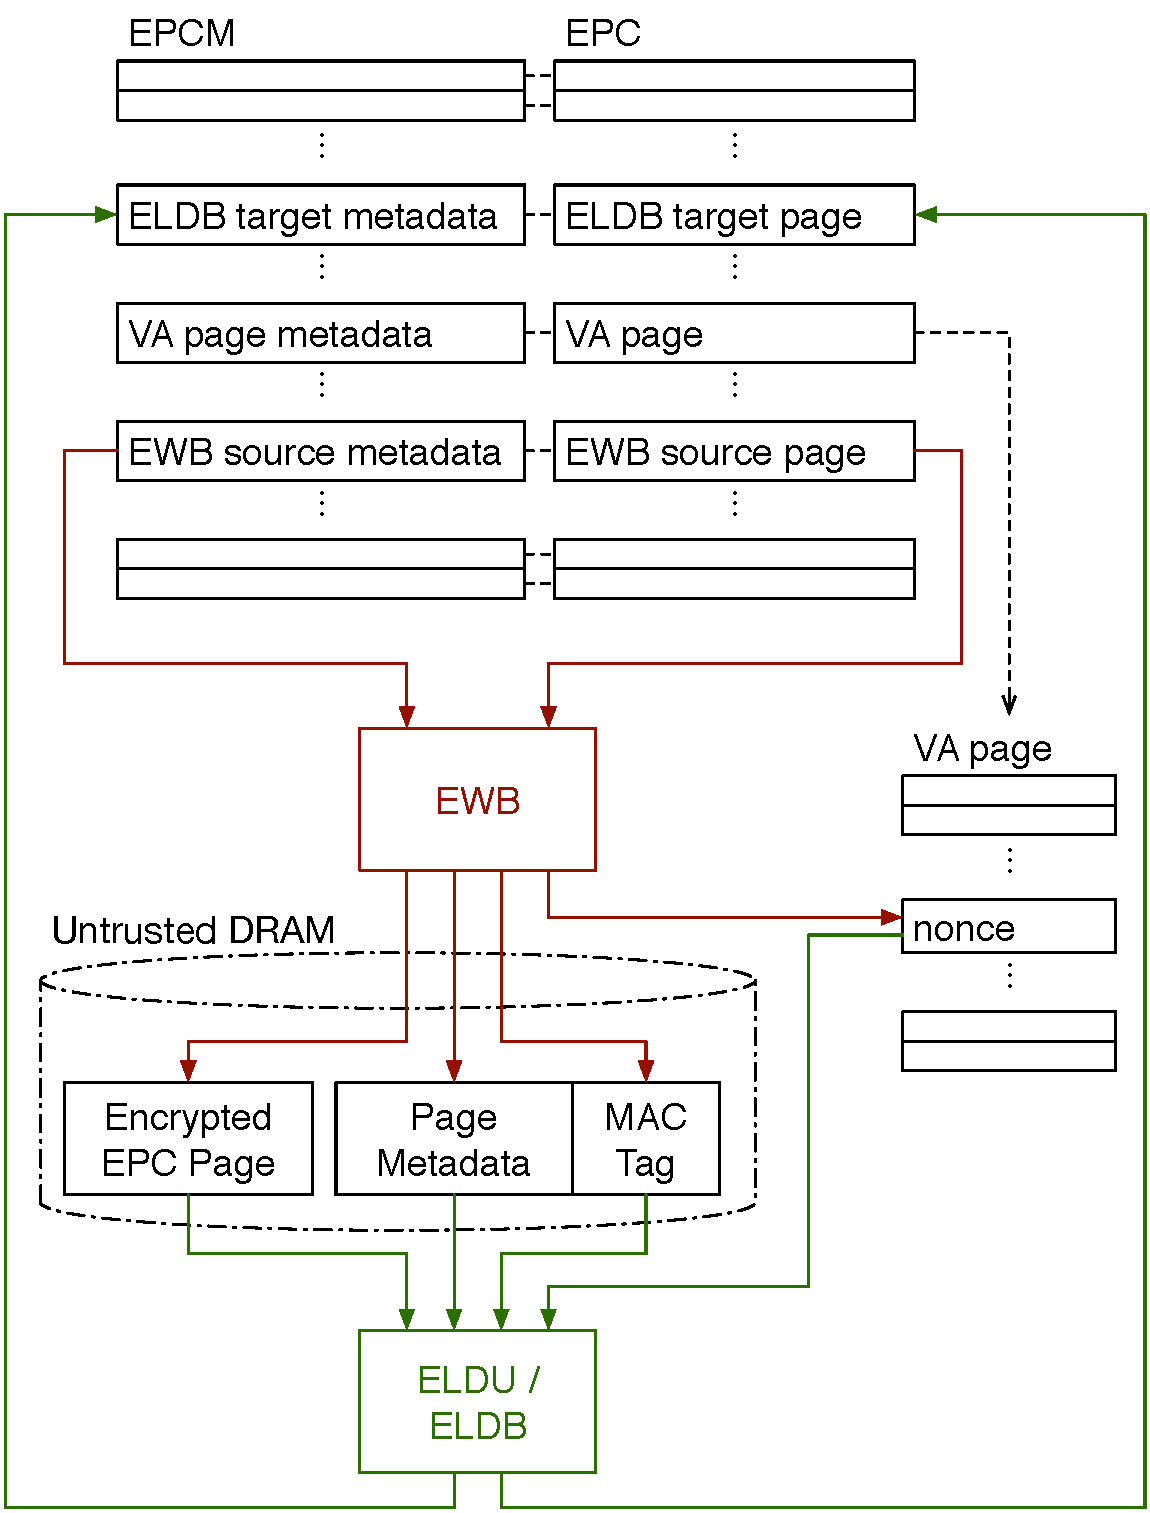
\includegraphics[width=85mm]{figures/sgx_eviction.pdf}
  \caption{
    The \texttt{EWB} instruction outputs the encrypted contents of the
    evicted EPC page, a subset of the fields in the page's EPCM entry, a
    MAC tag, and a nonce. All this information is used by the \texttt{ELDB} or
    \texttt{ELDU} instruction to load the evicted page back into the EPC, with
    privacy, integrity and freshness guarantees.
  }
  \label{fig:sgx_eviction}
\end{figure}

% EWB: SDM S 41.3

\texttt{EWB}'s output consists of an encrypted version of the evicted EPC
page's contents, a subset of the fields in the EPCM entry corresponding to the
page, the nonce discussed in \S~\ref{sec:sgx_va}, and a message authentication
code~(MAC,~\S~\ref{sec:integrity_crypto}) tag. With the exception of the nonce,
\texttt{EWB} writes its output in DRAM outside the PRM area, so the system
software can choose to further evict it to disk.

The EPC page contents is encrypted, to protect the privacy of the enclave's
data while the page is stored in the untrusted DRAM outside the PRM range.
Without the use of encryption, the system software could learn the contents of
an EPC page by evicting it from the EPC.

% Security Information (SECINFO): SDM S 38.11, S 38.11.{1,2}

The page metadata is stored in a \textit{Page Information}~(PAGEINFO)
structure, illustrated in Figure~\ref{fig:sgx_ewb_pageinfo}. This structure is
similar to the PAGEINFO structure described in \S~\ref{sec:sgx_eadd} and
depicted in Figure~\ref{fig:sgx_pageinfo}, except that the SECINFO field has
been replaced by a PCMD field, which contains the virtual address of a
\textit{Page Crypto Metadata}~(PCMD) structure.

\begin{figure}[hbt]
  \centering
  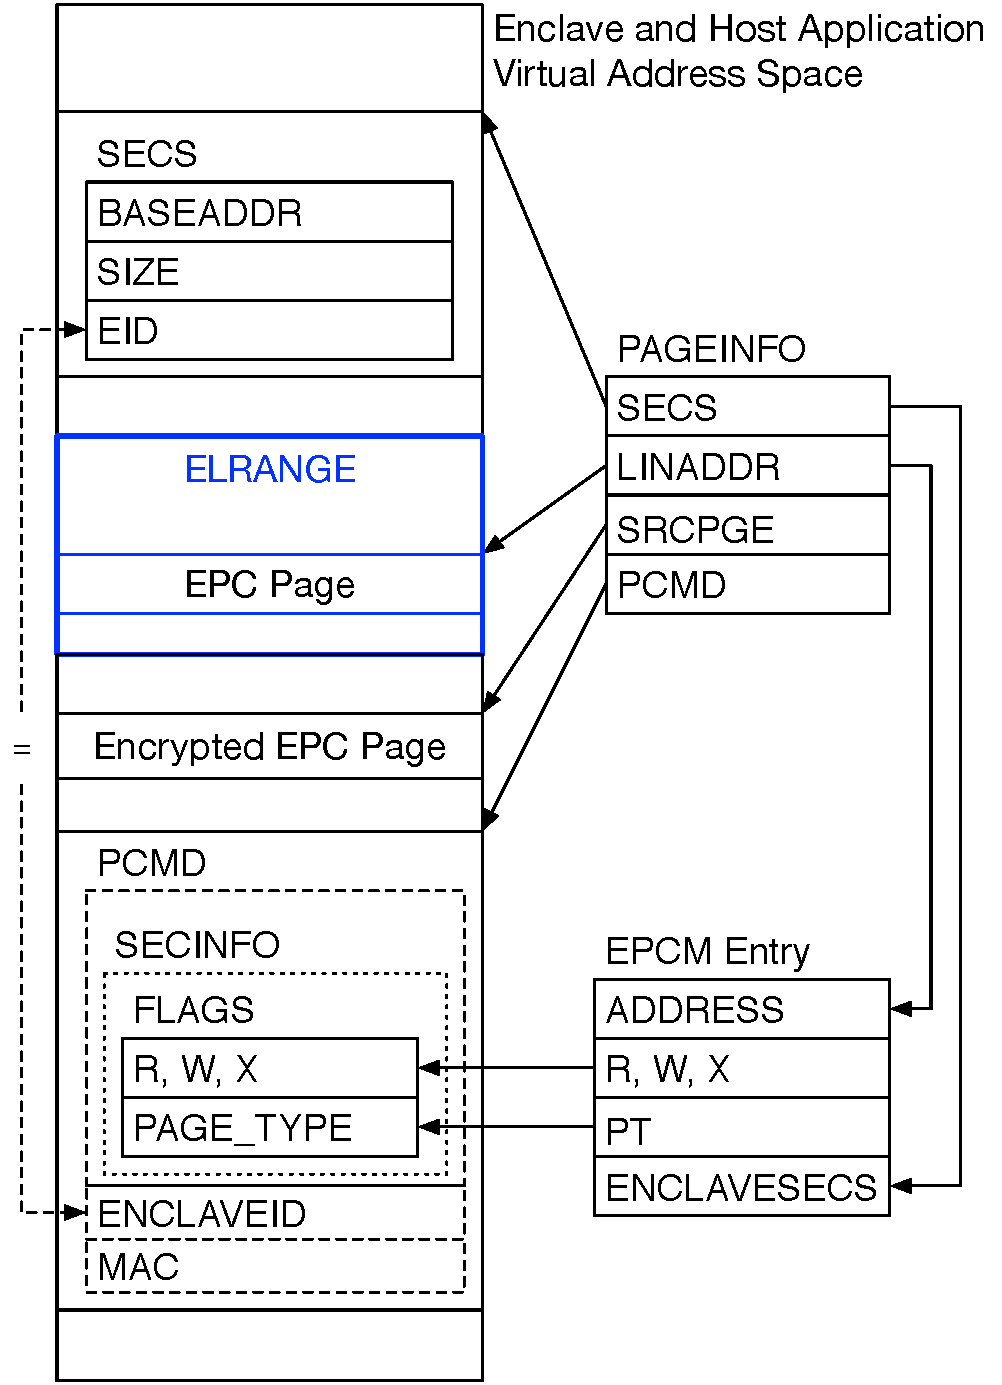
\includegraphics[width=75mm]{figures/sgx_ewb_pageinfo.pdf}
  \caption{
    The PAGEINFO structure used by the \texttt{EWB} and \texttt{ELDU} /
    \texttt{ELDB} instructions
  }
  \label{fig:sgx_ewb_pageinfo}
\end{figure}

The LINADDR field in the PAGEINFO structure is used to store the ADDRESS field
in the EPCM entry, which indicates the virtual address intended for accessing
the page. The PCMD structure embeds the \textit{Security Information}~(SECINFO)
described in \S~\ref{sec:sgx_eadd}, which is used to store the page type~(PT)
and the access permission flags~(R, W, X) in the EPCM entry. The PCMD structure
also stores the enclave's ID~(EID,~\S~\ref{sec:sgx_eid}). These fields are
later used by \texttt{ELDU} or \texttt{ELDB} to populate the EPCM entry for the
EPC page that is reloaded.

The metadata described above is stored unencrypted, so the OS has the option of
using the information inside as-is for its own bookkeeping. This has no
negative impact on security, because the metadata is not confidential. In fact,
with the exception of the enclave ID, all the metadata fields are specified by
the system software when \texttt{ECREATE} is called. The enclave ID is only
useful for identifying the enclave that the EPC page belongs to, and the system
software already has this information as well.

Asides from the metadata described above, the PCMD structure also stores the
MAC tag generated by \texttt{EWB}. The MAC tag covers the authenticity of the
EPC page contents, the metadata, and the nonce. The MAC tag is checked by
\texttt{ELDU} and \texttt{ELDB}, which will only load an evicted page back into
the EPC if the MAC verification confirms the authenticity of the page data,
metadata, and nonce. This security check protects against the page swapping
attacks described in \S~\ref{sec:page_swapping_attacks}.

% Eviction of an SECS Page: SDM S 39.5.5

Similarly to \texttt{EREMOVE}, \texttt{EWB} will only evict the EPC page
holding an enclave's SECS if there is no other EPCM entry whose ENCLAVESECS
field references the SECS. At the same time, as an optimization, the SGX
implementation does not perform \texttt{ETRACK}-related checks when evicting a
SECS. This is safe because a SECS is only evicted if the EPC has no pages
belonging to the SECS' enclave, which implies that there isn't any TCS
belonging to the enclave in the EPC, so no processor can be executing enclave
code.

% Eviction of a Version Array Page: SDM S 39.5.6

The pages holding Version Arrays can be evicted, just like any other EPC page.
VA pages are never accessible by software, so they can't have any TLB entries
pointing to them. Therefore, \texttt{EWB} evicts VA pages without performing
any \texttt{ETRACK}-related checks. The ability to evict VA pages has profound
implications that will be discussed in \S~\ref{sec:sgx_eviction_trees}.

\texttt{EWB}'s data flow, shown in detail in Figure~\ref{fig:sgx_ewb}, has an
aspect that can be confusing to OS developers. The instruction reads the
virtual address of the EPC page to be evicted from a register (RBX) and writes
it to the LINADDR field of the PAGEINFO structure that it is provided. The
separate input (RBX) could have been removed by providing the EPC page's address
in the LINADDR field.

\begin{figure}[hbt]
  \centering
  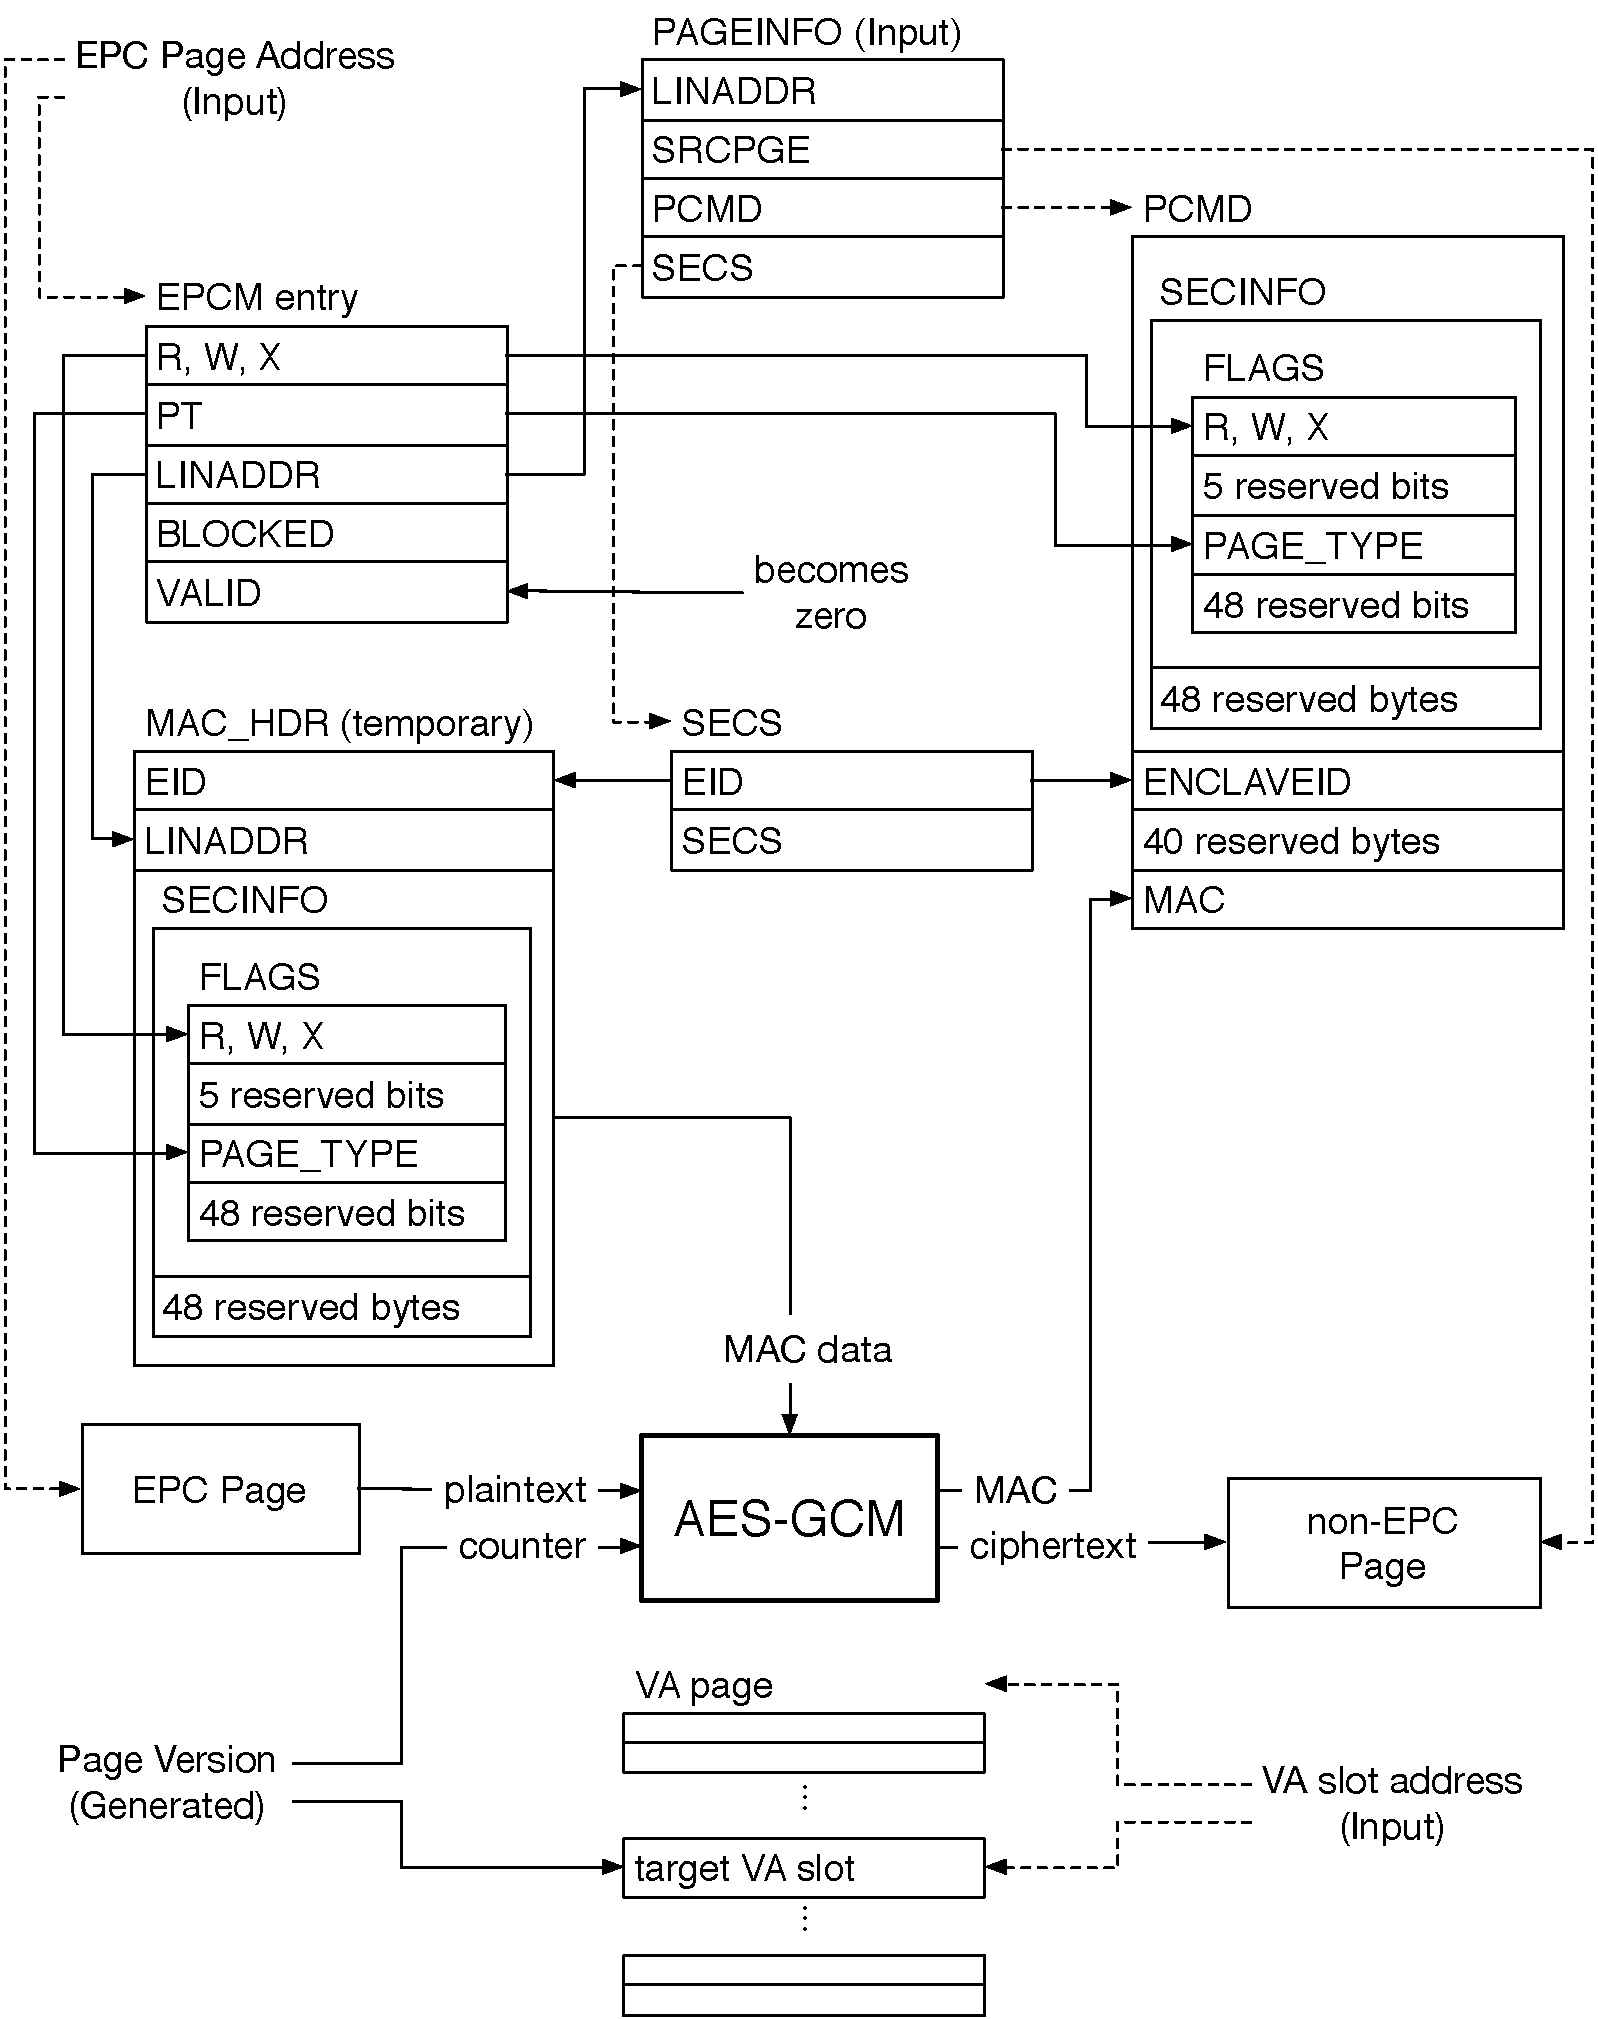
\includegraphics[width=85mm]{figures/sgx_ewb.pdf}
  \caption{
    The data flow of the EWB instruction that evicts an EPC page. The page's
    content is encrypted in a non-EPC RAM page. A nonce is created and saved
    in an empty slot inside a VA page. The page's EPCM metadata and a MAC
    are saved in a separate area in non-EPC memory.
  }
  \label{fig:sgx_ewb}
\end{figure}

% Enclave page protection while not in EPC uses a version tree, GMAC etc.
%   US 8,972,746 B2 - 23:13-67, 24:1-19, 24:31-46, 24:65-67,


\HeadingLevelC{Loading an Evicted Page Back into EPC}

% AEX Operational Detail: SDM S 40.4.1

After an EPC page belonging to an enclave is evicted, any attempt to access the
page from enclave code will result in a Page Fault~(\#PF,~\S~\ref{sec:faults}).
The \#PF will cause the logical processor to exit enclave mode via
AEX~(\S~\ref{sec:sgx_aex}), and then invoke the OS kernel's page fault handler.

Page faults receive special handling from the AEX process. While leaving the
enclave, the AEX logic specifically checks if the hardware exception that
triggered the AEX was \#PF. If that is the case, the AEX implementation clears
the least significant 12 bits of the CR2 register, which stores the virtual
address whose translation caused a page fault.

In general, the OS kernel's page handler needs to be able to extract the
virtual page number~(VPN,~\S~\ref{sec:paging_vpn}) from CR2, so that it knows
which memory page needs to be loaded back into DRAM. The OS kernel may also be
able to use the 12 least significant address bits, which are not part of the
VPN, to better predict the application software's memory access patterns.
However, unlike the bits that make up the VPN, the bottom 12 bits are not
absolutely necessary for the fault handler to carry out its job. Therefore,
SGX's AEX implementation clears these 12 bits, in order to limit the amount of
information that is learned by the page fault handler.

% Loading an Enclave Page: SDM S 39.5.4
% TODO: page fault -> AEX -> ELDB / ELDU

When the OS page fault handler examines the address in the CR2 register and
determines that the faulting address is inside the EPC, it is generally
expected to use the \texttt{ELDU} or \texttt{ELDB} instruction to load the
evicted page back into the EPC. If the outputs of \texttt{EWB} have been
evicted from DRAM to a slower storage medium, the OS kernel will have to read
the outputs back into DRAM before invoking \texttt{ELDU} / \texttt{ELDB}.

\texttt{ELDU} and \texttt{ELDB} verify the MAC tag produced by \texttt{EWB},
described in \S~\ref{sec:sgx_ewb}. This prevents the OS kernel from performing
the page swapping-based active address translation attack described in
\S~\ref{sec:page_swapping_attacks}.


\HeadingLevelC{Eviction Trees}
\label{sec:sgx_eviction_trees}

The SGX design allows VA pages to be evicted from the EPC, just like enclave
pages. When a VA page is evicted from EPC, all the nonces stored by the VA
slots become inaccessible to the processor. Therefore, the evicted pages
associated with these nonces cannot be restored by \texttt{ELDB} until the
OS loads the VA page back into the EPC.

In other words, an evicted page depends on the VA page storing its nonce, and
cannot be loaded back into the EPC until the VA page is reloaded as well.
The dependency graph created by this relationship is a forest of
\texttt{eviction trees}. An eviction tree, shown in
Figure~\ref{fig:sgx_eviction_tree}, has enclave EPC pages as leaves, and VA
pages as inner nodes. A page's parent is the VA page that holds its nonce.
Since \texttt{EWB} always outputs a nonce in a VA page, the root node of each
eviction tree is always a VA page in the EPC.

\begin{figure}[hbt]
  \centering
  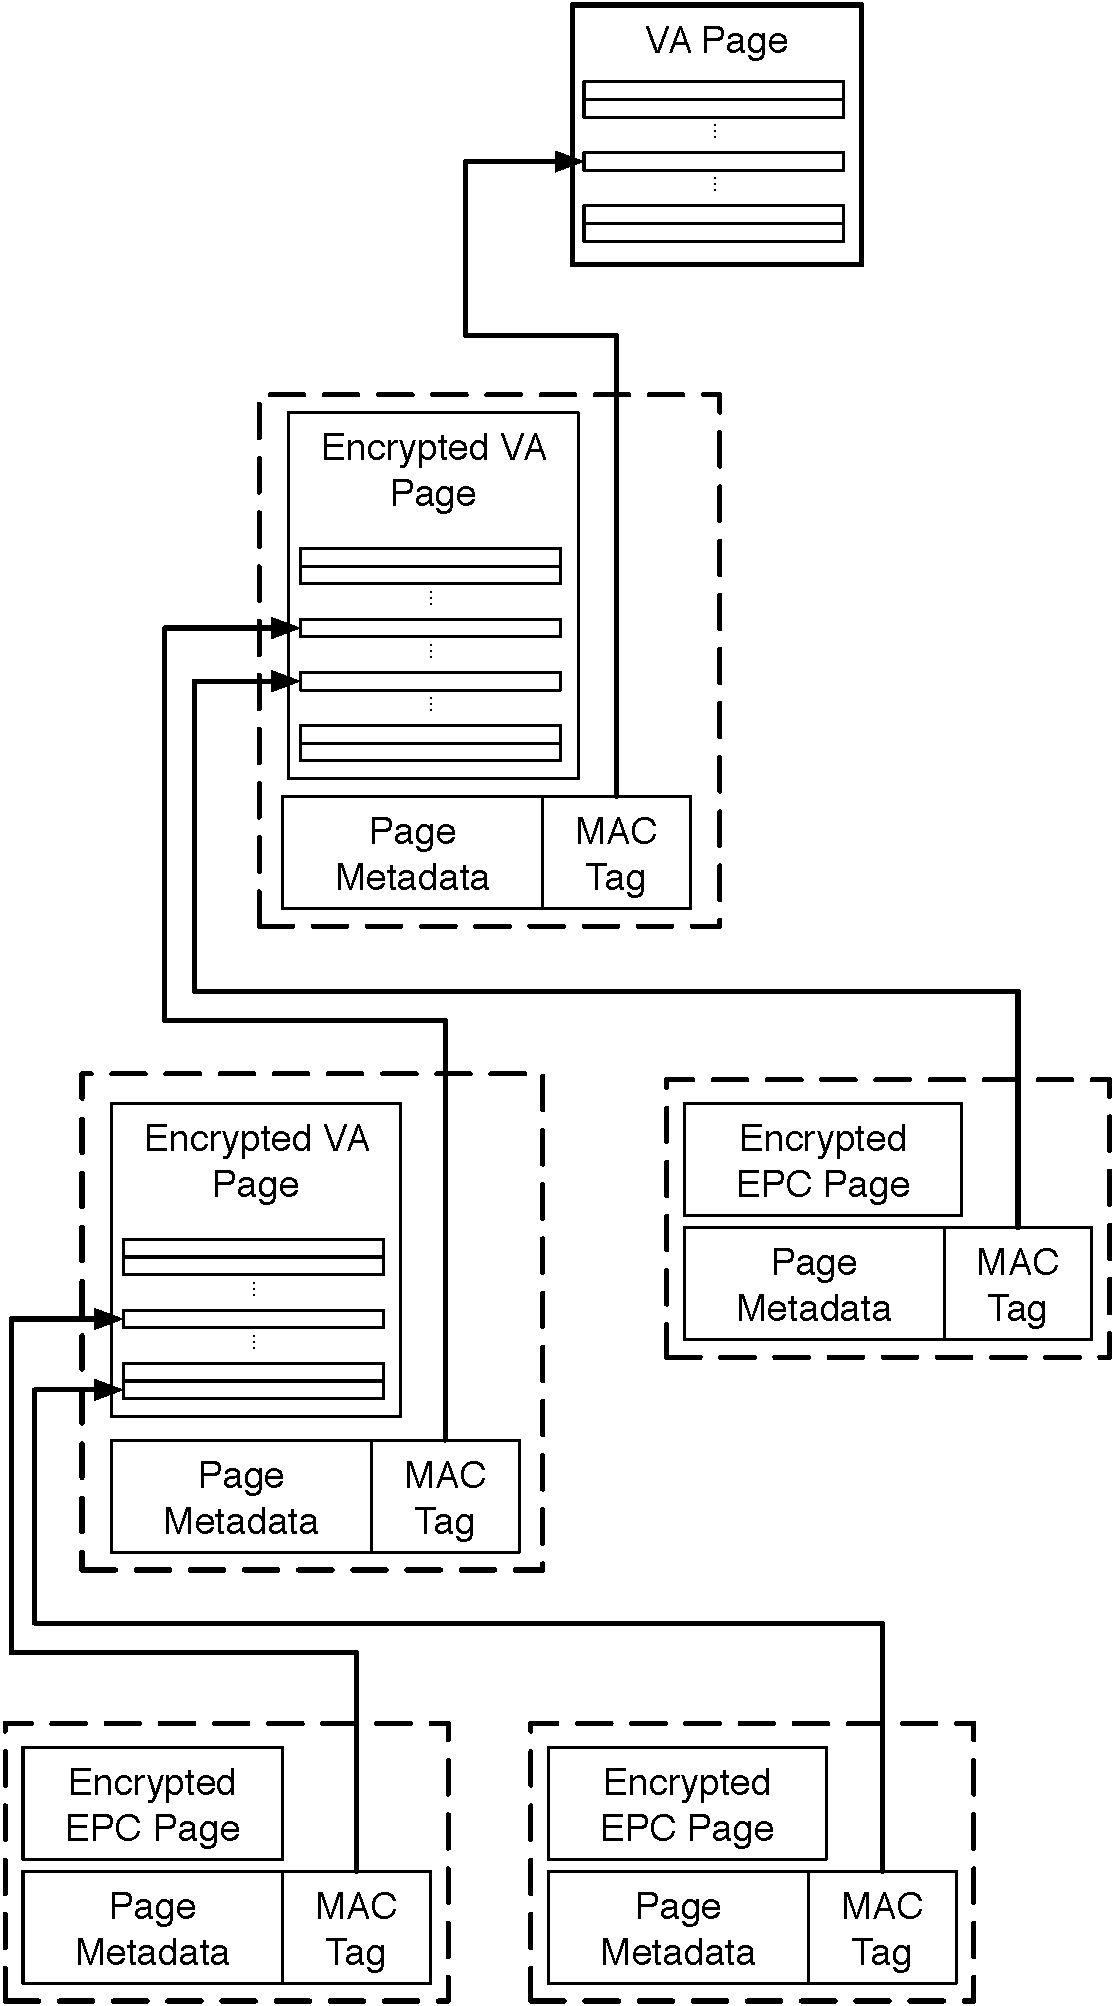
\includegraphics[width=80mm]{figures/sgx_eviction_tree.pdf}
  \caption{
    A version tree formed by evicted VA pages and enclave EPC pages. The
    enclave pages are leaves, and the VA pages are inner nodes. The OS controls
    the tree's shape, which impacts the performance of evictions, but not their
    correctness.
  }
  \label{fig:sgx_eviction_tree}
\end{figure}

A straightforward inductive argument shows that when an OS wishes to load an
evicted enclave page back into the EPC, it needs to load all the VA pages on
the path from the eviction tree's root to the leaf corresponding to the enclave
page. Therefore, the number of page loads required to satisfy a page fault
inside the EPC depends on the shape of the eviction tree that contains the
page.

The SGX design leaves the OS in complete control of the shape of the eviction
trees. This has no negative impact on security, as the tree shape only impacts
the performance of the eviction scheme, and not its correctness.

\subsection{SGX Enclave Measurement}
\label{sec:sgx_measurement}
\label{sec:sgx_mrenclave}

SGX implements a software attestation scheme that follows the general
principles outlined in \S~\ref{sec:generic_software_attestation}. For the
purposes of this section, the most relevant principle is that a remote party
authenticates an enclave based on its measurement, which is intended to
identify the software that is executing inside the enclave. The remote party
compares the enclave measurement reported by the trusted hardware with an
expected measurement, and only proceeds if the two values match.

% Enclave Measurement: SDM S 39.4.1

\S~\ref{sec:sgx_enclave_lifecycle} explains that an SGX enclave is built using
the \texttt{ECREATE}~(\S~\ref{sec:sgx_ecreate}),
\texttt{EADD}~(\S~\ref{sec:sgx_eadd}) and \texttt{EEXTEND} instructions.
After the enclave is initialized via
\texttt{EINIT}~(\S~\ref{sec:sgx_einit_overview}) the instructions mentioned
above cannot be used anymore. As the SGX measurement scheme follows the
principles outlined in \S~\ref{sec:generic_measurement}, the measurement of an
SGX enclave is obtained by computing a secure
hash~(\S~\ref{sec:integrity_crypto}) over the inputs to the \texttt{ECREATE},
\texttt{EADD} and \texttt{EEXTEND} instructions used to create the enclave and
load the initial code and data into its memory. \texttt{EINIT} finalizes the
hash that represents the enclave's measurement.

Along with the enclave's contents, the enclave author is expected to specify
the sequence of instructions that should be used in order to create an enclave
whose measurement will match the expected value used by the remote party in the
software attestation process. The \texttt{.so} and \texttt{.dll} dynamically
loaded library file formats, which are SGX's intended enclave delivery methods,
already include informal specifications for loading algorithms. We expect the
informal loading specifications to serve as the starting points for
specifications that prescribe the exact sequences of SGX instructions that
should be used to create enclaves from \texttt{.so} and \texttt{.dll} files.

As argued in \S~\ref{sec:generic_measurement}, an enclave's measurement is
computed using a secure hashing algorithm, so the system software can only
build an enclave that matches an expected measurement by following the exact
sequence of instructions specified by the enclave's author.

% SGX Enclave Control Structure (SECS): SDM S 38.7, S 38.7.1
% MRENCLAVE: SDM S 39.4.1.1

The SGX design uses the 256-bit SHA-2~\cite{fips2015shs} secure hash function
to compute its measurements. SHA-2 is a block hash
function~(\S~\ref{sec:integrity_crypto}) that operates on 64-byte blocks, uses
a 32-byte internal state, and produces a 32-byte output. Each enclave's
measurement is stored in the MRENCLAVE field of the enclave's SECS. The 32-byte
field stores the internal state and final output of the 256-bit SHA-2 secure
hash function.


\subsubsection{Measuring \texttt{ECREATE}}
\label{sec:sgx_ecreate_mrenclave}

% ECREATE: SDM S 41.3

The \texttt{ECREATE} instruction, overviewed in \S~\ref{sec:sgx_ecreate},
first initializes the MRENCLAVE field in the newly created SECS using the
256-bit SHA-2 initialization algorithm, and then extends the hash with
the 64-byte block depicted in Table~\ref{fig:ecreate_mrenclave}.

\begin{table}[hbt]
  \centering
  \begin{tabularx}{\columnwidth}{| r | r | X |}
  \hline
  \textbf{Offset} & \textbf{Size} & \textbf{Description}\\
  \hline
  0 & 8 & "ECREATE\textbackslash{}0" \\
  \hline
  8 & 8 & SECS.SSAFRAMESIZE (\S~\ref{sec:sgx_ssa}) \\
  \hline
  16 & 8 & SECS.SIZE (\S~\ref{sec:sgx_elrange}) \\
  \hline
  32 & 8 & 32 zero (0) bytes \\
  \hline
  \end{tabularx}
  \caption{
    64-byte block extended into MRENCLAVE by \texttt{ECREATE}
  }
  \label{fig:ecreate_mrenclave}
\end{table}

The enclave's measurement does not include the BASEADDR field. The omission is
intentional, as it allows the system software to load an enclave at any virtual
address inside a host process that satisfies the ELRANGE
restrictions~(\S~\ref{sec:sgx_elrange}), without changing the enclave's
measurement. This feature can be combined with a compiler that generates
position-independent enclave code to obtain relocatable enclaves.

The enclave's measurement includes the \texttt{SSAFRAMESIZE} field, which
guarantees that the SSAs~\ref{sec:sgx_ssa} created by AEX and used by
\texttt{EENTER}~(\S~\ref{sec:sgx_eenter}) and
\texttt{ERESUME}~(\S~\ref{sec:sgx_eresume}) have the size that is expected by
the enclave's author. Leaving this field out of an enclave's measurement would
allow a malicious enclave loader to attempt to attack the enclave's security
checks by specifying a bigger SSAFRAMESIZE than the enclave's author intended,
which could cause the SSA contents written by an AEX to overwrite the enclave's
code or data.

\subsubsection{Measuring Enclave Attributes}
\label{sec:sgx_ecreate_mrenclave_no_attributes}

The enclave's measurement does not include the enclave
attributes~(\S~\ref{sec:sgx_secs_attributes}), which are specified in the
ATTRIBUTES field in the SECS. Instead, it is included directly in the
information that is covered by the attestation signature, which will be
discussed in \S~\ref{sec:sgx_ereport}.

The SGX software attestation definitely needs to cover the enclave attributes.
For example, if XFRM~(\S~\ref{sec:sgx_secs_attributes}, \S~\ref{sec:sgx_ssa})
would not be covered, a malicious enclave loader could attempt to subvert an
enclave's security checks by setting XFRM to a value that enables architectural
extensions which change the semantics of instructions used by the enclave, but
still produces an \texttt{XSAVE} output that fits in SSAFRAMESIZE.

The special treatment applied to the ATTRIBUTES SECS field seems questionable
from a security standpoint, as it adds extra complexity to the software
attestation verifier, which translates into more opportunities for exploitable
bugs. This decision also adds complexity to the SGX software attestation
design, which is described in \S~\ref{sec:sgx_attestation}.

The most likely reason why the SGX design decided to go this route, despite the
concerns described above, is the wish to be able to use a single measurement to
represent an enclave that can take advantage of some architectural extensions,
but can also perform its task without them.

Consider, for example, an enclave that performs image processing using a
library such as OpenCV, which has routines optimized for SSE and AVX, but also
includes generic fallbacks for processors that do not have these features. The
enclave's author will likely wish to allow an enclave loader to set bits 1
(SSE) and 2 (AVX) to either true or false. If ATTRIBUTES (and, by extension,
XFRM) was a part of the enclave's measurement, the enclave author would have to
specify that the enclave has 4 valid measurements. In general, allowing $n$
architectural extensions to be used independently will result in $2^n$ valid
measurements.


\subsubsection{Measuring \texttt{EADD}}
\label{sec:sgx_eadd_mrenclave}

% EADD and EEXTEND Interaction: SDM S 39.1.1
% EADD: SDM S 41.3

The \textit{EADD} instruction, described in \S~\ref{sec:sgx_eadd}, extends the
SHA-2 hash in MRENCLAVE with the 64-byte block shown in
Table~\ref{fig:eadd_mrenclave}.

\begin{table}[hbt]
  \centering
  \begin{tabularx}{\columnwidth}{| r | r | X |}
  \hline
  \textbf{Offset} & \textbf{Size} & \textbf{Description}\\
  \hline
  0 & 8 &
  "EADD\textbackslash{}0\textbackslash{}0\textbackslash{}0\textbackslash{}0" \\
  \hline
  8 & 8 & ENCLAVEOFFSET \\
  \hline
  16 & 48 & SECINFO (first 48 bytes) \\
  \hline
  \end{tabularx}
  \caption{
    64-byte block extended into MRENCLAVE by \texttt{EADD}. The ENCLAVEOFFSET
    is computed by subtracting the BASEADDR in the enclave's SECS from the
    LINADDR field in the PAGEINFO structure.
  }
  \label{fig:eadd_mrenclave}
\end{table}

The address included in the measurement is the address where the
\texttt{EADD}ed page is expected to be mapped in the enclave's virtual address
space. This ensures that the system software sets up the enclave's virtual
memory layout according to the enclave author's specifications. If a malicious
enclave loader attempts to set up the enclave's layout incorrectly, perhaps in
order to mount an active address translation
attack~(\S~\ref{sec:memory_mapping_attacks}), the loaded enclave's measurement
will differ from the measurement expected by the enclave's author.

The virtual address of the newly created page is measured relatively to the
start of the enclave's ELRANGE. In other words, the value included in the
measurement is LINADDR - BASEADDR. This makes the enclave's measurement
invariant to BASEADDR changes, which is desirable for relocatable enclaves.
Measuring the relative addresses still preserves all the information about the
memory layout inside ELRANGE, and therefore has no negative security impact.

\texttt{EADD} also measures the first 48 bytes of the SECINFO
structure~(\S~\ref{sec:sgx_eadd}) provided to \texttt{EADD}, which contains the
page type (PT) and access permissions (R, W, X) field values used to initialize
the page's EPCM entry. By the same argument as above, including these values in
the measurement guarantees that the memory layout built by the system software
loading the enclave matches the specifications of the enclave author.

The EPCM field values mentioned above take up less than one byte in the SECINFO
structure, and the rest of the bytes are reserved and expected to be
initialized to zero. This leaves plenty of expansion room for future SGX
features.

The most notable omission from Table~\ref{fig:eadd_mrenclave} is the data used
to initialize the newly created EPC page. Therefore, the measurement data
contributed by \texttt{EADD} guarantees that the enclave's memory layout
will have pages allocated with prescribed access permissions at the desired
virtual addresses. However, the measurements don't cover the code or data
loaded in these pages.

For example, \texttt{EADD}'s measurement data guarantees that an enclave's
memory layout consists of three executable pages followed by five writable data
pages, but it does not guarantee that any of the code pages contains the
code supplied by the enclave's author.


\subsubsection{Measuring \texttt{EEXTEND}}
\label{sec:sgx_eextend}

% EEXTEND: SDM S 41.3

The \texttt{EEXTEND} instruction exists solely for the reason of measuring data
loaded inside the enclave's EPC pages. The instruction reads in a virtual
address, and extends the enclave's measurement hash with the five 64-byte
blocks in Table~\ref{fig:eextend_mrenclave}, which have the effect of
guaranteeing the contents of a 256-byte chunk of data in the enclave's memory.

\begin{table}[hbt]
  \centering
  \begin{tabularx}{\columnwidth}{| r | r | X |}
  \hline
  \textbf{Offset} & \textbf{Size} & \textbf{Description}\\
  \hline
  0 & 8 & "EEXTEND\textbackslash{}0" \\
  \hline
  8 & 8 & ENCLAVEOFFSET \\
  \hline
  16 & 48 & 48 zero (0) bytes \\
  \hline
  \hline
  64 & 64 & bytes 0 - 64 in the chunk \\
  \hline
  \hline
  128 & 64 & bytes 64 - 128 in the chunk \\
  \hline
  \hline
  192 & 64 & bytes 128 - 192 in the chunk \\
  \hline
  \hline
  256 & 64 & bytes 192 - 256 in the chunk \\
  \hline
  \end{tabularx}
  \caption{
    64-byte blocks extended into MRENCLAVE by \texttt{EEXTEND}. The
    ENCLAVEOFFSET is computed by subtracting the BASEADDR in the enclave's SECS
    from the LINADDR field in the PAGEINFO structure.
  }
  \label{fig:eextend_mrenclave}
\end{table}

Before examining the details of \texttt{EEXTEND}, we note that SGX's security
guarantees only hold when the contents of the enclave's key pages is measured.
For example, \texttt{EENTER}~(\S~\ref{sec:sgx_eenter}) is only guaranteed to
perform controlled jumps inside an enclave's code if the contents of all the
Thread Control Structure~(TCS,~\S~\ref{sec:sgx_tcs}) pages is measured.
Otherwise, a malicious enclave loader can change the OENTRY
field~(\S~\ref{sec:sgx_tcs}, \S~\ref{sec:sgx_eenter}) in a TCS while building
the enclave, and then a malicious OS can use the TCS to perform an arbitrary
jump inside enclave code.

By the same argument, all the enclave's code should be measured by
\texttt{EEXTEND}. Any code fragment that is not measured can be replaced by a
malicious enclave loader.

Given these pitfalls, it is surprising that the SGX design opted to decouple
the virtual address space layout measurements done by \texttt{EADD} from the
memory content measurements done by \texttt{EEXTEND}. The decoupling does
provide a benefit, namely the ability to load un-measured user input into an
enclave while it is being built. However, this benefit only translates into a
small performance improvement, because enclaves can alternatively be designed
to copy the user input from untrusted DRAM after being initialized. At the same
time, the decoupling opens up the possibility of relying on an enclave that
provides no meaningful security guarantees, due to not measuring all the
important data via \texttt{EEXTEND} calls.

A mitigating circumstance for the \texttt{EADD} / \texttt{EEXTEND} separation
is that the SGX design seems to expect enclaves to be authored using the same
tools that build today's dynamically loaded modules. Such tools would easily be
able to identify the enclave data that needs to be measured.

It is correct and meaningful, from a security perspective, to have the message
blocks provided by \texttt{EEXTEND} to the hash function include the address of
the 256-byte chunk, in addition to the contents of the data. If the address
were not included, a malicious enclave loader could mount the memory mapping
attack described in \S~\ref{sec:memory_mapping_attacks} and illustrated in
Figure~\ref{fig:active_mapping_attack}.

More specifically, the malicious loader would \texttt{EADD} the
\texttt{errorOut} page contents at the virtual address intended for
\texttt{disclose}, \texttt{EADD} the \texttt{disclose} page contents at the
virtual address intended for \texttt{errorOut}, and then \texttt{EEXTEND} the
pages in the wrong order. If \texttt{EEXTEND} would not include the address of
the data chunk that is measured, the steps above would yield the same
measurement as the correctly constructed enclave.

% SGX Enclave Control Structure (SECS): SDM S 38.7, S 38.7.1

The last aspect of \texttt{EEXTEND} worth analyzing is its support for
relocating enclaves. Similarly to \texttt{EADD}, the virtual address measured
by \texttt{EEXTEND} is relative to the enclave's BASEADDR. Furthermore, the
only SGX structure whose content is expected to be measured by \texttt{EEXTEND}
is the TCS. The SGX design has carefully used relative addresses for all the
TCS fields that represent enclave addresses, which are OENTRY, OFSBASGX and
OGSBASGX.


\subsubsection{Measuring \texttt{EINIT}}

% EINIT: SDM S 41.3

The \texttt{EINIT} instruction~(\S~\ref{sec:sgx_einit_overview}) concludes the
enclave building process. After \texttt{EINIT} is successfully invoked on an
enclave, the enclave's contents is ``sealed'', meaning that the system software
cannot use the \texttt{EADD} instruction to load code and data into the
enclave, and cannot use the \texttt{EEXTEND} instruction to update the
enclave's measurement.

\texttt{EINIT} uses the SHA-2 finalization
algorithm~(\S~\ref{sec:integrity_crypto}) on the MRENCLAVE field of the
enclave's SECS. After \texttt{EINIT}, the field no longer stores the
intermediate state of the SHA-2 algorithm, and instead stores the final output
of the secure hash function. This value remains constant after \texttt{EINIT}
completes, and is included in the attestation signature produced by the
SGX software attestation process.

\section{Security Model}
\label{sec:attestation}

THe central context of SGX is the \textit{enclave}, a protected environment
that contains the code and data pertaining to a security-sensitive computation.
An SGX-enabled processor protects the integrity and privacy of the computation
inside an enclave by isolating the enclave's code and data from the outside
environment, including the operating system and hypervisor, and hardware
devices attached to the system bus. At the same time, the SGX model remains
compatible with the the traditional software layering in the Intel
architecture, where the OS kernel and hypervisor manage the computer's
resources. The rest of this section describes the security properties of
enclaves, discussing the trade-offs made while trying to balance security with
backwards compatibility.



Enclaves were designed to contain and protect the privacy-sensitive parts of an
application. All the code that handles private data must receive integrity
protection. Otherwise, a hostile environment could modify the code to leak
information about private data. Therefore, the SGX programming model prescribes
that code which accesses private data must be entirely contained inside an
enclave. Jumping into and out of enclave code must be performed explicitly
using the dedicated instructions \texttt{EENTER} and \texttt{EEXIT}.

The code inside an enclave runs at ring 3 (user mode), so it has the same
privileges as regular application code (see Figure \ref{fig:cpu_rings}).

\begin{figure}[hbtp]
  \center{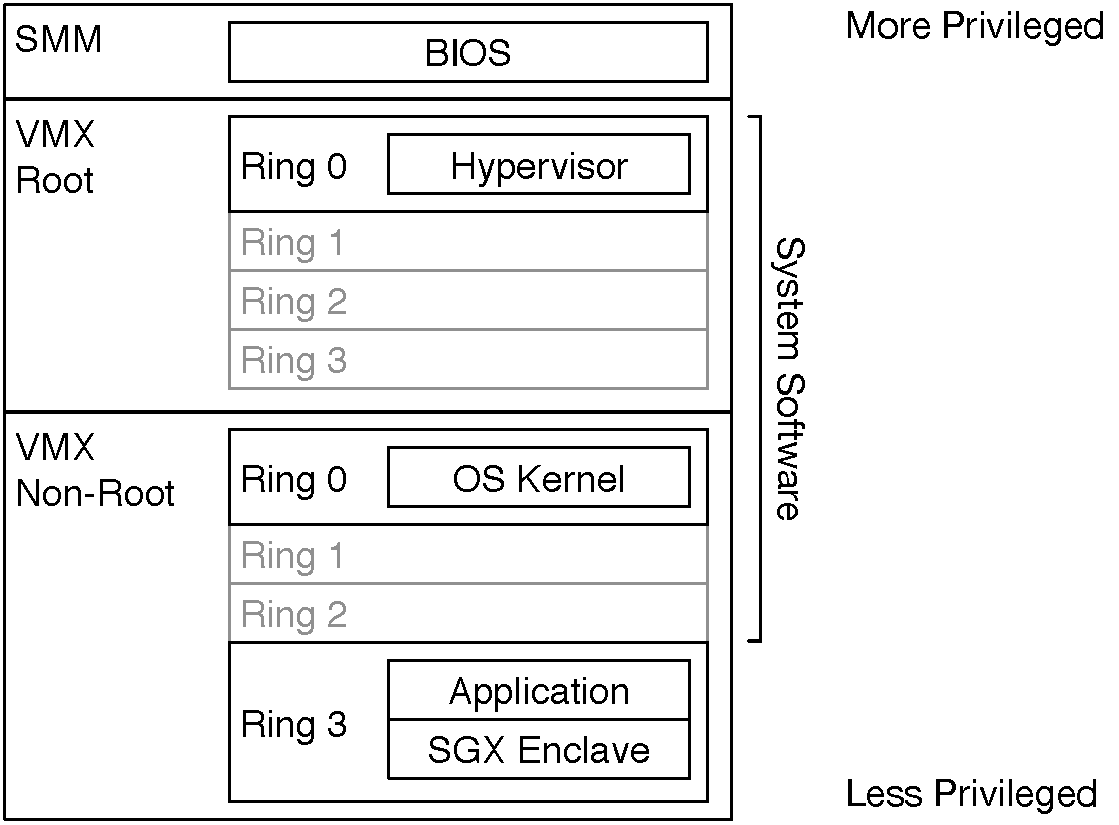
\includegraphics[width=75mm]{figures/cpu_rings.pdf}}
  \caption{
    Enclaves hold an application's private data and the code that operates on
    it. Therefore, they run at ring 3, in user mode.
  }
  \label{fig:computing_model}
\end{figure}


\section {SGX Analysis}

\subsection{SGX Implementation Overview}
\label{sec:sgx_implementation_overview}

An under-documented and overlooked feat achieved by the SGX design is that
implementing it on an Intel processor has a very low impact on the chip's
hardware design. SGX's modifications to the processor's execution
cores~(\S~\ref{sec:cpu_core}) are either very small or completely inexistent.
The CPU's uncore~(\S~\ref{sec:cpu_die}, \S~\ref{sec:cache_coherence}) receives
a new module, the  Memory Encryption Engine, which appears to be fairly
self-contained.

The bulk of the SGX implementation is relegated to the processor's
microcode~(\S~\ref{sec:microcode}), which supports a much higher development
speed than the chip's electrical circuitry.


\subsubsection{Execution Core Modifications}
\label{sec:sgx_core_modifications}

The SGX design may require a very small modification to the processor's
execution cores~(\S~\ref{sec:cpu_core}), in the Page Miss
Handler~(PMH,~\S~\ref{sec:tlbs}). The PMH resolves TLB misses, and consists of
a fast path that relies on an FSM page walker, and a microcode assist fallback
that handles the edge cases (\S~\ref{sec:microcode_pmh}).

The bulk of SGX's memory access checks, which are discussed in
\S~\ref{sec:sgx_access_protection}, can be implemented in the microcode assist.
The only modification to the PMH hardware is having it trigger the microcode
assist when the physical address produced by the page walker FSM matches the
Processor Reserved Memory~(PRM,~\S~\ref{sec:sgx_prm}) range.

We state that SGX \textbf{may} require a hardware modification to the PMH
because there is a possibility that the behavior described above can be
achieved solely with microcode configuration, as explained below.

The PRM range is configured by the PRM Range Registers~(\S~\ref{sec:sgx_prm}),
which have exactly the same semantics as the Memory Type Range
Registers~(MTRRs,~\S~\ref{sec:cacheability_config}) used to configure a
variable memory range. The page walker FSM in the PMH is already configured to
issue a microcode assist when the page tables are in uncacheable
memory~(\S~\ref{sec:memory_io}). Therefore, the PRMRR can be represented as an
extra MTRR pair.


\subsubsection{Uncore Modifications}
\label{sec:sgx_uncore_modifications}

The SDM states that DMA transactions~(\S~\ref{sec:motherboard}) that target the
PRM range are aborted by the processor. The SGX patents disclose that the PRMRR
protection aginst unauthorized DMA is implemented by having the SGX microcode
set up entries in the Source Address Decoder~(SAD) in the uncore CBoxes and in
the Target Address Decoder~(TAD) in the integrated Memory Controller~(MC).

\S~\ref{sec:cache_coherence} mentions that Intel's Trusted Execution
Technology~(TXT)~\cite{grawrock2009txt} already takes advantage of the
integrated MC to protect a DRAM range from DMA. It is highly likely that the
SGX implementation reuses the mechanisms brought by TXT, and only requires the
extension of the SADs and TADs by one entry.

SGX's major hardware modification is the Memory Encryption Engine~(MEE) that is
added to the processor's uncore~(\S~\ref{sec:cpu_die},
\S~\ref{sec:cache_coherence}) to protect SGX's Enclave Page
Cache~(EPC,~\S~\ref{sec:sgx_epc}) against physical attacks.

% ISCA SGX Slides 163-201

The MEE is briefly described in the ISCA 2015 SGX
tutorial~\cite{intel2015iscasgx}. According to the information presented there,
the MEE roughly follows the approach introduced by Aegis \cite{suh2003aegis}
\cite{aegis_impl}, which relies on a variation of Merkle trees to provide the
EPC with privacy, integrity, and freshness
guarantees~(\S~\ref{sec:crypto_primitives}). Unlike Aegis, the MEE uses
non-standard cryptographic primitives that include a slightly modified AES
operating mode~(\S~\ref{sec:privacy_crypto}) and a
Carter-Wegman~\cite{carter1977mac, wegman1981mac}
MAC~(\S~\ref{sec:integrity_crypto}) construction.

% ISCA SGX Slide 167

Both the ISCA SGX tutorial and the patents state that the MEE is connected to
to the Memory Controller (MC) integrated in the CPU's uncore. However, all
sources are completely silent on further implementation details. The
MEE overview slide states that ``the Memory Controller detects [the] address
belongs to the MEE region, and routes transaction to MEE'', which suggests that
the MEE is fairly self-contained and has a narrow interface to the rest of the
MC.


\subsubsection{Microcode Modifications}
\label{sec:sgx_microcode_modifications}

According to the SGX patents, all the SGX instructions are implemented in
microcode. This can also be deduced by reading the SDM's pseuodocode for all
the instructions, and realizing that it is highly unlikely that any SGX
instruction can be implemented in 4 or fewer
micro-ops~(\S~\ref{sec:out_of_order}), which is the most that can be
handled by the simple decoders used in the hardware fast paths
(S~\ref{sec:microcode_role}).

The Asynchronous Enclave Exit~(AEX,~\S~\ref{sec:sgx_aex}) behavior is also
implemented in microcode. \S~\ref{sec:microcode_structure} draws on an
assortment of Intel patents to conclude that hardware
exceptions~(\S~\ref{sec:faults}), including both faults and interrupts,
trigger microcode events~(\S~\ref{sec:microcode_structure}). It follows that
the SGX implementation can implement AEX by modifying the hardware exception
handlers in the microcode.

% ISCA SGX Slide 166

Last, the SGX initialization sequence is also implemented in microcode. It is
likely that the boot sequence in microcode~(\S~\ref{sec:microcode_sec}) was
modified to initialize the registers associated with the SGX microcode. The
ISCA SGX tutorial states that the MEE's keys are initialized during the boot
process.

% Intel SGX Opt-In Configuration: SDM S 37.7.1

The SDM states that SGX instructions are enabled by setting a bit in a
Model-Specific Register~(MSR,~\S~\ref{sec:address_spaces}). Initializing SGX
requires enabling the MEE and configuring the SAD and TAD to protect the PRM
range, and both tasks are amenable to a microcode implementation.

The SGX patents state that SGX requires very few hardware changes, and most of
the implementation is in microcode, as a positive fact. We therefore suspect
that minimizing hardware changes was a high priority in the SGX design, and
that any SGX modification proposals need to be aware of this priority.

\subsection{SGX Memory Access Protection}
\label{sec:sgx_access_protection}

SGX guarantees that the software inside an enclave is isolated from all the
software outside the enclave, including the software running in other enclaves.
This isolation guarantee is at the core of SGX's security model.

It is tempting to assume that the main protection mechanism in SGX is the
Memory Encryption Engine (MEE) described in
\S~\ref{sec:sgx_uncore_modifications}, as it encrypts and MACs the DRAM's
contents. However, the MEE sits in the processor's memory controller, which is
at the edge of the on-chip memory hierarchy, below the
caches~(\S~\ref{sec:caching}). Therefore, the MEE cannot protect an enclave's
memory from software attacks.

% Page-Based Access Control: SDM S 38.5
% Interactions with Paging: SDM S 42.4
% ISCA SGX Slide 27

The root of SGX's protections against software attacks is a series of memory
access checks which prevents the currently running software from accessing
memory that does not belong to it. Specifically, non-enclave software is only
allowed to access memory outside the PRM range, while the code inside an
enclave is allowed to access non-PRM memory, and the EPC pages owned by the
enclave.

Although it is believed~\cite{evtyushkin2014isox} that SGX's access checks are
performed on every memory access checks, all our information sources indicate
that the access checks are only performed during TLB misses. The intuition
behind this finding can be built by considering what it would take to implement
SGX's memory access protections in a trusted operating system or hypervisor,
solely by using the page tables that direct the CPU's address
translation feature~(\S~\ref{sec:paging}).

The hypothetical trusted software described above can implement enclave
entry~(\S~\ref{sec:sgx_eenter}) would be implemented as a system
call~\S~\ref{sec:syscalls} that creates page table entries mapping the
enclave's memory. Enclave exit~(\S~\ref{sec:sgx_eexit}) can be a symmetric
system call that removes the page table entries created during enclave entry.
When modifying the page tables, the system software has to consider TLB
coherence issues~(\S~\ref{sec:tlbs}) and perform TLB shootdowns when
appropriate.

SGX leaves page table management under the system software's control, but it
cannot trust the software to set up the page tables in any particular way.
Therefore, the hypothetical design described above cannot be used by SGX as-is.
Instead, at a conceptual level, the SGX implementation approximates the effect
of having the page tables set up correctly by inspecting every address
translation that comes out of the Page Miss Handler~(PMH,~\S~\ref{sec:tlbs}).
The address translations that do not obey SGX's access control restrictions
are rejected before they have a chance to reach the TLBs and be used to service
load and store instructions.

% Enclave Page Cache Map (EPCM): SDM S 37.5.1, SDM S 38.19
% Security Information (SECINFO): SDM S 38.11, S 38.11.{1,2}
% SECINFO.FLAGS: SDM S 38.11.1
% PAGE_TYPE Field Definition: SDM S 38.11.2

The SGX address translation checks use the information in the Enclave Page
Cache Map~(EPCM,~\S~\ref{sec:sgx_epcm}), which is effectively an inverted page
table that covers the entire EPC. This means that each EPC page is accounted
for by an EPCM entry, using the structure is summarized in
Table~\ref{fig:sgx_epcm_entry}. The EPCM fields were described in detail in
\S~\ref{sec:sgx_epcm}, \S~\ref{sec:sgx_paging}, \S~\ref{sec:sgx_tcs},
\S~\ref{sec:sgx_eblock}, and \S~\ref{sec:sgx_va}.

\begin{table}[hbt]
  \centering
  \begin{tabularx}{\columnwidth}{| l | r | X |}
  \hline
  \textbf{Field} & \textbf{Bits} & \textbf{Description}\\
  \hline
  VALID & 1 & 0 for un-allocated EPC pages \\
  \hline
  BLOCKED & 1 & page is being evicted \\
  \hline
  R & 1 & enclave code can read \\
  \hline
  W & 1 & enclave code can write \\
  \hline
  X & 1 & enclave code can execute \\
  \hline
  PT & 8 & page type (Table~\ref{fig:sgx_pt_values}) \\
  \hline
  ADDRESS & 48 & the virtual address used to access this page \\
  \hline
  ENCLAVESECS & 52 & the physical address of the SECS of the enclave owning the
                     page \\
  \hline
  \end{tabularx}
  \caption{
    The fields in an EPCM entry.
  }
  \label{fig:sgx_epcm_entry}
\end{table}

\begin{table}[hbt]
  \centering
  \begin{tabularx}{\columnwidth}{| l | l | X |}
  \hline
  \textbf{Type} & \textbf{Allocated by} & \textbf{Contents}\\
  \hline
  PT\_REG & \texttt{EADD} & enclave code and data \\
  \hline
  PT\_SECS & \texttt{ECREATE} & SECS (\S~\ref{sec:sgx_secs}) \\
  \hline
  PT\_TCS & \texttt{EADD} & TCS (\S~\ref{sec:sgx_tcs}) \\
  \hline
  PT\_VA & \texttt{EPA} & VA (\S~\ref{sec:sgx_va}) \\
  \hline
  \end{tabularx}
  \caption{Values of the PT (page type) field in an EPCM entry.}
  \label{fig:sgx_pt_values}
\end{table}

SGX's extensions to the PMH spring into life every time when the physical
address produced by the page walker FSM falls into the PRM range, and perform
the security checks illustrated in Figure~\ref{fig:sgx_tlb_miss_checks}.

\begin{figure}[hbt]
  \centering
  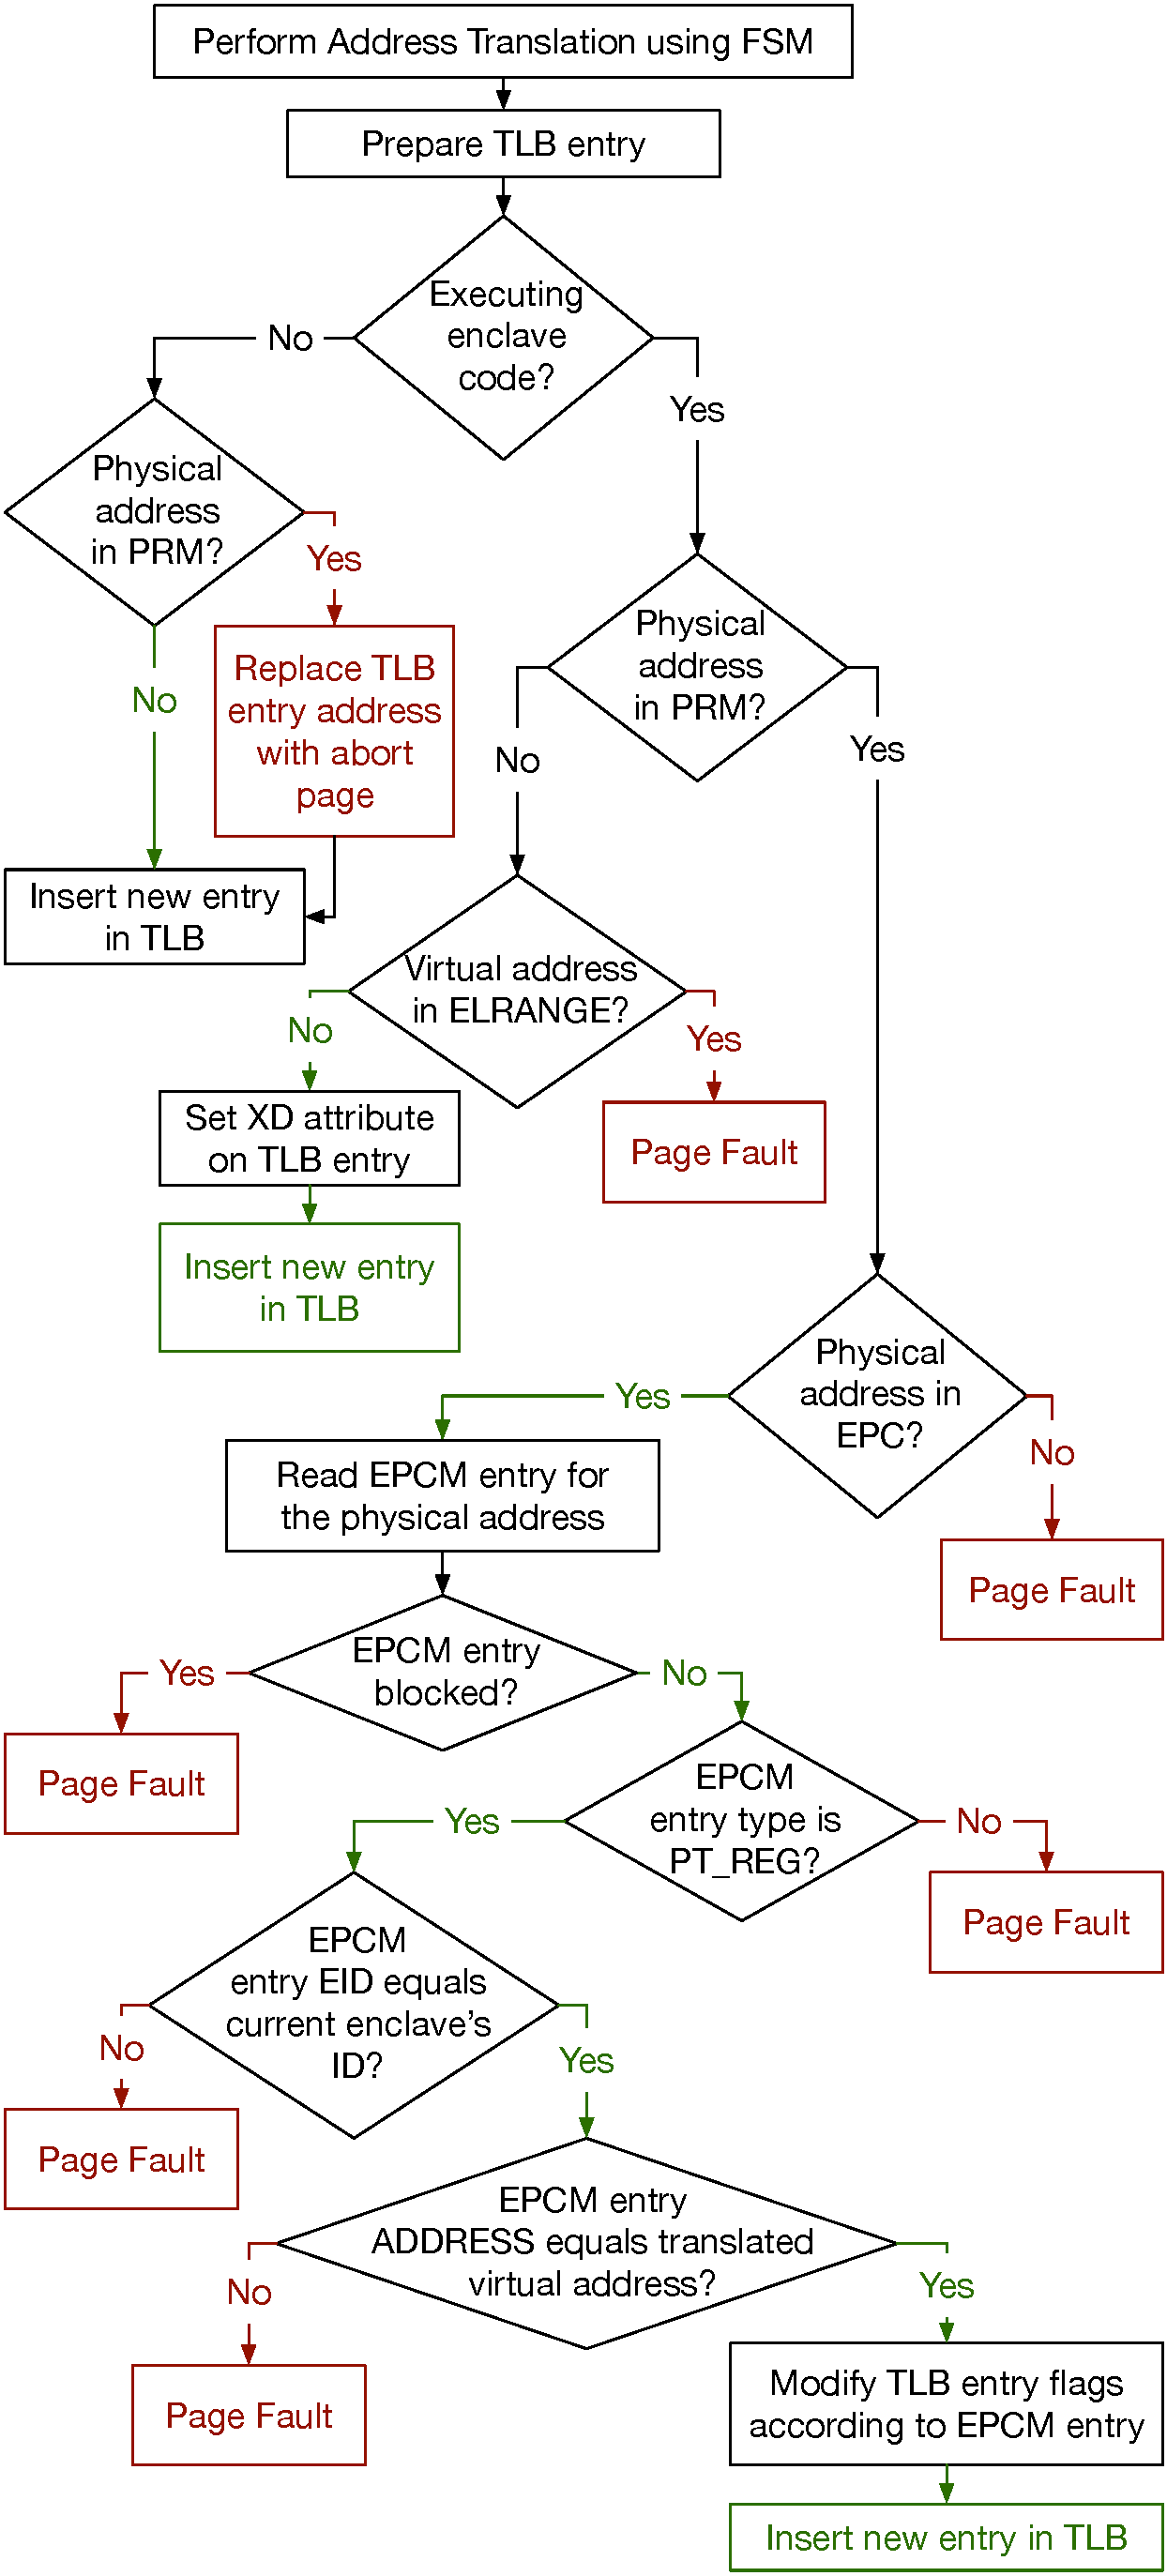
\includegraphics[width=85mm]{figures/sgx_tlb_miss_checks.pdf}
  \caption{
    The access control logic added by SGX to the PMH
  }
  \label{fig:sgx_tlb_miss_checks}
\end{figure}

The EPCM is inspected every time when
translation result is the physical
address of an EPC page, the CPU ensures\footnote{A mismatch triggers a general
protection fault (\#GP, \S~\ref{sec:faults}).} that the virtual address given
to the address translation process matches the expected virtual address
recorded in the page's EPCM entry, as shown in
Figure~\ref{fig:sgx_tlb_miss_checks}. This prevents the system software, which
manages the page tables and EPT, from modifying an enclave's virtual address
space in a manner that is inconsistent with the enclave author's expectations.


SGX's security revolves around maintaining the following
invariant. \textbf{At all times, a logical processor's TLB
entries can only map DRAM pages that can be accessed by the code executing on
the processor.} Specifically, when a logical processor is in enclave mode, its
TLB can include entries for the enclave's EPC pages, and for DRAM pages outside
the PRM. The TLB of a logical processor outside enclave mode must not include
any PRM entry.

Without any special measures, the invariant described above would be broken
when a logical processor exits an enclave, either via
\texttt{EEXIT}~(\S~\ref{sec:sgx_eexit}), or via an AEX~(\S~\ref{sec:sgx_aex}).
This is because enclave mode allows TLB entries that point to the currently
executing enclave's EPC pages, and these entries become disallowed the moment
the processor leaves enclave mode. The SGX implementation solves this problem
by flushing a logical processor's TLBs when it leaves enclave mode.

\HeadingLevelB{Enclave Signature Verification}
\label{sec:sgx_rsa_check}

Let $m$ be the public modulus in the enclave author's RSA key, and $s$ be the
enclave signature. Since the SGX design fixes the value of the public exponent
$e$ to $3$, verifying the RSA signature amounts to computing the signed
message $M = s^3 \bmod m$, checking that the value meets the PKCS v1.5 padding
requirements, and comparing the 256-bit SHA-2 hash inside the message with the
value obtained by hashing the relevant fields in the SIGSTRUCT supplied with
the enclave.

This section describes an algorithm for computing the signed message while only
using subtraction and multiplication on large non-negative integers. The
algorithm admits a significantly simpler implementation than the typical RSA
signature verification algorithm, by avoiding the use of long division and
negative numbers. The description here is essentially the idea in
\cite{gueron2011rsasig}, specialized for $e = 3$.


The algorithm provided here requires the signer to compute the $q_1$ and
$q_2$ values shown below. The values can be computed from the public
information in the signature, so they do not leak any additional information
about the private signing key. Furthermore, the algorithm verifies the
correctness of the values, so it does not open up the possibility for an attack
that relies on supplying incorrect values for $q_1$ and $q_2$.

\begin{align*}
q_1 & = \left\lfloor \frac{s^2}{m} \right\rfloor \\
q_2 & = \left\lfloor \frac{s^3 - q_1 \times s \times m}{m} \right\rfloor
\end{align*}

Due to the desirable properties mentioned above, it is very likely that the
algorithm described here is used by the SGX implementation to verify the RSA
signature in an enclave's SIGSTRUCT~(\S~\ref{sec:sgx_sigstruct}).

The algorithm in Figure~\ref{fig:sgx_sig_verification} computes the signed
message $M = s^3 \bmod m$, while also verifying that the given values of $q_1$
and $q_2$ are correct. The latter is necessary because the SGX implementation
of signature verification must handle the case where an attacker attempts to
exploit the signature verification implementation by supplying invalid values
for $q_1$ and $q_2$.

\begin{figure}[hbt]
  \begin{enumerate}
    \item Compute $u \leftarrow s \times s$ and $v \leftarrow q_1 \times m$
    \item If $u < v$, abort. $q_1$ must be incorrect.
    \item Compute $w \leftarrow u - v$
    \item If $w \ge m$, abort. $q_1$ must be incorrect.
    \item Compute $x \leftarrow w \times s$ and $y \leftarrow q_2 \times m$
    \item If $x < y$, abort. $q_2$ must be incorrect.
    \item Compute $z \leftarrow x - y$.
    \item If $z \ge m$, abort. $q_2$ must be incorrect.
    \item Output $z$.
  \end{enumerate}
  \caption{
    An RSA signature verification algorithm specialized for the case where
    the public exponent is 3. $s$ is the RSA signature and $m$ is the RSA key
    modulus. The algorithm uses two additional inputs, $q_1$ and $q_2$.
  }
  \label{fig:sgx_sig_verification}
\end{figure}

The rest of this section proves the correctness of the algorithm in
Figure~\ref{fig:sgx_sig_verification}.


\HeadingLevelC{Analysis of Steps 1 - 4}

Steps $1 - 4$ in the algorithm check the correctness of $q_1$ and use it
to compute $s^2 \bmod m$. The key observation to understanding these steps is
recognizing that $q_1$ is the quotient of the integer division $s^2 / m$.

Having made this observation, we can use elementary division properties to
prove that the supplied value for $q_1$ is correct if and only if the following
property holds.

$$ 0 \le s^2 - q_1 \times m < m $$

We observe that the first comparison, $0 \le s^2 - q_1 \times m$, is equivalent
to $q_1 \times m \le s^2$, which is precisely the check performed by step 2. We
can also see that the second comparison, $s^2 - q_1 \times m < m$ corresponds
to the condition verified by step 4. Therefore, if the algorithm passes step 4,
it must be the case that the value supplied for $q_1$ is correct.

We can also plug $s^2$, $q_1$ and $m$ into the integer division remainder
definition to obtain the identity $s^2 \bmod m = s^2 - q_1 \times m$. However,
according to the computations performed in steps 1 and 3,
$w = s^2 - q_1 \times m$. Therefore, we can conclude that $w = s^2 \bmod m$.


\HeadingLevelC{Analysis of Steps 5 - 8}

Similarly, steps $5 - 8$ in the algorithm check the correctness of $q_2$ and
use it to compute $w \times s \bmod m$. The key observation here is that
$q_2$ is the quotient of the integer division $(w \times s) / m$.

We can convince ourselves of the truth of this observation by using the fact
that $w = s^2 \bmod m$, which was proven above, by plugging in the definition
of the remainder in integer division, and by taking advantage of the
distributivity of integer multiplication with respect to addition.

\begin{align*}
\left\lfloor \frac{w \times s}{m} \right\rfloor
    & = \left\lfloor \frac{(s^2 \bmod m) \times s}{m} \right\rfloor \\
    & = \left\lfloor \frac{(s^2 - \lfloor \frac{s^2}{m} \rfloor \times m)
        \times s}{m} \right\rfloor \\
    & = \left\lfloor \frac{s^3 - \lfloor \frac{s^2}{m} \rfloor \times m
        \times s}{m} \right\rfloor \\
    & = \left\lfloor \frac{s^3 - q_1 \times m \times s}{m} \right\rfloor \\
    & = \left\lfloor \frac{s^3 - q_1 \times s \times m}{m} \right\rfloor \\
    & = q_2
\end{align*}

By the same argument used to analyze steps $1 - 4$, we use elementary division
properties to prove that $q_2$ is correct if and only if the equation below is
correct.

$$ 0 \le w \times s - q_2 \times m < m $$

The equation's first comparison, $0 \le w \times s - q_2 \times m$, is
equivalent to $q_2 \times m \le w \times s$, which corresponds to the check
performed by step 6. The second comparison, $w \times s - q_2 \times m < m$,
matches the condition verified by step 8. It follows that, if the algorithm
passes step 8, it must be the case that the value supplied for $q_2$ is
correct.

By plugging $w \times s$, $q_2$ and $m$ into the integer division remainder
definition, we obtain the identity
$w \times s \bmod m = w \times s - q_2 \times m$. Trivial substitution reveals
that the computations in steps 5 and 7 result in
$z = w \times s - q_2 \times m$, which allows us to conclude that
$z = w \times s \bmod m$.

In the analysis for steps $1 - 4$, we have proven that $w = s ^ 2 \bmod m$. By
substituting this into the above identity, we obtain the proof that the
algorithm's output is indeed the desired signed message.

\begin{align*}
z & = w \times s \bmod m \\
  & = (s^2 \bmod m) \times s \bmod m \\
  & = s^2 \times s \bmod m \\
  & = s^3 \bmod m
\end{align*}


\HeadingLevelC{Implementation Requirements}

The main advantage of the algorithm in Figure~\ref{fig:sgx_sig_verification} is
that it relies on the implementation of very few arithmetic operations on large
integers. The maximum integer size that needs to be handled is twice the size
of the modulus in the RSA key used to generate the signature.

Steps 1 and 5 use large integer multiplication. Steps 3 and 7 use integer
subtraction. Steps 2, 4, 6, and 8 use large integer comparison. The checks in
steps 2 and 6 guarantee that the results of the subtractions performed in steps
3 and 7 will be non-negative. It follows that the algorithm will never
encounter negative numbers.

\section{The Hardware Underpinnings of SGX}

The security of SGX hinges on the assumption that it is very difficult for an
attacker to produce an attestation that contains attacker-supplied information
in the enclave field. In order to evaluate this claim, we must understand the
hardware protection mechanisms and the encryption schemes involved in the
process.

Most of the material in this section comes from Intel's
patents~\cite{intel2013patent1, intel2013patent2}, because the SGX papers and
reference consider this information an implementation detail. We point out when
a piece of information matches the SGX manual or one of the SGX papers.

According to the Intel patents, the SGX instructions are implemented in
microcode. The statement in \cite{anati2013sgx} that a microcode update changes
the platform TCB confirms this finding. The patents state that SGX requires
very few hardware changes, and most of the implementation is in microcode, as a
positive fact, fueling our suspicion that minimizing hardware changes was a
high priority in the SGX design.


\subsection{Memory Protection Mechanisms}

The SGX reference manual states that the Processor Reserved Memory (PRM) is
allocated by the BIOS, by setting the PRM range registers (PRMRR). The patents
refer to this range as the secure enclave range registers (SERR), and state
that the memory range is protected from DMA accesses by a dedicated pair of
SAD / TAD entries (\S~\ref{sec:cpu_uncore}).
The patents state that the SAD and TAD entries mirror the PRMRR registers
which, if done correctly, does prevent against DMA snooping.

The SGX reference manual states that the EPC memory is protected against
physical snooping attacks on the DRAM by an implementation-dependent mechanism,
and suggests that the most likely implementation is a Memory Encryption Engine
(MEE). The MEE is called a crypto engine in the Intel patents, which state that
the crypto engine is connected to the QuickPath Interconnect (QPI) home agent
in each processor, and it encrypts all RAM accesses in a range called the
Crypto Memory Aperture (CMA), before they reach the memory controller. The CMA
range is configured by setting the Crypto Memory Range Registers (CMRR). The
CMA contains the EPC, EPCM, and other data structured used by the SGX
implementations, which leads us to believe that the CMA covers the entire PRM
range, and the CMRR and PRMRR are identical. One of the SGX
papers~\cite{mckeen2013sgx} states that the PRM may be covered by one or more
MEE regions.

The data inside the CMA is lost when the CPU is powered down (including when it
enters the S3 power management state), so enclaves must be either torn down by
the OS, or their EPC pages must be evicted to RAM, and eventually to disk.

The EPC encryption described above is only intended to defend against physical
attacks. Enclaves are isolated from system software (the OS and hypervisor) by
access control checks in the CPU, as described in \S~\ref{sec:epcm}. The
patents specify the protection algorithm with more clarity.

The patents also specify that the memory access checks are performed in the
Page-Miss Handler (PMH) microcode, which is invoked during TLB misses. The PMH
performs the SGX access checks described below. If the access checks succeed,
the PMH creates a TLB entry, as it normally would. If the access checks fail,
the PMH aborts, which results in a Page Fault. The desire to restrict SGX
access checks to the PMH introduces the requirement to flush a logical
processor's TLBs when it enters or exits enclave mode. This is accomplished by
adding 1 bit to TLB entries, which differentiates between enclave pages and
non-enclave pages.
On enclave entry and exit, all the TLB entries that have the enclave bit set
are flushed. One of the SGX papers~\cite{mckeen2013sgx} confirms that the EPCM
is checked by the PMH.
The SGX manual also confirms this: ``The Intel SGX access control itself is
implemented as an extension to the traditional IA-32 paging/EPT state
machine.''
The Intel patents state that future implementations may optimize away the TLB
flushes by adding enclave ID tags to TLB entries.

The SGX access checks occur after the normal page address translation process
(described in the Intel SDM) completes.
If the resulting physical address does not fall within the CMA, the
SGX access checks do not apply.
A CMA memory access is only allowed if originates from the CPU's microcode
(used to implement the SGX instructions), or if it an admissible enclave
access.
The latter is true if the logical processor making the memory access is in
enclave mode, the accessed physical address falls in an EPC range, the page's
EPCM entry has the present (P) bit set and does not have the blocked (B) bit
set, the current enclave's ID matches the enclave ID in the page's EPCM entry,
and the linear address used to access the page matches the one in the page's
EPCM entry.

The Intel patents call ELRANGE the Enclave Linear Space (ELS) range.



\subsection{Key Hierarchy and Derivation}

According to Intel's patents, the SGX implementation relies on a complex key
derivation process rooted on global secret keys in the CPU circuitry, and on
secrets embedded in the processor's eFUSEs. eFUSE information can be extracted
efficiently (Chipworks quoted us \$50-250k for extracting the entire eFUSE
contents from an Intel i5 processor), so some of the eFUSE secrets are
encrypted with a master key (referred to as a ``global wrapping logic key'' in
the patents).

The patents state that encrypting the eFUSE secrets by the logic key makes them
harder to extract via hardware monitoring tools, and protects them while in
transit to the CPU during the manufacturing process. This assumes that it is
very expensive to obtain the global key from a CPU, by virtue of the low
feature size.

The SGX patents describe two ``logic keys'' embedded in the CPU's circuitry,
which are the same for all CPUs in a stepping, making them essentially global
keys. The \textit{global wrapping logic key} is a 128-bit AES key, and it is
used to encrypt a subset a 256-bit A.x value used to re-create the CPU's EPID
key, and a 128-bit \textit{pre-seed key 0}. The eFUSEs also contain a 128-bit
\textit{pre-seed key 1} and a 32-bit EPID group ID, which are stored in
cleartext.

The SGX manuals~\cite{intel2013sgxmanual, intel2014sgx2manual} mention a
16-byte CPU security version number (SVN), which contains the version numbers
of various TCB components, and is a source in the key derivation process. The
patents further specify that the SVN register is made up of (most likely 8-bit)
sections that contain the SVNs of each layer in the SGX initialization process,
and that each initialization step sets the corresponding section to its SVN,
and then locks it for the duration of the power-up cycle.

Intel's patents disclose that the key derivation process uses 128-bit AES in
ECB mode as a pseudo-random function (PRF). When an SVN is an input to a key
derivation process, a \textit{PRF loop} is used, where the PRF is applied to
a constant



\cite{anati2013sgx} confirms that the attestation uses Intel's
EPID~\cite{brickell2009epid} group signature scheme.


Key Request Inputs

\begin{table}[hbt]
  \center{\begin{tabularx}{\columnwidth}{| l | l | X |}
  \hline
  \textbf{Name} & \textbf{Size} & \textbf{Description}\\
  \hline
  Key Name & 2 & Which key will be derived \\
  \hline
  Policy & 2 & Whether the key derivation uses MRENCLAVE or MRSIGNER \\
  \hline
  ISV SVN & 2 & Developer-assigned SVN \\
  \hline
  CPU SVN & 16 & 128-bit TCB SVN \\
  \hline
  KeyID & 32 & Used for wear-out protection \\
  \hline
  Attribute Mask & 16 & Which SECS ATTRIBUTES are used in Seal Key \\
  \hline
  MISC Mask & 2 & Which SECS MISCSELECT bits are used in Seal Key \\
  \hline
  \end{tabularx}}
  \caption{Values of the PT (page type) field in an EPCM entry.}
  \label{fig:key_request_inputs}
\end{table}

Key names: LAUNCH, PROVISION, PROVISION\_SEAL, REPORT, SEAL.


\subsection{Data Structures}

The Intel patents state that the 128-bit enclave key is stored in the enclave's
SECS page, and that SGX security depends on enclaves not being able to read
their own SECS pages. They also state that the enclave key is used to encrypt
the EPC pages when they are evicted to untrusted RAM. The patents also state
that the enclave's SECS page contains the SVN of the launch permit creator.

The Intel patents state that each TCS has two fields that store the values of
the DR7 and IA32\_DEBUGCTL registers during EENTER, and are used to restore the
original values during EEXIT and AEX.

The Intel patents state that the enclave ID used in EPCM entries is the
phyisical address of the page holding the enclave's SECS, without the bottom
12 bits that are guaranteed to be zero. The SGX manual indicates that when an
EPC page is allocated via EADD, the physical address of its enclave's SECS is
cached, until the page is removed via EREMOVE. This, together with the fact
that the enclave ID's location in the SECS is not specified, indicates that the
enclave's ID is indeed the physical address of its SECS page.


The Intel patents indicate that EREPORT's KeyID is initialized to a random
value on each processor power cycle, and is incremented after $2^{32}$ AES
operations that use the value. They also indicate that each EREPORT may
increment the KeyID by 1.



\section{SGX Memory Organization}
\label{sec:memory}

The central concept of SGX is the \textit{enclave}, a protected environment
that contains the code and data pertaining to a security-sensitive computation.
This section provides an overview of the data structures used by an enclave.


\subsection{Enclaves in DRAM}
\label{sec:prm}

% Intel SGX Resource Enumeration Leaves: SDM S 37.7.2
% Interactions with DMA: SDM S 42.10, SGX2 S 6.10

The enclaves' code and data is stored in \textit{Processor Reserved Memory}
(PRM), which cannot be directly accessed by other software, including system
software and SMM code. The CPU's integrated memory controllers
(\S~\ref{sec:cpu_die}) also reject DMA transfers targeting the PRM, thus
protecting it from access by other peripherals.

\begin{figure}[hbt]
  \centering
  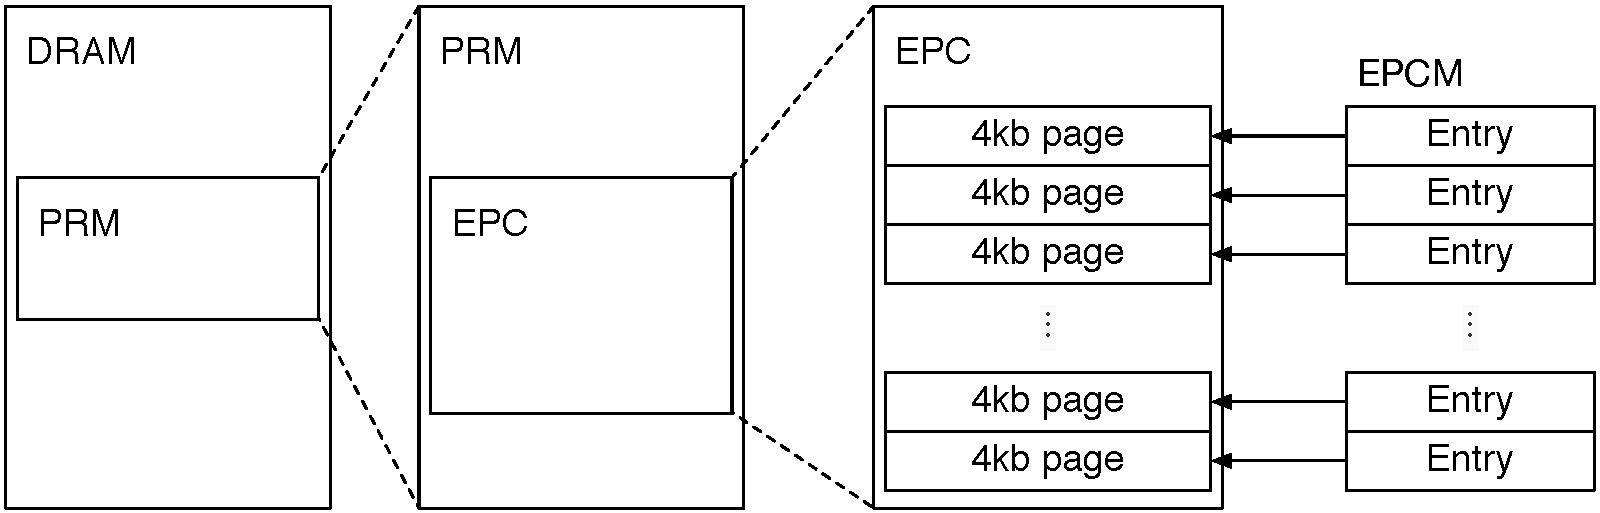
\includegraphics[width=87mm]{figures/sgx_epc.pdf}
  \caption{
    Enclave data is stored into the EPC, which is a subset of the PRM. The
    PRM is a contiguous range of DRAM that cannot be accessed by system
    software or peripherals.
  }
  \label{fig:sgx_epc}
\end{figure}

% EPC and Management of EPC Pages: SGX2 S 3.5
% Interactions with Memory Configuration: SGX2 S 6.11
% Memory Type Considerations for PRMRR: SGX2 S 6.11.1
% Interactions of PRMRR with Physical Memory Accesses: SGX2 S 6.11.3.1

The PRM range is configured using a base and a mask register with the same
semantics as a variable memory type range (\S~\ref{sec:cacheability_config}),
which implies that the PRM's size must be an integer power of two, and its
start address must be aligned to the same power of two. These restrictions make
it cheap to check if an address belongs to the PRM in hardware, as described in
\S~\ref{sec:cacheability_config}.

The PRM and PRM range registers (PRMRR) are described in the SGX
manuals~\cite{intel2013sgxmanual, intel2014sgx2manual} and in one of the SGX
papers~\cite{mckeen2013sgx}. The SDM mostly mirrors the SGX manuals, but lacks
most of the sections mentioning the PRM.


\subsubsection{The Enclave Page Cache (EPC)}
\label{sec:epc}

% Enclave Page Cache: SDM S 37.5
% EPC and Management of EPC Pages: SDM S 39.5, S 39.5.1

The contents of enclaves and the associated data structures are stored in the
\textit{Enclave Page Cache} (EPC), which is a subset of the PRM.

The SGX design supports having multiple enclaves on a system at the same time,
which is a  necessity in multi-process environments. This is achieved by having
the EPC split into 4~KB pages that can be associated to different enclaves. The
system software uses SGX instructions to allocate unused pages to enclaves, and
to free previously allocated EPC pages.

The SGX instructions that allocate an EPC page to an enclave also copy data
from a page outside PRM to the EPC page. Non-enclave software is not permitted
to access the PRM, so the page allocation instructions are the only avenue for
system software to load the initial code and data into an enclave.

SGX also offers a method for system software to evict EPC pages into non-PRM
memory, which allows the EPC to be over-committed, just like evicting DRAM
pages to disk (swapping) allows the main memory to be over-committed.


\subsubsection{Memory Mapping Attacks}
\label{sec:mapping_attacks}

% Access Control Requirements: SDM S 38.3

One of SGX's design goals is to make it easy to migrate the sensitive pieces of
an application into an enclave. To this end, enclave code uses the same address
translation process (\S~\ref{sec:paging}) as the application hosting the
enclave. It follows that enclave code can access non-EPC memory using the same
virtual addresses as the host application, which makes it easy to migrate
application code that uses pointers into SGX enclaves.

% Interactions with VMX: SDM S 42.5, S 42.5.{1,2,3,4,5}

Under SGX, the operating system and hypervisor are still in full control of the
page tables and EPTs. This minimizes the amount of changes required to add SGX
support to existing system software. However, it also gives system software the
ability to attack an enclave by setting up its virtual address space in a way
that was not intended by the enclave's author.

Figure~\ref{fig:sgx_mapping_attack} shows a hypothetical memory mapping attack
that is prevented by SGX's security measures. Understanding this type of attack
greatly increases one's ability to reason about SGX's security.

\begin{figure}[hbt]
  \centering
  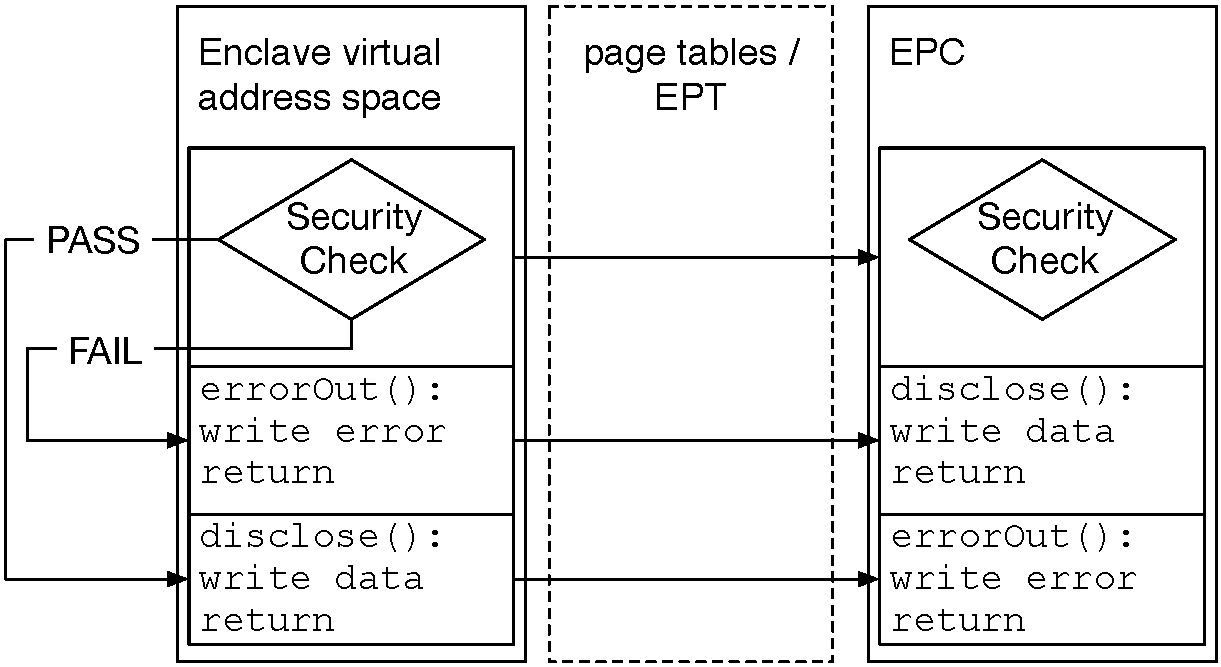
\includegraphics[width=85mm]{figures/sgx_mapping_attack.pdf}
  \caption{
    An example of a memory mapping attack, which is prevented by SGX. The
    enclave's author intends to disclose a piece of sensitive information only
    when a security check passes. Malicious system software maps the virtual
    address of the procedure called when the security check fails to an EPC
    page that contains the procedure that discloses the sensitive information,
    which is supposed to be called when the security check passes.
  }
  \label{fig:sgx_mapping_attack}
\end{figure}

For simplicity, we assume an enclave that performs a security check to decide
whether to disclose some sensitive information. Depending on the security
check's outcome, the enclave code either calls a \texttt{errorOut} procedure,
or a \texttt{disclose} procedure. We furthermore assume that each procedure's
code starts at a 4KB boundary, and takes up less than 4KB, so each procedure
fits in an EPC page. These requirements seem unrealistic, but the underlying
attack remains an issue in real applications.

In a memory mapping attack, malicious system software sets up the page tables
or EPT in such a way that the virtual address intended to store the
\texttt{errorOut} procedure is actually mapped to an EPC page that contains the
\texttt{disclose} procedure. Without any security measures in place, the
enclave would execute the \texttt{disclose} code and reveal sensitive
information, even though the security check fails.

The SGX security mechanisms, explained throughout the rest of this paper,
prevent enclave code execution if a memory mapping attack occurs. Therefore,
SGX prevents malicious system software from directly obtaining sensitive
information via memory mapping attacks.


\subsubsection{The Enclave Page Cache Map (EPCM)}
\label{sec:epcm}

% Enclave Page Cache Map (EPCM): SDM S 37.5.1, SDM S 38.19
% SECINFO.FLAGS: SDM S 38.11.1
% PAGE_TYPE Field Definition: SDM S 38.11.2

SGX prevents memory mapping attacks using the \textit{Enclave Page Cache Map}
(EPCM), which has an entry for each EPC page, containing the security metadata
shown in Table~\ref{fig:epcm_entry}.

\begin{table}[hbt]
  \centering
  \begin{tabularx}{\columnwidth}{| l | r | X |}
  \hline
  \textbf{Field} & \textbf{Bits} & \textbf{Description}\\
  \hline
  VALID & 1 & 0 for un-allocated EPC pages \\
  \hline
  BLOCKED & 1 & page is being evicted (\S~\ref{sec:sgx_ewb})\\
  \hline
  R & 1 & allow reads by enclave code\\
  \hline
  W & 1 & allow writes by enclave code\\
  \hline
  X & 1 & allow execution of code inside the page, inside enclave\\
  \hline
  PT & 8 & page type (\S~\ref{sec:key_structures})\\
  \hline
  ADDRESS & 48 & the virtual address used to access this page\\
  \hline
  EID & 64 & identifies the enclave owning the page\\
  \hline
  \end{tabularx}
  \caption{
    The fields in an EPCM entry.
  }
  \label{fig:epcm_entry}
\end{table}

% Access Control Requirements: SDM S 38.3

SGX's main weapon against memory mapping attacks is the ENCLAVEADDRESS metadata
field, which contains the expected virtual address (\S~\ref{sec:segments}) used
to access the page. The expected virtual address must be specified when a page
is allocated, and cannot be changed until the page is freed.

When an address translation (\S~\ref{sec:paging}) result is the physical
address of an EPC page, the CPU ensures\footnote{A mismatch triggers a general
protection fault (\#GP, \S~\ref{sec:faults}).} that the virtual address given
to the address translation process matches the expected virtual address
recorded in the page's EPCM entry.  This prevents the system software, which
manages the page tables and EPT, from modifying an enclave's virtual address
space in a manner that is inconsistent with the enclave author's expectations.

% Security Information (SECINFO): SDM S 38.11, S 38.11.{1,2}

The EPCM entry for a page has three access protection bits that must be set to
1 to allow a page to be read (R), written to (W) and executed (X) by enclave
code. When an address translation result points to an EPC page, the access
protection bits in the page's EPCM entry influence the related bits in the
page's TLB entry. For example, if X is 0, the XD bit (\S~\ref{sec:paging}) is
set in the page's TLB entry.

The EPCM also stores the ID of the enclave that owns each EPC page, so the
processor can prevent the code inside an enclave from accessing pages that
belong to other enclaves.

A page's EPCM entry also records a \textit{page type} (PT) for each page.
Table~\ref{fig:pt_values} shows currently defined types. The EPC pages that
store an enclave's code or data have their type set to \textit{regular}
(PT\_REG in the Intel documentation). Each page that is dedicated to an SGX key
data structure has its EPCM entry's type set to the kind of data structure
stored in the page. An EPC page's type is set when the page is allocated, and
is immutable throughout the page's lifetime.

\begin{table}[hbt]
  \centering
  \begin{tabularx}{\columnwidth}{| l | l | X |}
  \hline
  \textbf{Type} & \textbf{Created by} & \textbf{Description}\\
  \hline
  PT\_REG & \texttt{EADD} & enclave code / data \\
  \hline
  PT\_SECS & \texttt{ECREATE} & SECS (\S~\ref{sec:secs}) \\
  \hline
  PT\_TCS & \texttt{EADD} & TCS (\S~\ref{sec:tcs}) \\
  \hline
  PT\_VA & \texttt{EPT} & VA (\S~\ref{sec:va}) \\
  \hline
  \end{tabularx}
  \caption{Values of the PT (page type) field in an EPCM entry.}
  \label{fig:pt_values}
\end{table}

The SGX documentation does not state where the EPCM is stored, but guarantees
that the EPCM is ``trusted memory''. The documentation also does not describe
the EPCM layout.


\subsection{Key SGX Structures}
\label{sec:key_structures}

% Access Control Requirements: SDM S 38.3

Pages that store key SGX structures cannot be accessed directly, even by the
code executing inside their enclaves. Furthermore, the SGX instructions that
operate on SGX data structures check the EPCM type fields of their inputs
against the expected types. This type system prevents software from
intentionally or accidentally corrupting the key SGX data structures.

The type-based access restrictions have the desirable side-effect of hiding the
contents of the EPC pages holding key SGX structures from software, so the
internal layout of any key data structure can change across new CPU revisions.
Software cannot access the key structures in EPC, so it cannot become dependent
on a specific processor's implementation details. This is a stronger version of
the encapsulation used in the Virtual Machine Constrol Structure
(VMCS, \S~\ref{sec:vmx}).

The SGX documentation does specify a software-visible layout for each key data
structure. This layout is used by the non-EPC page used to initialize the key
data structure when it is created. Therefore, new CPU revisions must preserve
the ability to initialize the key data structures from the less flexible
software-visible layout.

\begin{figure}[hbt!]
  \centering
  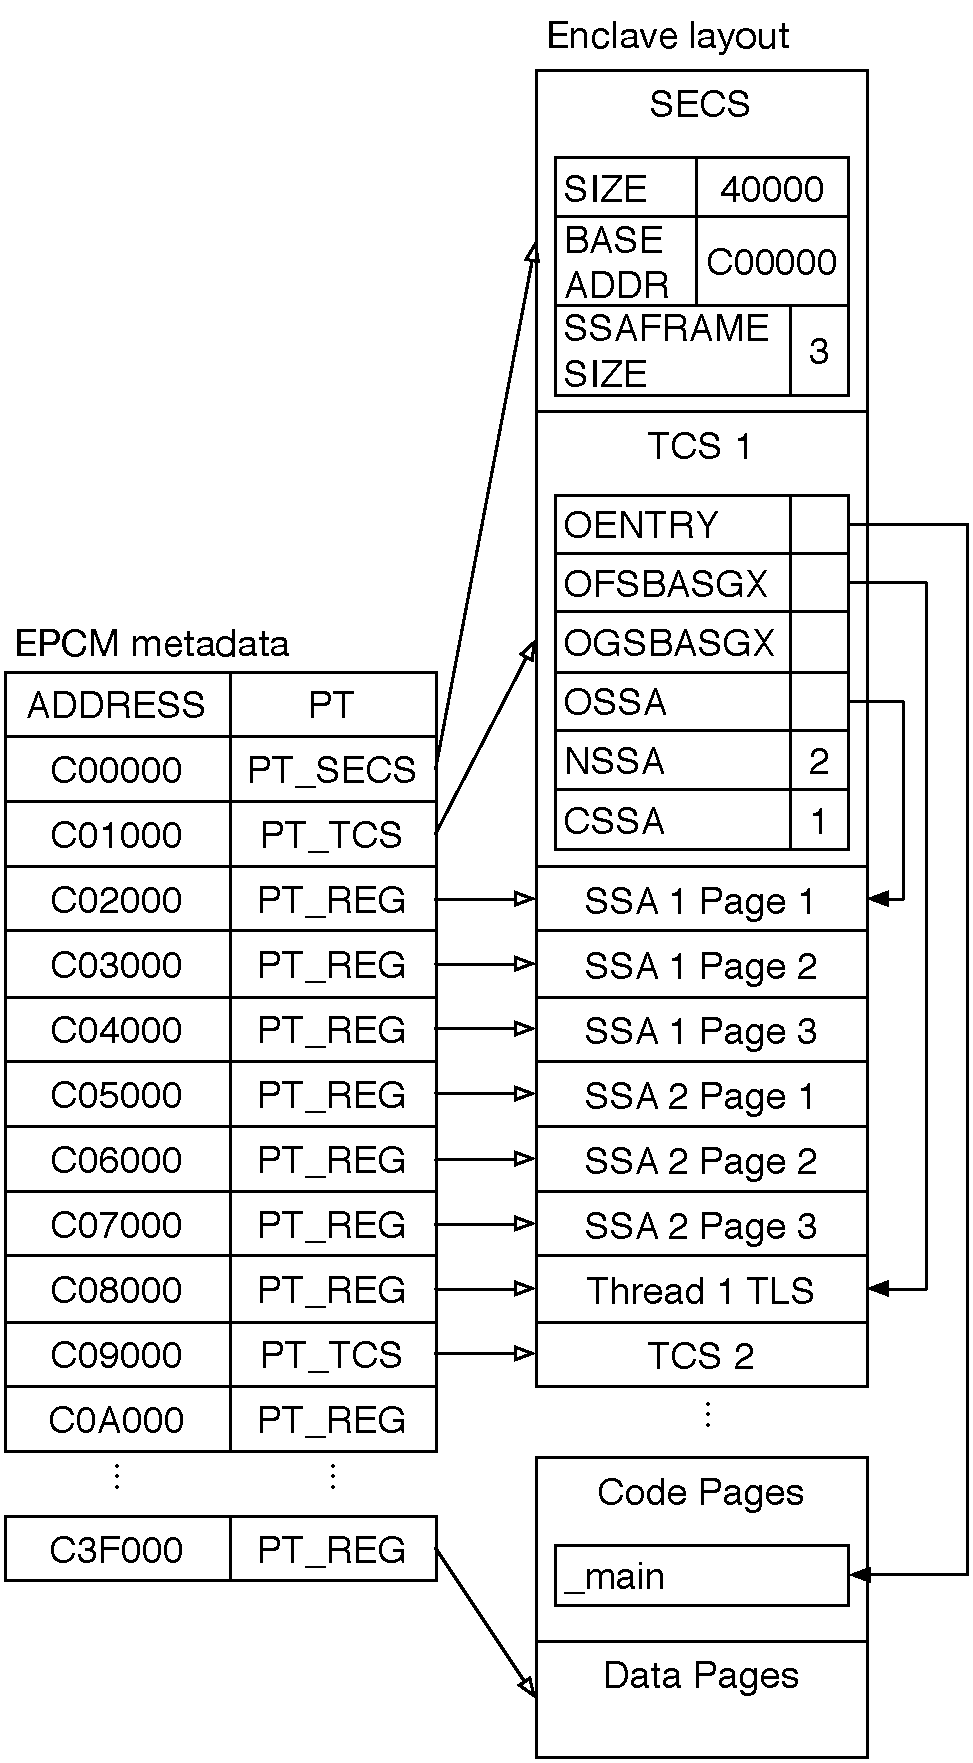
\includegraphics[width=70mm]{figures/enclave_layout.pdf}
  \caption{
    An enclave's memory layout. Each enclave has a SECS, and one TCS per
    supported hardware thread. Each TCS points to a sequence of SSAs, and
    specifies initial values for RIP, FS and GS.
  }
  \label{fig:enclave_layout}
\end{figure}

\subsubsection{The SGX Enclave Control Structure (SECS)}
\label{sec:secs}

% Data Structures and Enclave Operation: SDM S 37.4
% SGX Enclave Control Structure (SECS): SDM S 38.7, S 38.7.1
% Constructing an Enclave: SDM S 39.1
% ECREATE: SDM S 39.1.1, S 41.3
% Implicit vs. Explicit accesses: SDM S 38.5.3
% Implicit accesses: SDM S 38.5.3.2

The first step in creating an enclave is using the \texttt{ECREATE} instruction
to designate a previously unused EPC page as the enclave's \textit{SGX Enclave
Control Structure} (SECS). All instructions that operate on an enclave access
its control structure directly or indirectly.

% Internal CREGs: SDM S 41.1.4
% ECREATE: SDM S 39.1.1, S 41.3
% EWB: SDM S 41.3

The most important field in the SECS is the 64-bit \textit{enclave ID} (EID),
which is assigned by \texttt{ECREATE}. The EID identifies an enclave's pages in
the EPCM, so it must be unique across all the computer's active enclaves.
According to the ECREATE pseudo-code in the SDM, enclave IDs are allocated
using an atomic counter. An enclave's EID is generally hidden, as most SGX
instructions use the address of the enclave's SECS page as the enclave's
handler. However, the system software can learn an enclave's EID by evicting
one of its EPC pages (\S~\ref{sec:sgx_ewb}).

The software-visible SECS layout specifies the range of virtual addresses that
can be mapped to the enclave's EPC pages. Intel documentation calls the range
\textit{enclave linear address range} (ELRANGE). The range is specified using a
base (the BASEADDR field) and a size (the SIZE) field. ELRANGE must meet the
same constraints as a variable memory type range
(\S~\ref{sec:cacheability_config}), namely the size must be a power of 2, and
the base must be aligned to the size.

Currently, the main implication of ELRANGE is that all the SGX data structures
are initialized with enclave virtual addresses specified relatively to
BASEADDR. Furthermore, BASEADDR is not a part of the enclave's measurement
hash (details in \S~\ref{sec:measurement}). It follows that system software can
relocate an enclave in its host application's virtual address space, without
impacting the enclave's measurement hash.

Having ELRANGE follow the memory type range constraints provides a cheap way to
verify if a virtual address belongs to the address, in hardware. This provides
SGX engineers the option to implement per-enclave page tables in future SGX
revisions.

% Interactions with the Processor Extended State and Misc State: SDM S 42.7
% SECS.ATTRIBUTES.XFRM: SDM S 42.7.2.1

The software-visible SECS has an ATTRIBUTE field that specifies the Intel
achitecture features used by the enclave code. For example, the MODE64BIT flag
is set if the enclave targets the 64-bit Intel architecture, and the XFRM
sub-field contains the XCR0 register value expected by the enclave's code. XCR0
controls Intel architecture extensions such as SSE and AVX (see
\S~\ref{sec:registers}).

When a logical processor executes code inside an enclave, it sets XCR0 to the
value specified by the enclave's SECS, so malicious system software cannot
enable features that the enclave code is not prepared to handle. This lets
Intel introduce extensions that change the architectural behavior of existing
instructions, such as Memory Protection Extensions (MPX), without having to
worry about introducing security vulnerabilities in SGX enclaves written before
MPX.

The other fields in the software-visible SECS layout are used by the
software attestation process, which is explained in \S~\ref{sec:attestation}.


\subsubsection{The Thread Control Structure (TCS)}
\label{sec:tcs}

% Thread Control Structure (TCS): SDM S 38.8, S 38.8.{1,2,3,4}

A logical processor uses a \textit{Thread Control Structure} (TCS) while
executing code inside an enclave, so enclave authors must provision at least as
many TCS instances as the number of concurrent software threads that they want
to use.

The fields in the software-visible TCS layout direct the context switches
performed by a logical processor when it transitions between non-enclave and
enclave code.

% State Save Area (SSA): SDM S 38.9

In some cases (e.g., when receiving an interrupt), the processor needs to
preempt the execution of enclave code and start running kernel code. This is
accomplished by saving the enclave's context (register values) to an area
inside the enclave, called a \textit{State Save Area} (SSA).

Each TCS references a contiguous sequence of SSAs -- the OSSA field points to
the first SSA, and the NSSA field indicates the sequence's length. When a
logical processor needs to preempt enclave code, it uses the next available
SSA, indicated by the CSSA field in the TCS. The CPU refuses to execute enclave
code using a TCS where no SSA is available (CSSA $\ge$ NSSA).

An SSA essentially consists of the values of the general-purpose registers
(GPRs), and the result of running XSAVE (\S~\ref{sec:registers}) using the
feature mask specified in the ATTRIBUTES.XFRM field in the enclave's SECS.

% SECS.SSAFRAMESIZE: SDM S 42.7.2.2

Each SSA starts at the beginning of an EPC page, and takes up a fixed number of
EPC pages, specified in the SSAFRAMESIZE field in the enclave's SECS. The SSA
alignment and size restrictions most likely exist to simplify the SGX
implementation.

The TCS is stored in a page whose EPCM entry has the type PT\_TCS, and
therefore cannot be directly accessed by enclave software. However, SSAs are
stored in regular pages, so they are accessible to enclave software, and their
layout is defined in the SGX documentation.

\subsubsection{The Version Array (VA)}
\label{sec:va}

SGX includes support for system software to evict any EPC page to non-EPC RAM,
making it possible to have enclaves whose memory requirements exceed the
computer's EPC size. This is similar to ``swapping'', where the kernel evicts
pages of RAM to a hard disk while they are not accessed.

% Version Array (VA): SDM S 38.18
% EPC and Management of EPC Pages: SDM S 39.5, 39.5.{2,3,4,5,6}

The EWB instruction evicts an EPC page to non-EPC memory. In the process, it
creates an 8-byte nonce (called \textit{page version} in the Intel
documentation), which must be stored in an unused slot of a \textit{Version
Array} (VA). Evicted pages are brought back into the EPC by the ELDU and ELDB
instructions, which use the nonce produced by EWB, and clear the VA slot that
held the nonce.

System software uses the EPA instructions to mark an unused EPC page as a VA.
Pages that store VAs have the PT\_VA EPCM type, so the nonces generated by EWB
cannot be read, even by enclave software.  A VA page has 512 8-byte slots.
Unused slots are marked by the value 0 (zero), and EPA zeroes out the EPC page
used to store the VA.

Non-EPC memory can be accessed by system software, which is untrusted in the
SGX threat model, so EWB (illustrated in Figure~\ref{fig:sgx_ewb}) encrypts and
MACs the contents of the EPC page before storing it in untrusted memory. The
nonces stored in VA pages prevent replay attacks where malicious system
software would attempt to bring back an old version of an evicted EPC page.


\subsection {The Implementation of EPC Protection}

The memory controller is
integrated on the CPU die (see Figure~\ref{fig:cpu_die}), so it can be trusted
to prevent devices attached to the system bus from performing DMA transfers
to/from the PRM.

System software manages physical memory by directly modifying the contents of
page tables and EPTs (\S~\ref{sec:paging}), and is responsible for performing
TLB shootdowns (\S~\ref{sec:tlbs}) to ensure that the state not covered by
cache coherence \S~\ref{sec:cache_coherence} is synchronized across logical
processors. If the system software does not perform TLB shootdowns correctly,
application software can experience inconsistent views of memory.

In the context of SGX, an incorrect TLB shootdown can can result in having an
EPC page simultaneously accessible by two different enclaves, which would
compromise the SGX security guarantees. Therefore, the SGX instructions used
for EPC management ensure that the system software performs TLB shootdowns for
the entries that represent EPC pages.


% PRMRR documented in HASP papers and both SGX manuals, completely removed from
% SDM. It still exists in Coreboot. Couldn't find other Skywell code.
The SGX manual states that the EPC (the memory used to store enclave data) can
only be set up as UC or WB. While no further explanation is provided, we assume
that the UC option was provided in order to attempt to mitigate against some
cache-timing attacks.




\section{Security Analysis}
\label{sec:security}

The rest of this section describes the security properties of
enclaves, discussing the trade-offs made while trying to balance security with
backwards compatibility.

% Interactions with Paging: SDM S 42.4
% The Intel SGX access control itself is implemented as an extension to the
% three paging modes of Intel Architecture.

% Page-Based Access Control: SDM S 38.5

% ECREATE forces R, W, X to 0 in the page's EPCM. EADD also forces R/W/X to 0
% if the page type in SECINFO is PT_TCS (the only special type it can create).
%
%
% EPA doesn't read any SECINFO, and uses 0 for R, W, X.

% ERESUME can be replaced by normal EENTER, XRESTOR and accounting. Describe
% and argue against ERESUME.


% The use of the page version (nonce) as counter in AES-GCM makes it impossible
% for malicious system software to determine whether an EPC page's contents has
% changed between two evictions.
% However, the dirty bit in the EPC page's PTE will leak that information.

% According to the ECREATE pseudo-code in the Intel manual, EIDs are assigned
% using a counter that is atomically incremented on every ECREATE. This makes
% the field predictible to system software.


% The SGX instruction that evicts an EPC page, EWB, ensures that the VA slot it
% is supposed to write is unused.
% The VA unused slot check in EWB is unnecessary. Bad system software can only
% overwrite a version and impair its ability to restore a page.

Enclaves were designed to contain and protect the privacy-sensitive parts of an
application. All the code that handles private data must receive integrity
protection. Otherwise, a hostile environment could modify the code to leak
information about private data. Therefore, the SGX programming model prescribes
that code which accesses private data must be entirely contained inside an
enclave. Jumping into and out of enclave code must be performed explicitly
using the dedicated instructions \texttt{EENTER} and \texttt{EEXIT}.



\begin{figure}[hbt]
  \centering
  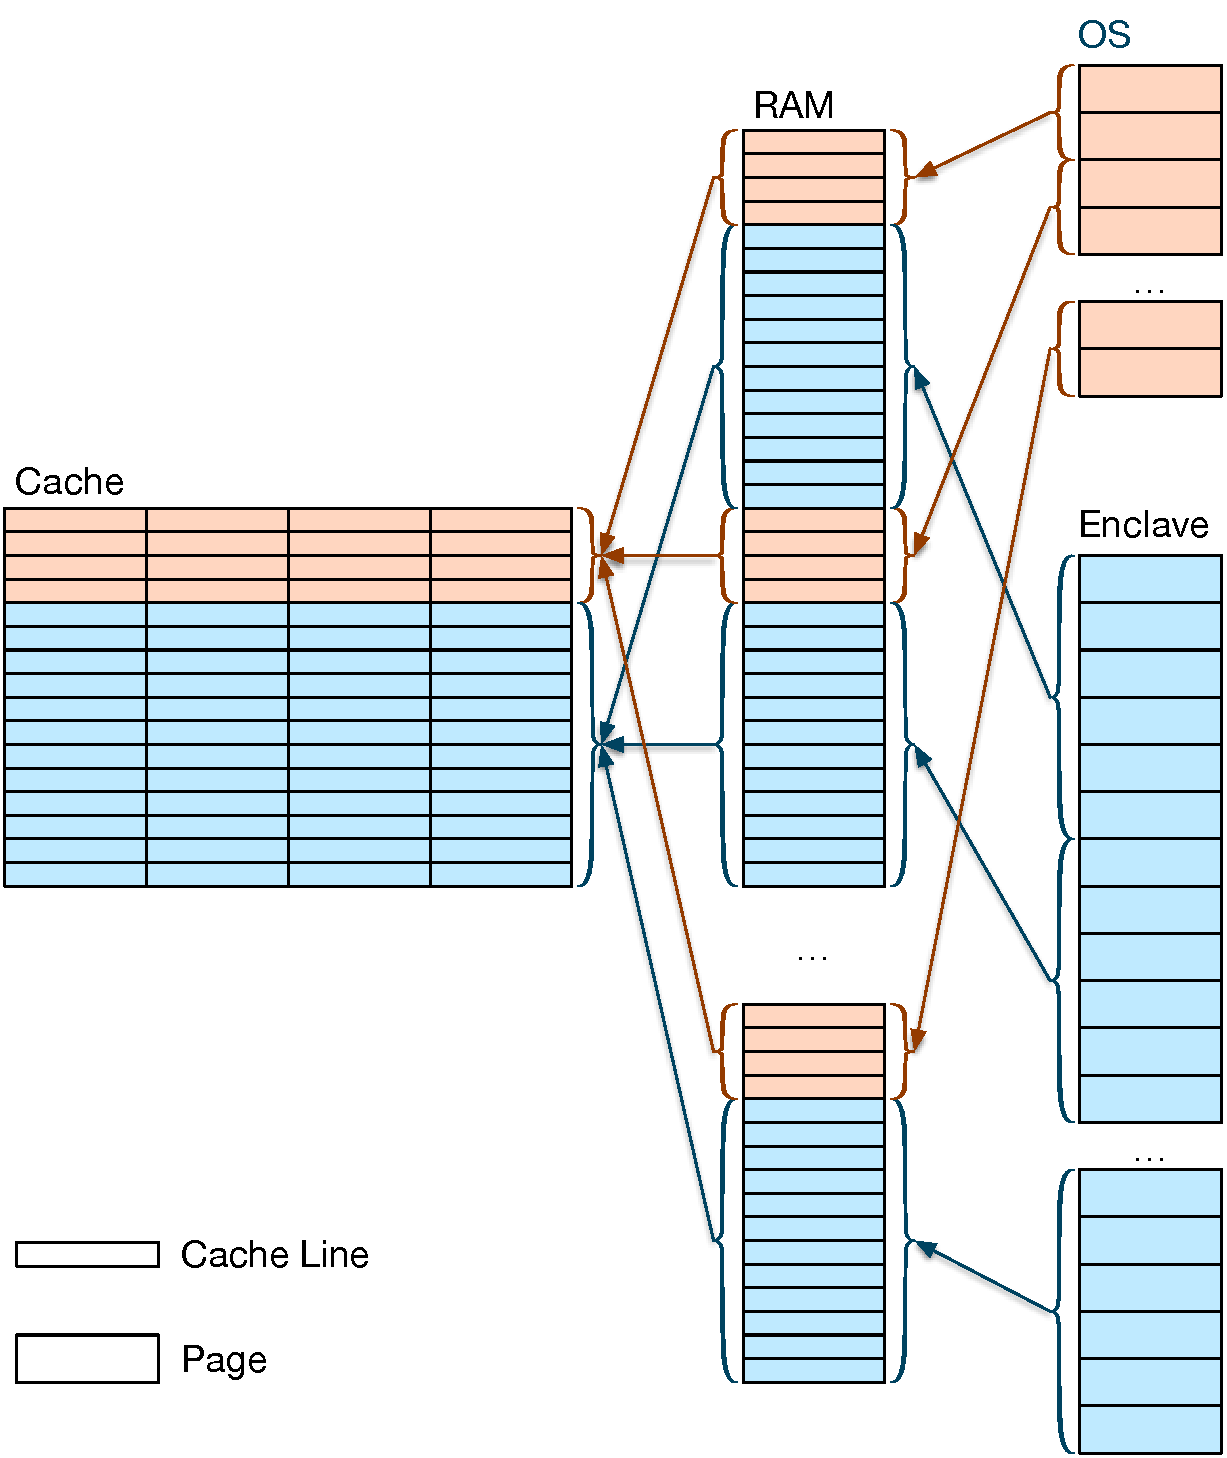
\includegraphics[width=85mm]{figures/cache_partitions.pdf}
  \caption{
    Cache partitioning between two applications. Each application has some
    cache sets allocated to it, and only uses RAM regions that map to its cache
    sets. When partitioning the L1 cache, applications have to follow this
    constraint themselves. When the L2 cache is partitioned, the OS can map the
    pages in an application's virtual address space to the RAM regions that the
    application can use, so applications are oblivious to the cache
    partitioning.
  }
  \label{fig:cache_partitions}
\end{figure}


\setlength{\bibsep}{1pt}
\small
\bibliographystyle{plain}
%\bibliographystyle{abbrv}
%\bibliographystyle{ieeetr}
\bibliography{references}

\end{document}
